\documentclass[a4paper,12pt,twoside]{article}

\renewcommand{\title}{Esercitazioni di Aerodinamica sperimentale}
\renewcommand{\author}{Alessio Improta}
% \renewcommand{\familydefault}{\sfdefault}

\usepackage[english, italian]{babel}
\usepackage[T1]{fontenc}
\usepackage[utf8]{inputenc}
\usepackage[top=3cm,bottom=4cm,inner=3cm,outer=2.5cm]{geometry}
\usepackage{mathtools}
\usepackage{amsfonts}
\usepackage{graphicx}
\usepackage{matlab-prettifier}
\usepackage[colorlinks=true, allcolors=black, pdfusetitle, pdftex,
            pdfsubject={\title},
            pdftitle={\title},
            pdfauthor={\author},
            pdfkeywords={Politecnico di Torino, Ingegneria aerospaziale, \title}]{hyperref}
\usepackage{lastpage} % per usare \pageref{LastPage}
\usepackage{fancyhdr} % per modificare intestazioni e piè di pagina
\usepackage[nottoc, notlof, notlot]{tocbibind} % per modifiche all'indice
\usepackage[superscript]{cite} % riferimenti bibliografici in apice
\usepackage{listings} % per usare \begin{lstlisting}
\usepackage{xcolor}
\usepackage{float}
\usepackage{titlesec} % per modificare la dimensione dei titoli dei capitoli e sottotitoli
\usepackage{bm} % simboli in grassetto
\usepackage{lipsum} % per usare \lipsum
\usepackage{scalerel}
\usepackage{tikz} % per tracciare diagrammi
\usetikzlibrary{arrows.meta} % per utilizzare freccie
\hbadness=100000 % Per ignorare avvertimenti

% Dimensione titoli dei capitoli e sottocapitoli
\titleformat*{\section}{\LARGE\bfseries}
\titleformat*{\subsection}{\Large\bfseries}
\titleformat*{\subsubsection}{\large\bfseries}
\titleformat*{\paragraph}{\bfseries}
\titleformat*{\subparagraph}{\bfseries}

% Syntax Highlighter per Python
\definecolor{codegreen}{rgb}{0,0.6,0}
\definecolor{codegray}{rgb}{0.5,0.5,0.5}
\definecolor{codepurple}{rgb}{0.58,0,0.82}
\lstset{
    language=Python,
    commentstyle=\color{codegreen},
    keywordstyle=\color{blue},
    numberstyle=\ttfamily\footnotesize\color{codegray},
    stringstyle=\color{codepurple},
    basicstyle=\ttfamily\footnotesize,
    breakatwhitespace=false,         
    breaklines=true,                 
    captionpos=b,                    
    keepspaces=true,                 
    numbers=left,                    
    numbersep=5pt,                  
    showspaces=false,                
    showstringspaces=false,
    showtabs=false,                  
    tabsize=2
}

% Alias dei comandi
\newcommand{\dt}[1]{\dfrac{\partial #1}{\partial t}}
\newcommand{\dx}[1]{\dfrac{\partial #1}{\partial x}}

\begin{document}

% FRONTESPIZIO
\pagenumbering{arabic}
\pagestyle{empty}
\newgeometry{right=2.5cm,left=2.5cm,top=3cm,bottom=4cm}

\vspace{.4cm}

\begin{center}
    
\includegraphics[width=.46\textwidth]{images/polito.png}
\end{center}

\vspace{.2cm}

\begin{center}
    \Large{\textbf{POLITECNICO DI TORINO}}\\
    \vspace{0.2cm}
    \large{\textbf{CORSO DI LAUREA MAGISTRALE IN INGEGNERIA AEROSPAZIALE}}
\end{center}

\vspace{2.5cm}

\begin{center}
    \LARGE{\textbf{ESERCITAZIONI DI\\AERODINAMICA SPERIMENTALE}}
\end{center}

\vspace{2cm}

\begin{flushleft}
    \linespread{1}
    \large{\textbf{Docente \hfill Studente}\\
    \textbf{Prof. Gaetano Iuso \hfill Alessio Improta\\
    \hfill Matr. 315411}
    }
\end{flushleft}

\vfill

\begin{center}
    \large{\textbf{ANNO ACCADEMICO 2023-2024}}
\end{center} 

\clearpage
\restoregeometry

% PAGINA BIANCA DOPO FRONTESPIZIO
\newpage
\thispagestyle{empty}
\mbox{}

% INDICE
\newpage
\pagestyle{plain}
\pagenumbering{Roman}
\tableofcontents

% PAGINA BIANCA DOPO INDICE
\newpage
\thispagestyle{empty}
\mbox{}

% CONTENUTO
\newpage
\pagenumbering{arabic}
\pagestyle{fancy}
\renewcommand{\headrulewidth}{0pt}
\renewcommand{\footrulewidth}{0.4pt}
\fancyhf{}
\fancyfoot[L]{Aerodinamica sperimentale --- \author}
\fancyfoot[R]{Pagina \thepage\ di \pageref{LastPage}}
\setlength{\headheight}{13.6pt}

\thispagestyle{fancy}
\section{Taratura di un trasduttore di pressione}
Il trasduttore di pressione è un componente della catena di misura preposto a quantificare il valore della pressione da misurare sfruttando un principio fisico.\\\\
La pressione misurata può essere riferita al vuoto (nel caso di trasduttori assoluti) oppure rispetto ad una pressione di riferimento (nel caso di trasduttori differenziali).\\\\
L'obiettivo del presente esperimento è la taratura di un trasduttore differenziale capacitivo bidirezionale ad alta precisione, il SETRA mod. 239 C.
\begin{figure}[h]
    \centering
    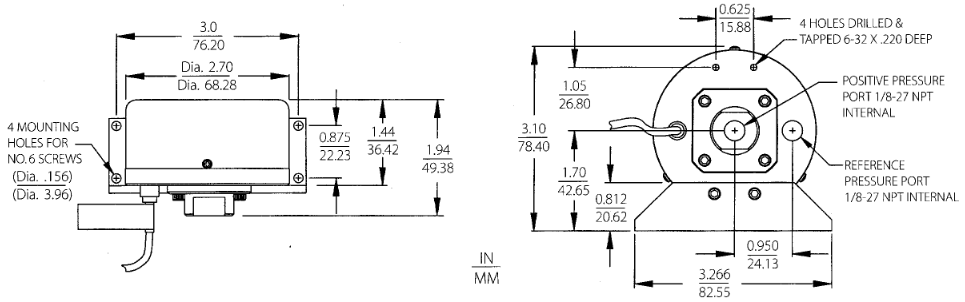
\includegraphics[width=\linewidth]{images//1/setra.png}
    \caption{Trasduttore di pressione SETRA mod. 239 C}
\end{figure}

\subsection{Descrizione dell'esperimento}
I trasduttori differenziali misurano una differenza di pressione $p-p_{rif}$ e presentano pertanto due ingressi, uno per la pressione da misurare ed uno per la pressione di riferimento. La pressione di riferimento viene definita dall'operatore a seconda della misura da effettuare. Nel caso in esame, questa è la pressione statica della corrente nel cuore potenziale di un getto.\\\\
Nei trasduttori capacitivi viene sfruttata la variazione di capacità di un condensatore sotto l'effetto della forza di pressione. Una faccia del condensatore è fissa mentre l'altra è flessibile e per effetto dell'azione di pressione agente su di essa si deforma variando la distanza tra le due facce e quindi la capacità.\\\\
Alla variazione della capacità $C(t)$ è legata la variazione del segnale elettrico in uscita, che tipicamente è una tensione $E(t)$. La capacità di un condensatore è definita dalla seguente relazione:
\begin{equation*}
    C = \frac{K_d A}{X_0}
\end{equation*}
in cui $K_d$ è la costante dielettrica della capacità, $A$ è la superficie della parete e $X_0$ è la distanza tra le facce del condensatore. Per effetto della deformazione, varia la distanza $X_0$ tra la membrana flessibile e la parte fissa. Ad una variazione della capacità $\Delta C$ corrisponde pertanto una variazione di potenziale ai capi del condensatore:
\begin{equation*}
    \Delta V = \frac{\Delta C}{C}E_a
\end{equation*}
dove $\Delta C/C$ è la variazione della capacità dovuta alla pressione mentre $E_a$ è la tensione di alimentazione del condensatore. Risulta pertanto $\Delta V = f(\Delta p)$.\\\\
Il legame tra la differenza di pressione $\Delta p$ e la differenza di tensione $\Delta V$ prende il nome di curva di taratura del trasduttore. Il segnale elettrico e la pressione applicata sono correlate attraverso una costante di taratura $K_t$ che va determinata sperimentalmente.\\\\
Eseguire la taratura del trasduttore significa quindi determinare il valore della costante di taratura $K_t$.

\subsection{Catena di misura}
Per effettuare la taratura del trasduttore, e quindi trovare una relazione che associa ad ogni valore di tensione in uscita un valore di differenza di pressione applicata, è necessario conoscere l'entità di tale pressione. Si utilizza quindi un flusso noto: il cuore potenziale di un getto.
\begin{figure}[H]
    \centering
    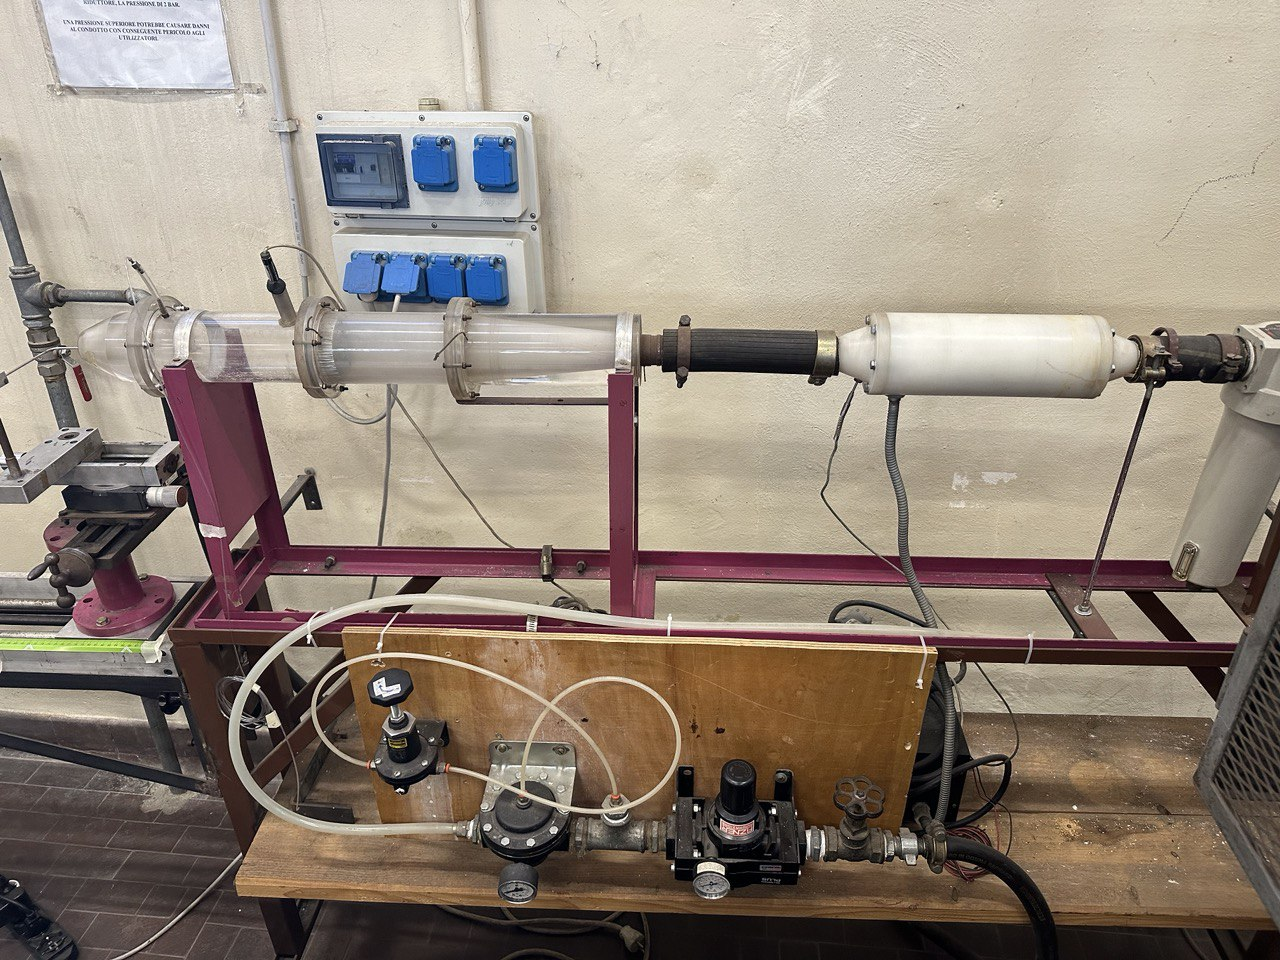
\includegraphics[width=.8\textwidth]{images/1/getto.jpg}
    \caption{Sistema di regolazione della portata del getto}
\end{figure}

\noindent Per rilevare la pressione totale e la pressione statica nel cuore potenziale del getto è utilizzato un tubo di Pitot.
\begin{figure}[H]
    \centering
    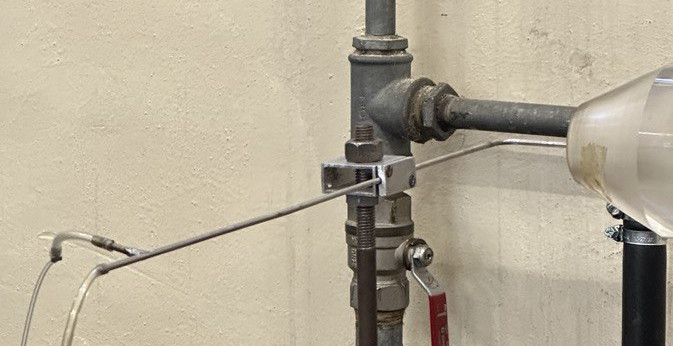
\includegraphics[width=.45\textwidth]{images/1/pitot.jpg}
    \caption{Tubo di pitot nel cuore potenziale del getto}
\end{figure}

\noindent Per ricavare il corretto valore di differenza di pressione dal tubo di Pitot si utilizza il manometro di Betz, uno strumento di grande precisione costituito da un serbatoio di acqua distillata entro cui è presente una scala graduata galleggiante. La differenza di pressione tra due camere entro cui è contenuto il liquido produce uno spostamento verticale del galleggiante.
\begin{figure}[h]
    \centering
    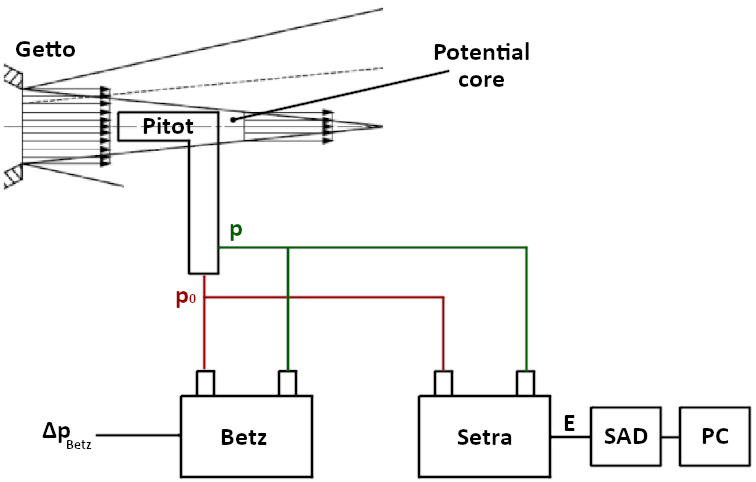
\includegraphics[width=.7\textwidth]{images/1/catena.png}
    \caption{Catena di misura}
\end{figure}

\noindent La catena di misura è quindi composta da:
\begin{itemize}
    \item Getto;
    \item Tubo di Pitot, posizionato nel cuore potenziale del getto;
    \item Trasduttore di pressione SETRA mod. 239 C; 
    \item Manometro di Betz;
    \item Sistema di acquisizione dati (SAD) e PC con LabView.
\end{itemize}

\noindent I canali pneumatici di pressione statica e pressione totale rilevate dal tubo di Pitot sono connessi sia al manometro di Betz che al trasduttore di pressione SETRA mod 239 C. Pertanto, tramite il sistema di acquisizione dati, è possibile registrare il valore di tensione in uscita ed associarlo alla relativa differenza di pressione indicata dal manometro di Betz.\\\\

\subsection{Procedura sperimentale}
Come prima operazione è necessario misurare la tensione di offset $E_0$, cioè la tensione in uscita al trasduttore quando non è applicata alcuna differenza di pressione. Per fare ciò, si acquisiscono i dati in uscita al trasduttore con il getto spento. Si ottiene la seguente tensione di offset:
\begin{equation*}
    E_0 = -8.57\cdot 10^{-4}\ V
\end{equation*}
Una volta misurata tale tensione, si può scomporre il segnale in uscita come:
\begin{equation*}
    E(\Delta p) = E_0 + \Delta E(\Delta p)
\end{equation*}
Si procede variando la portata e quindi la pressione dinamica nel cuore potenziale del getto ed acquisendo per ogni valore di differenza di pressione indicato sul manometro di Betz il valore di tensione in uscita corrispondente.\\\\
Il manometro di Betz è caratterizzato da una bassa risposta in frequenza, pertanto per ogni variazione di portata del getto è necessario attendere almeno 30 secondi per fare in modo che il manometro di Betz riporti il valore di differenza di pressione corretto sulla scala graduata.\\\\
I dati sono acquisiti con una frequenza $f_s=2$ kHz per un periodo di $T=1$ s.\\\\
I dati grezzi acquisiti durante la procedura sono riportati in appendice \ref{a1}.\\\\

\subsection{Analisi dati e costante di taratura}
L'analisi dati è condotta con l'ausilio di un codice Python, riportato in appendice \ref{b1}.\\\\
La relazione che lega la differenza di pressione applicata, misurata con il manometro di Betz, e il segnale di tensione in uscita dal trasduttore di pressione è la seguente:
\begin{equation*}
    \Delta p_{Betz} = K_t \Delta E = K_t (E - E_0)
\end{equation*}
Da cui si ricava:
\begin{equation*}
    K_t = \frac{\Delta p_{Betz}}{\Delta E}
\end{equation*}
\newpage
\noindent I dati sperimentali acquisiti, con le relative barre di errore, sono riportati nel seguente diagramma:
\begin{figure}[h]
    \centering
    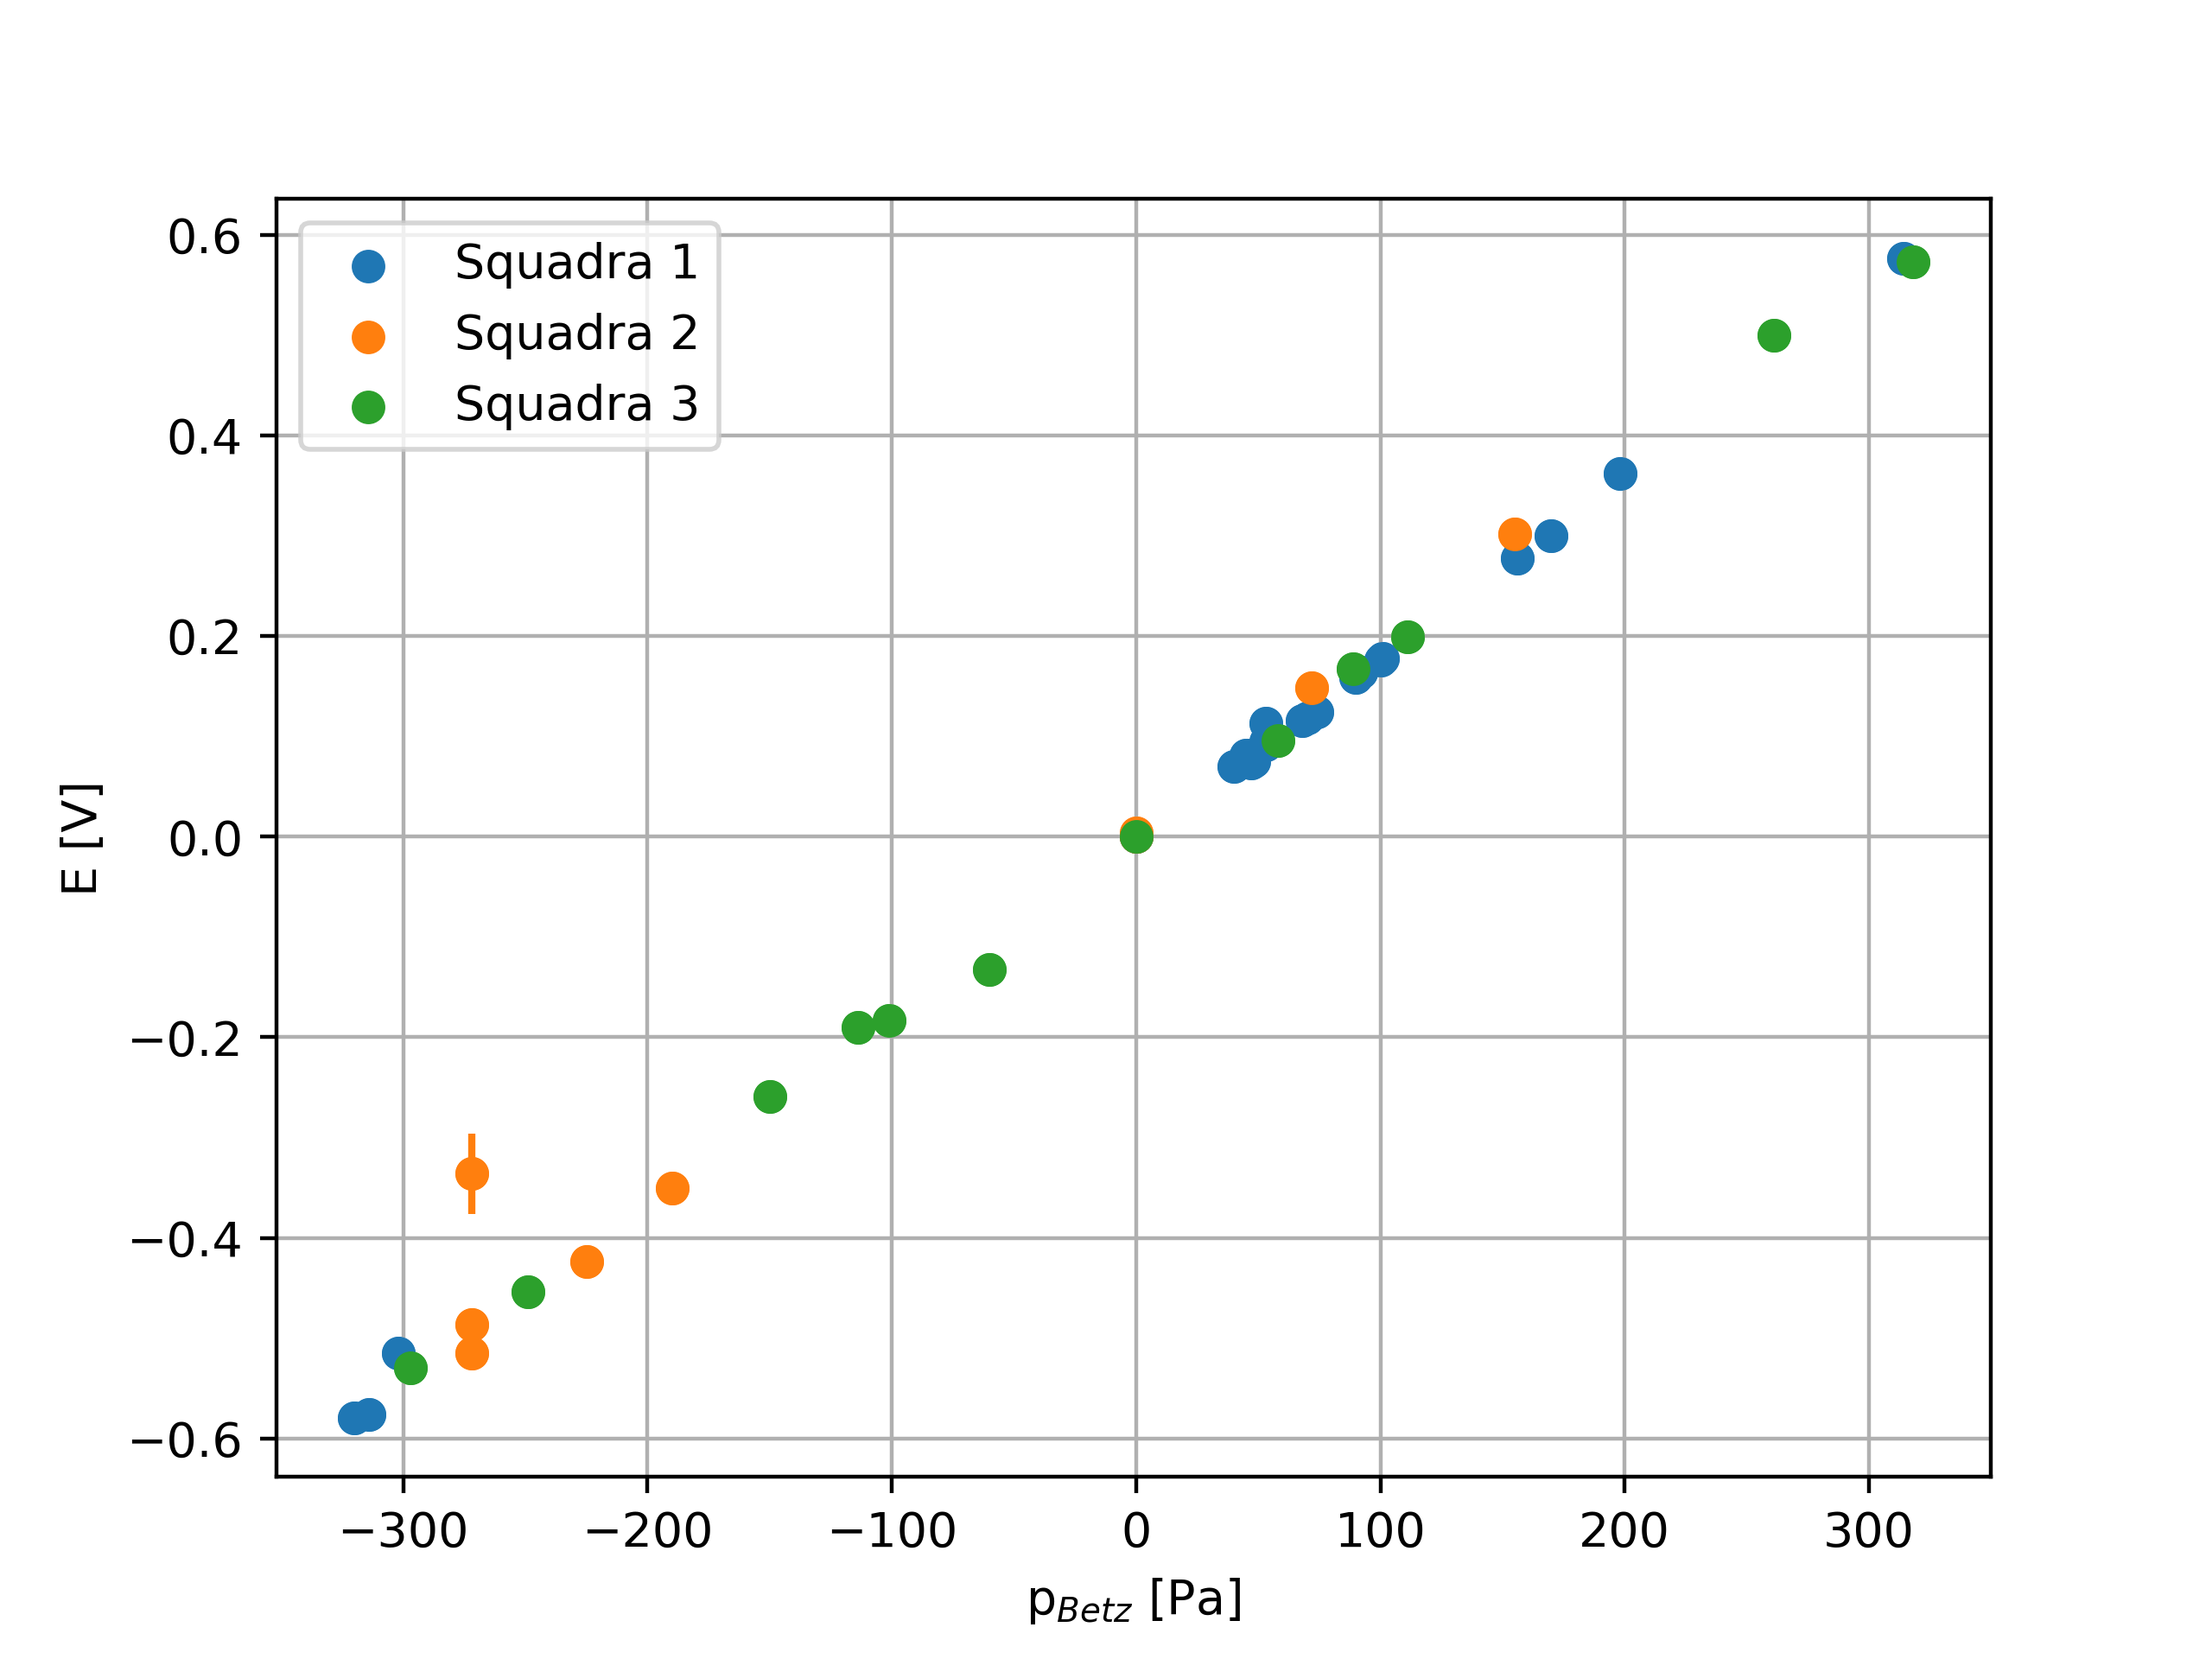
\includegraphics[width=\textwidth]{images/1/kt.png}
    \caption{Dati sperimentali}
\end{figure}

\noindent Attraverso una semplice interpolazione lineare dei dati, è possibile ricavare il valore sperimentale della costante di taratura per le tre squadre:

\begin{equation*}
    \text{Squadra 1: } K_t = 556.69\ \text{Pa/V}
\end{equation*}
\begin{equation*}
    \text{Squadra 2: } K_t = 549.38\ \text{Pa/V}
\end{equation*}
\begin{equation*}
    \text{Squadra 3: } K_t = 549.47\ \text{Pa/V}
\end{equation*}
Per semplicità, nelle seguenti esercitazioni la costante di taratura è imposta pari a
\begin{equation*}
    K_t = 550\ \text{Pa/V}
\end{equation*}

\newpage
\subsection{Tempo caratteristico}
Poiché il manometro di Betz è caratterizzato da una lenta risposta in frequenza, è opportuno indagare il fenomeno transitorio della linea pneumatica ed il relativo tempo caratteristico $\tau$.\\\\
Per fare ciò, sono acquisite le tensioni di uscita dal trasduttore con una frequenza di campionamento $f_{samp}=2000$ Hz per un periodo $T$ di 2 minuti.\\\\
Per determinare il tempo caratteristico si interpolano i dati sperimentali con una curva esponenziale, del tipo:
\begin{equation*}
    E(t) = Ae^{bt} = Ae^{-\frac t\tau}
\end{equation*}
Maneggiando tale relazione, si ottiene:
\begin{equation*}
    \log E(t) = \log A + bt = c_1 t + c_2 \quad \Rightarrow \quad b = -\frac1\tau = c_1 \ ; \ A = e^{c_2}
\end{equation*}
Si ricava dunque il tempo caratteristico della linea pneumatica:
\begin{equation*}
    \tau = 295.06 \text{s}
\end{equation*}
Il valore ottenuto risulta coerente con la risposta in frequenza del manometro di Betz.
\begin{figure}[h!]
    \centering
    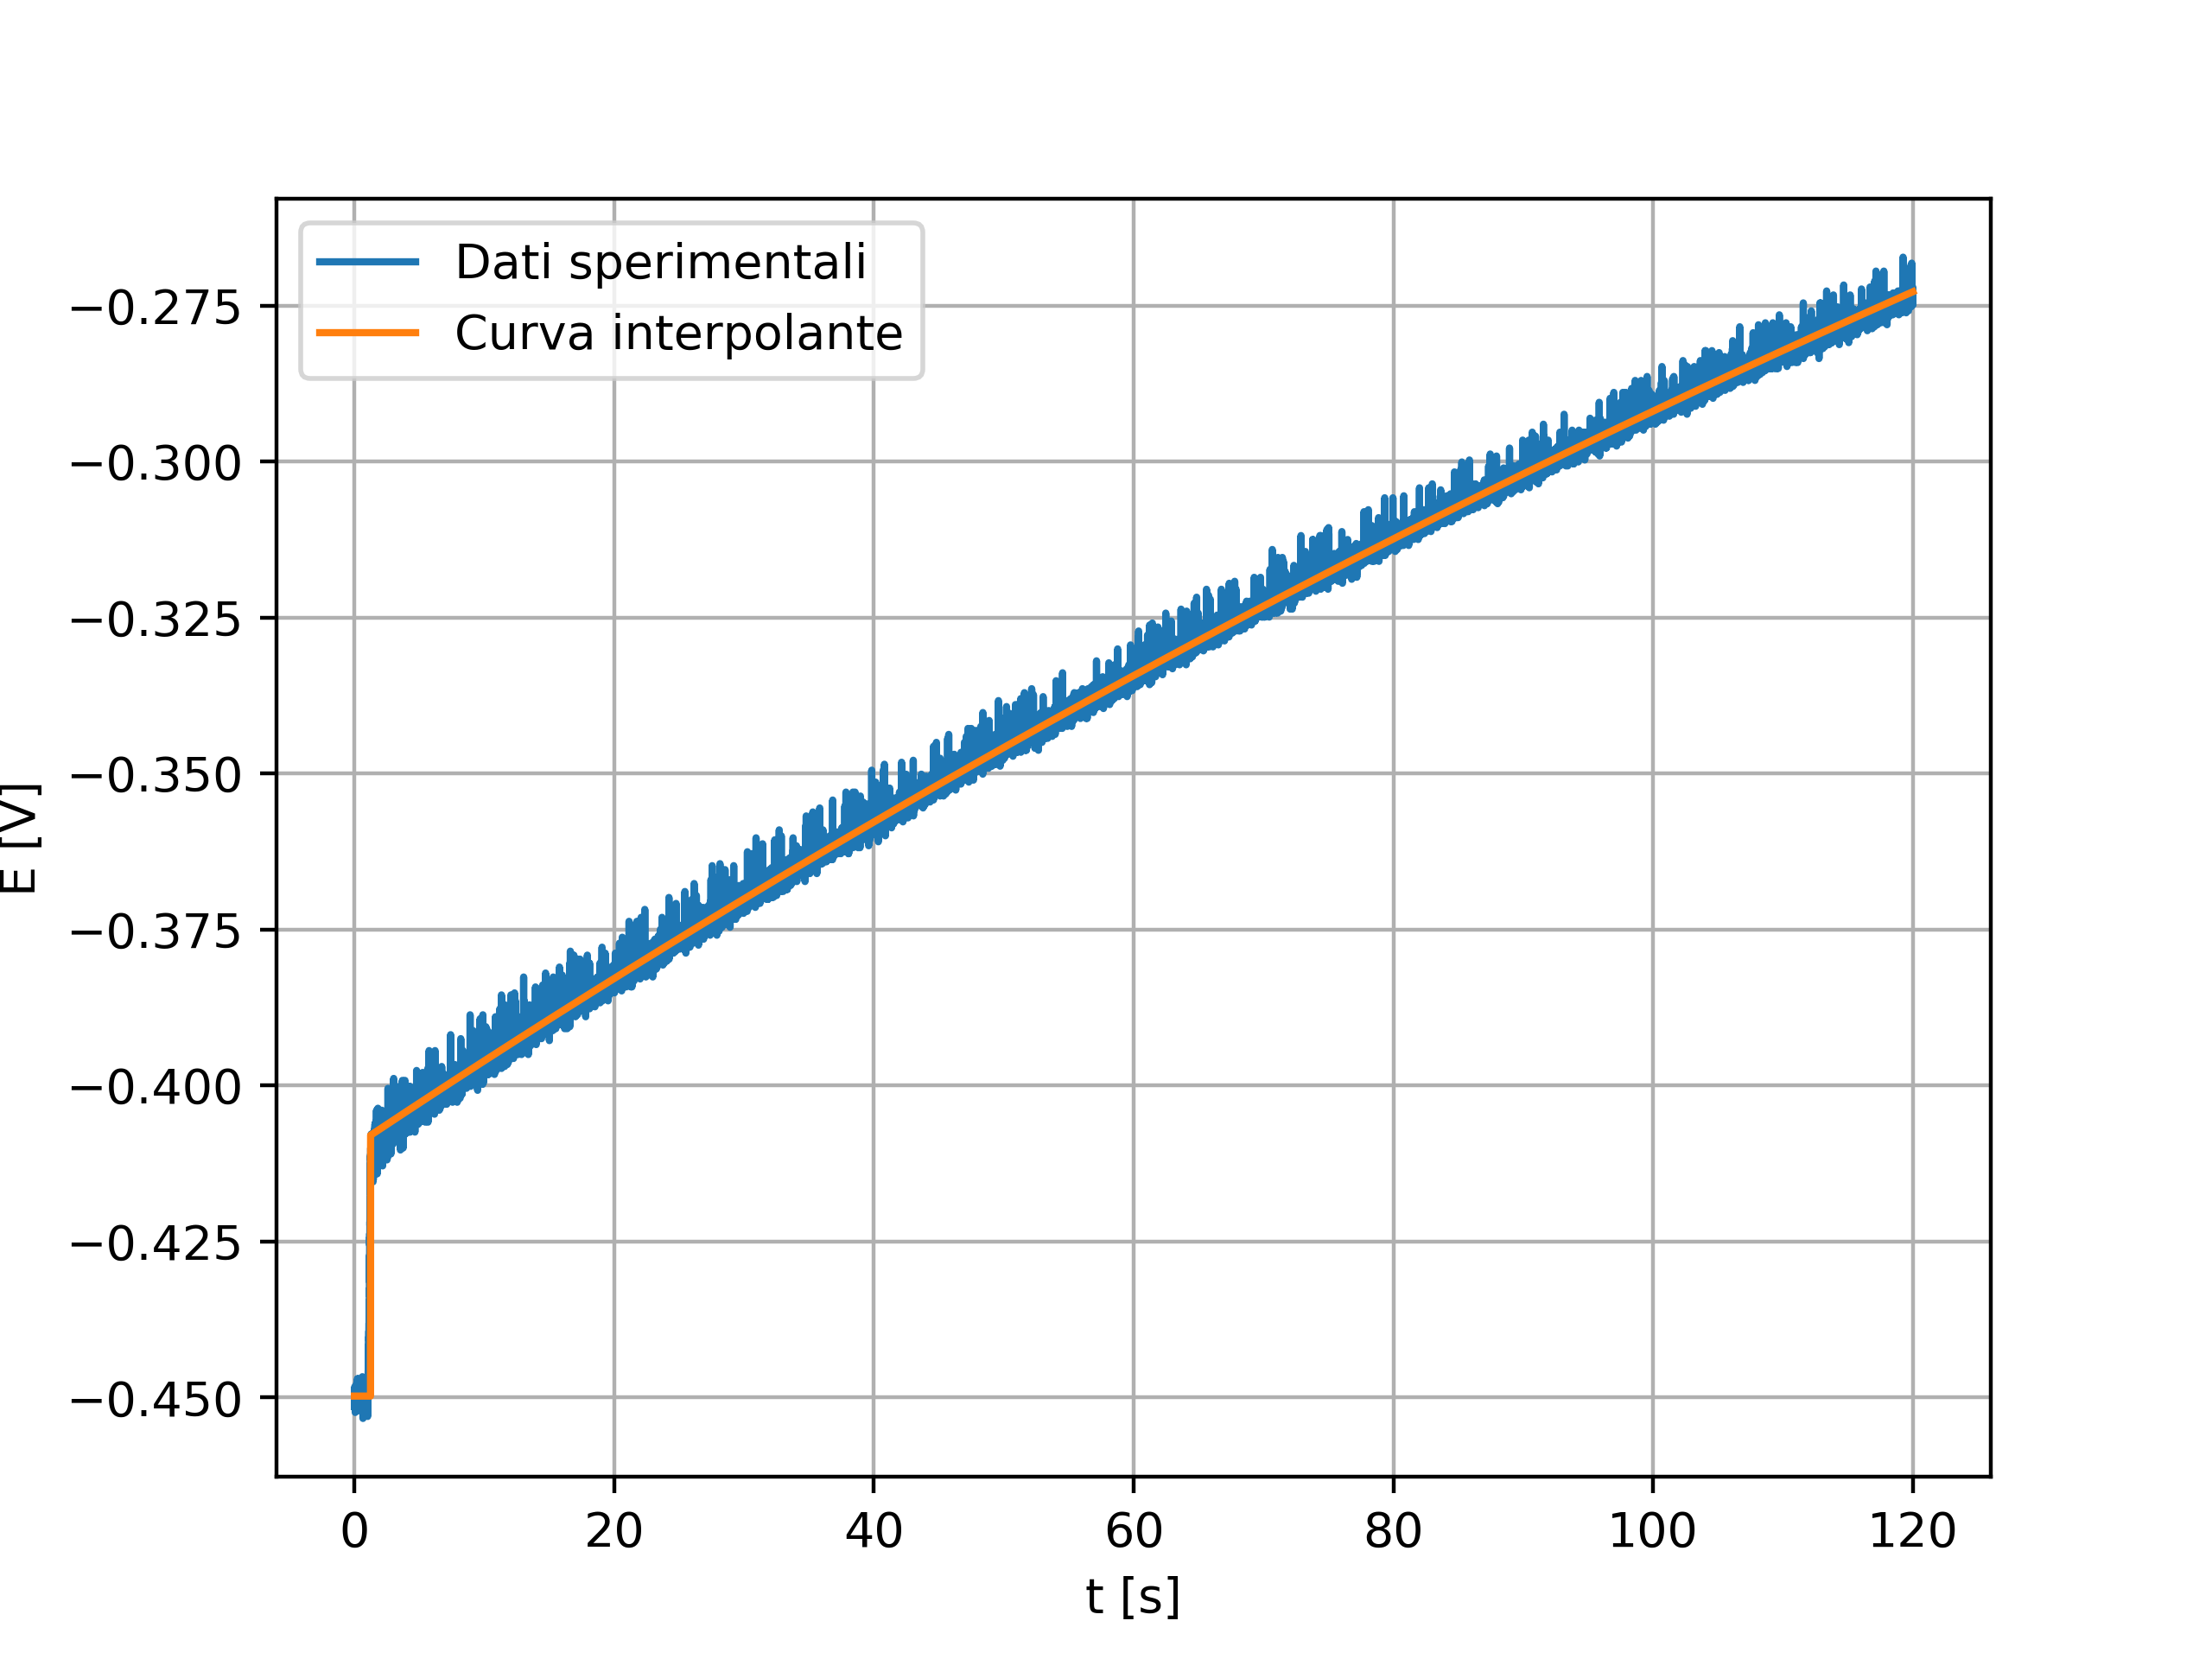
\includegraphics[width=.8\textwidth]{images/1/transitorio.png}
    \caption{Transitorio}\label{fig:t1}
\end{figure}
\section{Risposta direzionale di un tubo di Pitot}
Il tubo di Pitot è una sonda cilindrica con sezione trasversale circolare che viene utilizzata allineata con la corrente. Tale sonda è munita di una presa di pressione totale frontale e di una o più prese di pressione statica (solitamente quattro prese a novanta gradi tra loro) poste sulla superficie cilindrica ad opportuna distanza dall'estremità anteriore.\\\\
La sonda presenta al suo interno due tubi coassiali. In quello più interno si risente la pressione totale mentre sul tubo esterno sono posizionate le prese di pressione statica. All'estremità opposta alla zona di misura della sonda sono presenti due uscite corrispondenti al segnale di pressione statica e a quello di pressione totale, da collegare con un trasduttore di pressione.
\begin{figure}[h]
    \centering
    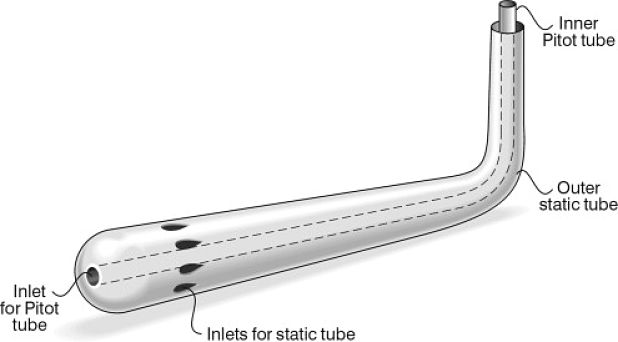
\includegraphics[width=0.55\linewidth]{images/2/pitotsketch.png}
    \caption{Rappresentazione di un tubo di Pitot}
\end{figure}

\subsection{Descrizione dell'esperimento}
La presente esercitazione si pone come obiettivo la caratterizzazione di una sonda di Pitot. In particolare si vuole:
\begin{itemize}
    \item Valutare l'effetto del disallineamento $\alpha$ della sonda sulla pressione totale, sulla pressione statica e sulla pressione dinamica;
    \item Determinare la velocità della corrente;
    \item Valutare l'effetto del numero di Reynolds.
\end{itemize}
\noindent La sonda di Pitot in esame possiede le seguenti caratteristiche geometriche:
\begin{itemize}
    \item Diametro esterno: $D = 3$ mm;
    \item Diametro interno: $d = 1$ mm;
    \item Distanza delle prese statiche dal bordo di attacco: $L_1 = 12.5$ mm;
    \item Distanza delle prese statiche dal gambo: $L_2 = 37$ mm.
\end{itemize}
\newpage
\noindent La valutazione della velocità della corrente si ricava considerando la relazione di Bernoulli:
\begin{equation*}
    p_0 = p + \frac12 \rho V^2 \quad \rightarrow \quad q = p_0 - p = \frac12 \rho V^2
\end{equation*}
Dalla velocità è possibile ricavare il numero di Reynolds della corrente:
\begin{equation*}
    Re = \frac{\rho V D}{\mu}
\end{equation*}
L'errore commesso nella misura delle pressioni in presenza di disallineamento viene valutato definendo prima una grandezza $\varepsilon$ che caratterizza l'entità dell'errore. Si possono pertanto introdurre tre funzioni ognuna riferita alle tre pressioni:
\begin{equation*}
    \varepsilon_{p_0}(\alpha) = \frac{p_0(\alpha) - p_{0,\alpha=0}}{q_{\alpha=0}} \qquad \varepsilon_{p}(\alpha) = \frac{p(\alpha) - p_{\alpha=0}}{q_{\alpha=0}} \qquad \varepsilon_{q}(\alpha) = \frac{q(\alpha) - q_{\alpha=0}}{q_{\alpha=0}}
\end{equation*}

\subsection{Catena di misura}
Analogamente alla precedente esercitazione, il flusso di riferimento per la caratterizzazione della sonda di Pitot è il cuore potenziale di un getto.\\\\
Il tubo di Pitot è connesso al trasduttore di pressione SETRA mod 239 C già precedentemente tarato ($K_t=550$ Pa/V). Per il calcolo della pressione dinamica ai due ingressi del trasduttore sono connessi i canali pneumatici relativi alla pressione totale ed alla pressione statica del tubo di Pitot. Per il calcolo della pressione totale, invece, il canale pneumatico relativo alla pressione statica del tubo di Pitot viene scollegato, così che il trasduttore riceva in ingresso la pressione ambiente. Per il calcolo della sola pressione statica, analogamente, viene scollegato il canale pneumatico relativo alla pressione totale del tubo di Pitot. In questo modo è possibile valutare la pressione totale, la pressione statica e la pressione dinamica nel cuore potenziale del getto.\\\\
Per operare il disallineamento controllato del tubo di Pitot, questo è montato su un goniometro, in modo tale che anche modificando l'angolo $\alpha$ di disallineamento la testa della sonda rimanga nella stessa posizione, il più possibile vicina all'asse del getto.\\\\
La catena di misura è dunque costituita da:
\begin{itemize}
    \item Getto;
    \item Tubo di Pitot, posizionato nel cuore potenziale del getto;
    \item Goniometro opportunamente posizionato;
    \item Trasduttore di pressione SETRA 239 C;
    \item Sistema di acquisizione dati (SAD) e PC con LabView.
\end{itemize}

\newpage
\begin{figure}[ht]
    \centering
    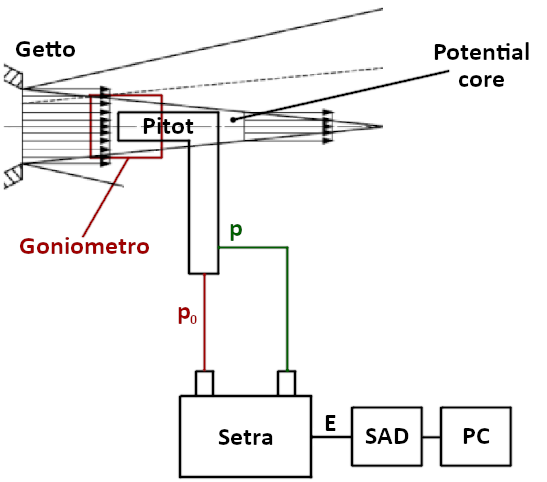
\includegraphics[width=.65\textwidth]{images/2/catena.png}
    \caption{Catena di misura}
\end{figure}
\begin{figure}[h!]
    \centering
    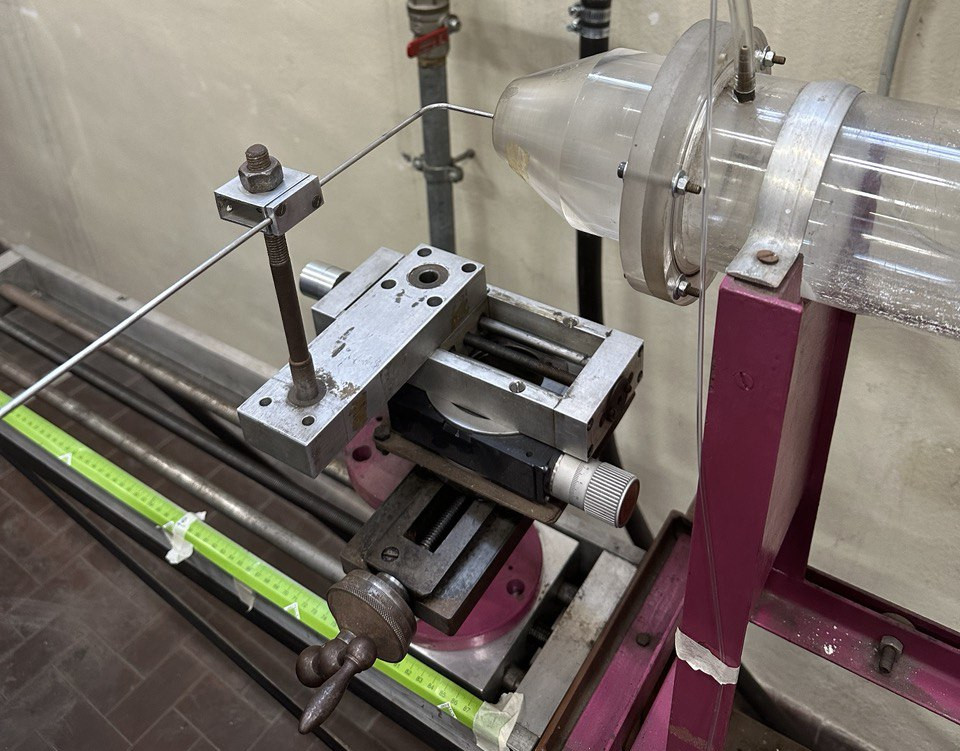
\includegraphics[width=.65\textwidth]{images/2/goniometro.jpg}
    \caption{Goniometro opportunamente posizionato}
\end{figure}

\newpage
\subsection{Procedura sperimentale}
Come prima operazione è necessario misurare la tensione di offset $E_0$, cioè la tensione in uscita al trasduttore quando non è applicata alcuna differenza di pressione. Per fare ciò, si acquisiscono i dati in uscita al trasduttore con il getto spento.\\\\
Una volta misurata tale tensione, si può scomporre il segnale in uscita come:
\begin{equation*}
    E(\Delta p) = E_0 + \Delta E(\Delta p)
\end{equation*}
Si procede mantenendo una portata costante per ogni squadra e quindi una velocità costante nel cuore potenziale del getto e variando l'angolo di disallineamento $\alpha$ in entrambi i versi di rotazione. Per ogni angolo $\alpha$, misurato tramite una scala graduata, si acquisisce il segnale elettrico di uscita corrispondente.\\\\
I dati grezzi acquisiti durante la procedura sono riportati in appendice \ref{a2}.

\subsection{Analisi dati}
L'analisi dati è condotta con l'ausilio di un codice Python, riportato in appendice \ref{b2}.\\\\
Per il calcolo della densità si utilizzano le condizioni di pressione e temperatura ambiente rilevate al momento delle misure, quindi:
\begin{equation*}
    \rho = \frac{p_{amb}}{R\,T_{amb}}
\end{equation*}
In cui $R\approx 287$ è la costante dei gas relativa all'aria.\\\\
Per il calcolo della viscosità dinamica $\mu$ si utilizza la legge di Sutherland:
\begin{equation*}
    \mu = 1.46\cdot10^{-6} \frac{T_{amb}^{3/2}}{T_{amb}+110}
\end{equation*}
Dai dati acquisiti si ricava la pressione dinamica "vera", cioè a disallineamento nullo $q_{\alpha=0}$ per ognuna delle quattro portate analizzate. Da tale grandezza si ricava la velocità:
\begin{equation*}
    V = \sqrt{\frac{2q_{\alpha=0}}{\rho}}
\end{equation*}
E quindi il numero di Reynolds:
\begin{equation*}
    Re = \frac{\rho V D}{\mu}
\end{equation*}
Infine si calcolano gli errori $\varepsilon$ per la pressione statica, la pressione totale e la pressione dinamica, utilizzando le formule precedentemente esplicitate.
\newpage
\noindent Si ottengono i seguenti diagrammi:
\begin{figure}[h!]
    \centering
    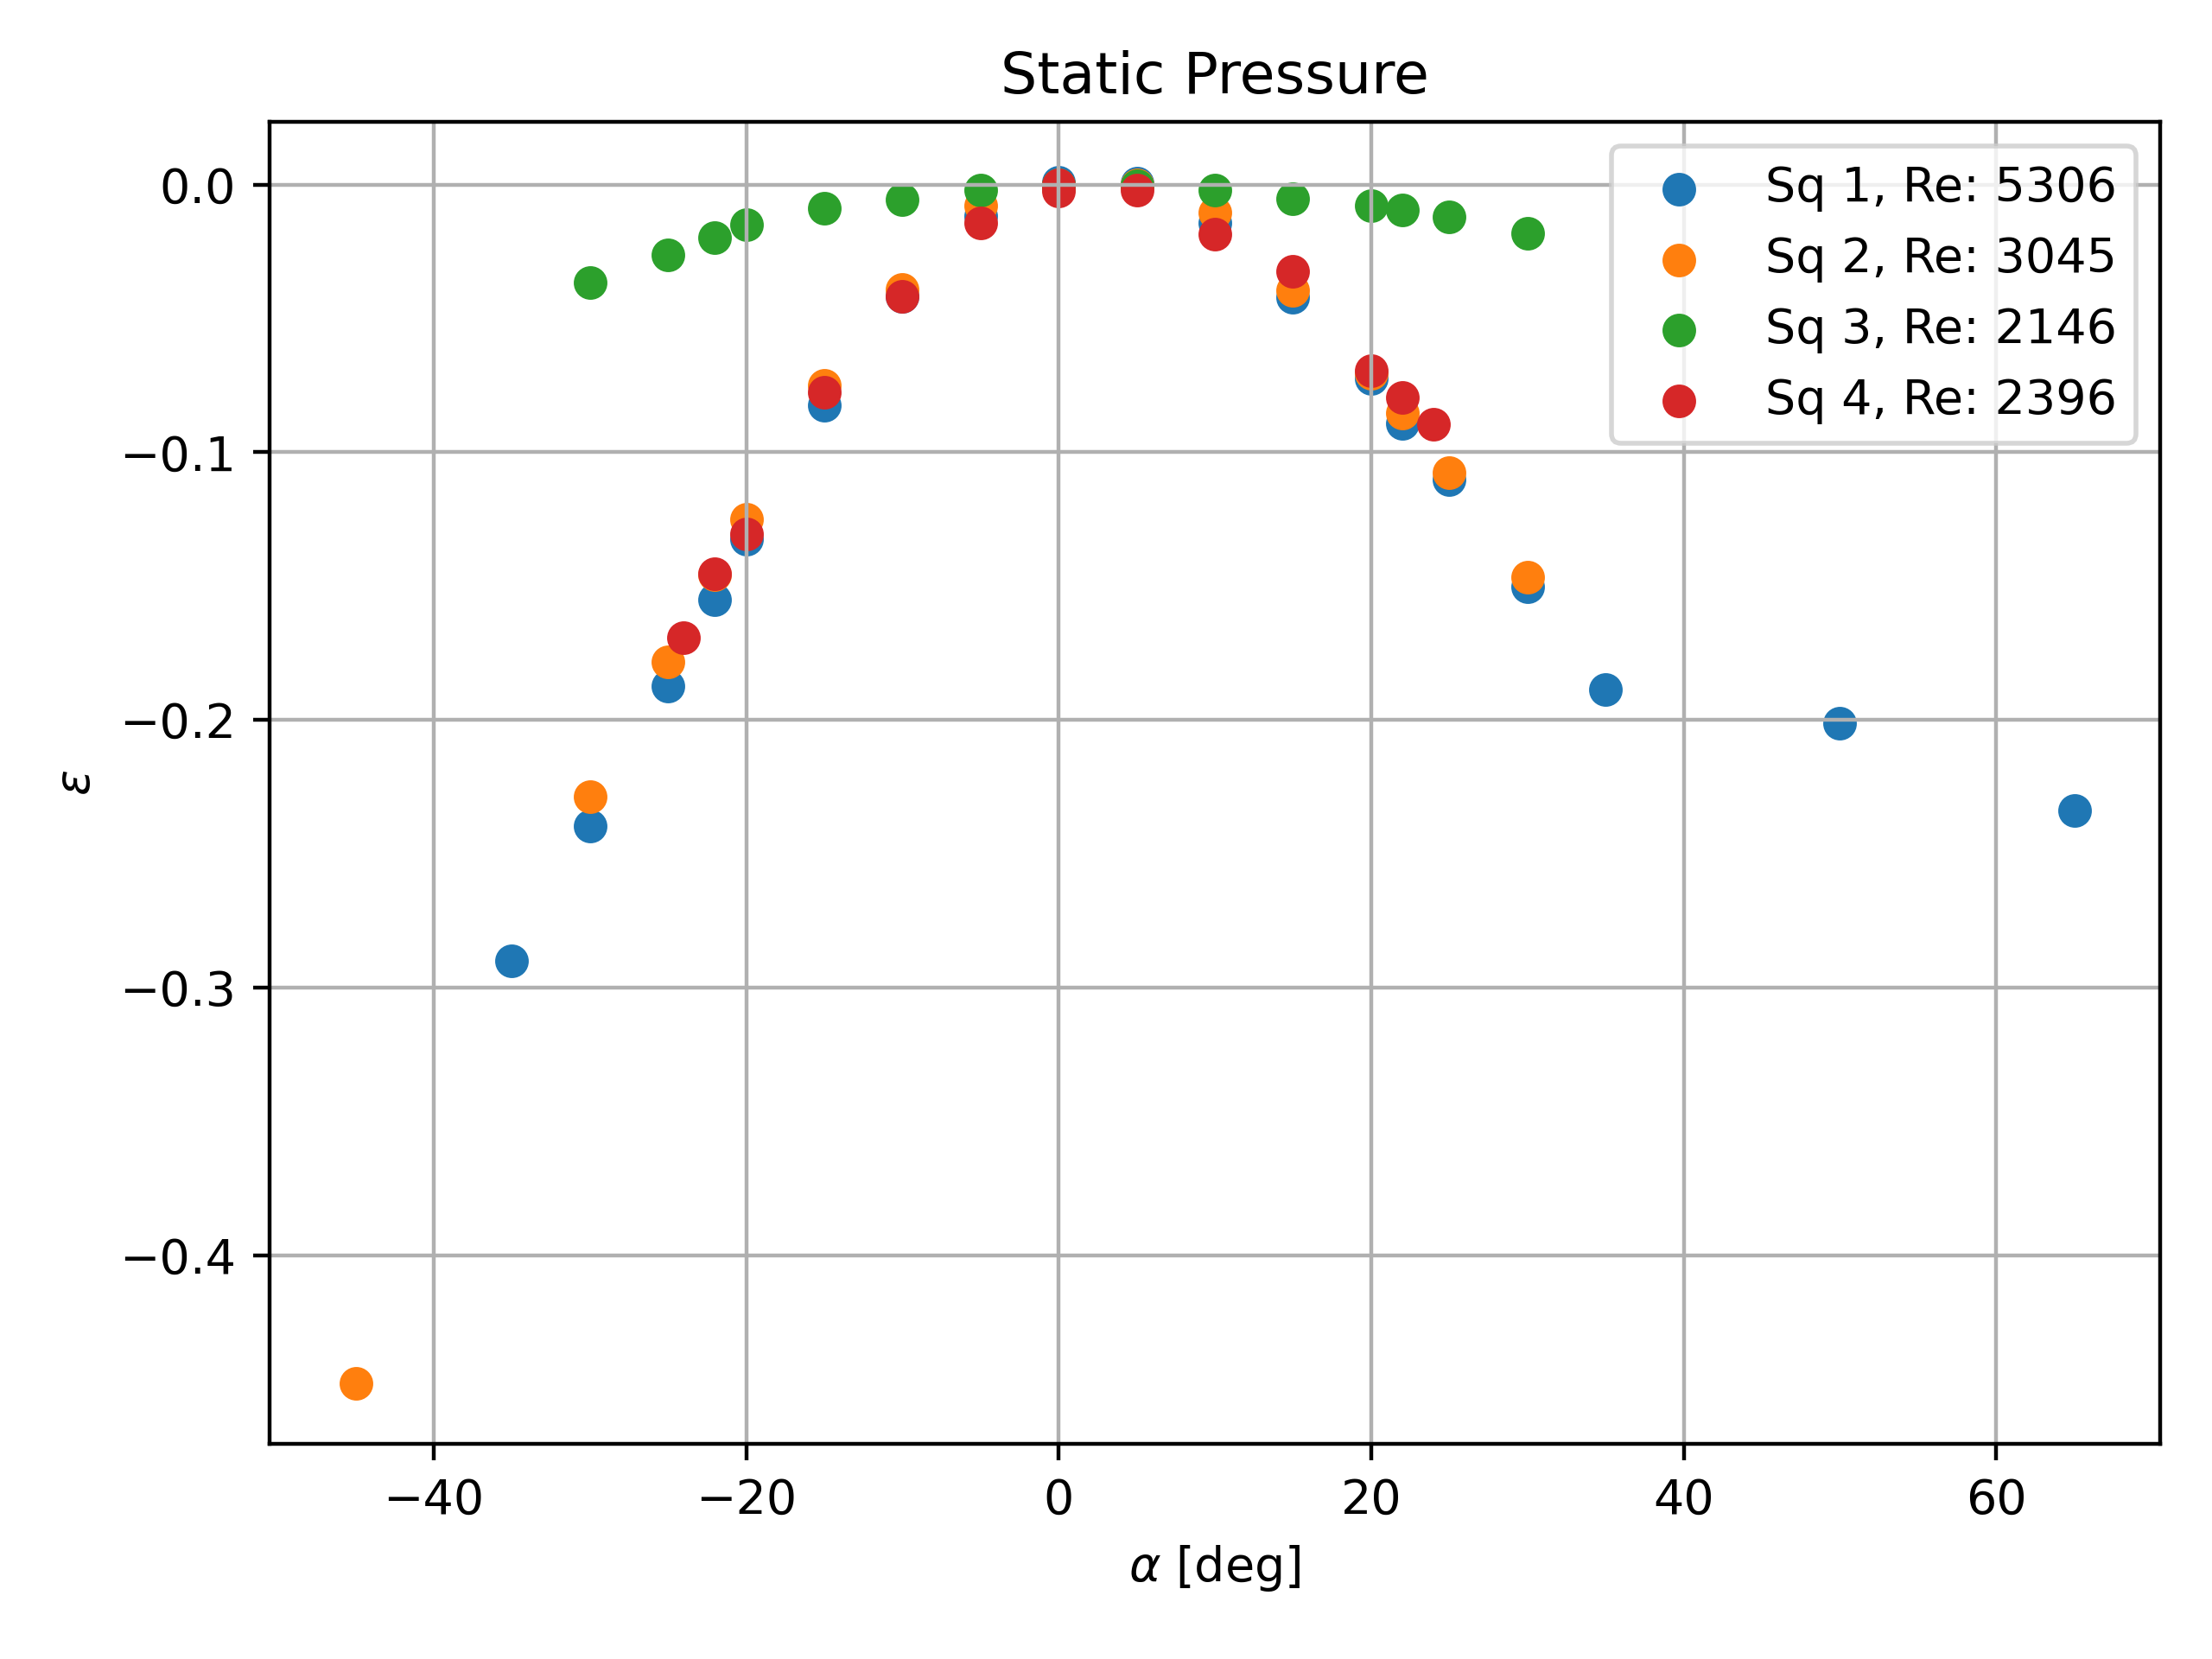
\includegraphics[width=.76\textwidth]{images/2/p.png}
    \caption{Pressione statica}
\end{figure}
\begin{figure}[h!]
    \centering
    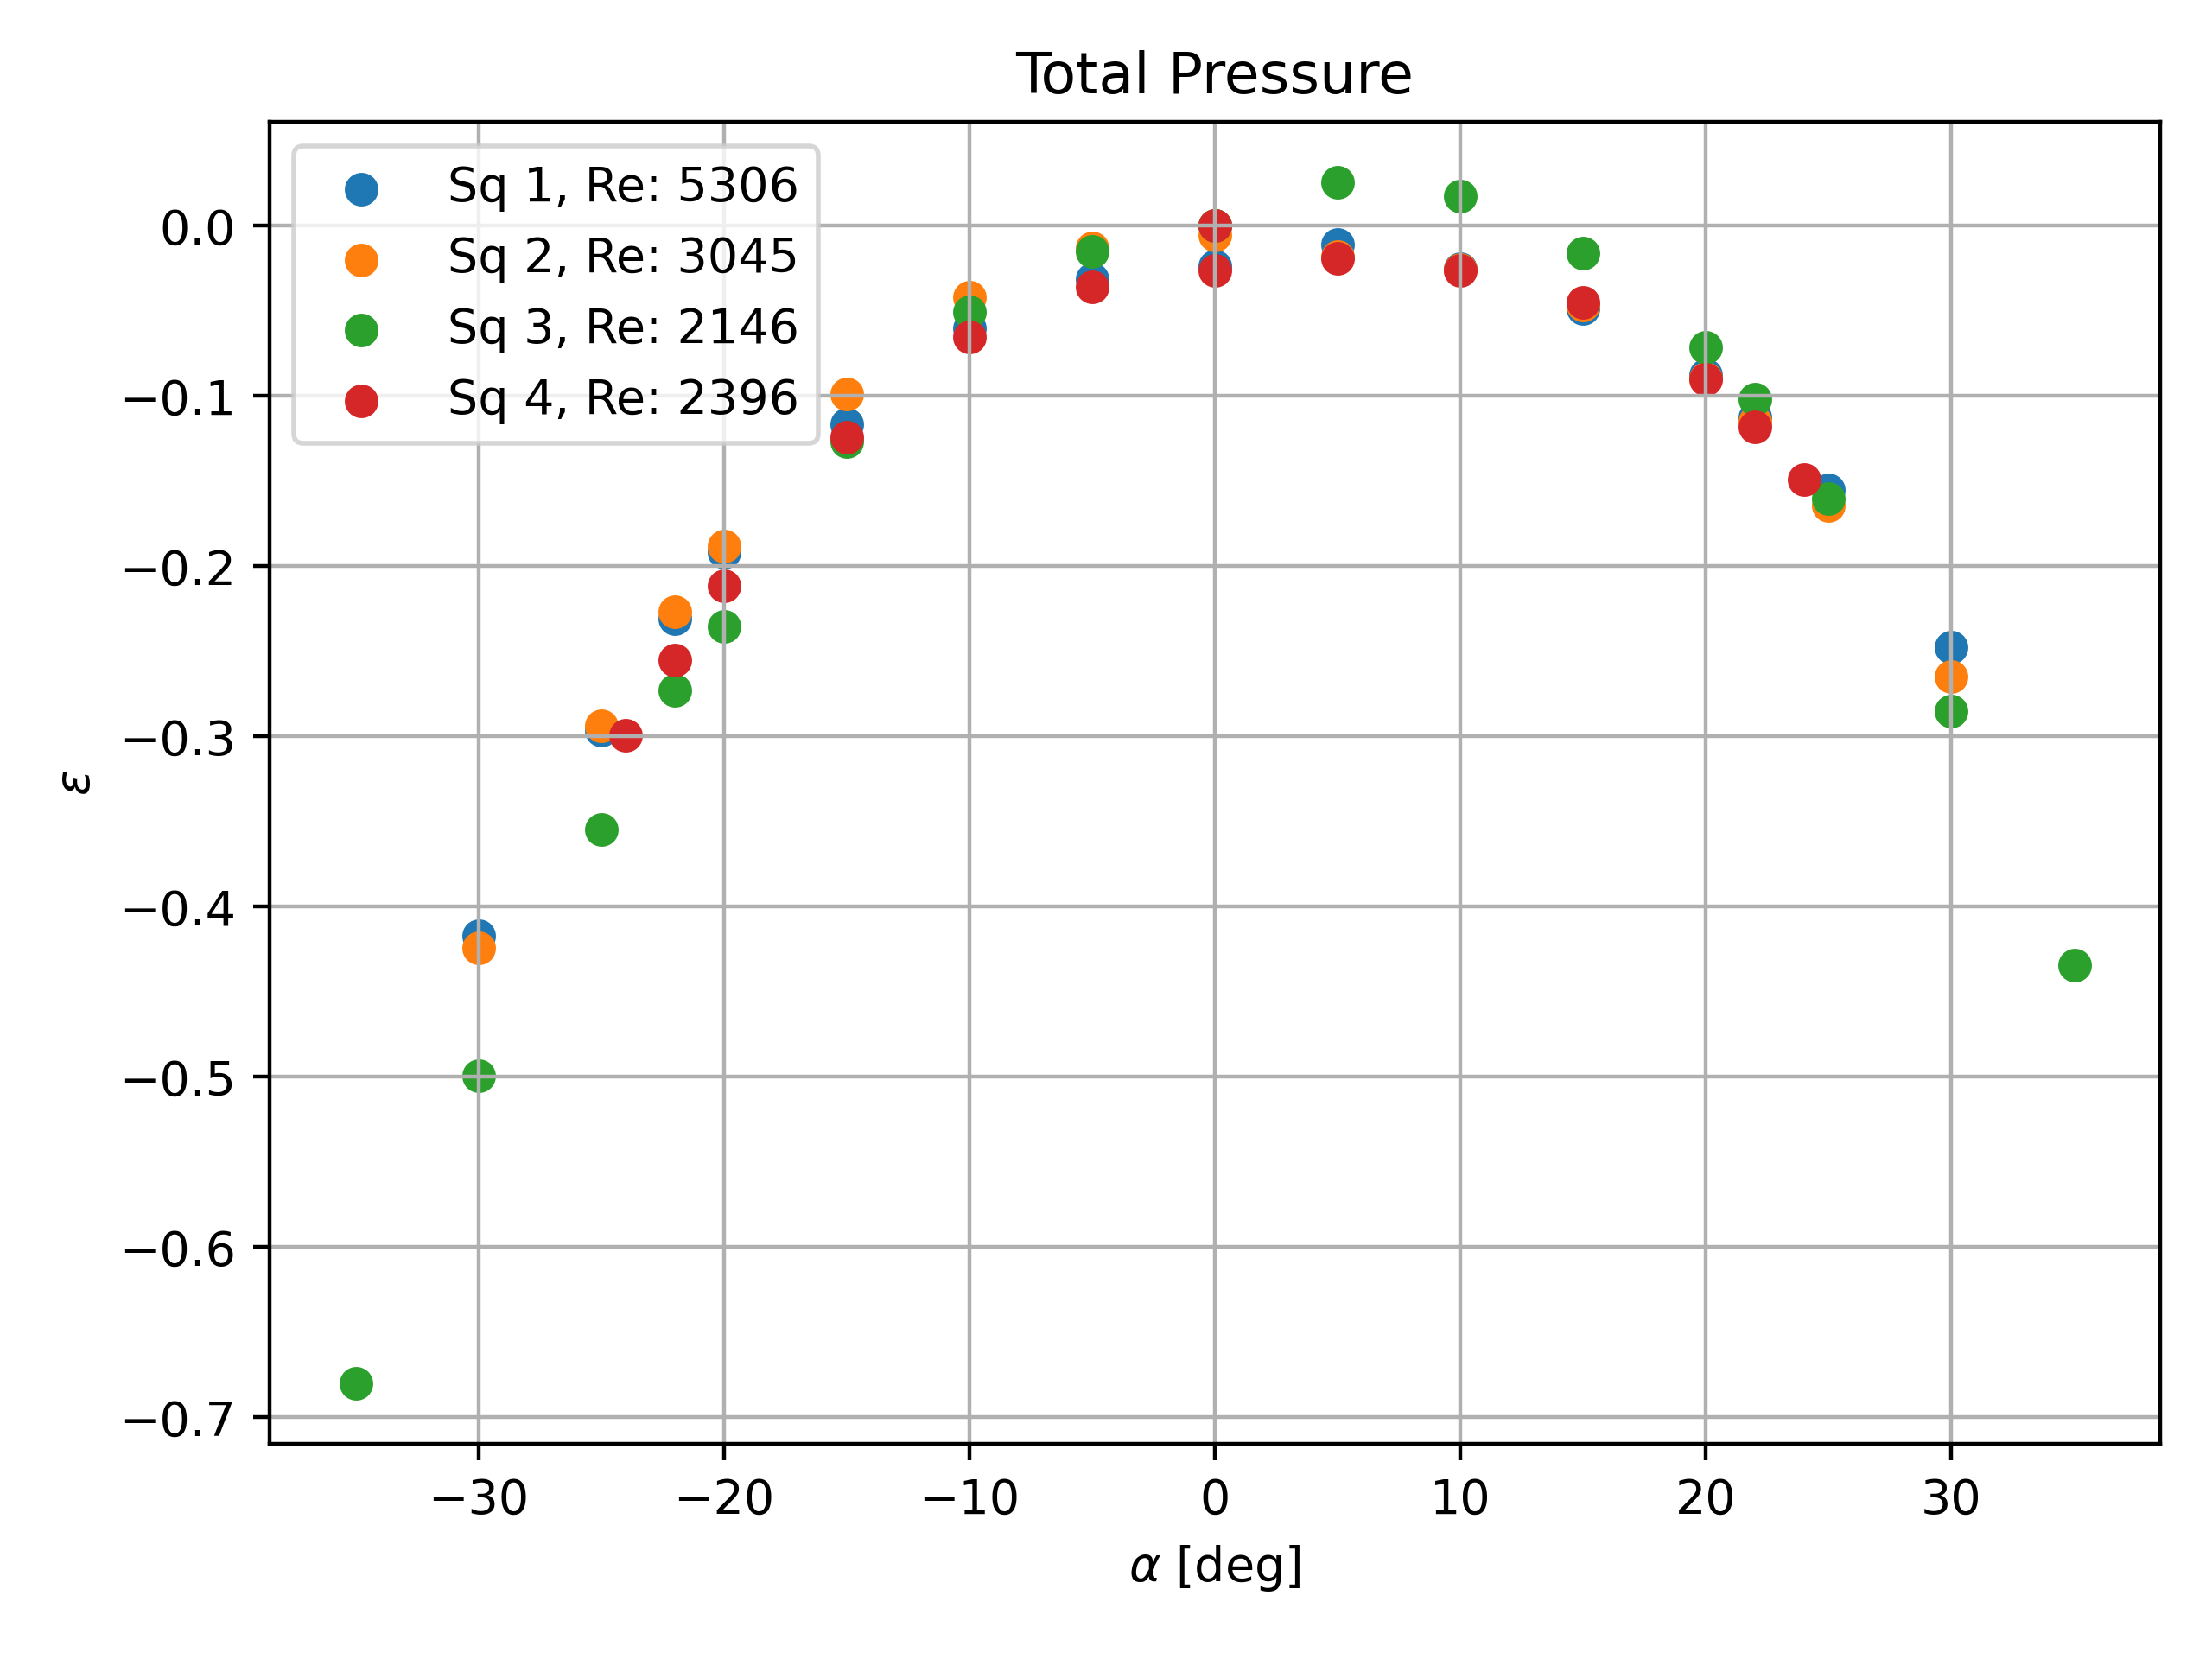
\includegraphics[width=.76\textwidth]{images/2/ptot.png}
    \caption{Pressione totale}
\end{figure}

\newpage
\begin{figure}[ht]
    \centering
    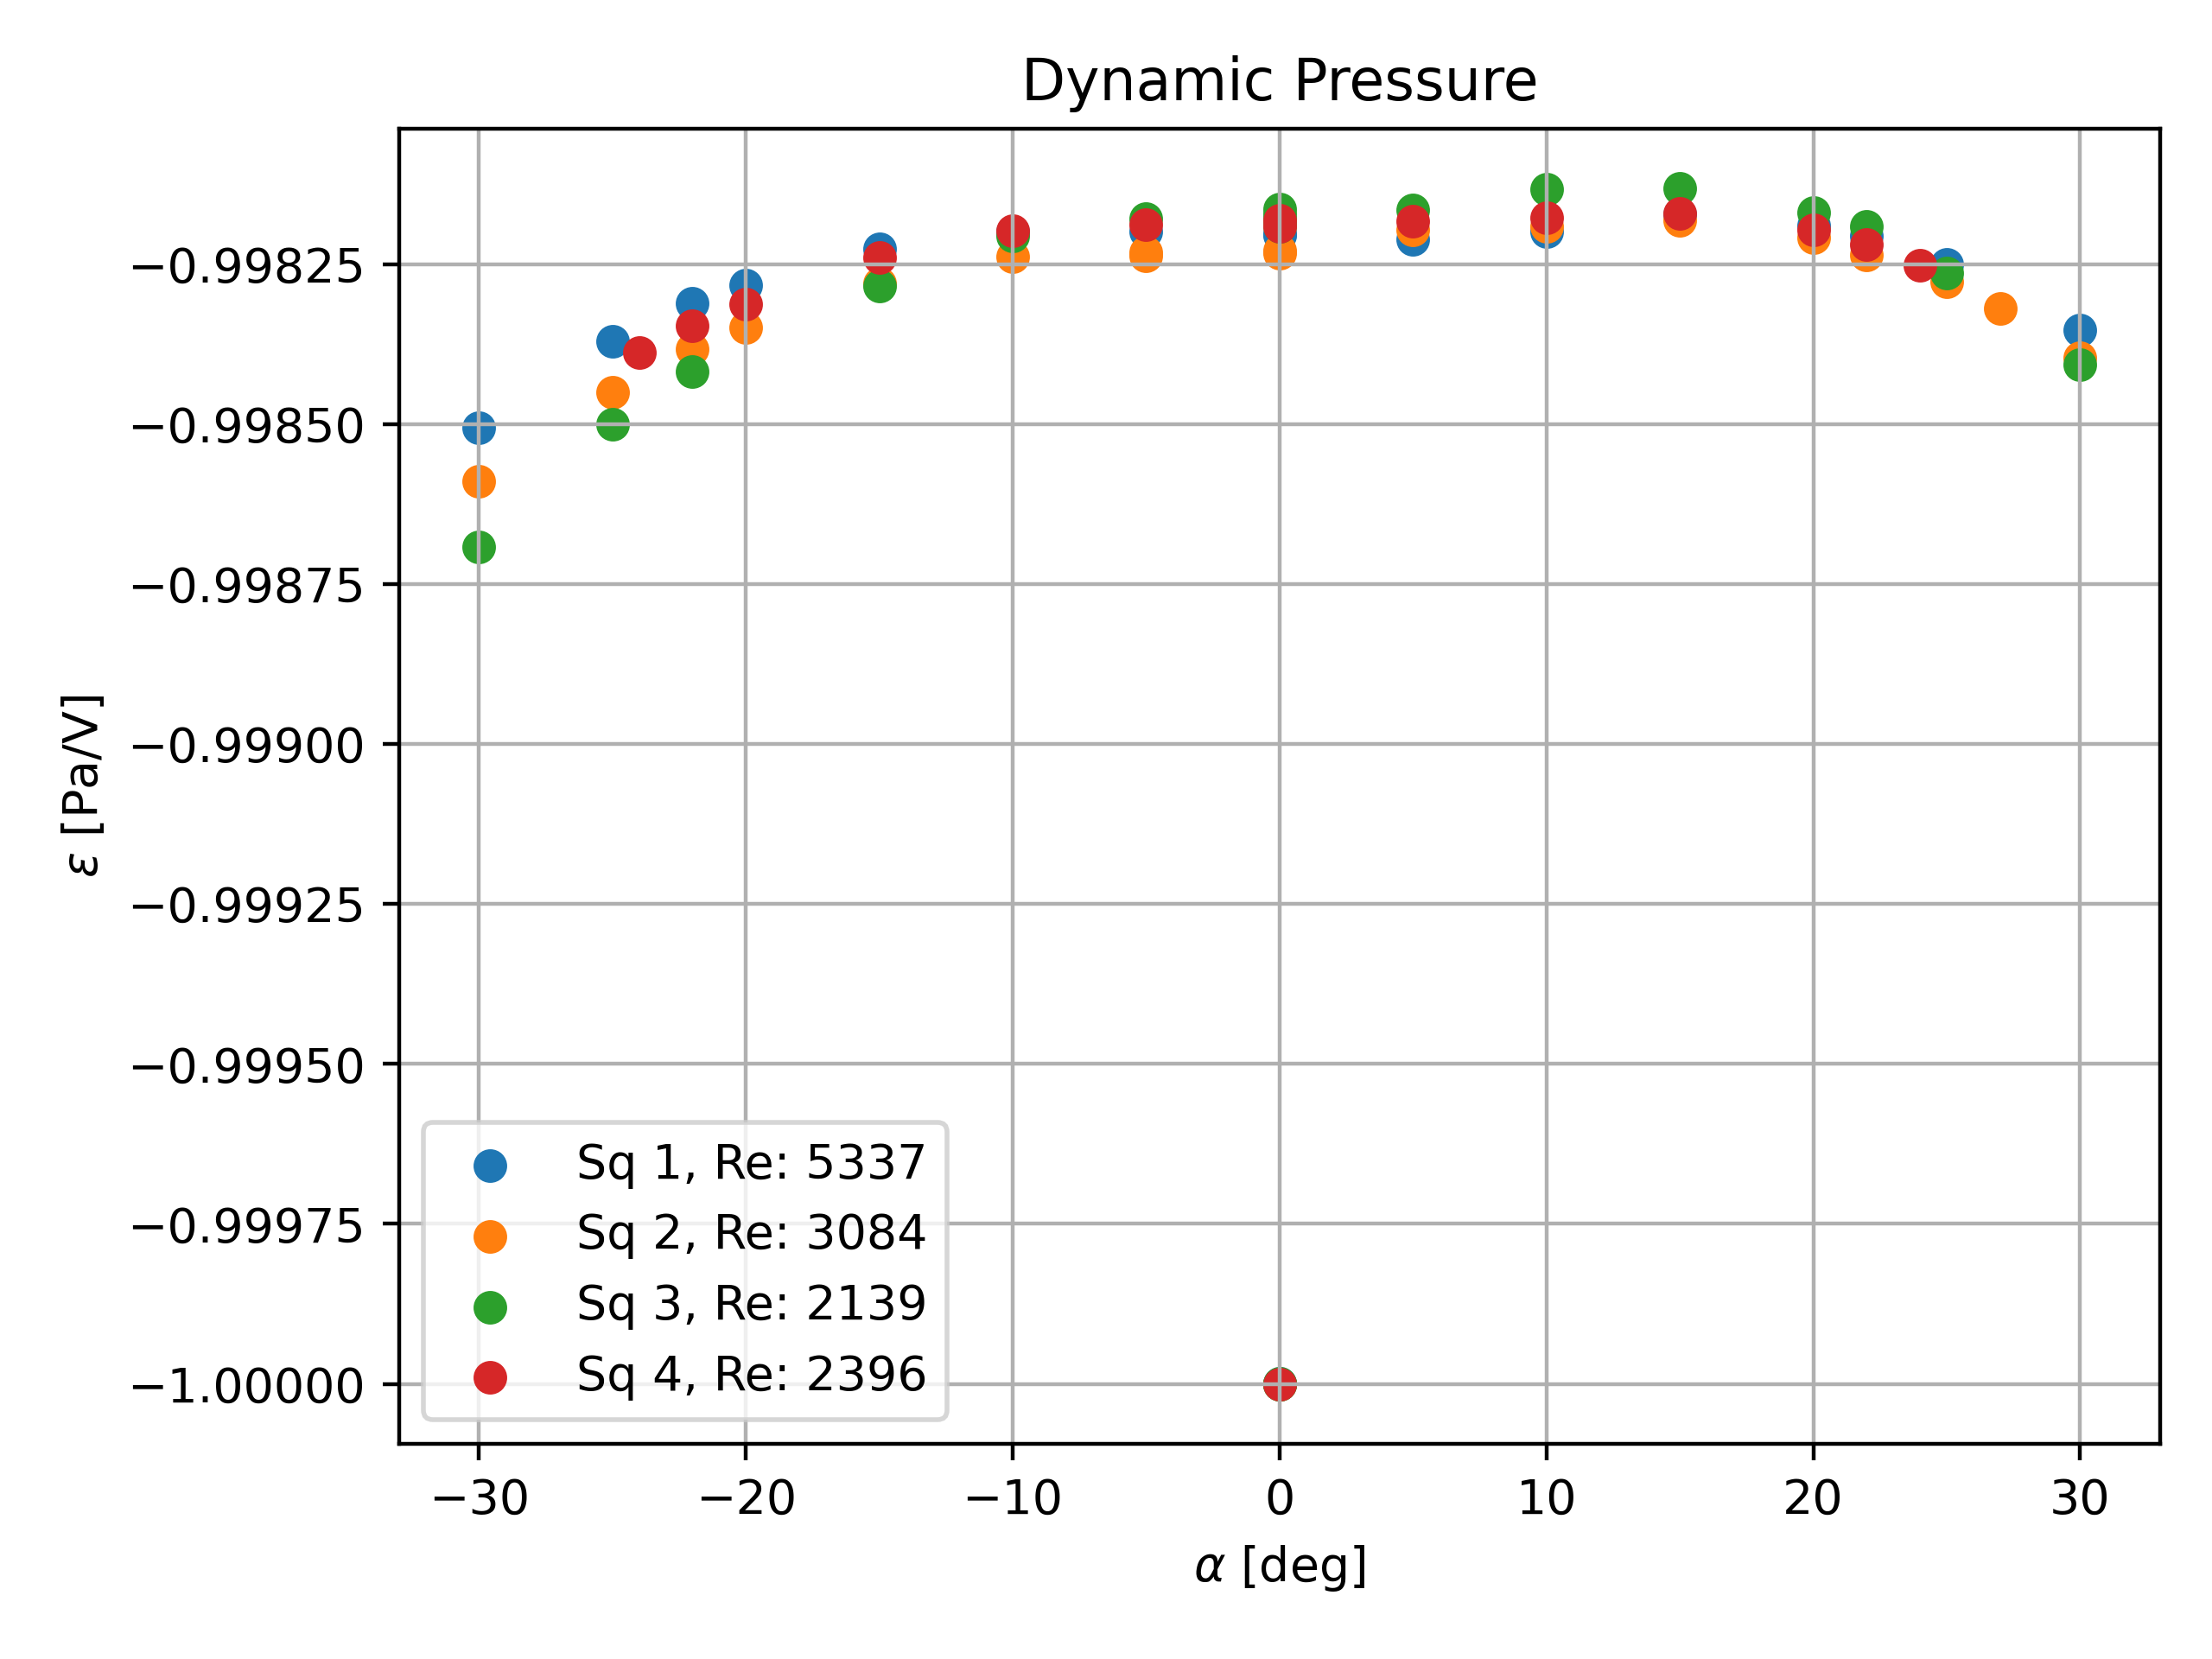
\includegraphics[width=.76\textwidth]{images/2/q.png}
    \caption{Pressione dinamica}
\end{figure}

\noindent I risultati ottenuti corrispondono ai diagrammi presenti in letteratura.\\\\
Si evidenzia la leggera influenza del numero di Reynolds sulle pendenze delle varie curve sperimentali, in particolar modo di quelle relative alla pressione statica.\\\\
L'evidente asimmetria dei risultati, ottenuti variando all'angolo di disallineamento, è attribuibile all'interferenza dovuta al gambo della sonda di Pitot. Per ovviare a tale problematica sarebbe stato sufficiente orientare il gambo della sonda in direzione normale al piano di rotazione.

\newpage
\subsection{Tempo caratteristico}
A differenza dell'esercitazione precedente, nell'attuale catena di misura non è presente il manometro di Betz, che operava da collo di bottiglia per la risposta in frequenza della linea pneumatica. Pertanto, è opportuno indagare il fenomeno transitorio della linea pneumatica ed il relativo tempo caratteristico $\tau$.\\\\
Per fare ciò, sono acquisite le tensioni di uscita dal trasduttore con una frequenza di campionamento $f_{samp}=500$ Hz per un periodo $T$ di 2 minuti.\\\\
Per determinare il tempo caratteristico si interpolano i dati sperimentali con una curva esponenziale, del tipo:
\begin{equation*}
    E(t) = Ae^{bt} = Ae^{-\frac t\tau}
\end{equation*}
Maneggiando tale relazione, si ottiene:
\begin{equation*}
    \log E(t) = \log A + bt = c_1 t + c_2 \quad \Rightarrow \quad b = -\frac1\tau = c_1 \ ; \ A = e^{c_2}
\end{equation*}
Si ricava dunque il tempo caratteristico della linea pneumatica:
\begin{equation*}
    \tau = 0.400\ \text{s}
\end{equation*}
\begin{figure}[H]
    \centering
    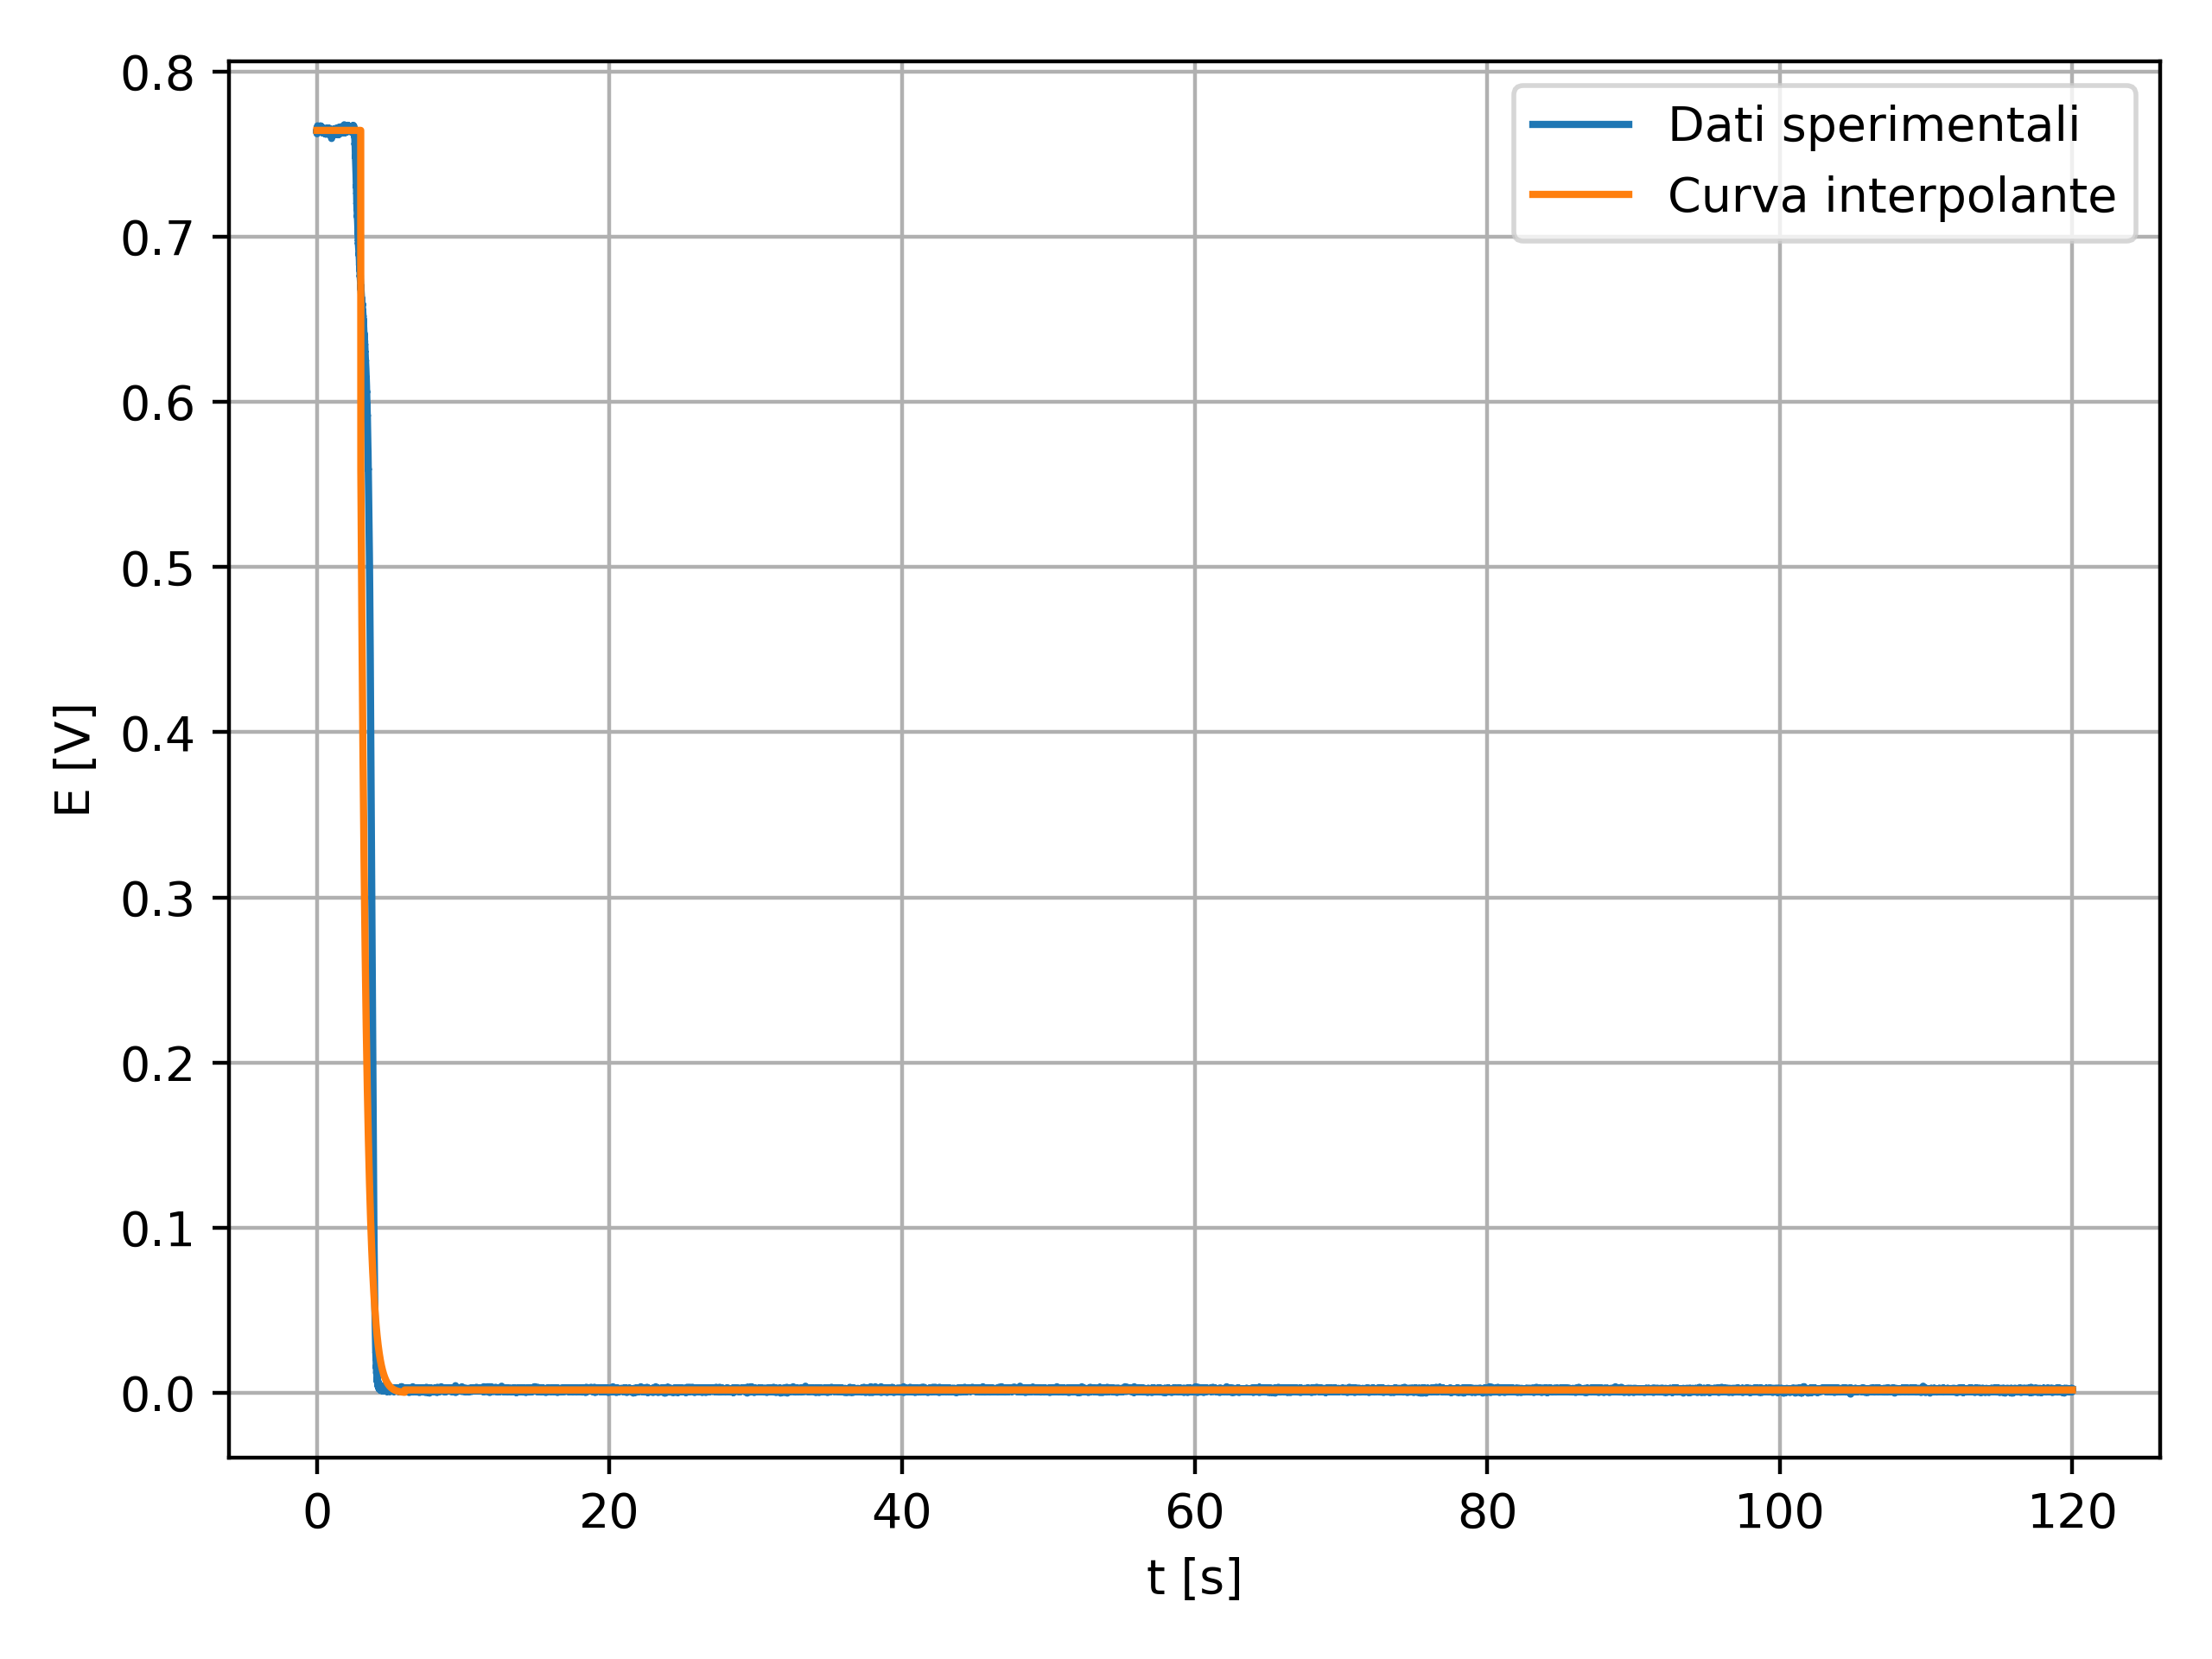
\includegraphics[width=.9\textwidth]{images/2/transitorio.png}
    \caption{Transitorio relativo alla pressione dinamica $q(t)$}\label{fig:t2}
\end{figure}
\section{Struttura del getto}
Il getto è un flusso libero caratterizzato da effetti viscosi. Rientra nei cosiddetti free shear flows a cui fanno capo anche le scie e i mixing layer.\\\\
Il getto si origina quando una data portata di fluido fuoriesce da un orifizio. Se l'orifizio è caratterizzato da una geometria circolare, il getto è detto assialsimmetrico.
\begin{figure}[h]
    \centering
    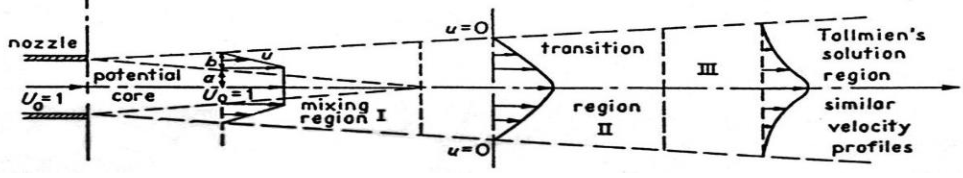
\includegraphics[width=0.95\linewidth]{images/3/getto.png}
    \caption{Rappresentazione dei campi caratteristici di un getto}
\end{figure}

\noindent A partire dalla sezione di uscita vengono a generarsi ed a svilupparsi diverse regioni caratteristiche all'interno di un getto turbolento. In prossimità dell'orifizio si genera una zona conica a velocità costante detta cuore potenziale. Questa zona è delimitata da una mixing region, dove il flusso potenziale si miscela con il flusso circostante. Tale zona è seguita da una zona di transizione ed infine da una zona autosimilare.\\\\
Nella regione autisimilare (o self-similar) il getto evolve rallentando e allargandosi. La peculiarità di questa regione è che i profili di velocità, pur variando in termini assoluti, sono costanti in termini adimensionali purché la normalizzazione venga eseguita in termini di velocità massima e dimensione trasversale del getto locali.

\subsection{Descrizione dell'esperimento}
La presente esercitazione si pone come obiettivo la caratterizzazione della struttura di un getto assialsimmetrico turbolento. Si vuole quindi misurare la velocità media e le fluttuazioni di velocità all'interno del getto, al variare della posizione assiale $x$, della posizione trasversale $r$ e del numero di Reynolds.

\subsection{Catena di misura}
Per misurare la velocità si utilizza un tubo di Pitot, le cui uscite sono collegate al trasduttore di pressione differenziale precedentemente tarato.\\\\
Al fine di misurare la velocità in più punti nello spazio è necessario dotare la catena di misura di alcuni posizionatori. In particolare, il tubo di Pitot è montato su due diverse slitte ortogonali, una che permette il movimento nella direzione assiale e l'altra che permette il movimento nella direzione trasversale.\\\\
La catena di misura è dunque costituita da:
\begin{itemize}
    \item Getto;
    \item Tubo di Pitot;
    \item Posizionatori della sonda di Pitot;
    \item Trasduttore di pressione;
    \item Sistema di acquisizione dati (SAD) e PC con LabView.
\end{itemize}
\begin{figure}[H]
    \centering
    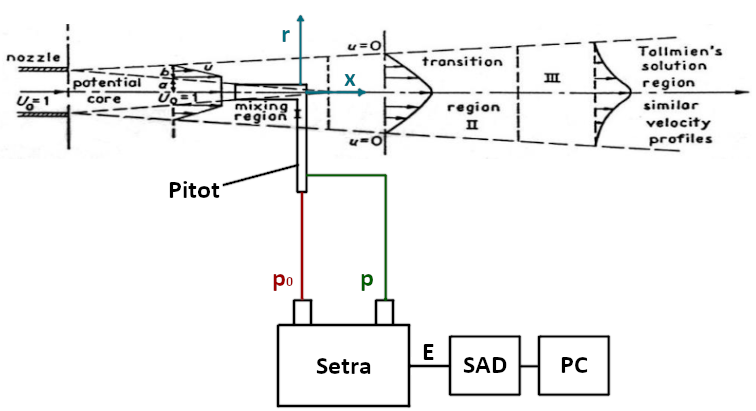
\includegraphics[width=.85\textwidth]{images/3/catena.png}
    \caption{Catena di misura}
\end{figure}
\begin{figure}[H]
    \centering
    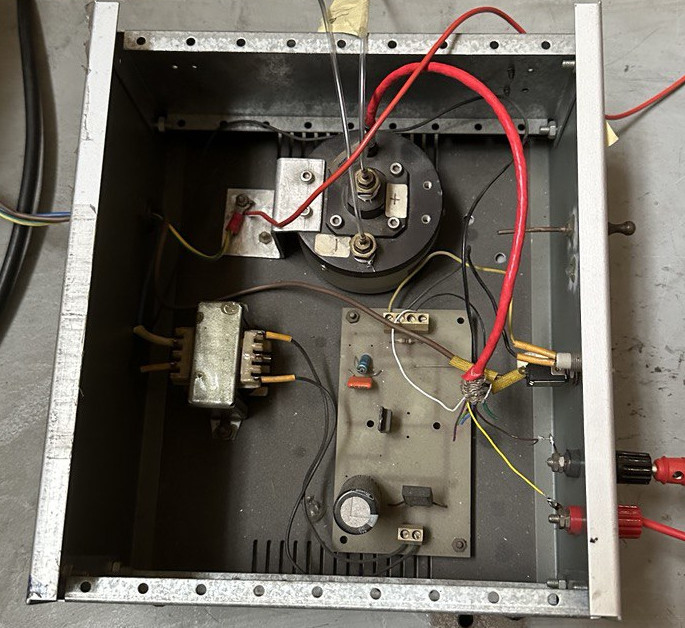
\includegraphics[width=.5\textwidth]{images/3/trasd.jpg}
    \caption{Trasduttore di pressione}
\end{figure}
\begin{figure}[ht]
    \centering
    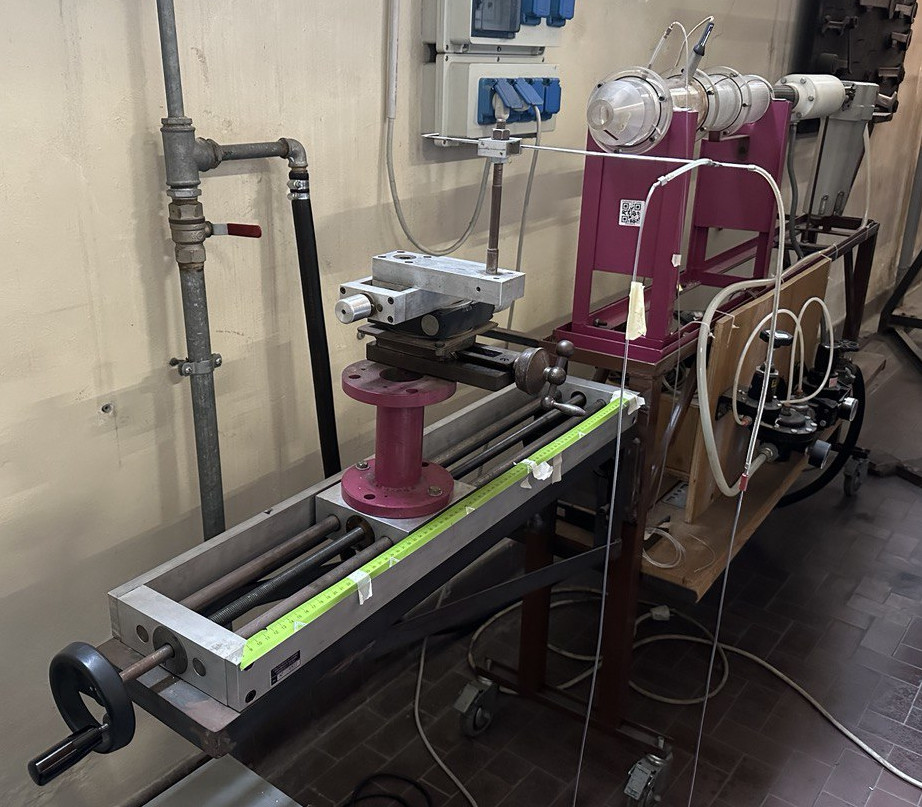
\includegraphics[width=.85\textwidth]{images/3/gettomanopole.jpg}
    \caption{Sistema di posizionamento della sonda di Pitot}
\end{figure}

\subsection{Procedimento operativo}
Ogni squadra effettua misure per una portata costante. Pertanto si ricavano dati per quattro diversi valori di portata, quindi quattro diversi numeri di Reynolds.\\\\
Le misure sono effettuate al variare della distanza trasversale del getto $r$ e per diversi valori di distanza assiale $x$.\\\\
Per regolare la distanza trasversale e la distanza assiale, sono presenti due diverse manopole. Il primo passo consiste nel misurare l'attuale distanza assiale con l'utilizzo di un metro. Una volta definita la distanza assiale, si procede a far variare la distanza trasversale in entrambi i versi rispetto all'asse del getto e si acquisiscono i dati in uscita dal trasduttore di pressione. Una volta acquisiti sufficienti misurazioni si passa ad una diversa distanza assiale $x$ e si ripete la procedura di acquisizione dati.\\\\
I dati grezzi acquisiti mediante questa procedura sono riportati in appendice \ref{a3}.

\subsection{Analisi dati}
L'analisi dati è condotta con l'ausilio di un codice Python, riportato in appendice \ref{b3}.\\\\
Come prima cosa si utilizzano i valori di pressione e temperatura ambiente per determinare la densità e la viscosità dinamica dell'aria:
\begin{equation*}
    \rho = \frac{p_{amb}}{R T_{amb}} \qquad \mu = 1.46\cdot10^{-6} \frac{T_{amb}^{3/2}}{T_{amb}+110}
\end{equation*}
Successivamente si misura la tensione di offset del trasduttore $E_0$, così da poter scomporre il segnale di tensione in uscita come segue:
\begin{equation*}
    E = E_0 + \Delta E
\end{equation*}
Dalle tensioni in uscita acquisite, si calcola la pressione dinamica e quindi la velocità:
\begin{equation*}
    q = \frac12 \rho U^2 = K_t \Delta E = K_t (E - E_0) \quad \Rightarrow \quad U = \sqrt{\frac{2q}\rho}
\end{equation*}
Si può quindi diagrammare l'andamento della velocità in funzione della posizione trasversale $r$ ed assiale $x$:
\begin{figure}[h]
    \centering
    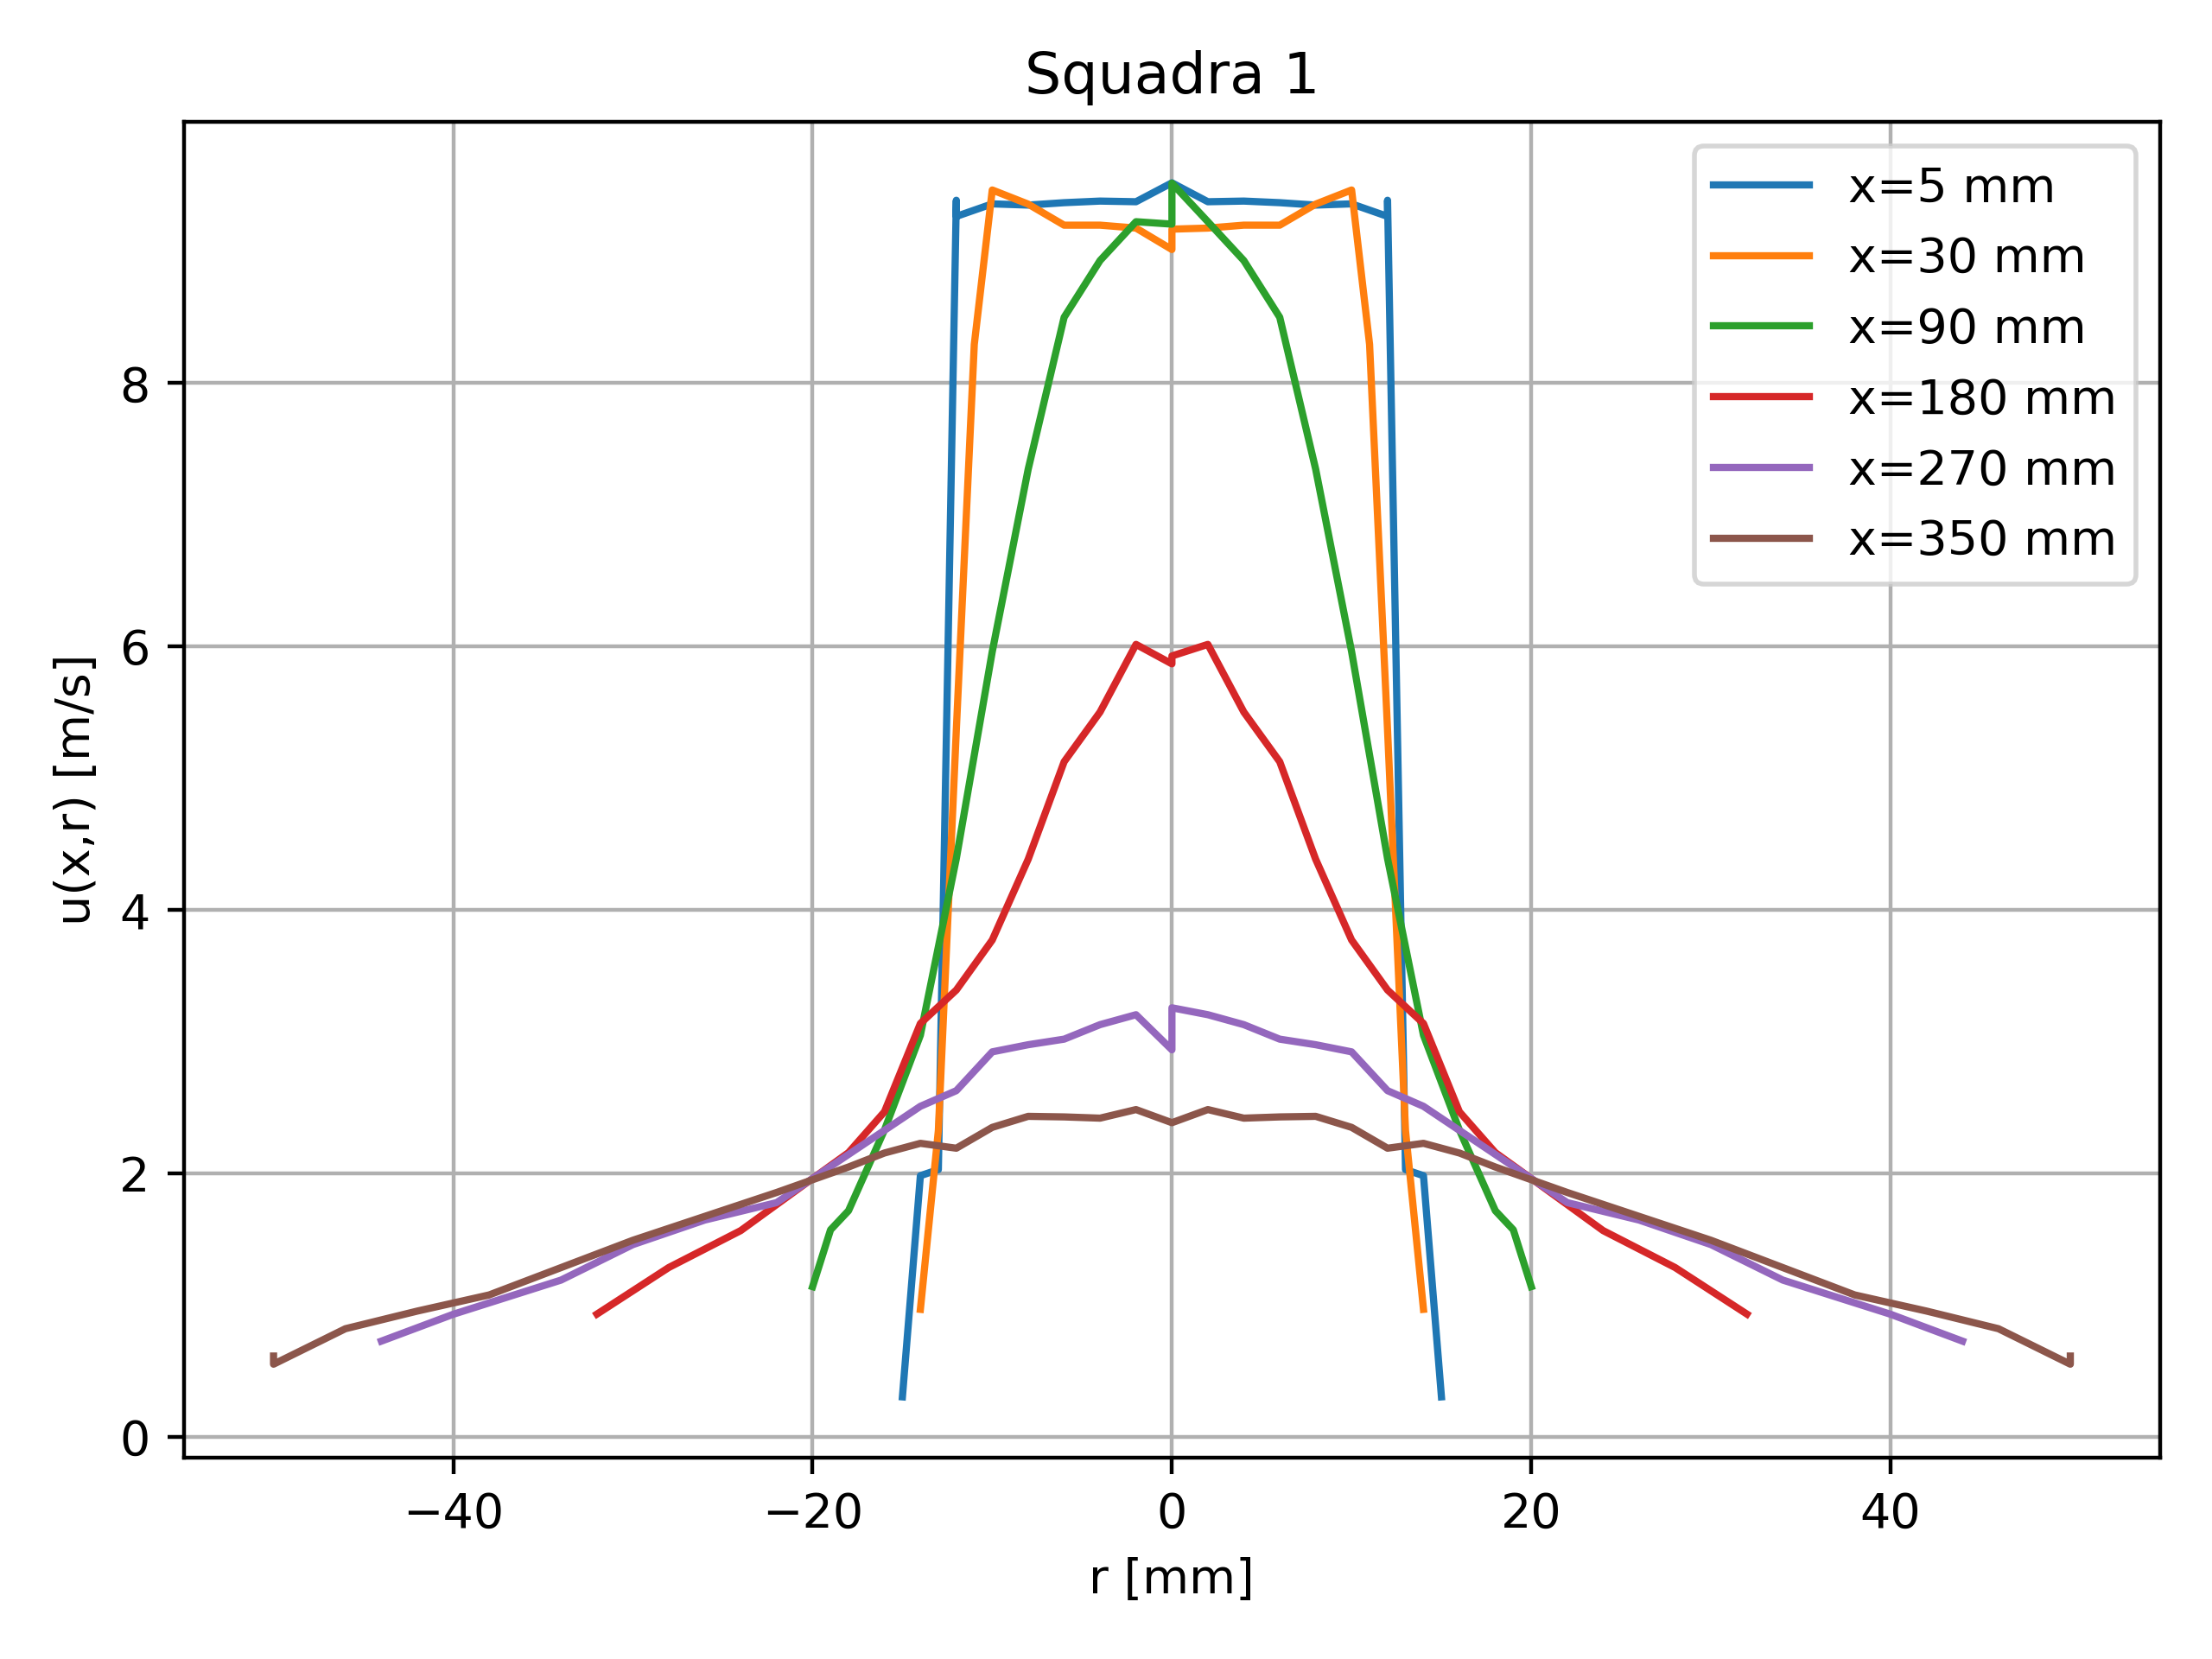
\includegraphics[width=.9\textwidth]{images/3/sq1.png}
    \caption{Profili di velocità per la prima squadra}
\end{figure}
\begin{figure}[ht]
    \centering
    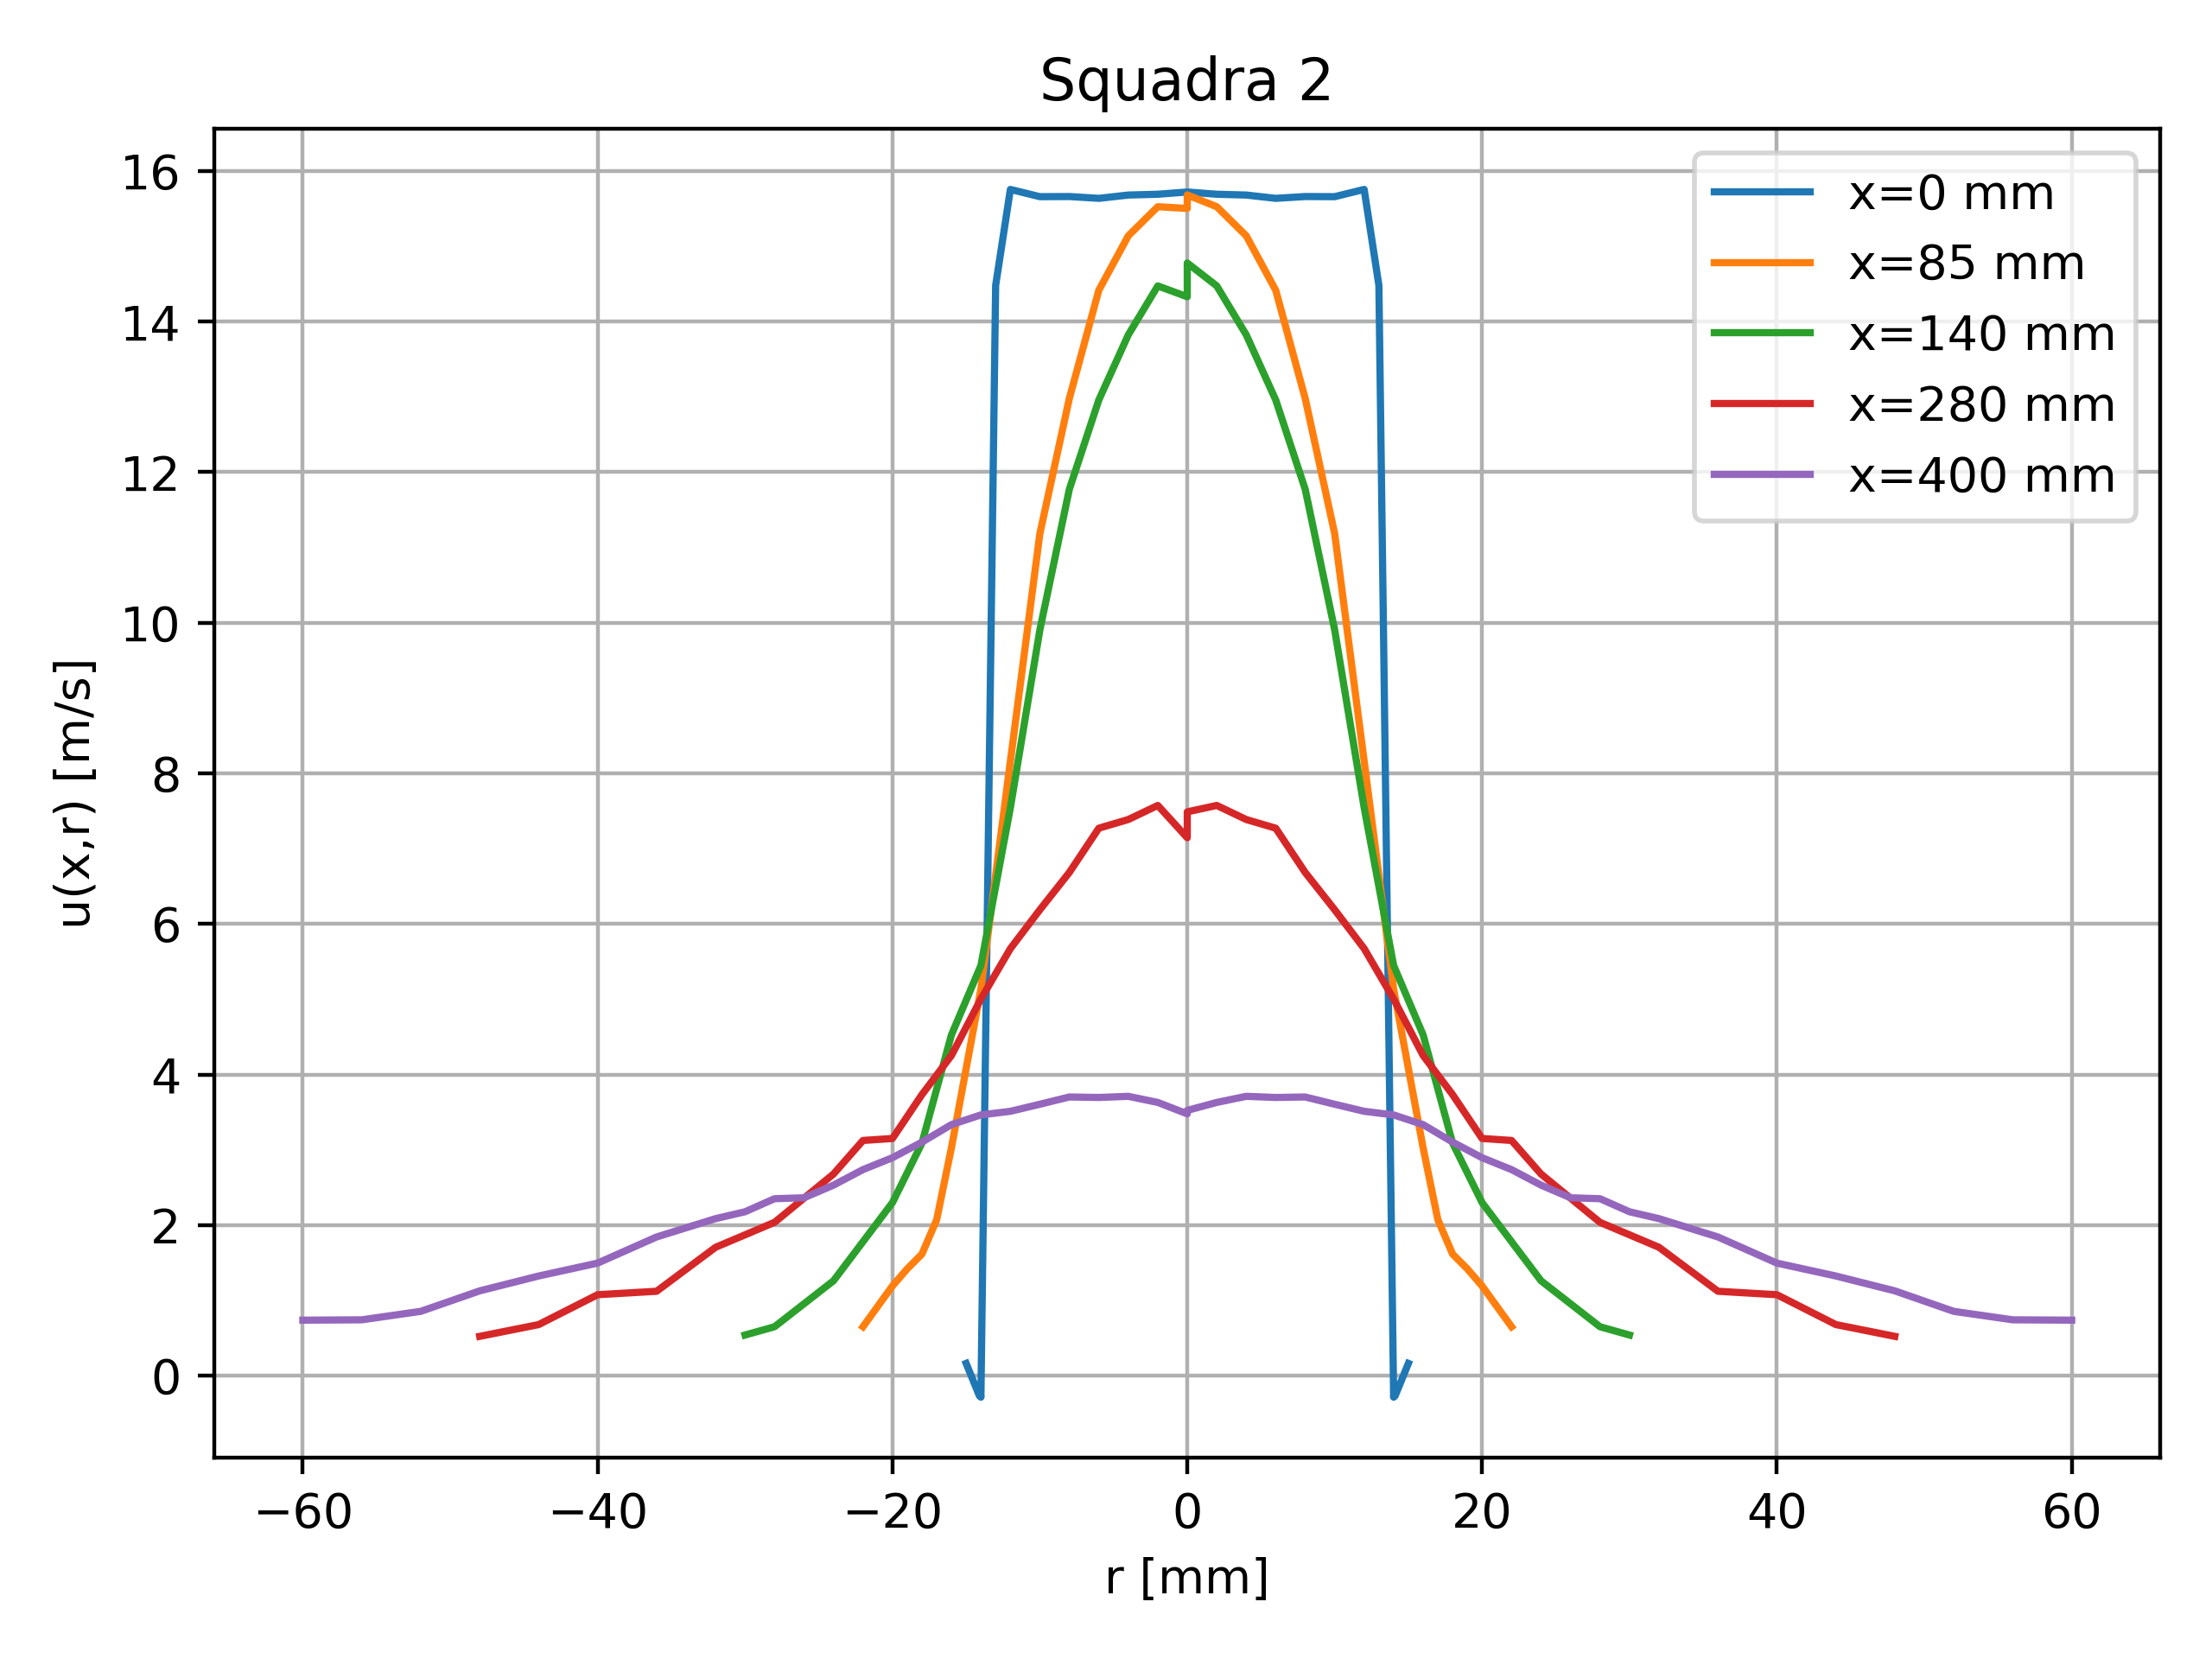
\includegraphics[width=.85\textwidth]{images/3/sq2.png}
    \caption{Profili di velocità per la seconda squadra}
\end{figure}
\begin{figure}[H]
    \centering
    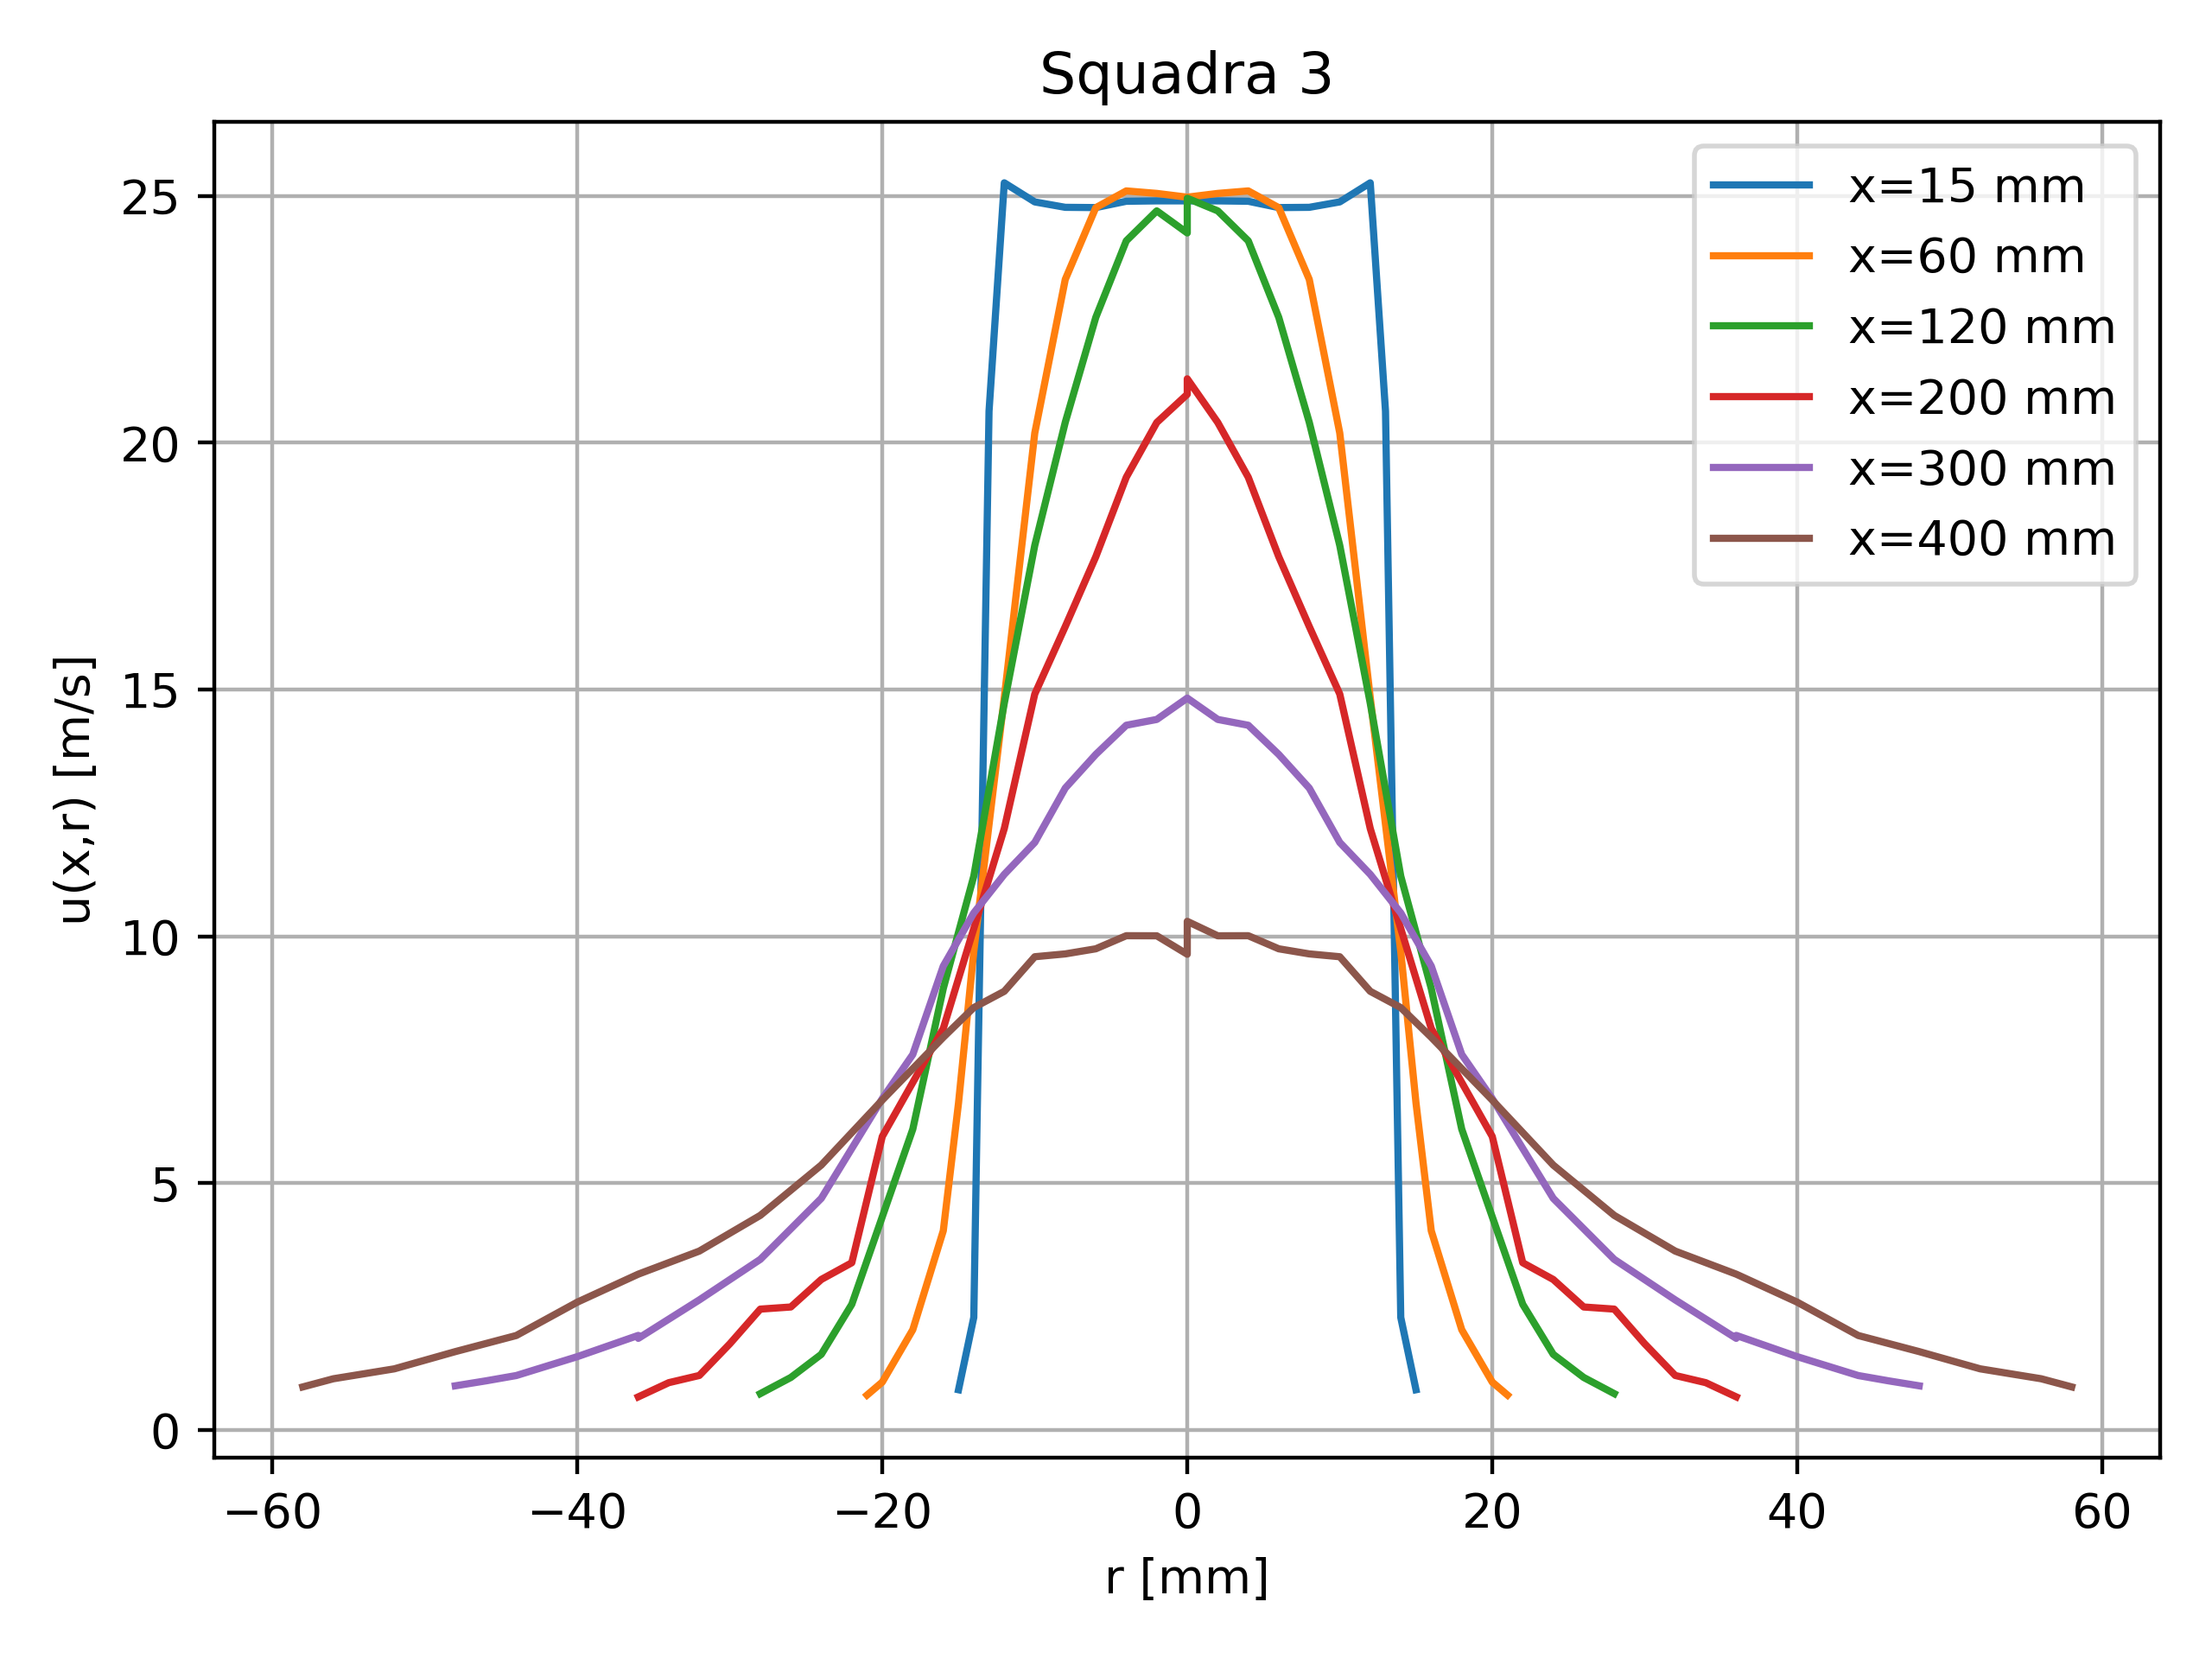
\includegraphics[width=.85\textwidth]{images/3/sq3.png}
    \caption{Profili di velocità per la terza squadra}
\end{figure}
\begin{figure}[ht]
    \centering
    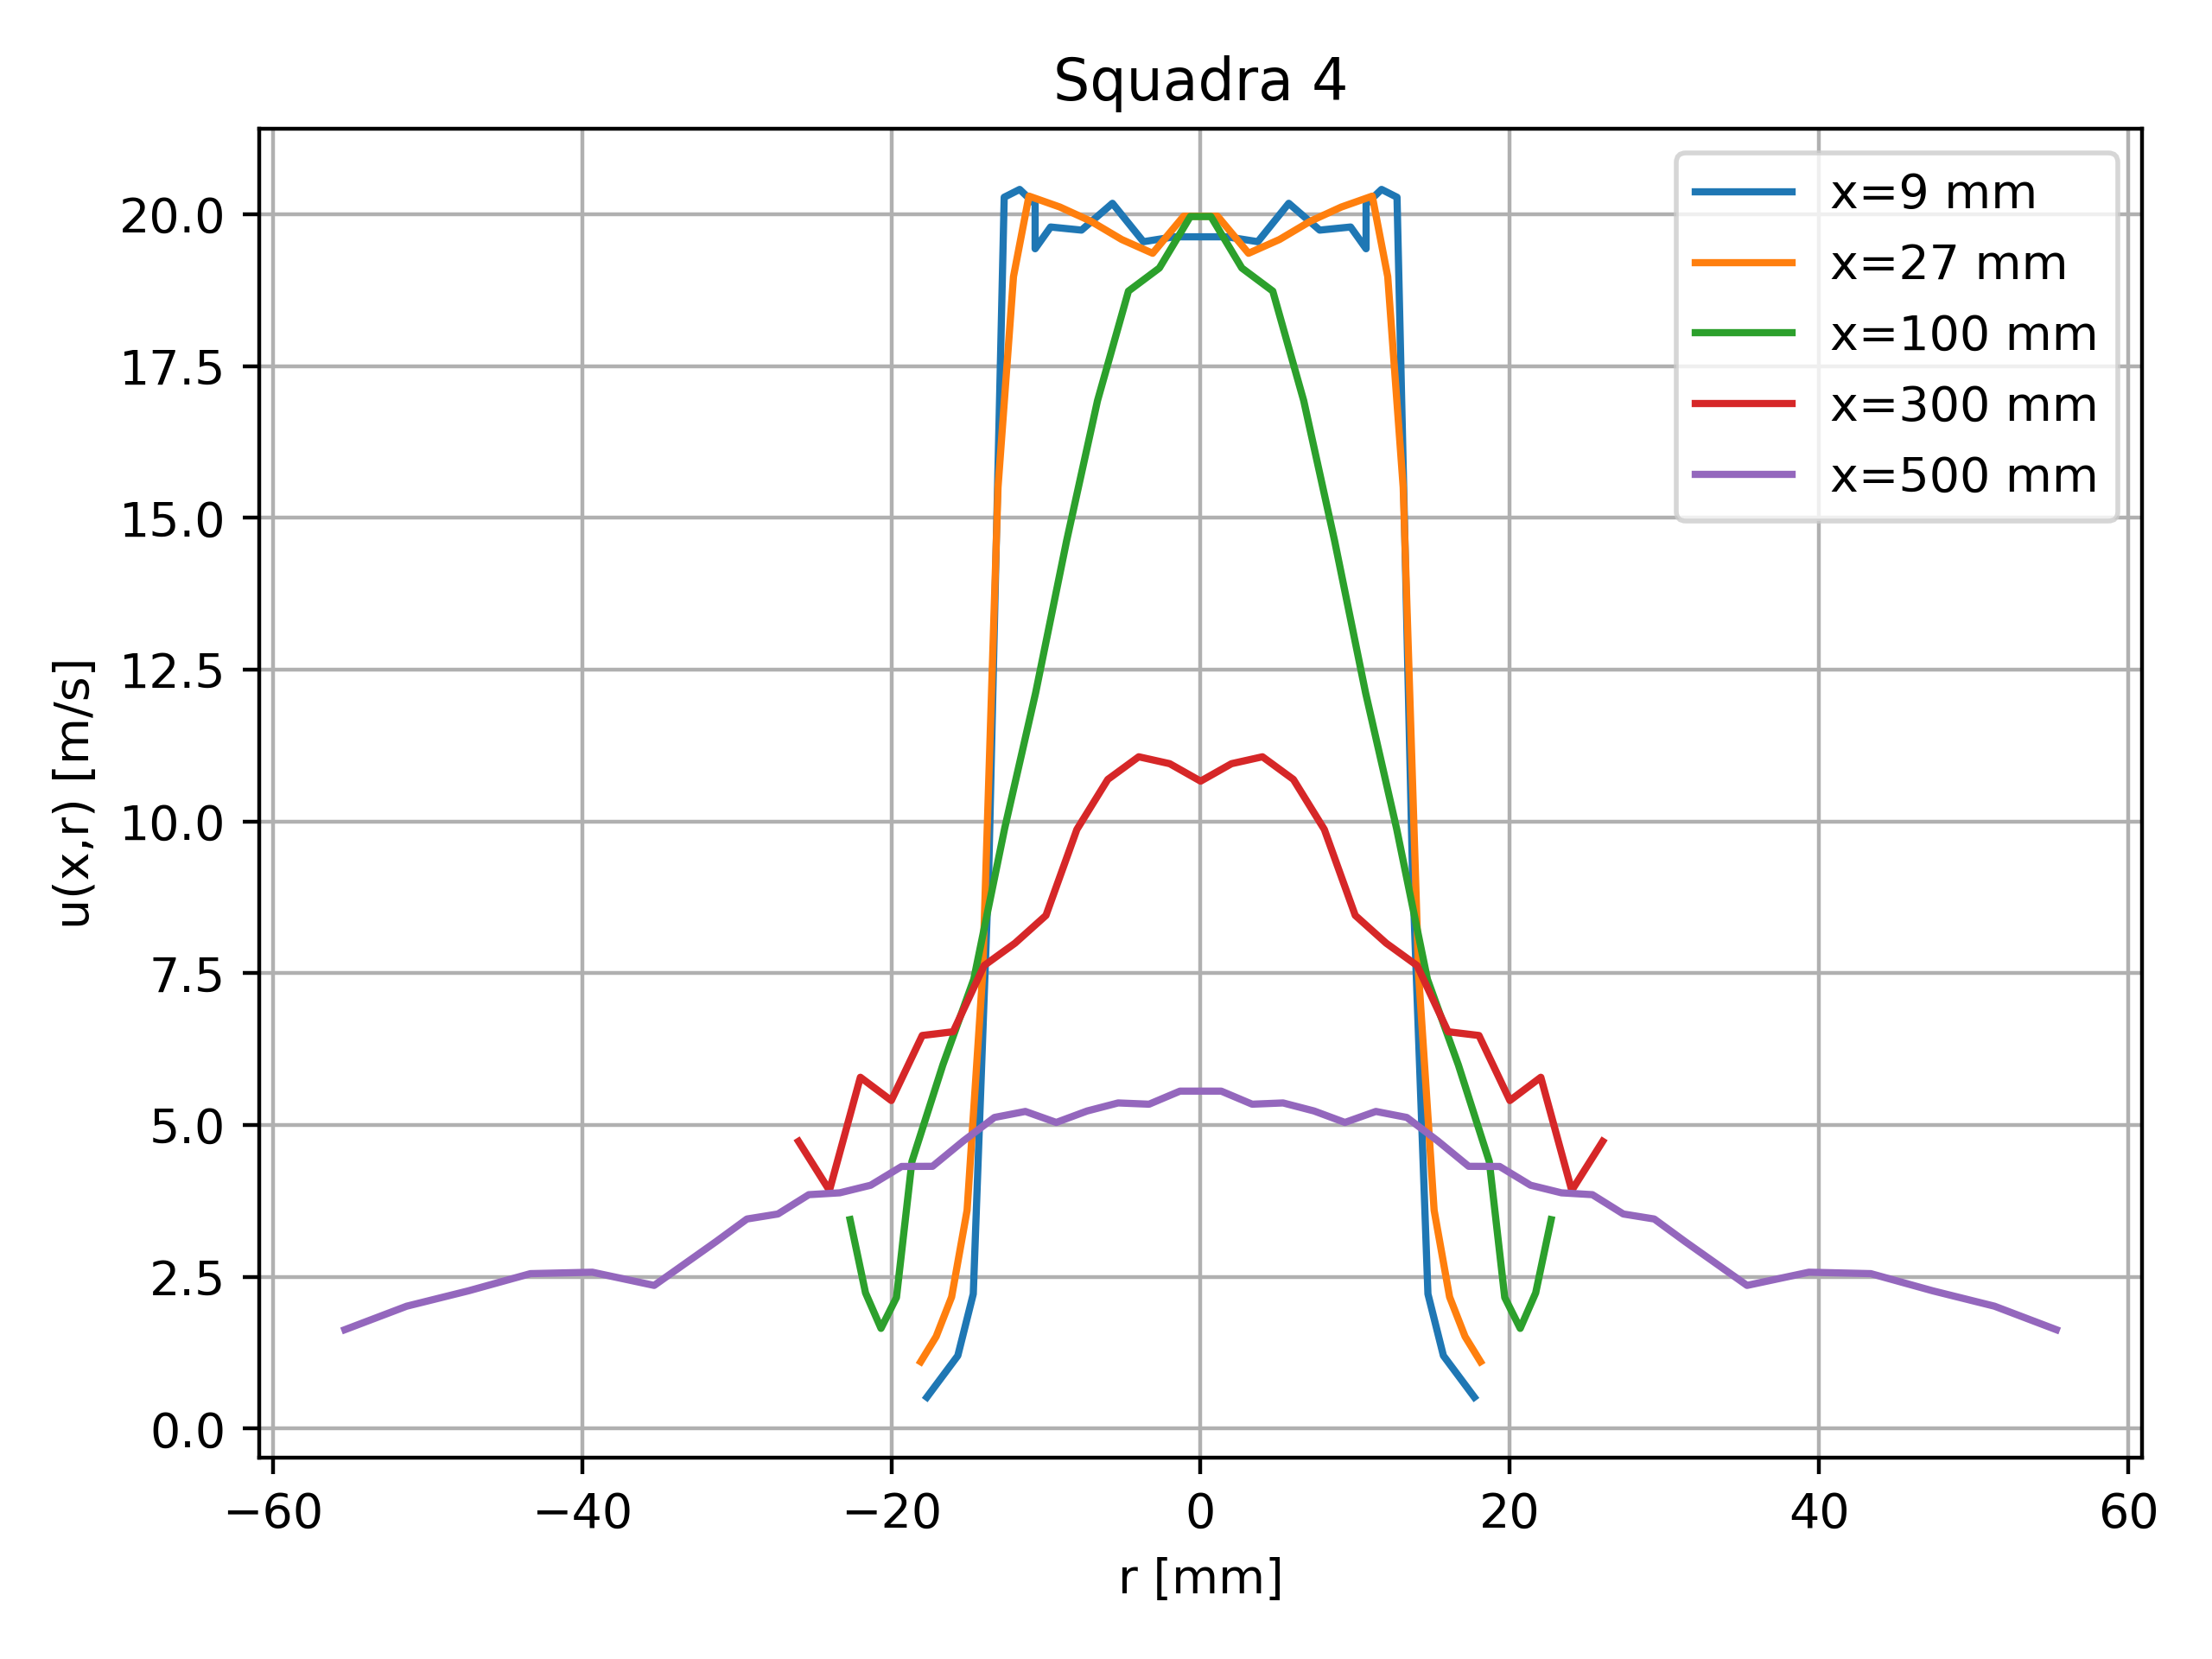
\includegraphics[width=.8\textwidth]{images/3/sq4.png}
    \caption{Profili di velocità per la quarta squadra}
\end{figure}

\noindent Per una migliore interpretazione, tali diagrammi possono essere visualizzati in uno spazio tridimensionale, così da esplicitare la distanza assiale $x$:
\begin{figure}[H]
    \centering
    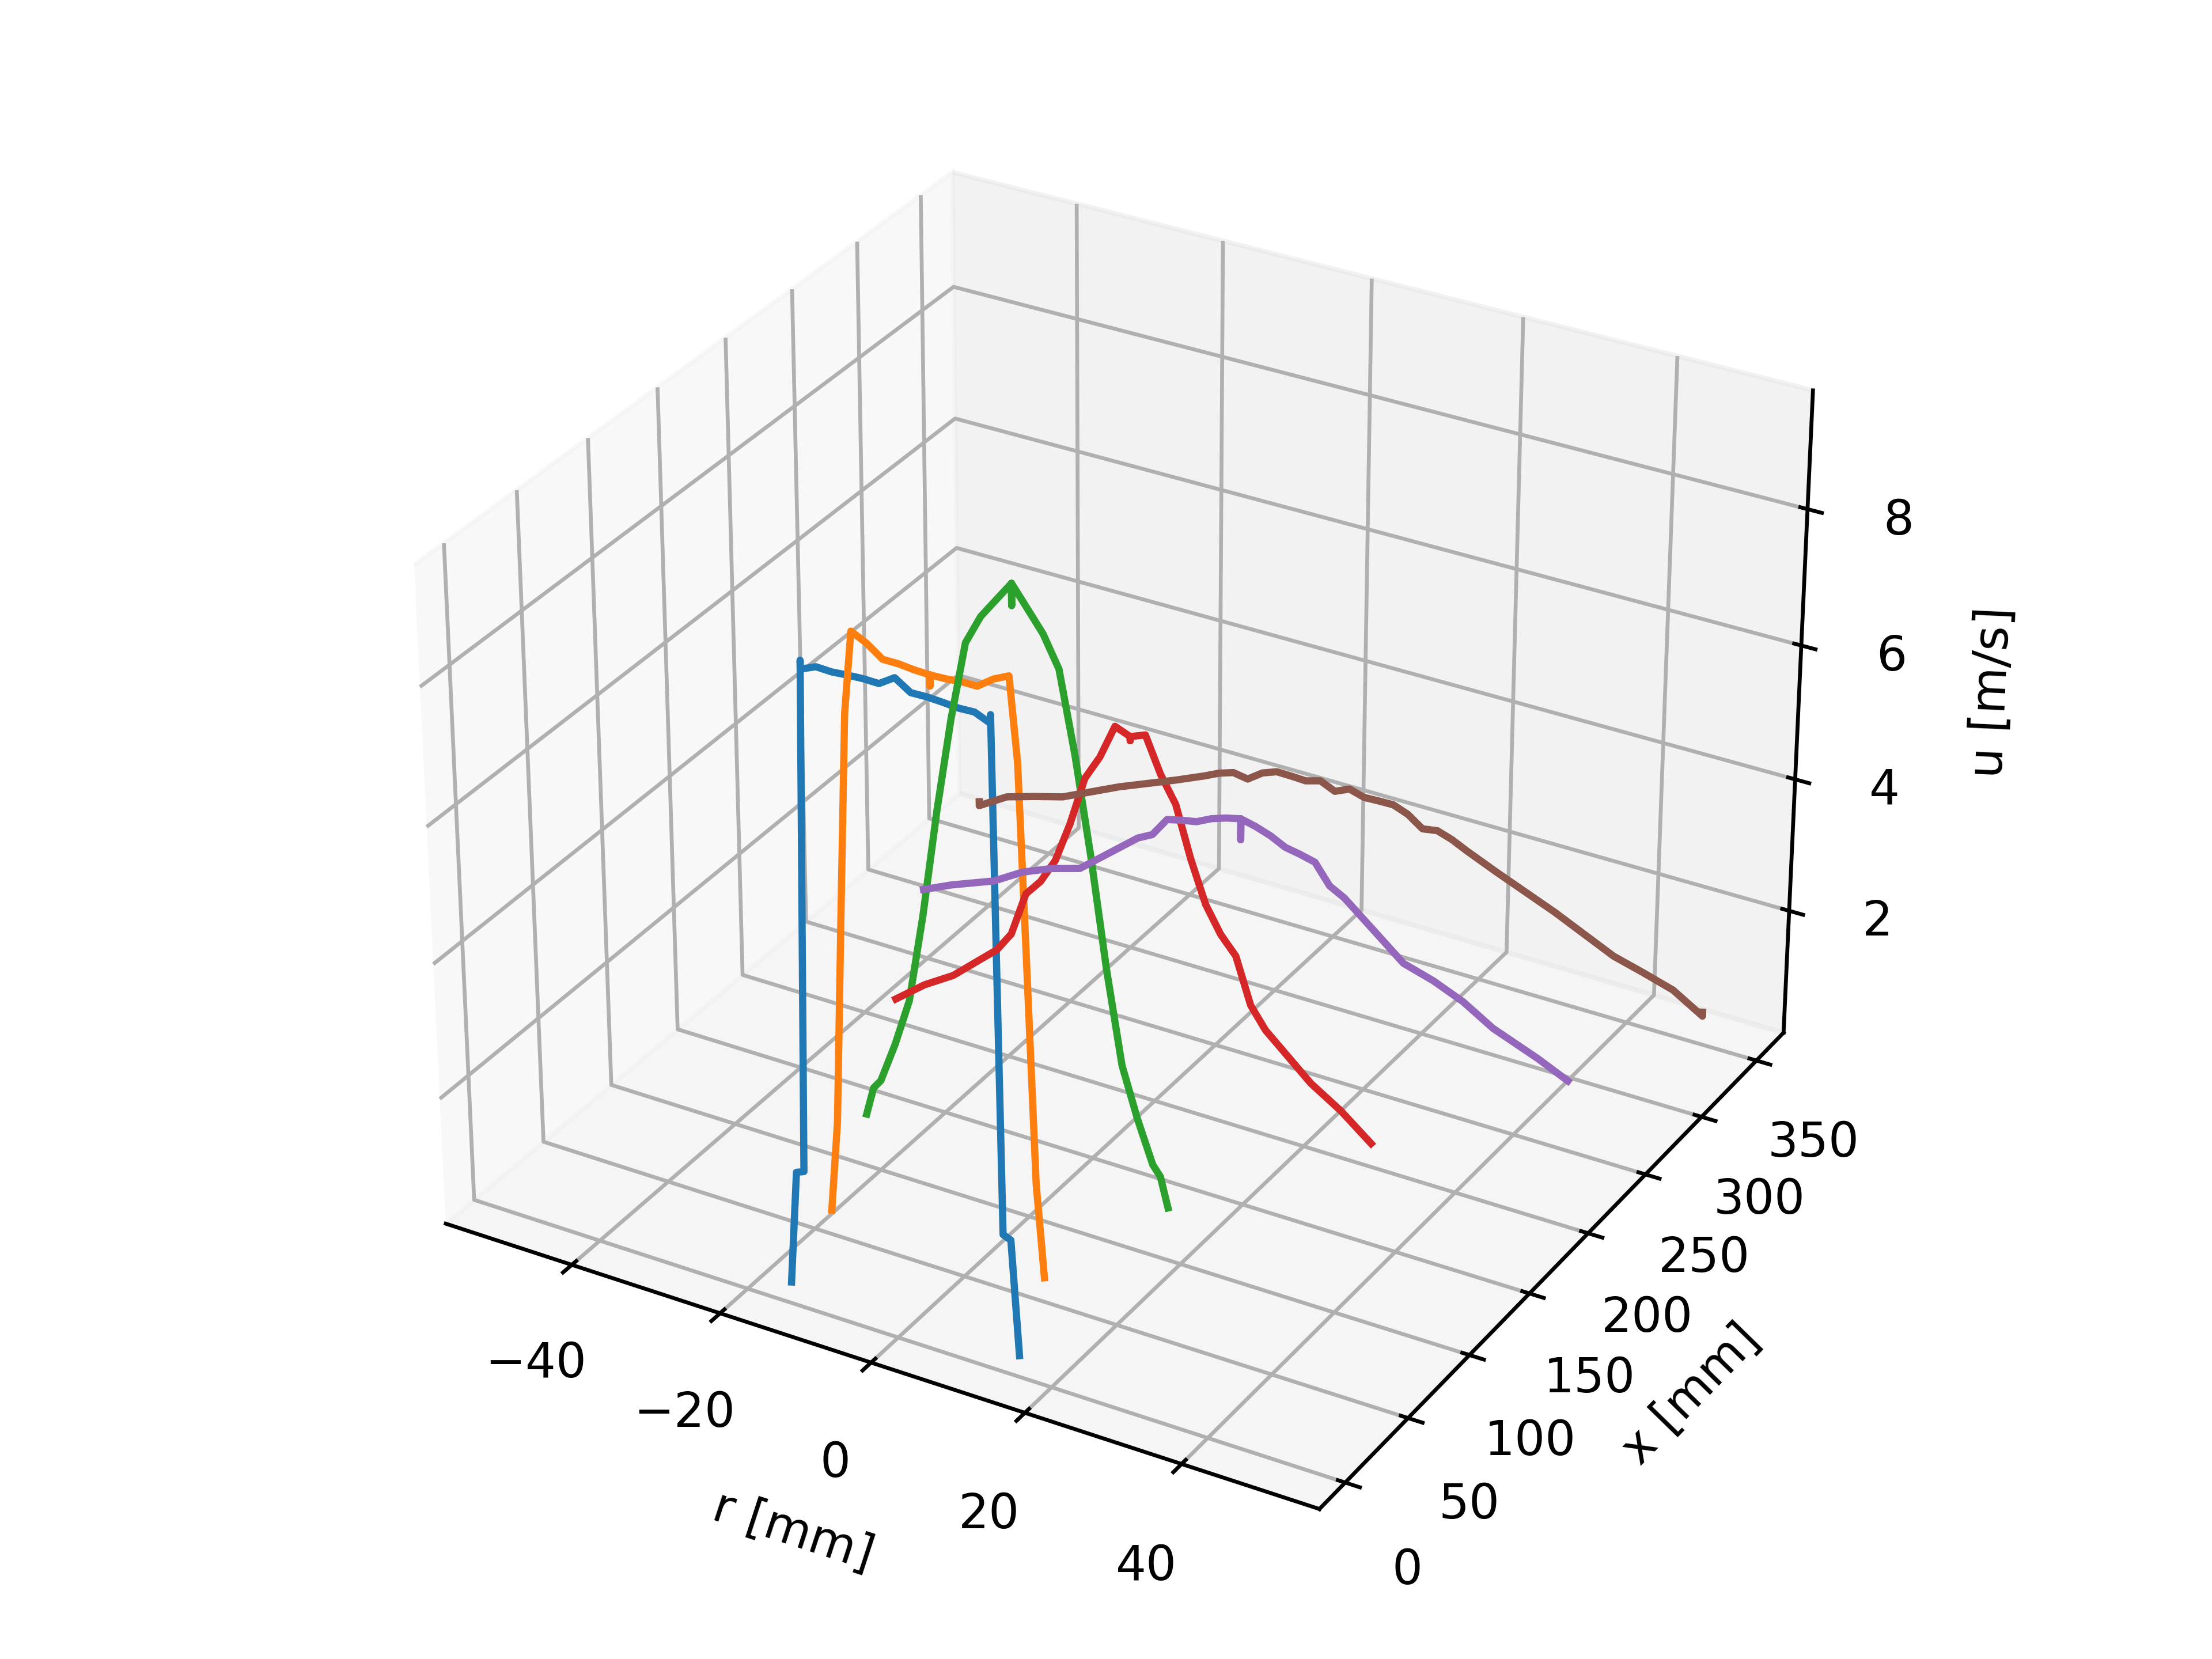
\includegraphics[width=.8\textwidth]{images/3/sq13d.png}
    \caption{Profili di velocità per la prima squadra}
\end{figure}
\begin{figure}[H]
    \centering
    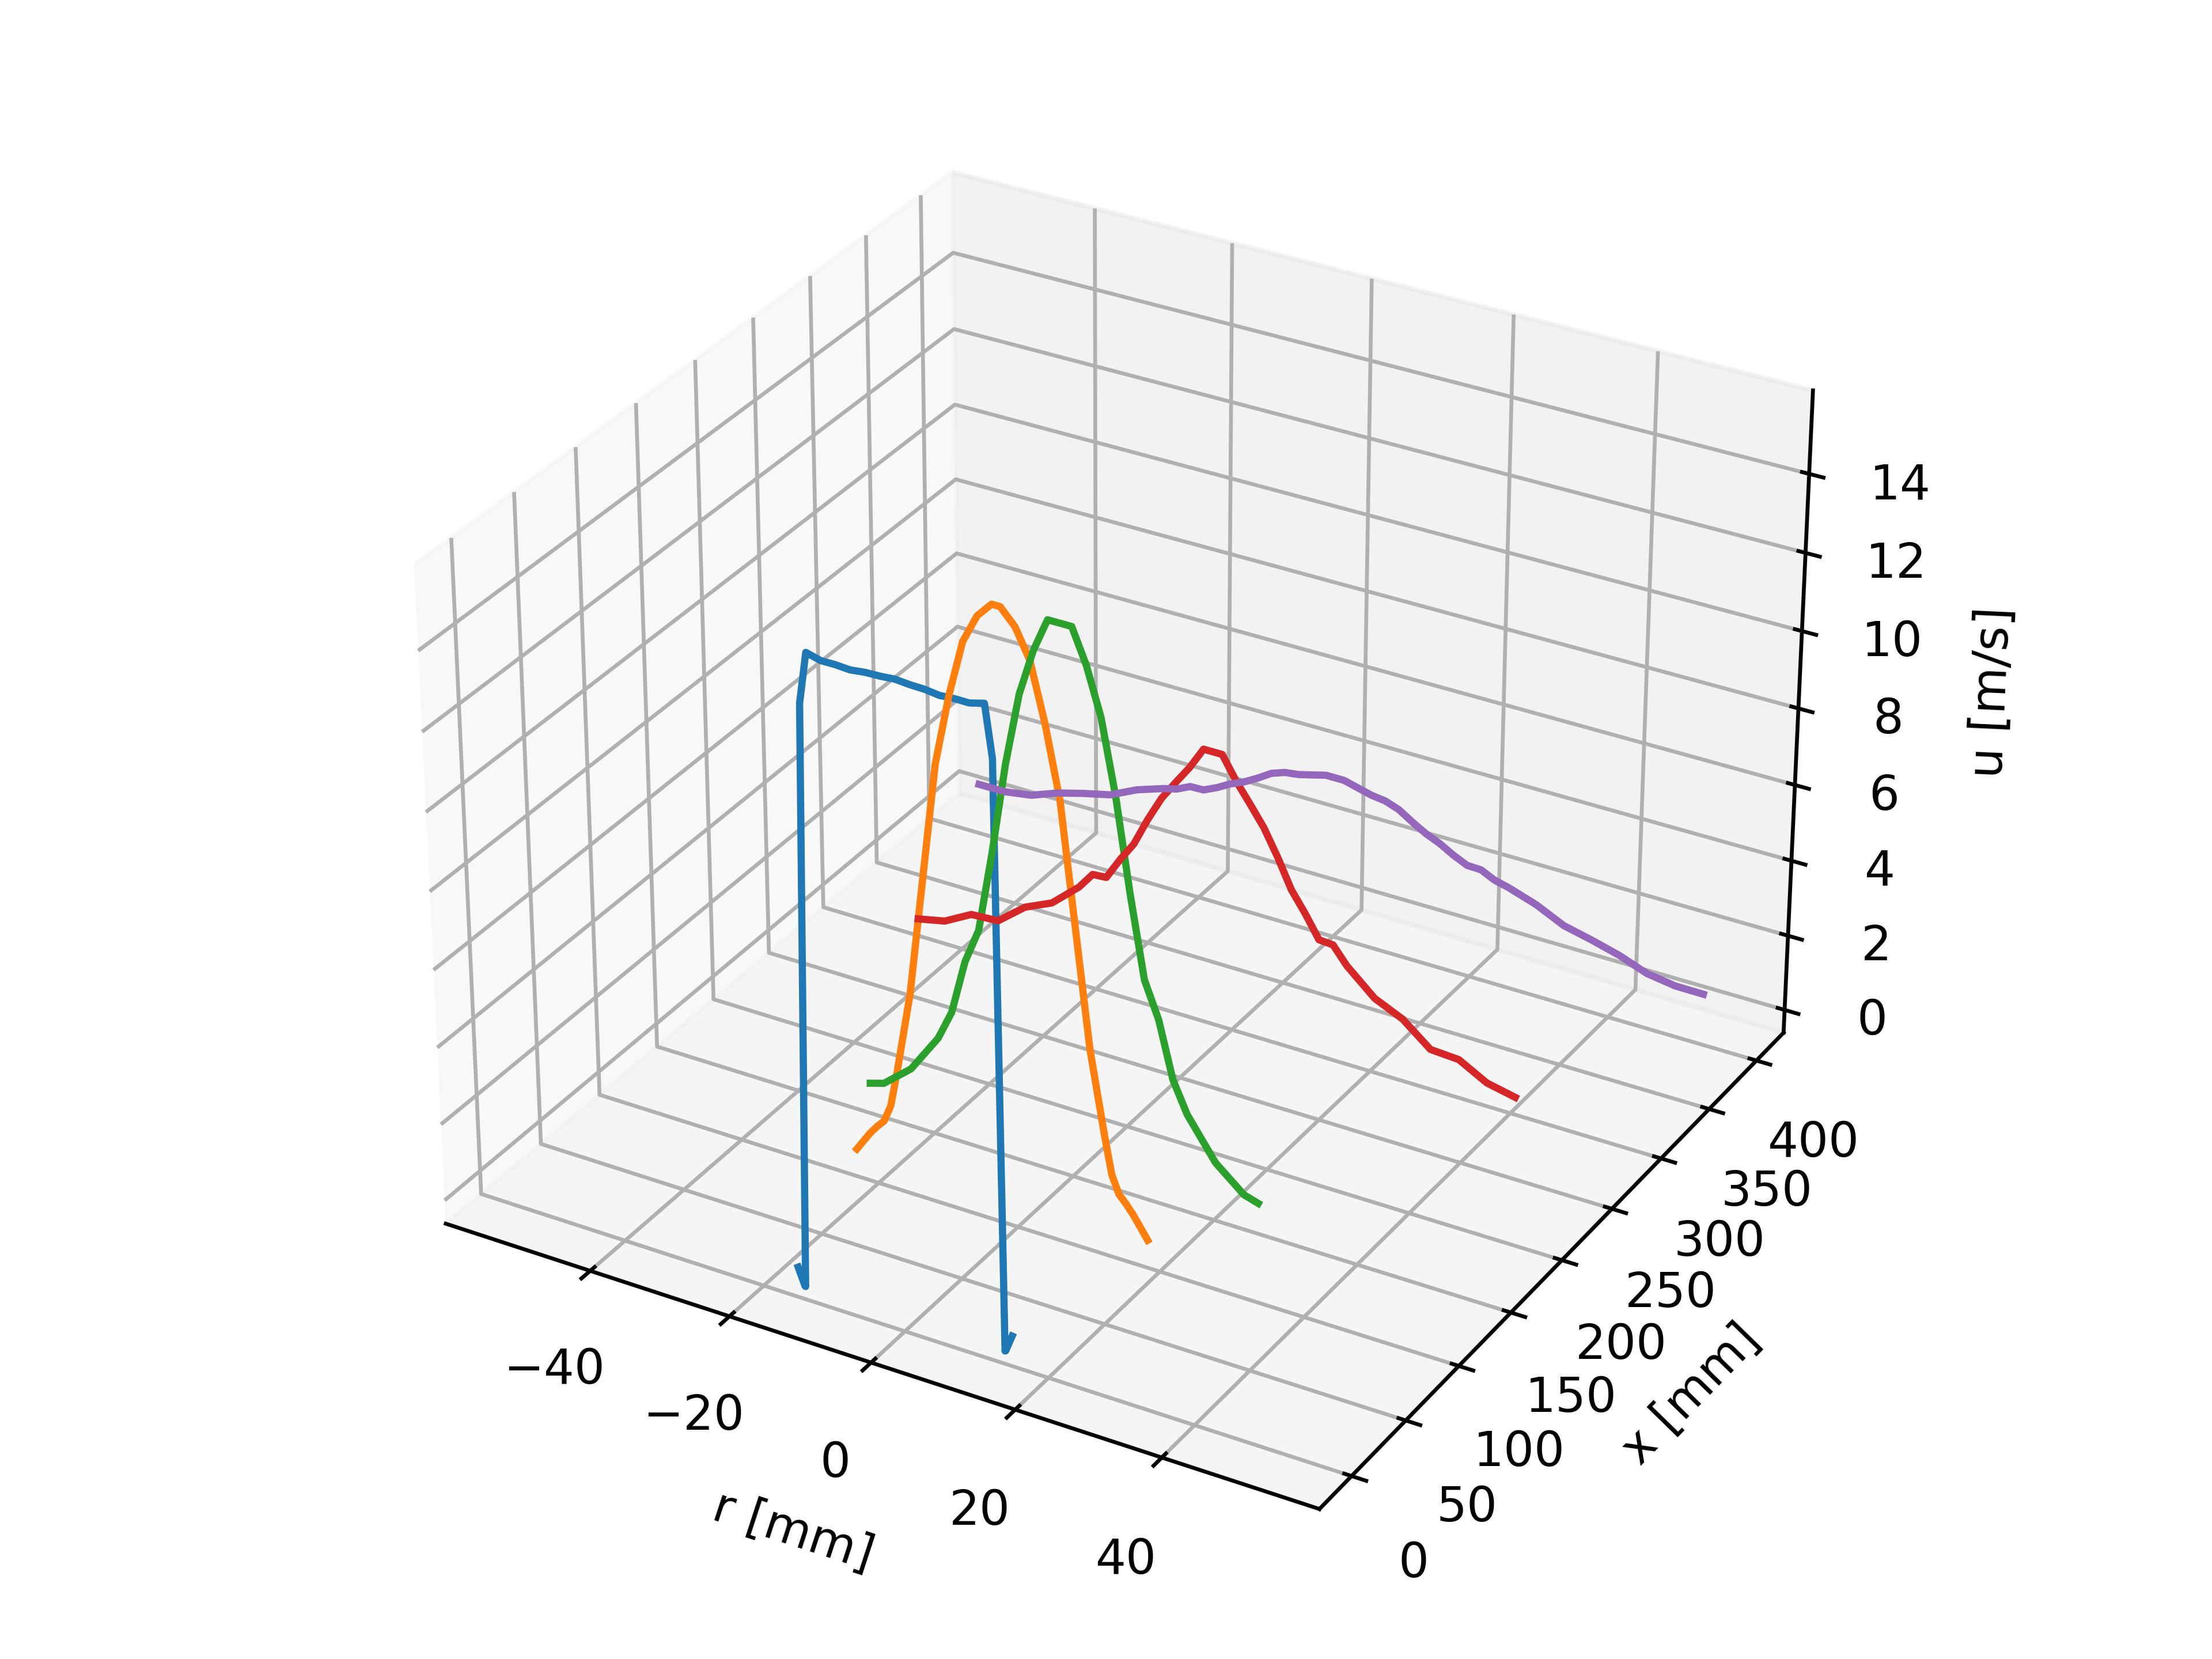
\includegraphics[width=.92\textwidth]{images/3/sq23d.png}
    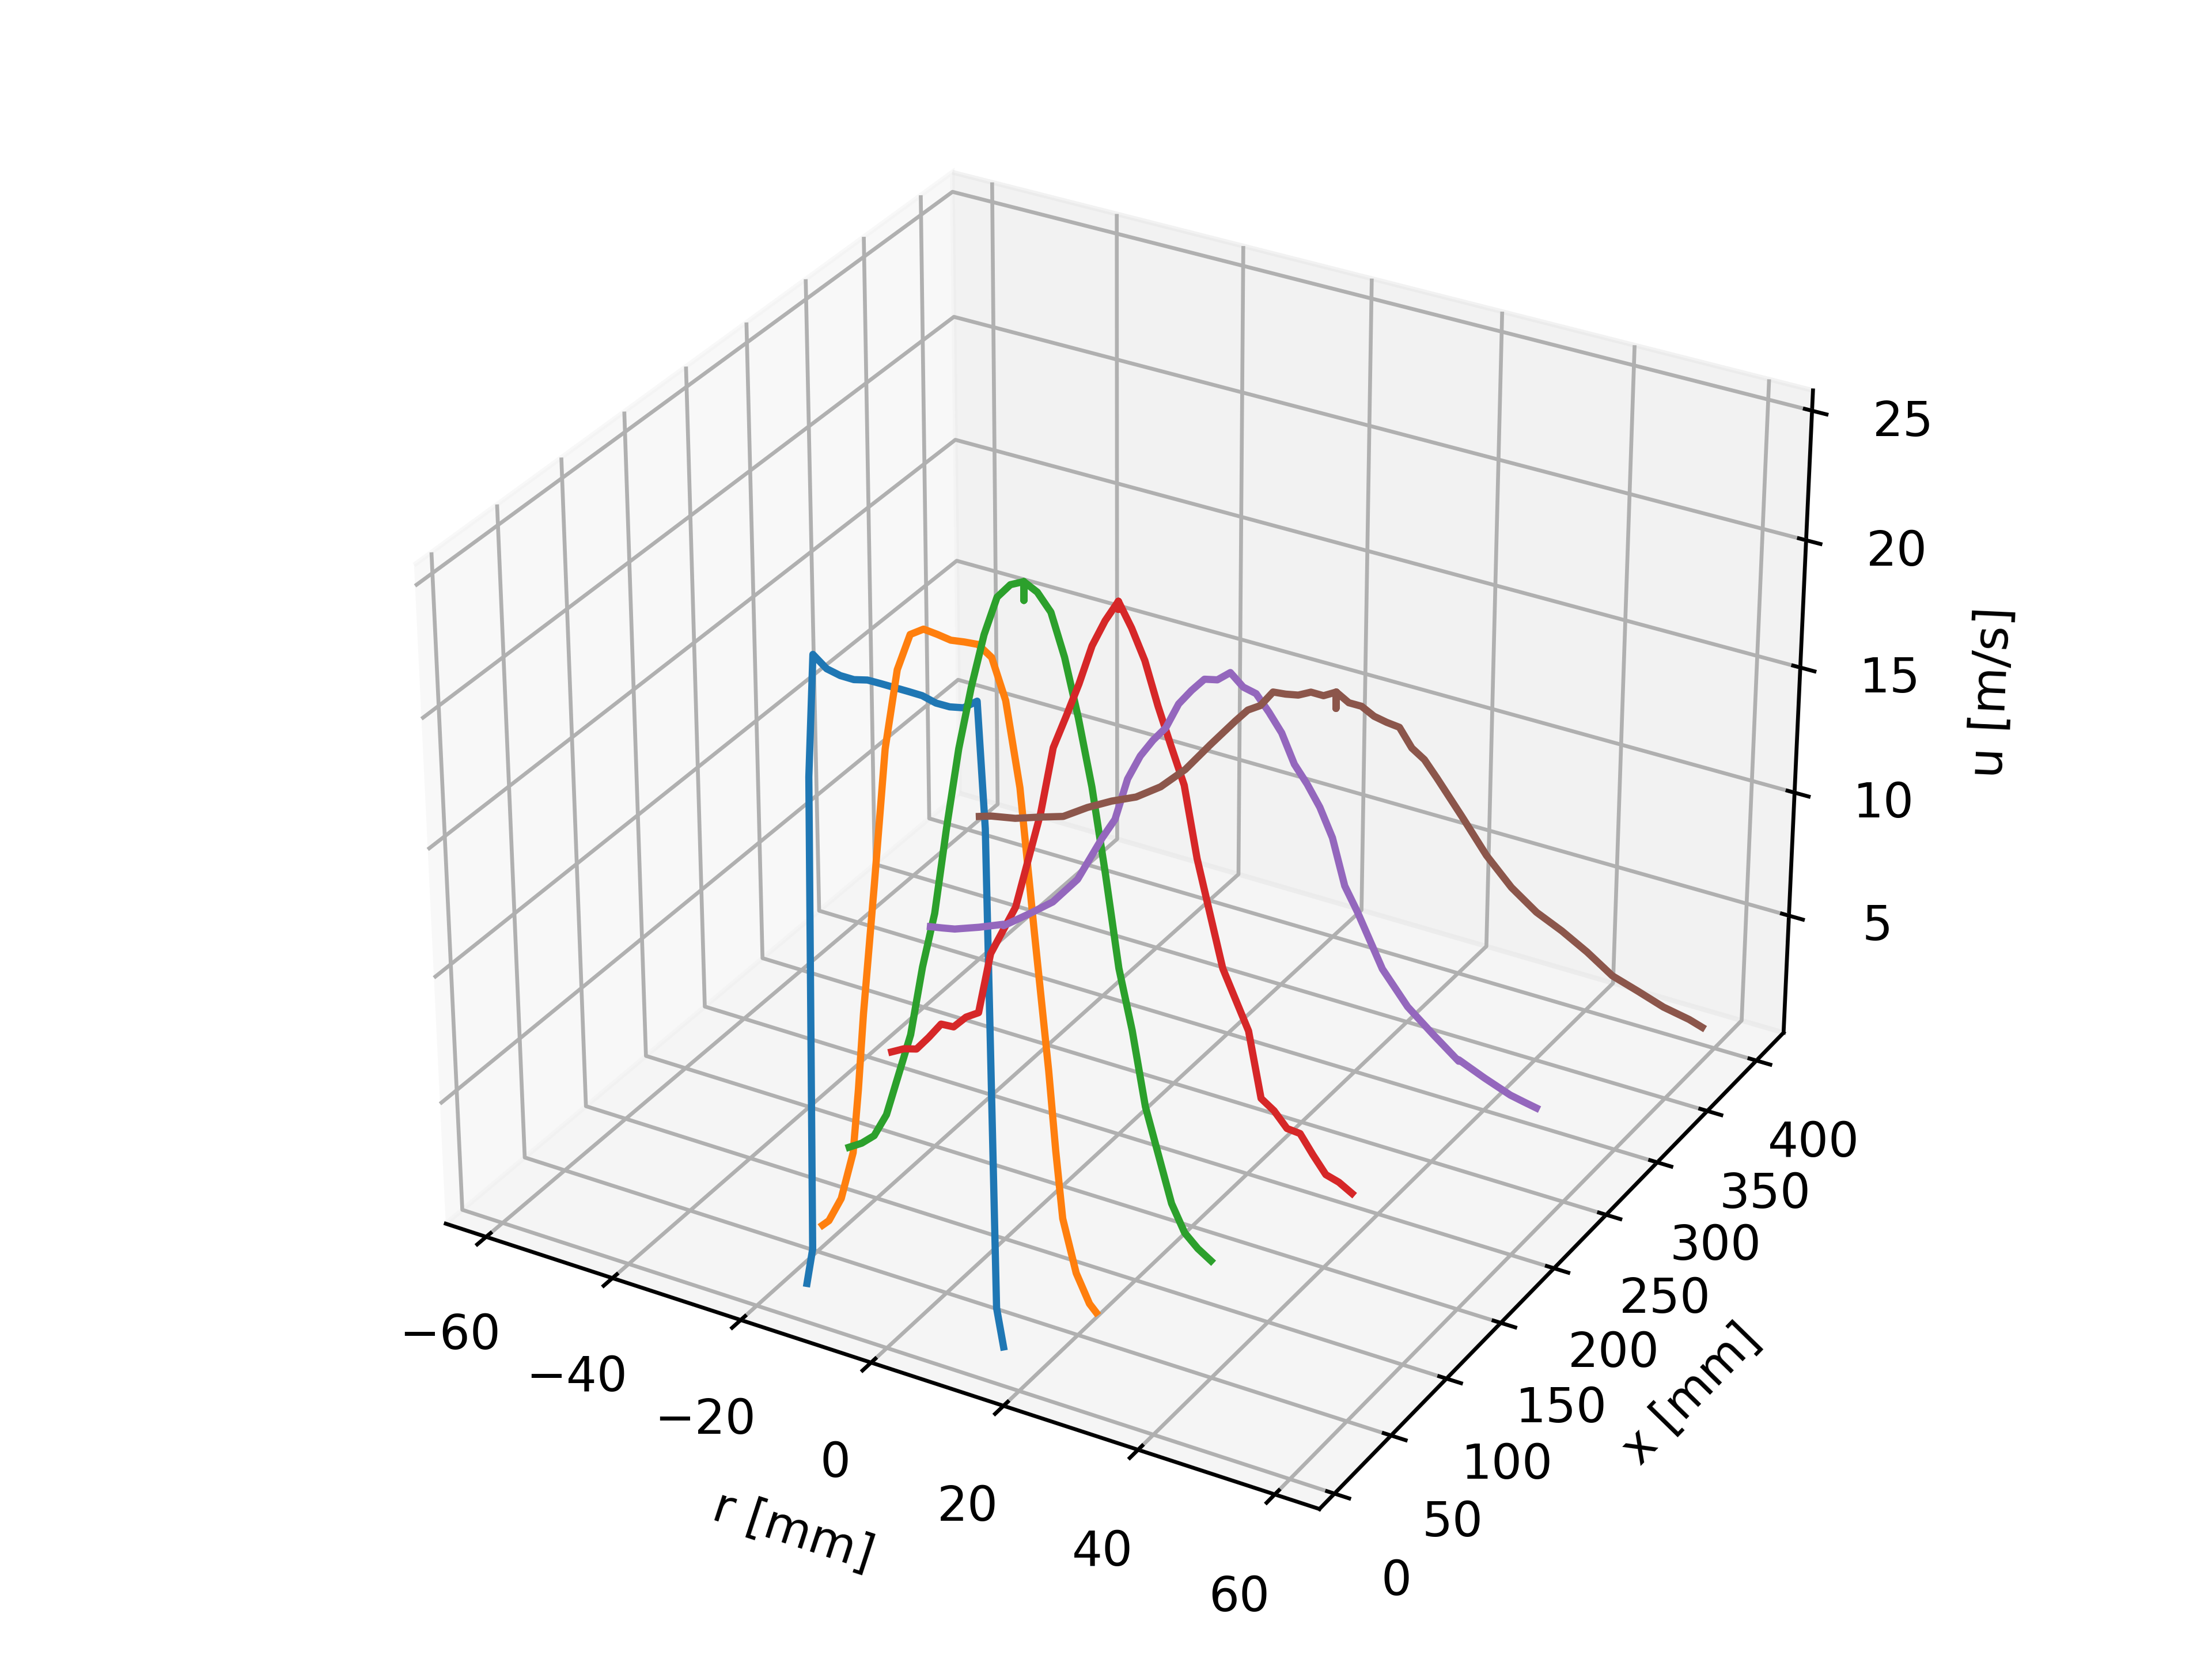
\includegraphics[width=.92\textwidth]{images/3/sq33d.png}
    \caption{Profili di velocità per la seconda e per la terza squadra}
\end{figure}
\begin{figure}[H]
    \centering
    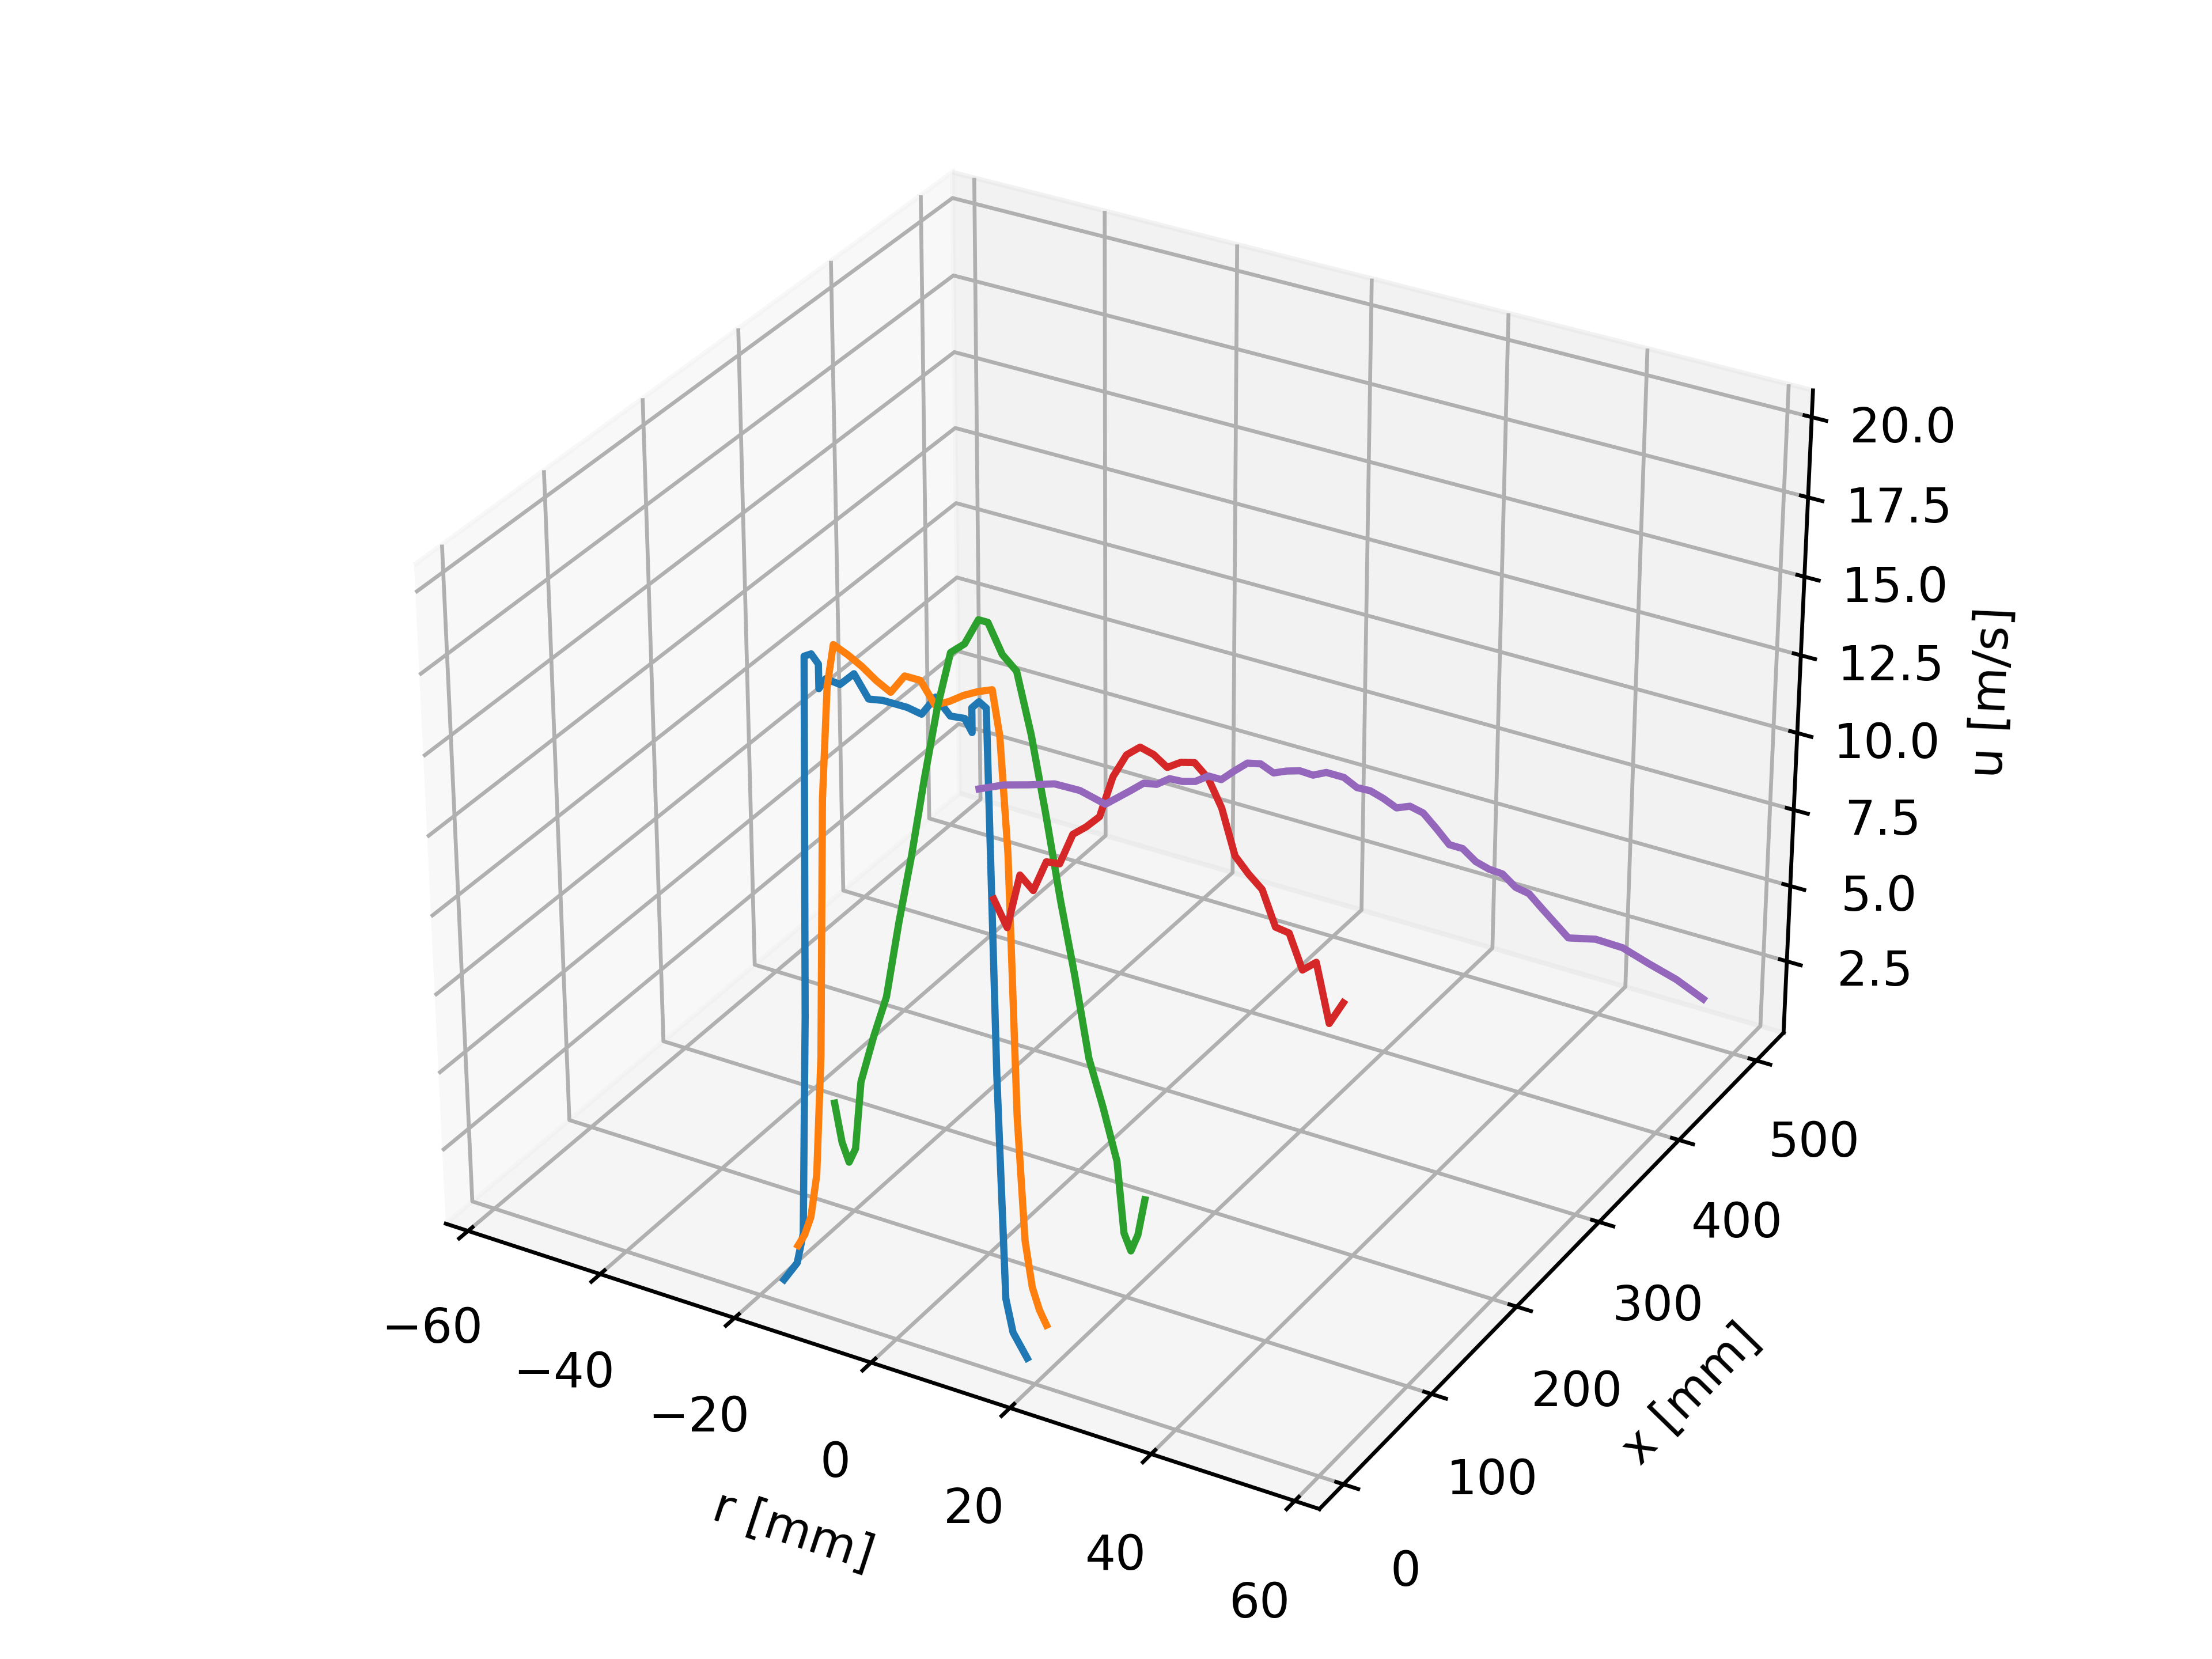
\includegraphics[width=.85\textwidth]{images/3/sq43d.png}
    \caption{Profili di velocità per la quarta squadra}
\end{figure}

\noindent Si evidenziano degli effetti spuri in prossimità dell'asse del getto, in particolar modo nel getto relativo alla quarta squadra. Questi possono essere dovuti a vari fattori, come ad esempio un non perfetto allineamento della slitta assiale con l'asse del getto. Tali effetti sono mitigati come indicato nel codice Python in appendice \ref{b3}.\\\\
Si nota come in prossimità dell'orifizio i profili di velocità presentano un tratto rettilineo. Tale caratteristica mette in mostra il cuore potenziale del getto, in cui la velocità è costante. Pertanto, si può ricavare la velocità iniziale del getto:
\begin{equation*}
    U_0 = U(r=0, x=0)
\end{equation*}
Utilizzando tale velocità si calcola il numero di Reynolds per i quattro flussi in esame:
\begin{equation*}
    Re = \frac{\rho U_0 D_j}{\mu}
\end{equation*}
Questi corrispondono a 15905, 26321, 42207 e 34102.\\\\
I profili di velocità che presentano una porzione del cuore potenziale del getto caratterizzano la mixing region del getto, mentre i profili successivi caratterizzano la zona di transizione e la zona self-similar.
\newpage
\noindent Si possono ora diagrammare i profili di velocità adimensionali, ad esempio normalizzando la velocità con la velocità iniziale del getto e la distanza radiale con il diametro del getto:
\begin{equation*}
    \frac U {U_0} = f\left(\frac r{D_j} \right)
\end{equation*}
\begin{figure}[H]
    \centering
    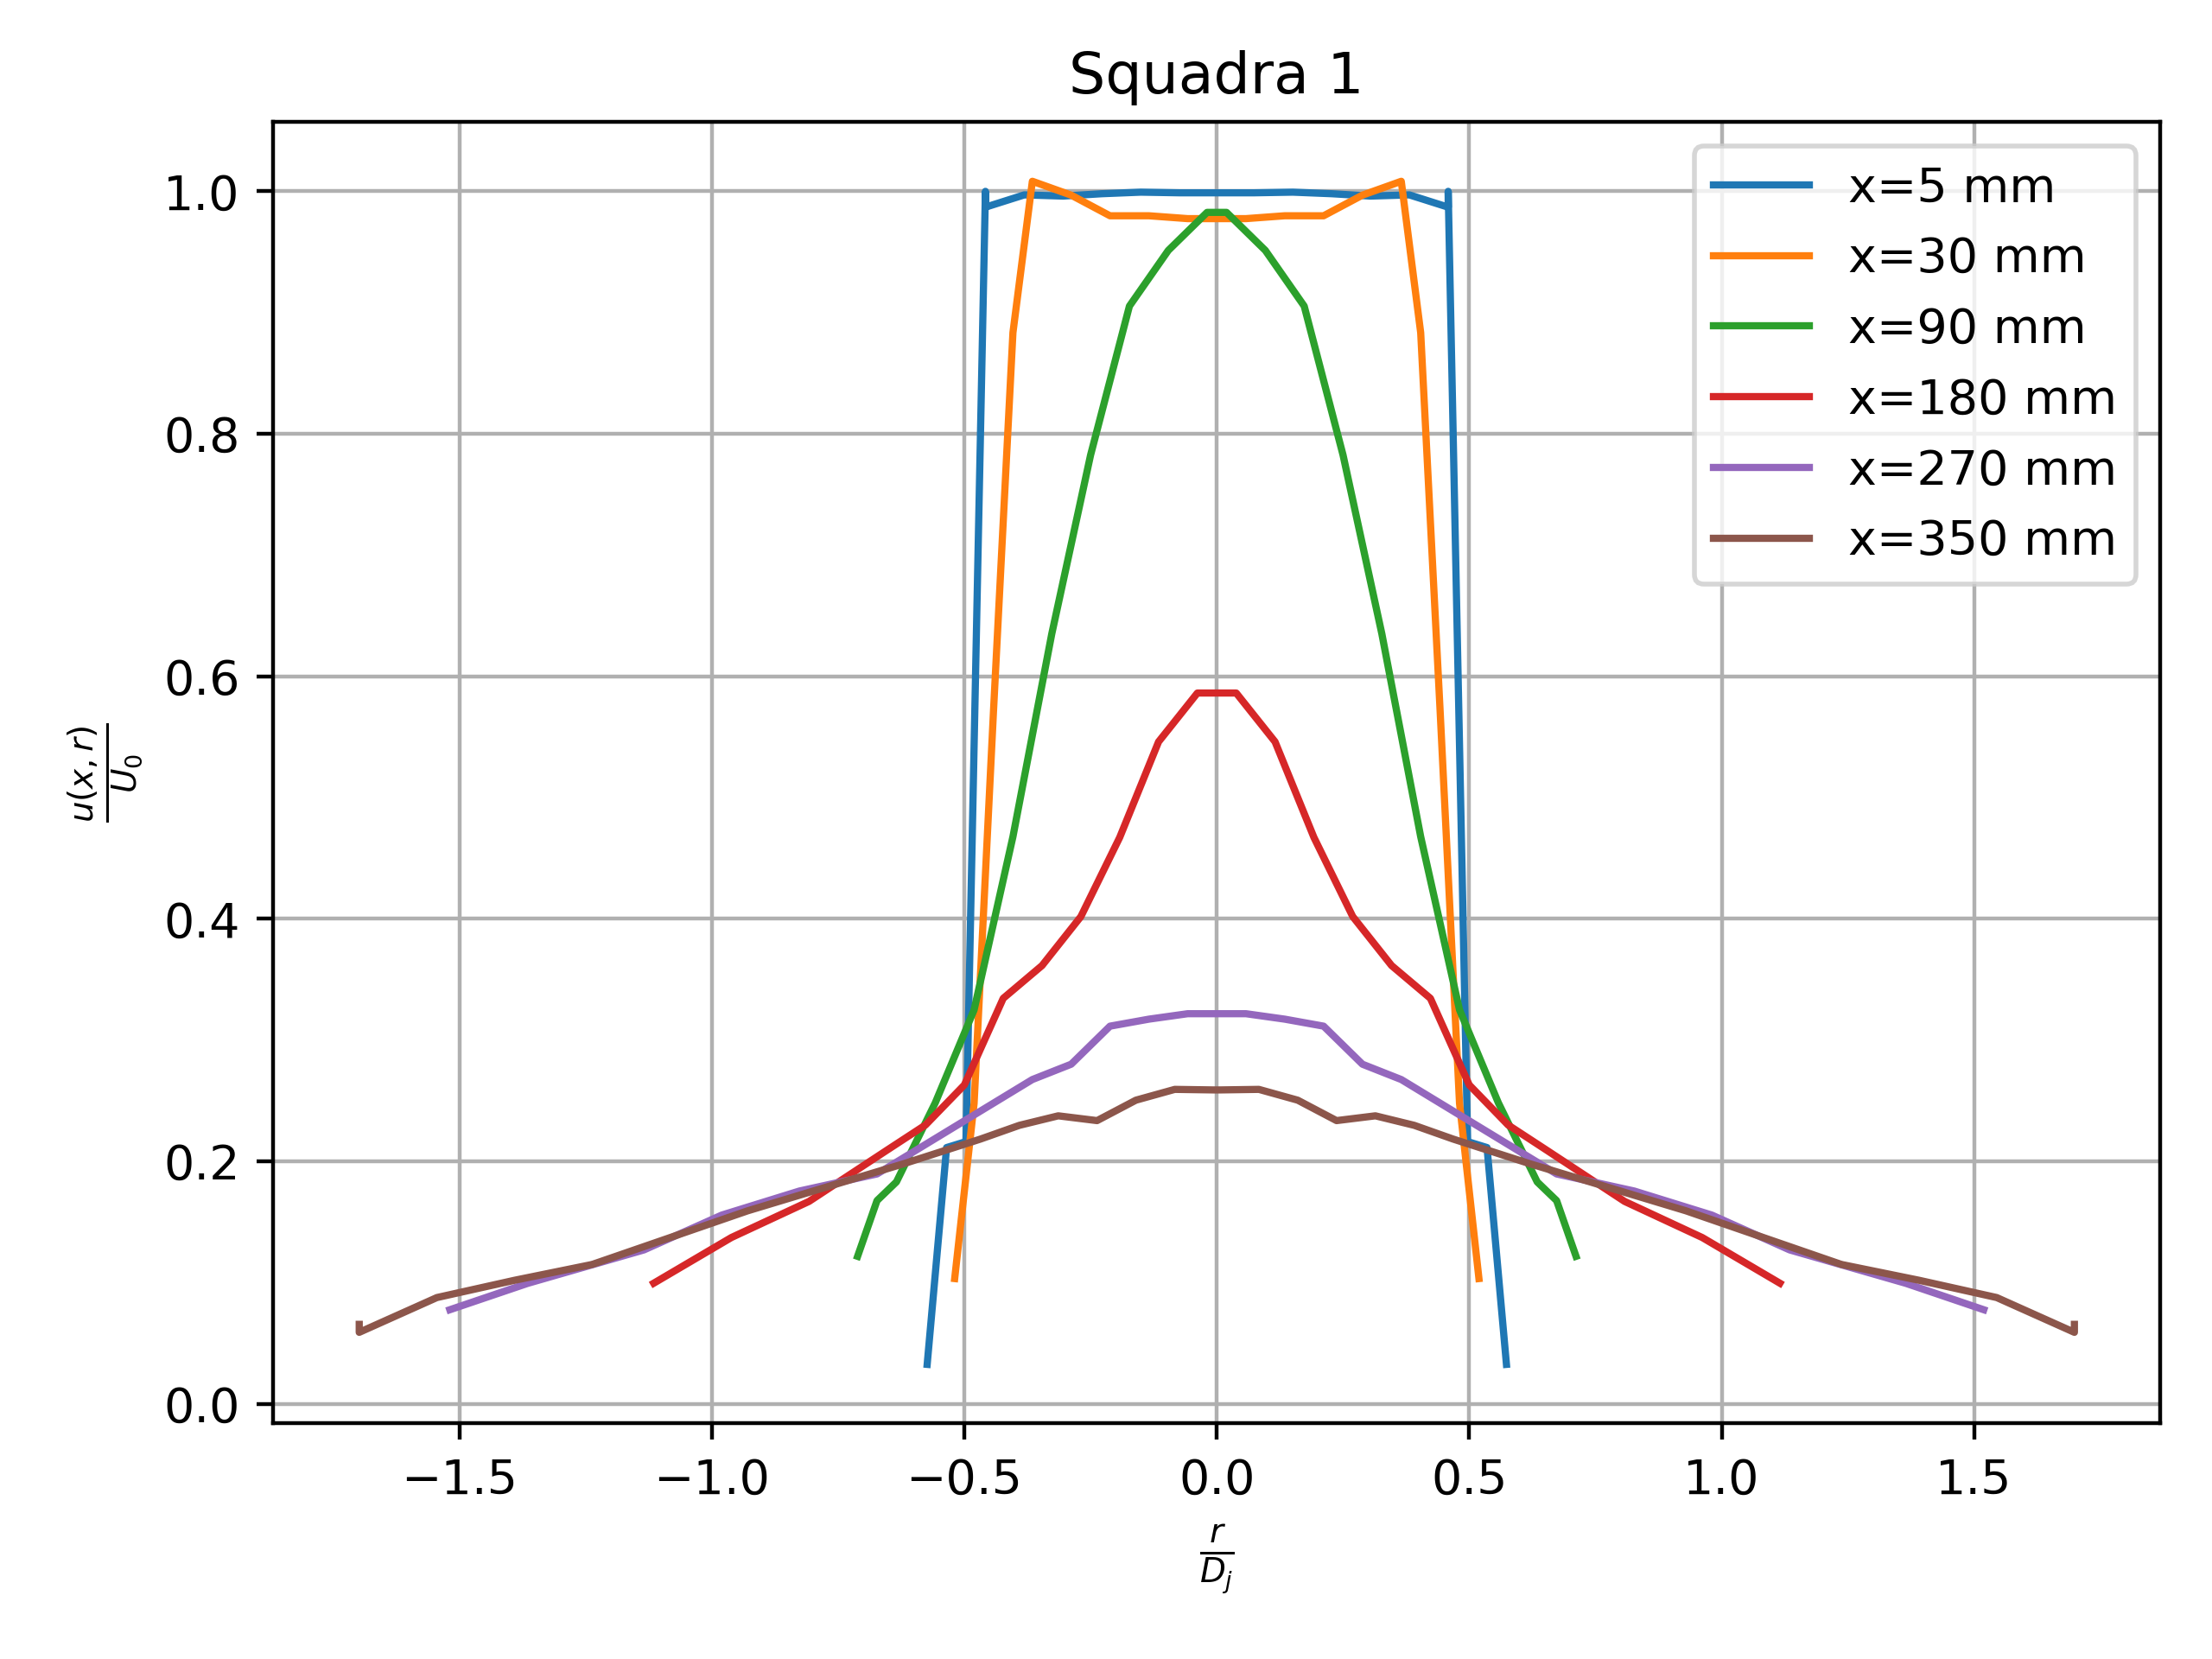
\includegraphics[width=.77\textwidth]{images/3/sq1u0.png}
    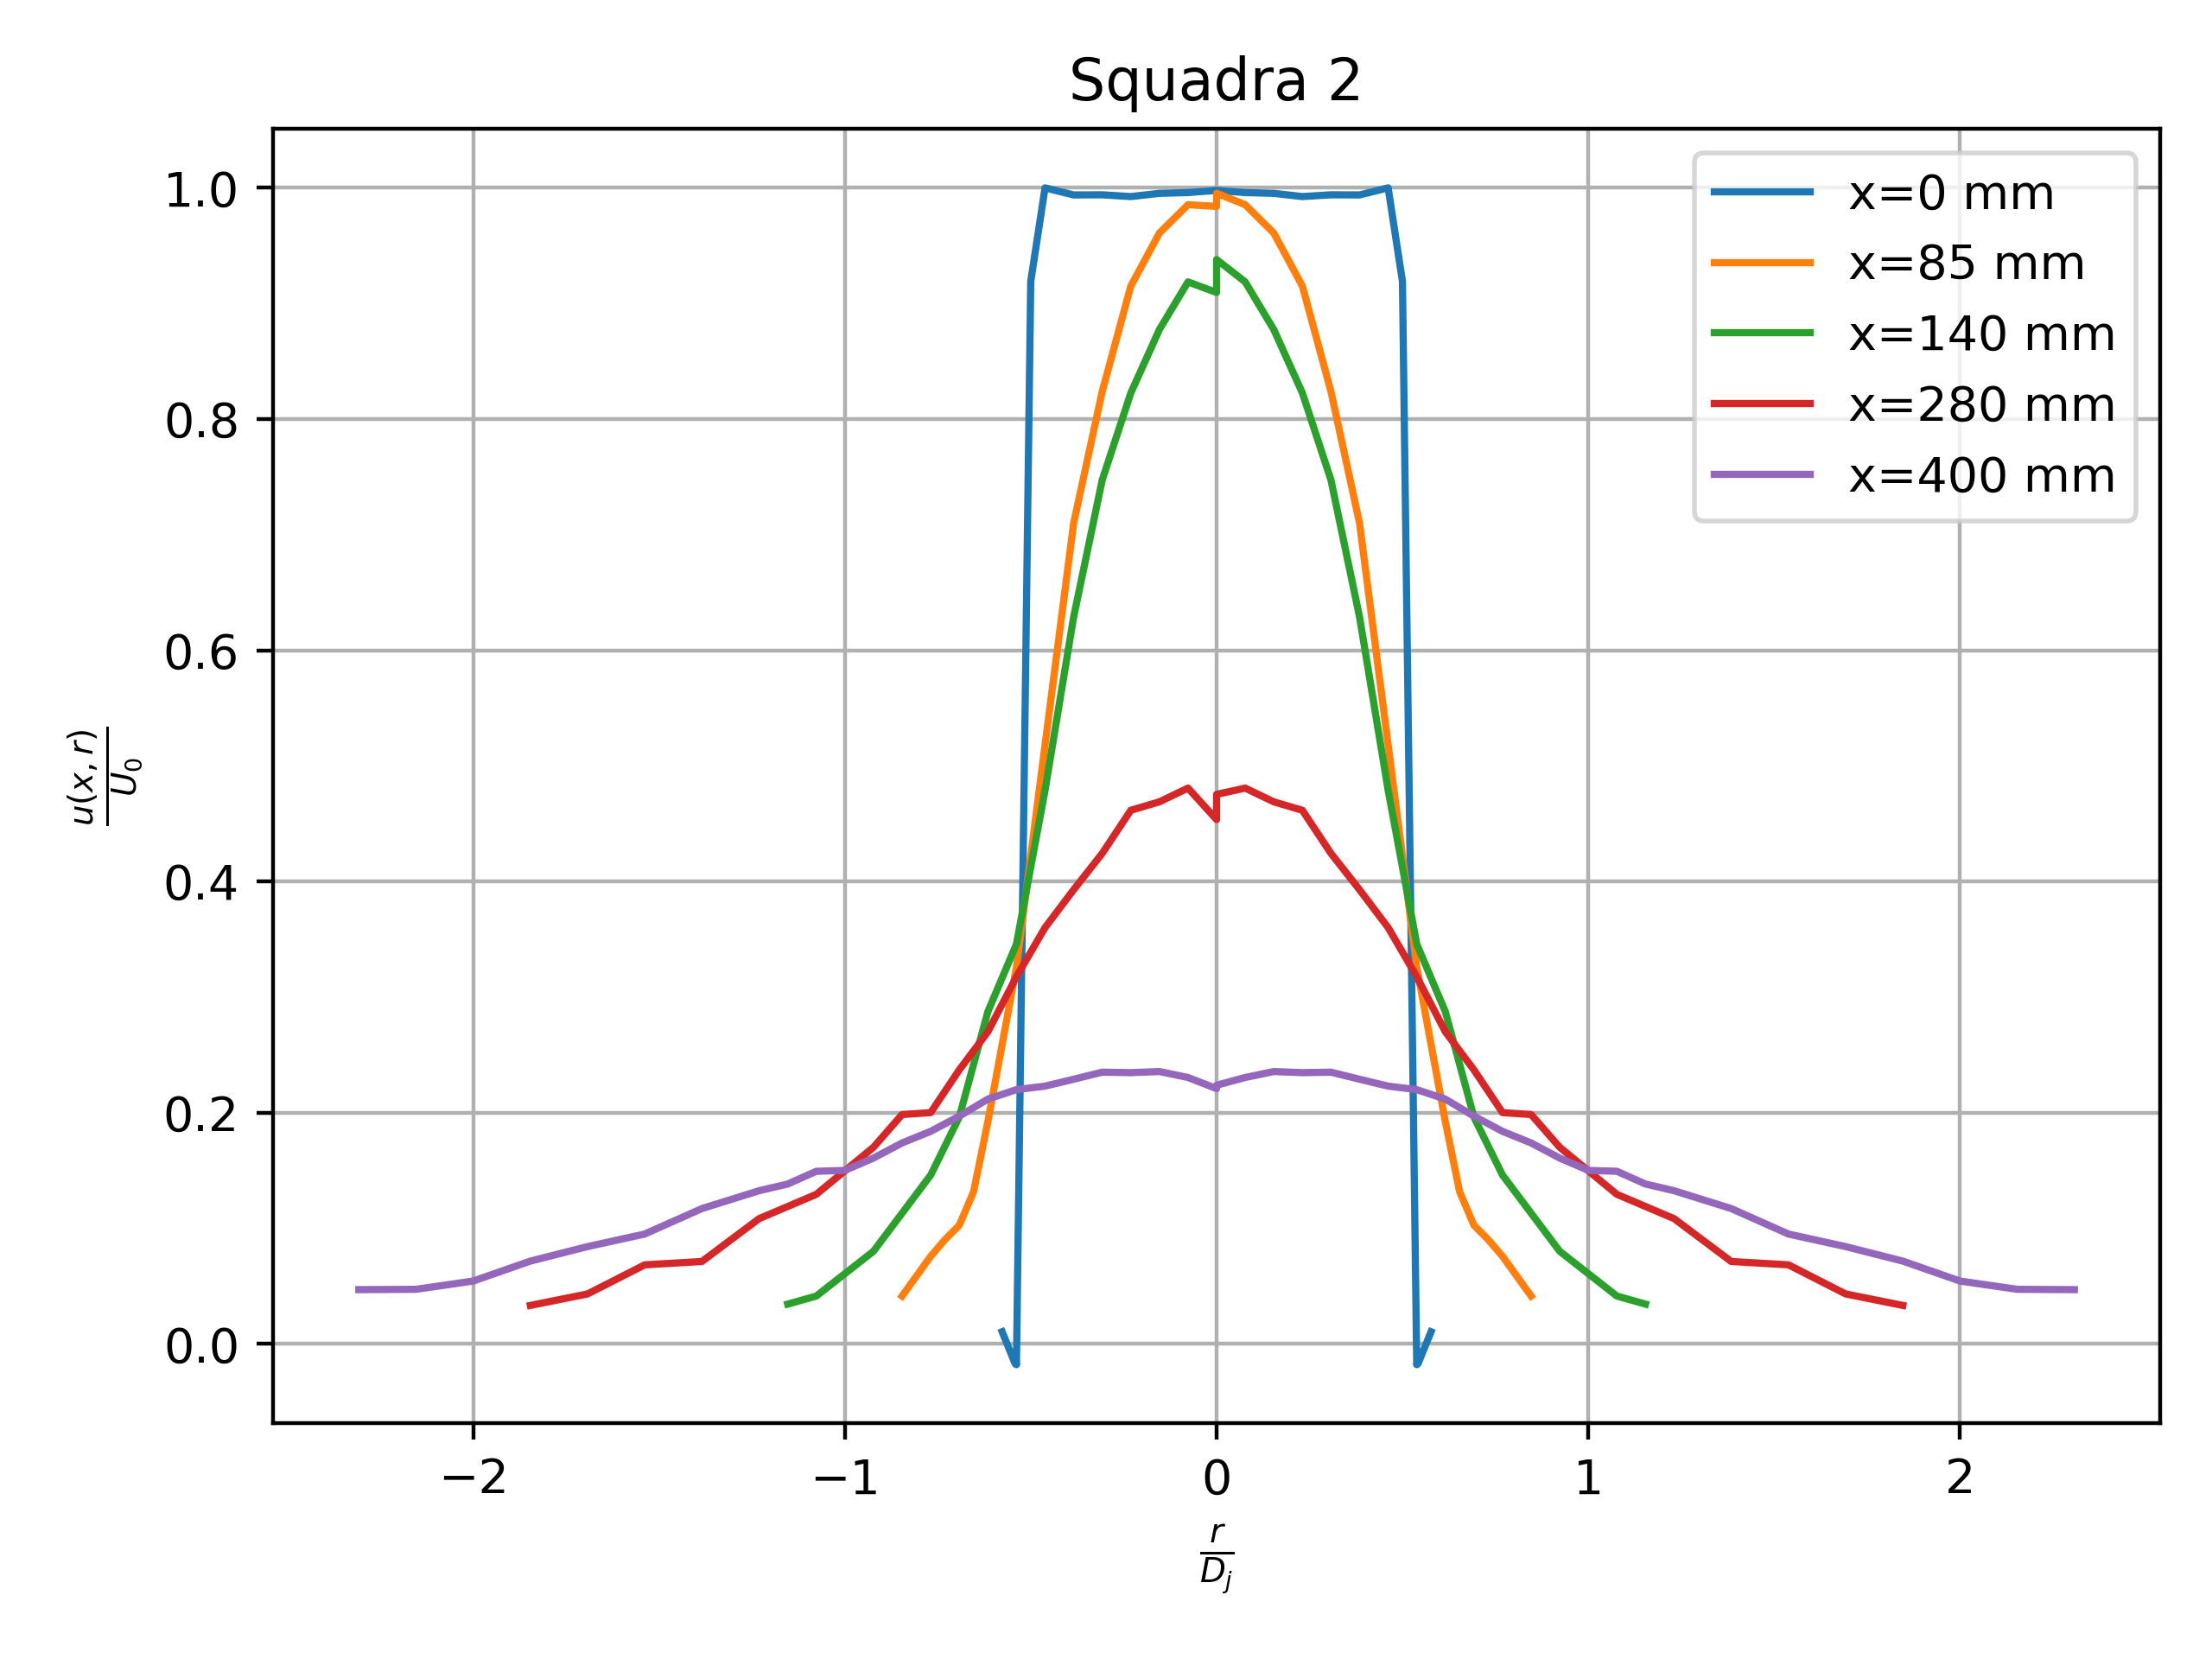
\includegraphics[width=.77\textwidth]{images/3/sq2u0.png}
    \caption{Profili di velocità adimensionali per la prima e per la seconda squadra}
\end{figure}
\begin{figure}[ht]
    \centering
    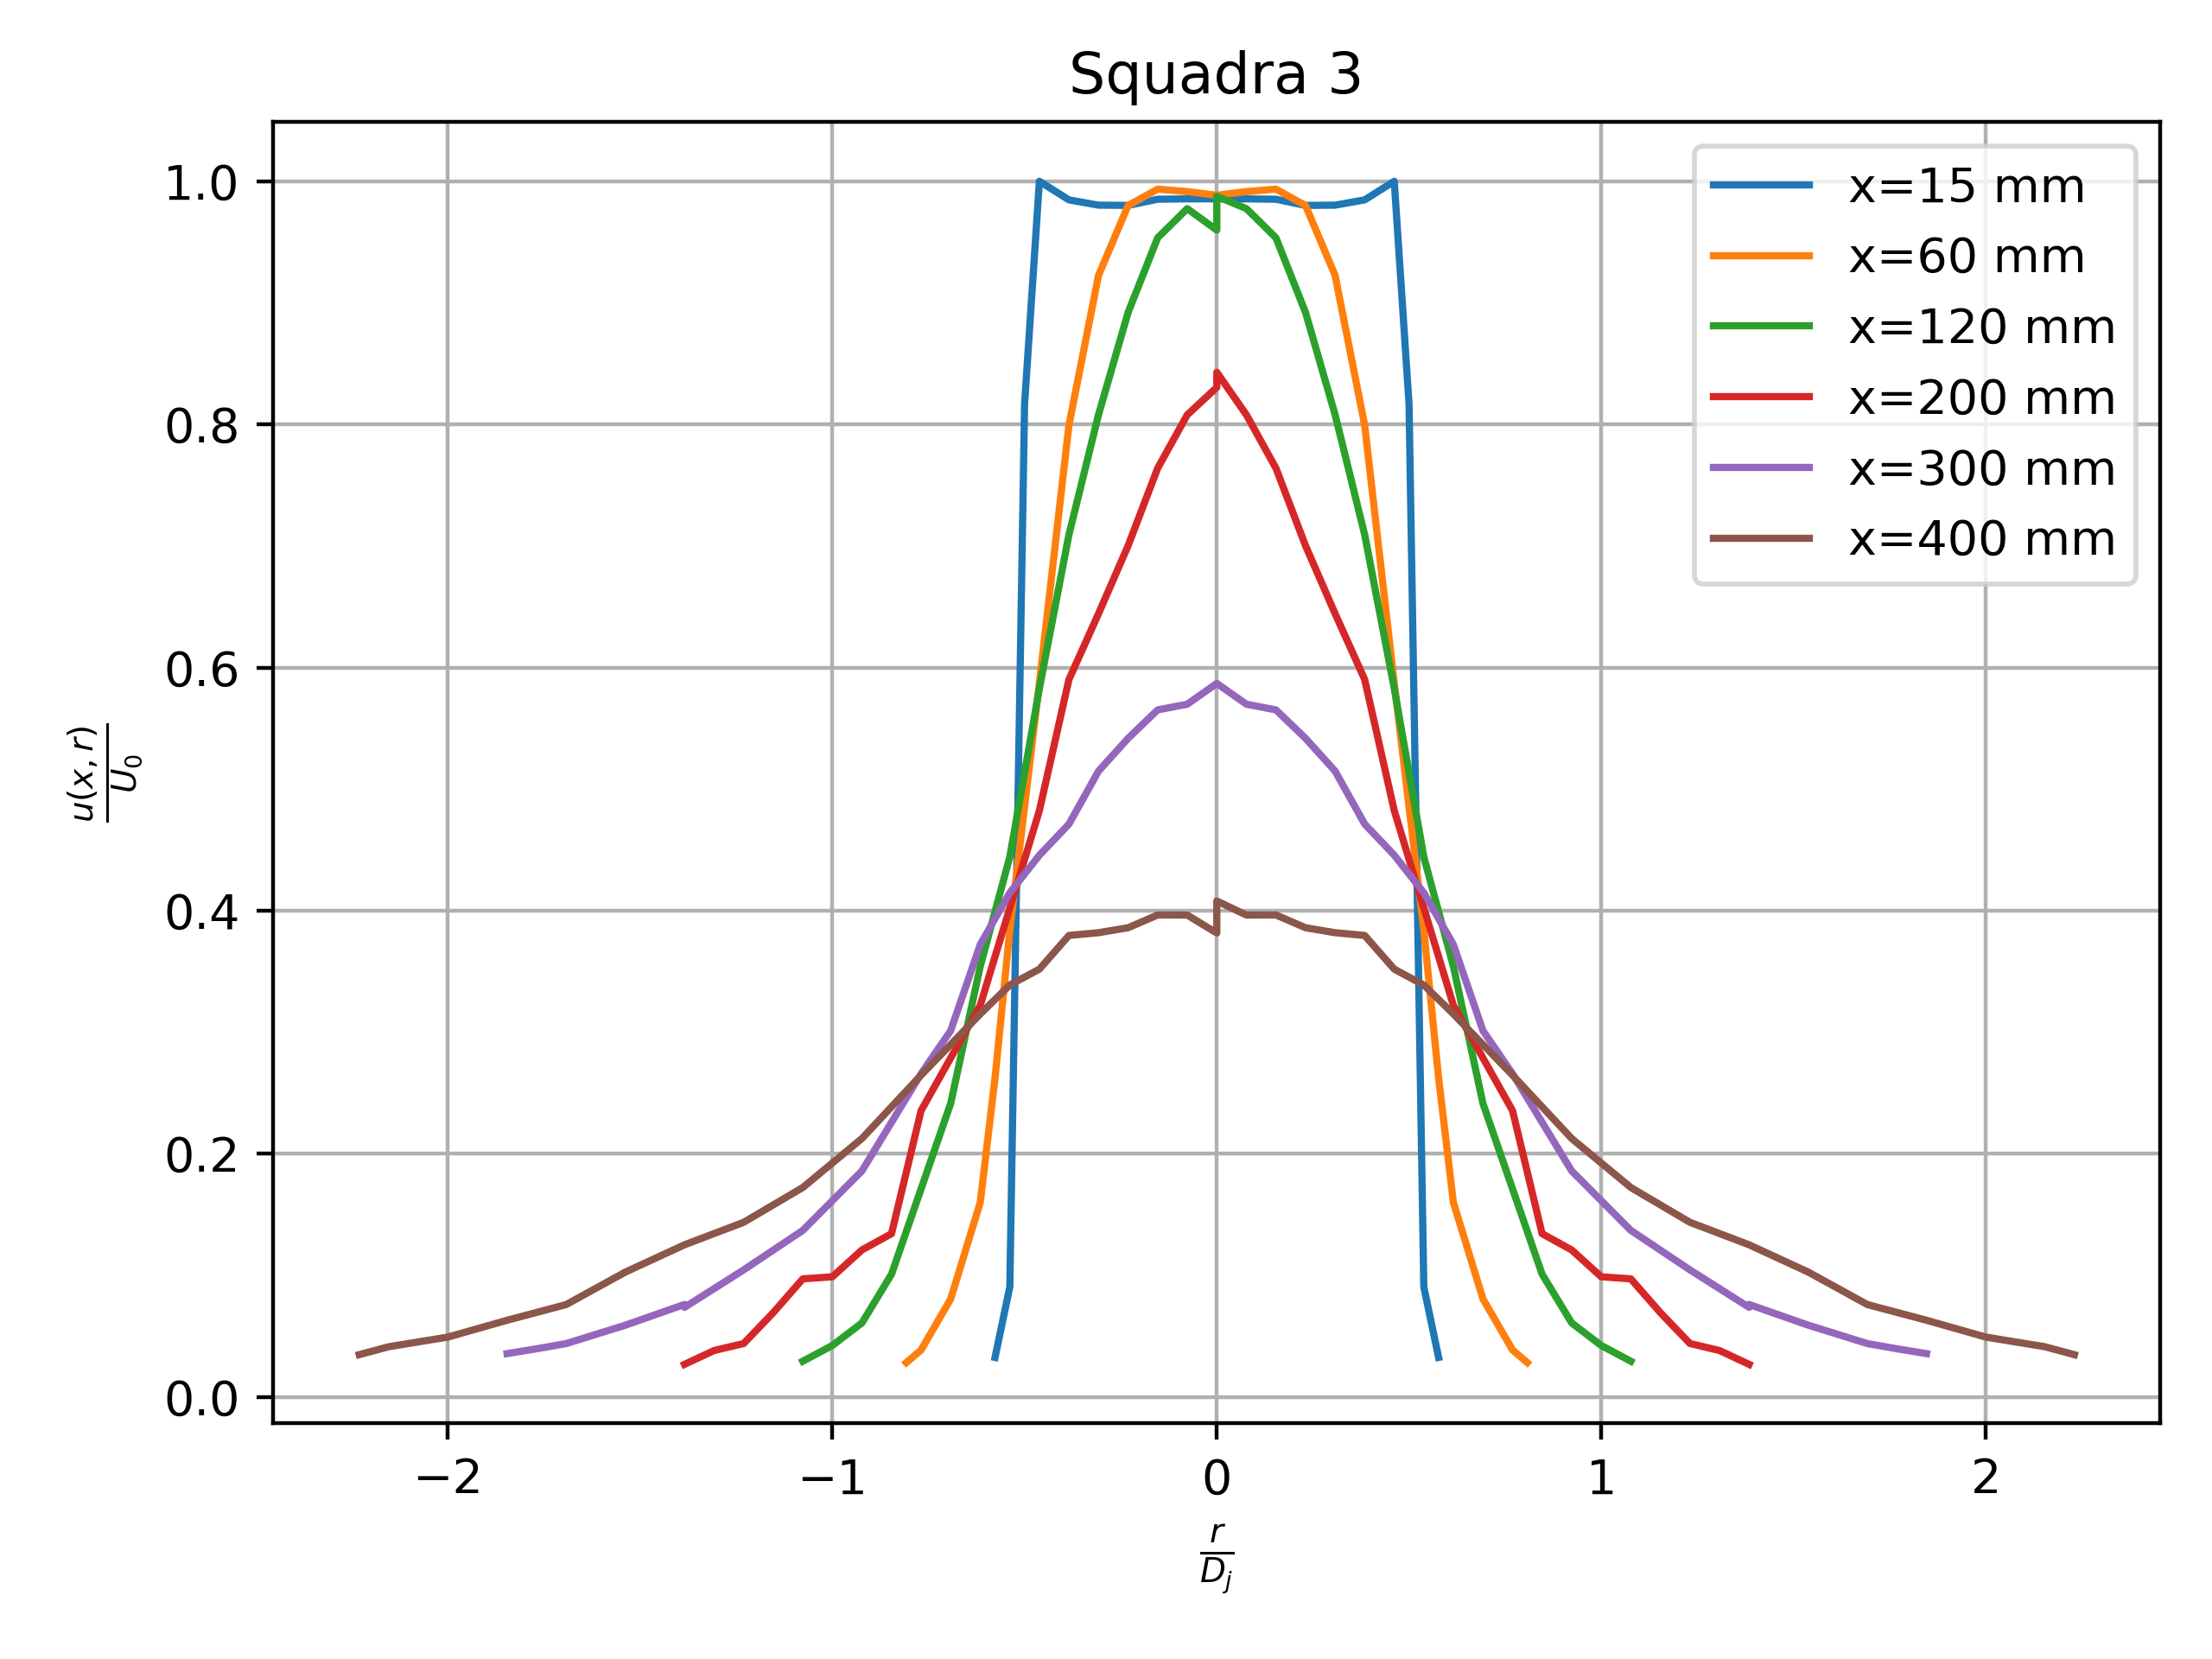
\includegraphics[width=.85\textwidth]{images/3/sq3u0.png}
    \caption{Profili di velocità adimensionali per la terza squadra}
\end{figure}
\begin{figure}[H]
    \centering
    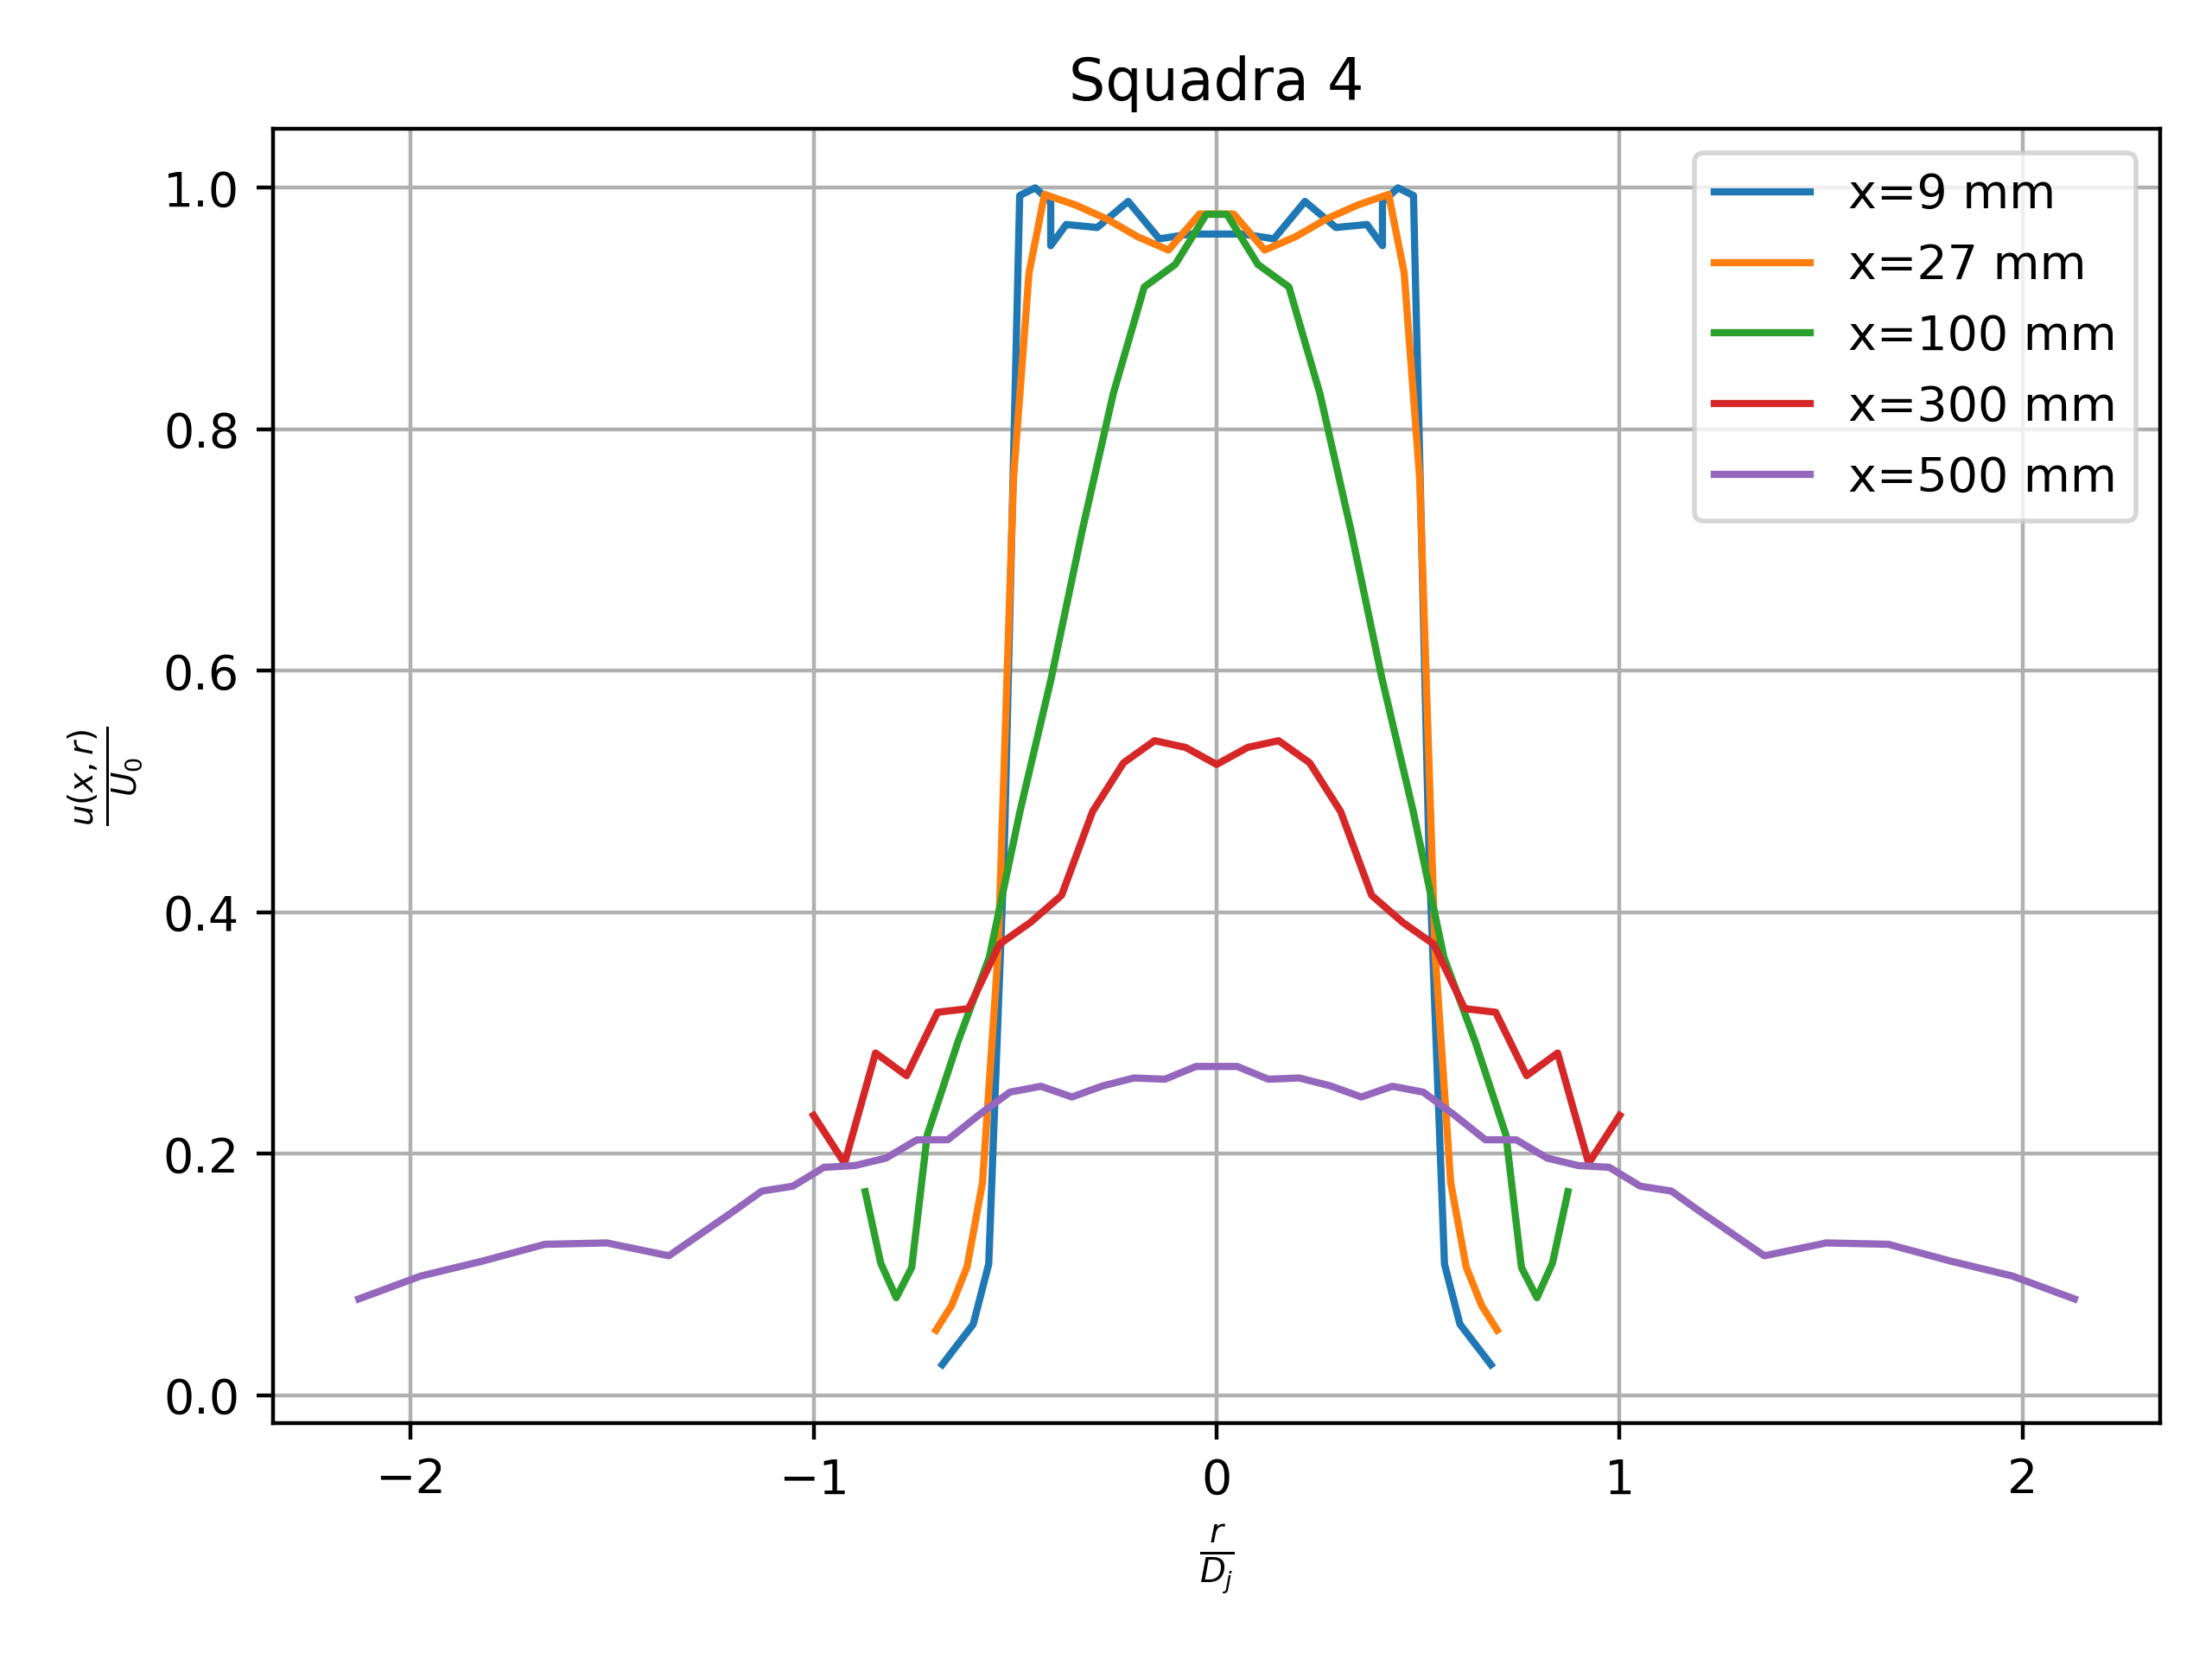
\includegraphics[width=.85\textwidth]{images/3/sq4u0.png}
    \caption{Profili di velocità adimensionali per la quarta squadra}
\end{figure}

\noindent Un ulteriore modo per diagrammare i profili di velocità adimensionali è quello di utilizzare la velocità massima locale e la dimensione trasversale del getto locale per normalizzare la velocità e la distanza radiale:
\begin{equation*}
    \frac{U(x,r)}{U_{max}(x)} = \frac{r}{r_{U=0.5U_{max}}(x)}
\end{equation*}
Il calcolo della velocità massima locale è immediato, per quanto riguarda invece la dimensione trasversale questa si calcola interpolando il valore di $r$ tale per cui la velocità è pari alla metà della velocità massima locale. Si ottengono quindi i seguenti diagrammi:
\begin{figure}[H]
    \centering
    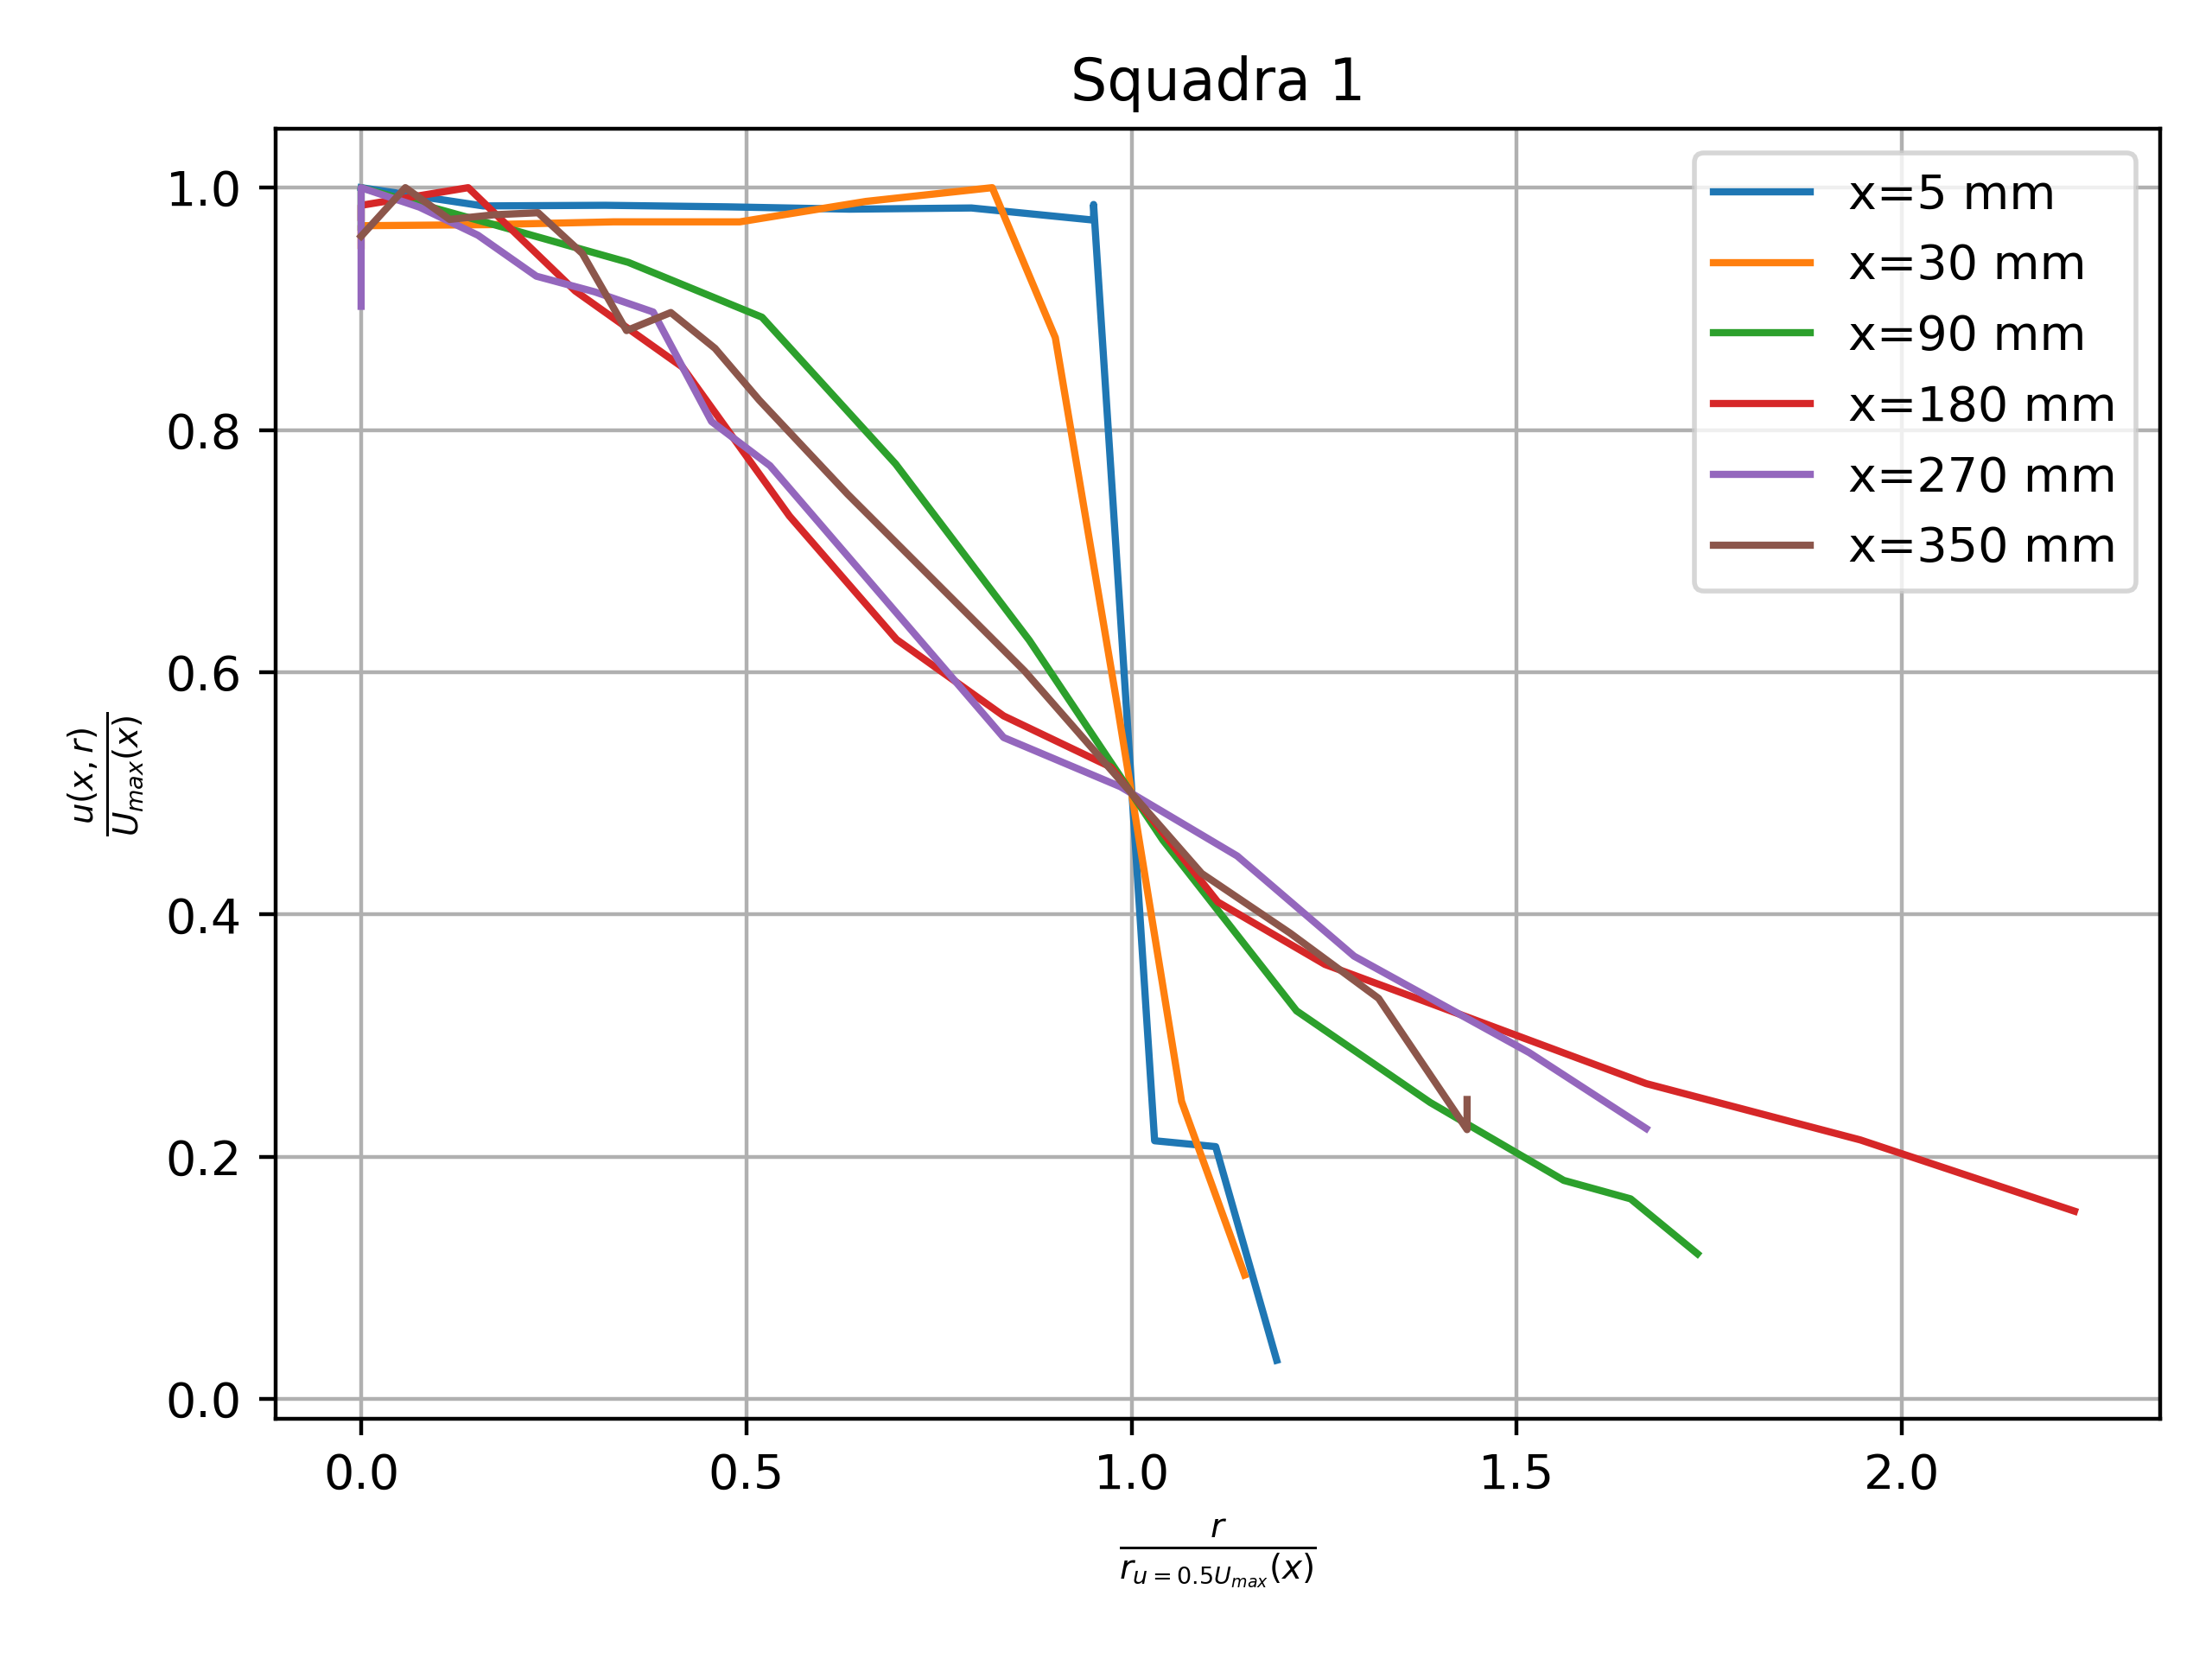
\includegraphics[width=.7\textwidth]{images/3/sq1umax.png}
    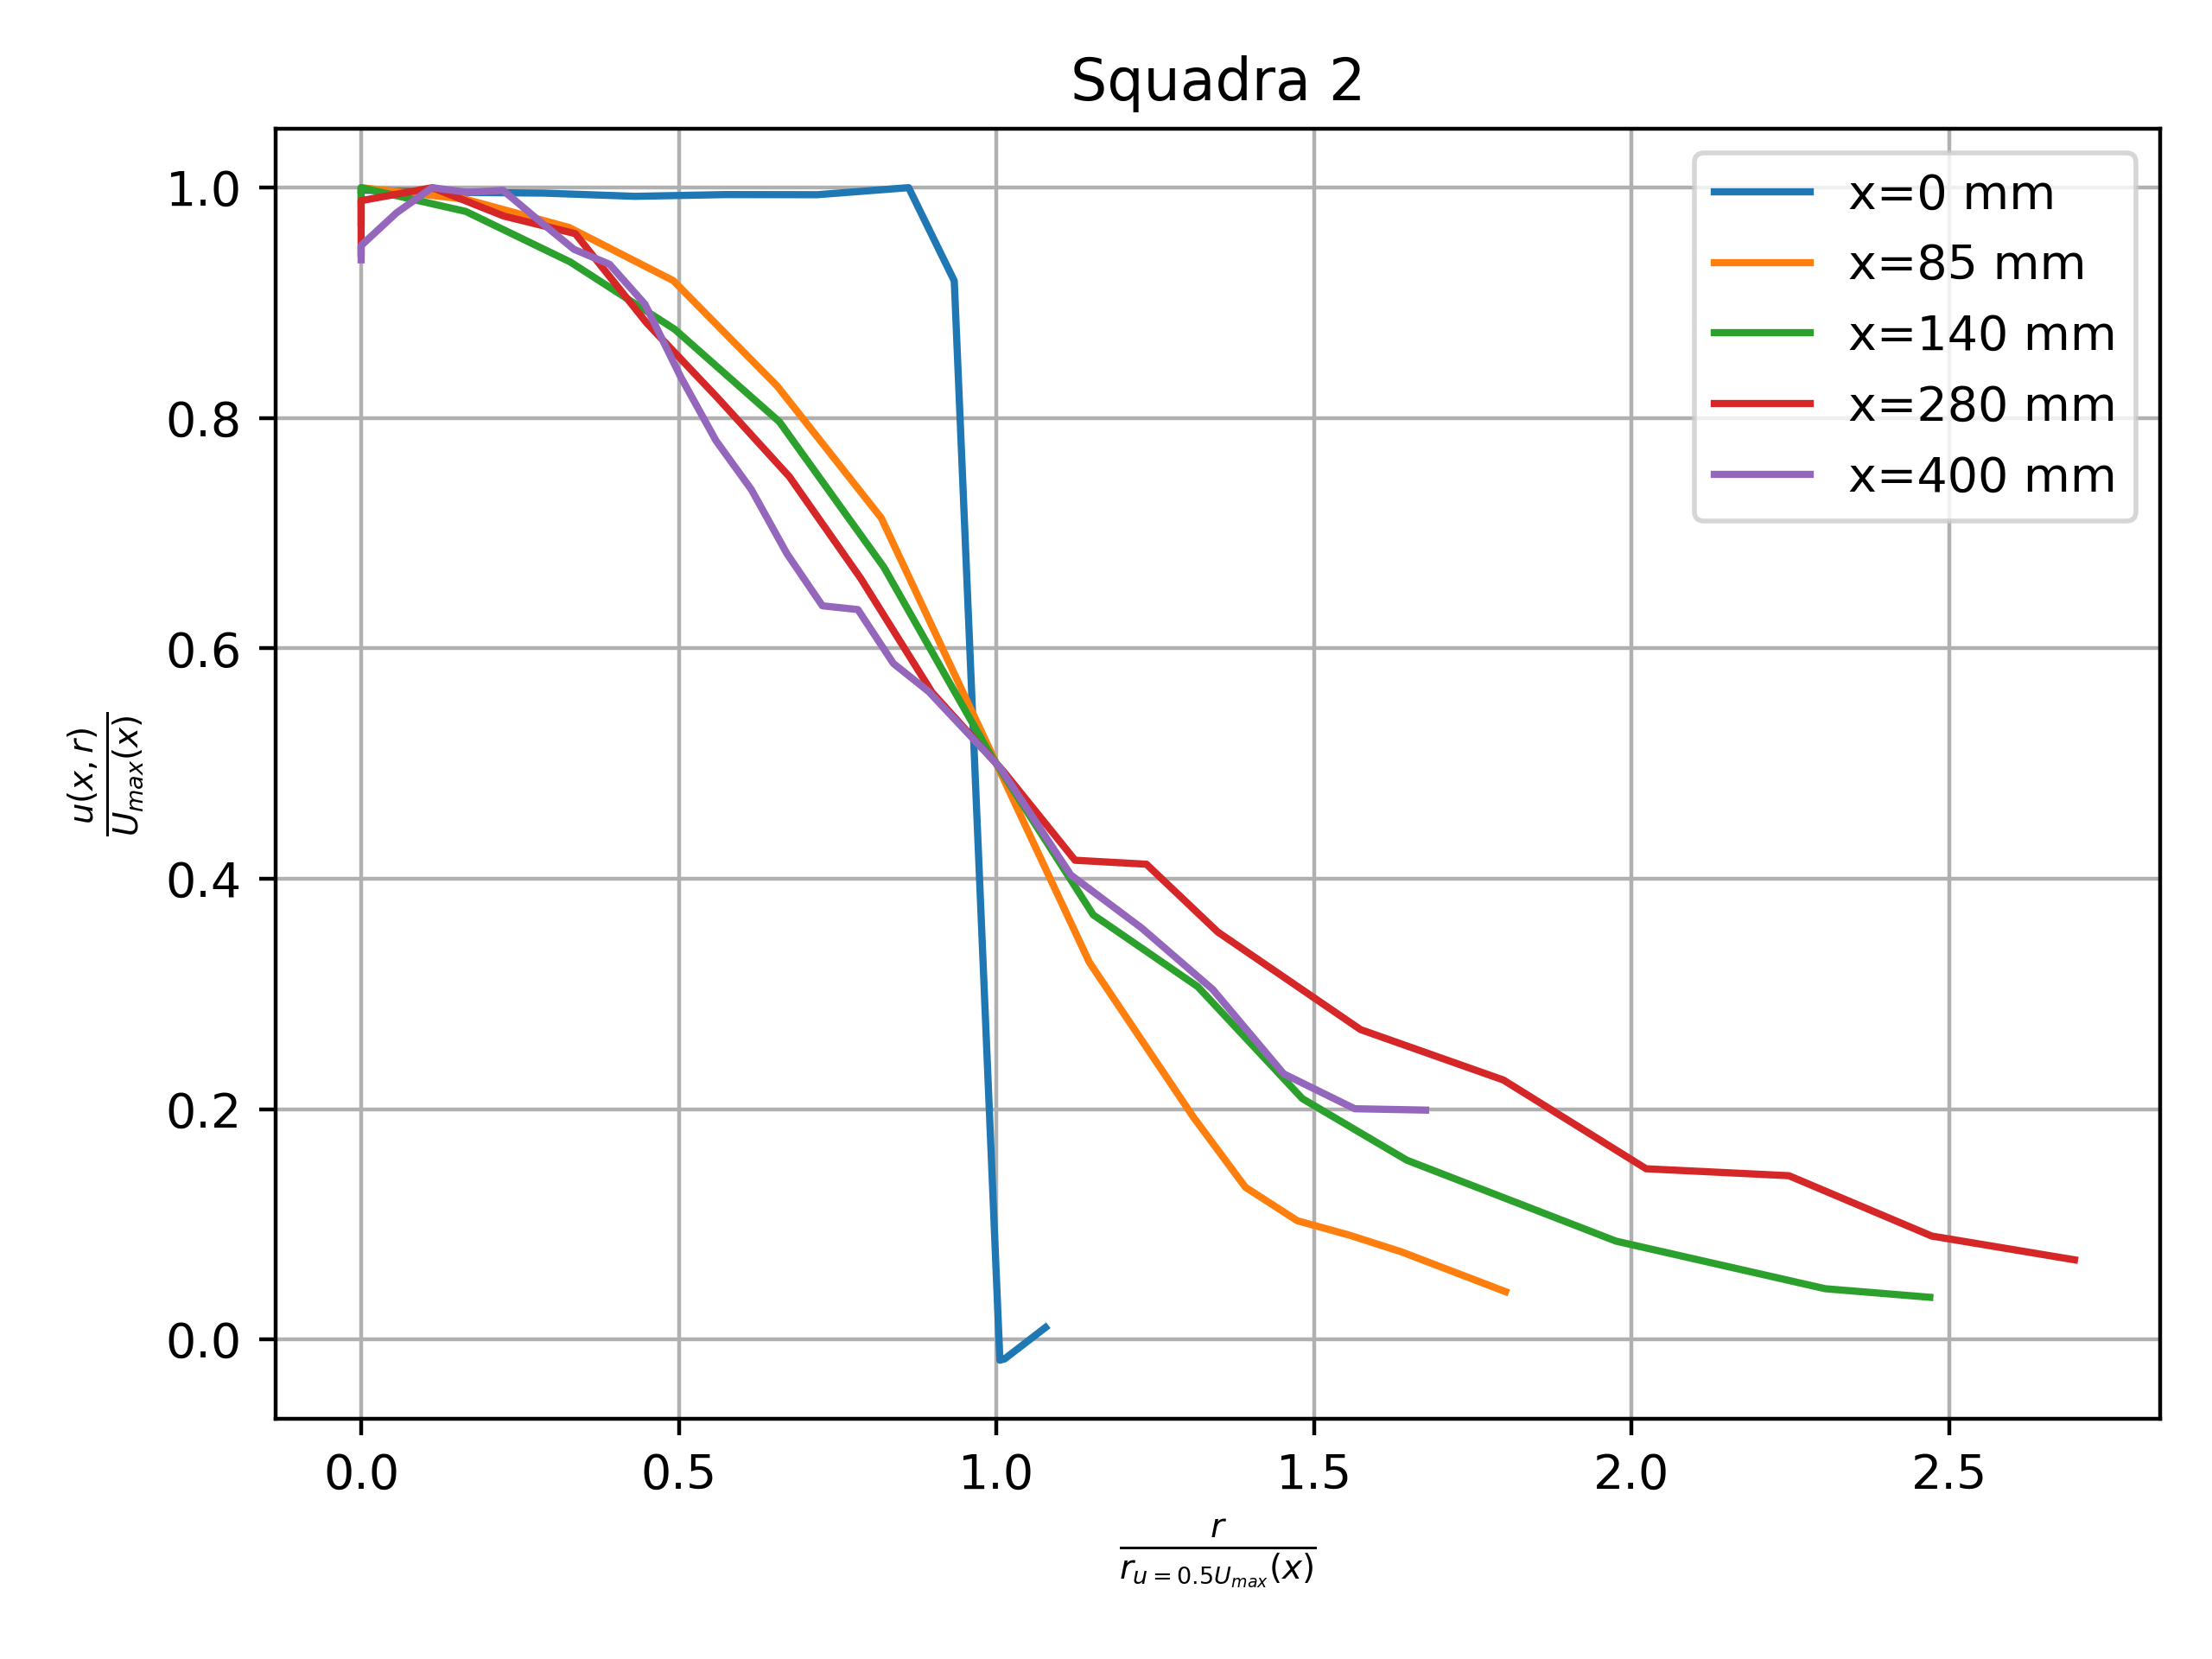
\includegraphics[width=.7\textwidth]{images/3/sq2umax.png}
    \caption{Profili di velocità adimensionali per la prima e per la seconda squadra}
\end{figure}
\begin{figure}[H]
    \centering
    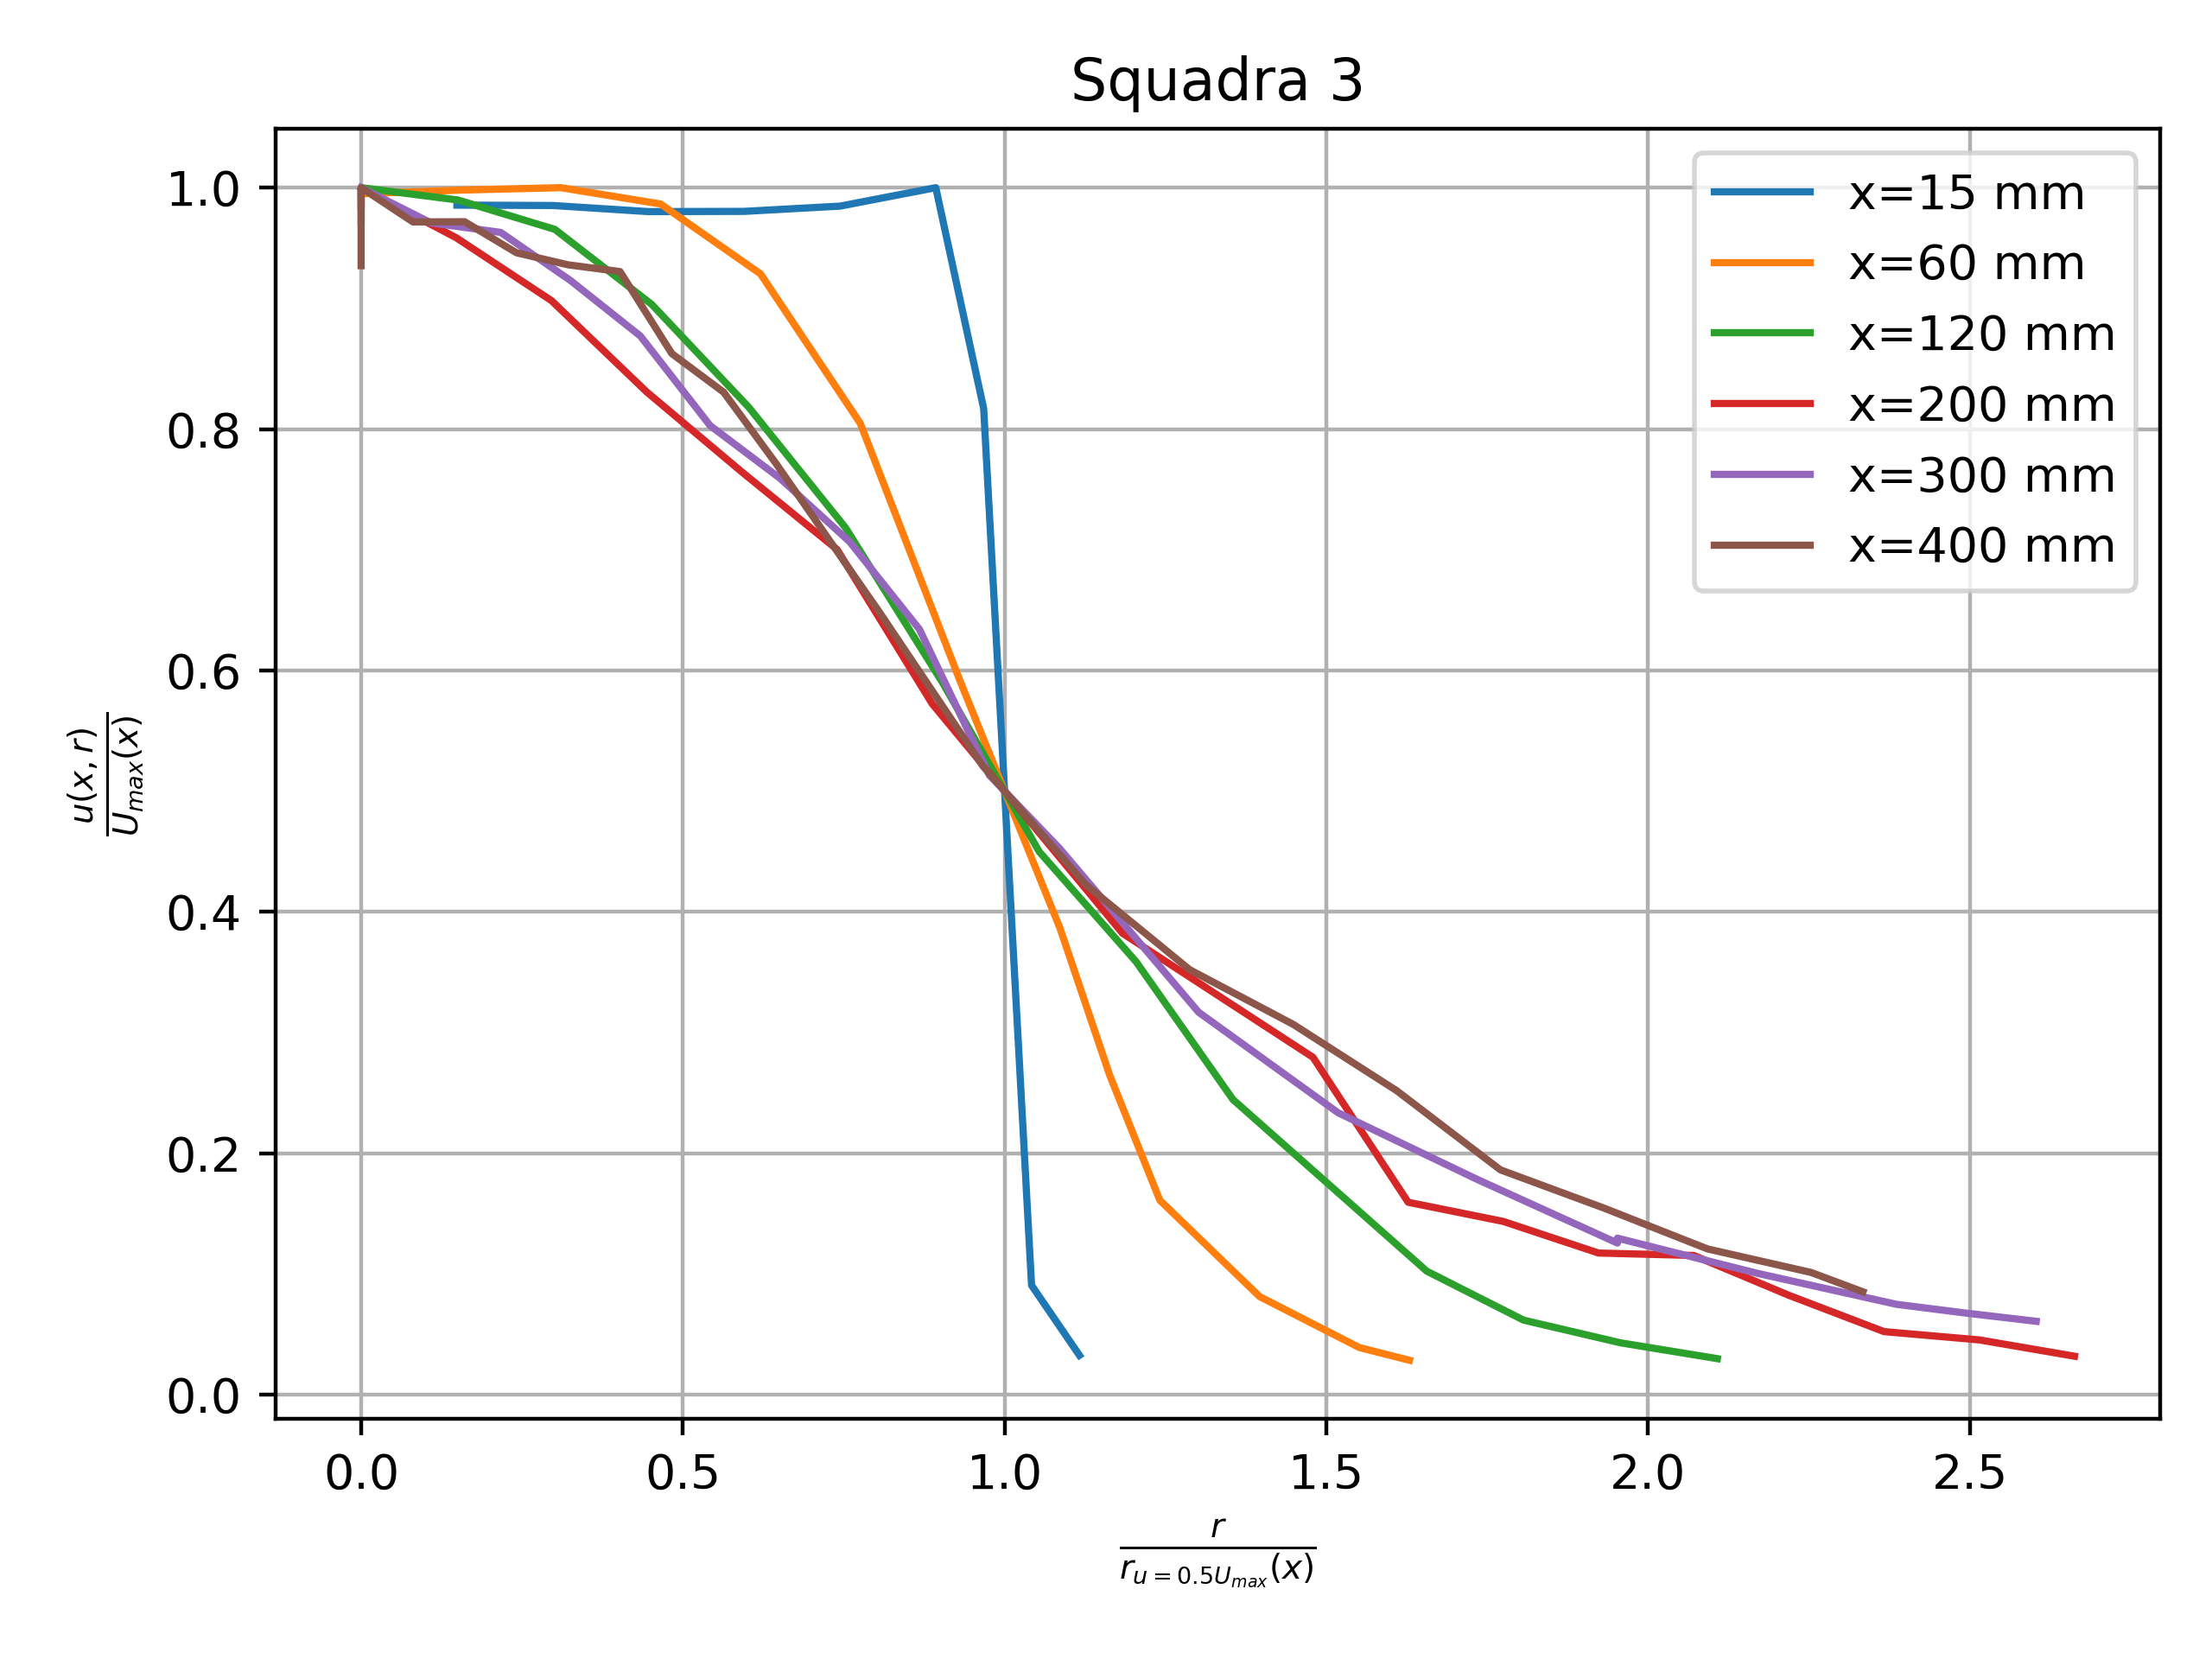
\includegraphics[width=.8\textwidth]{images/3/sq3umax.png}
    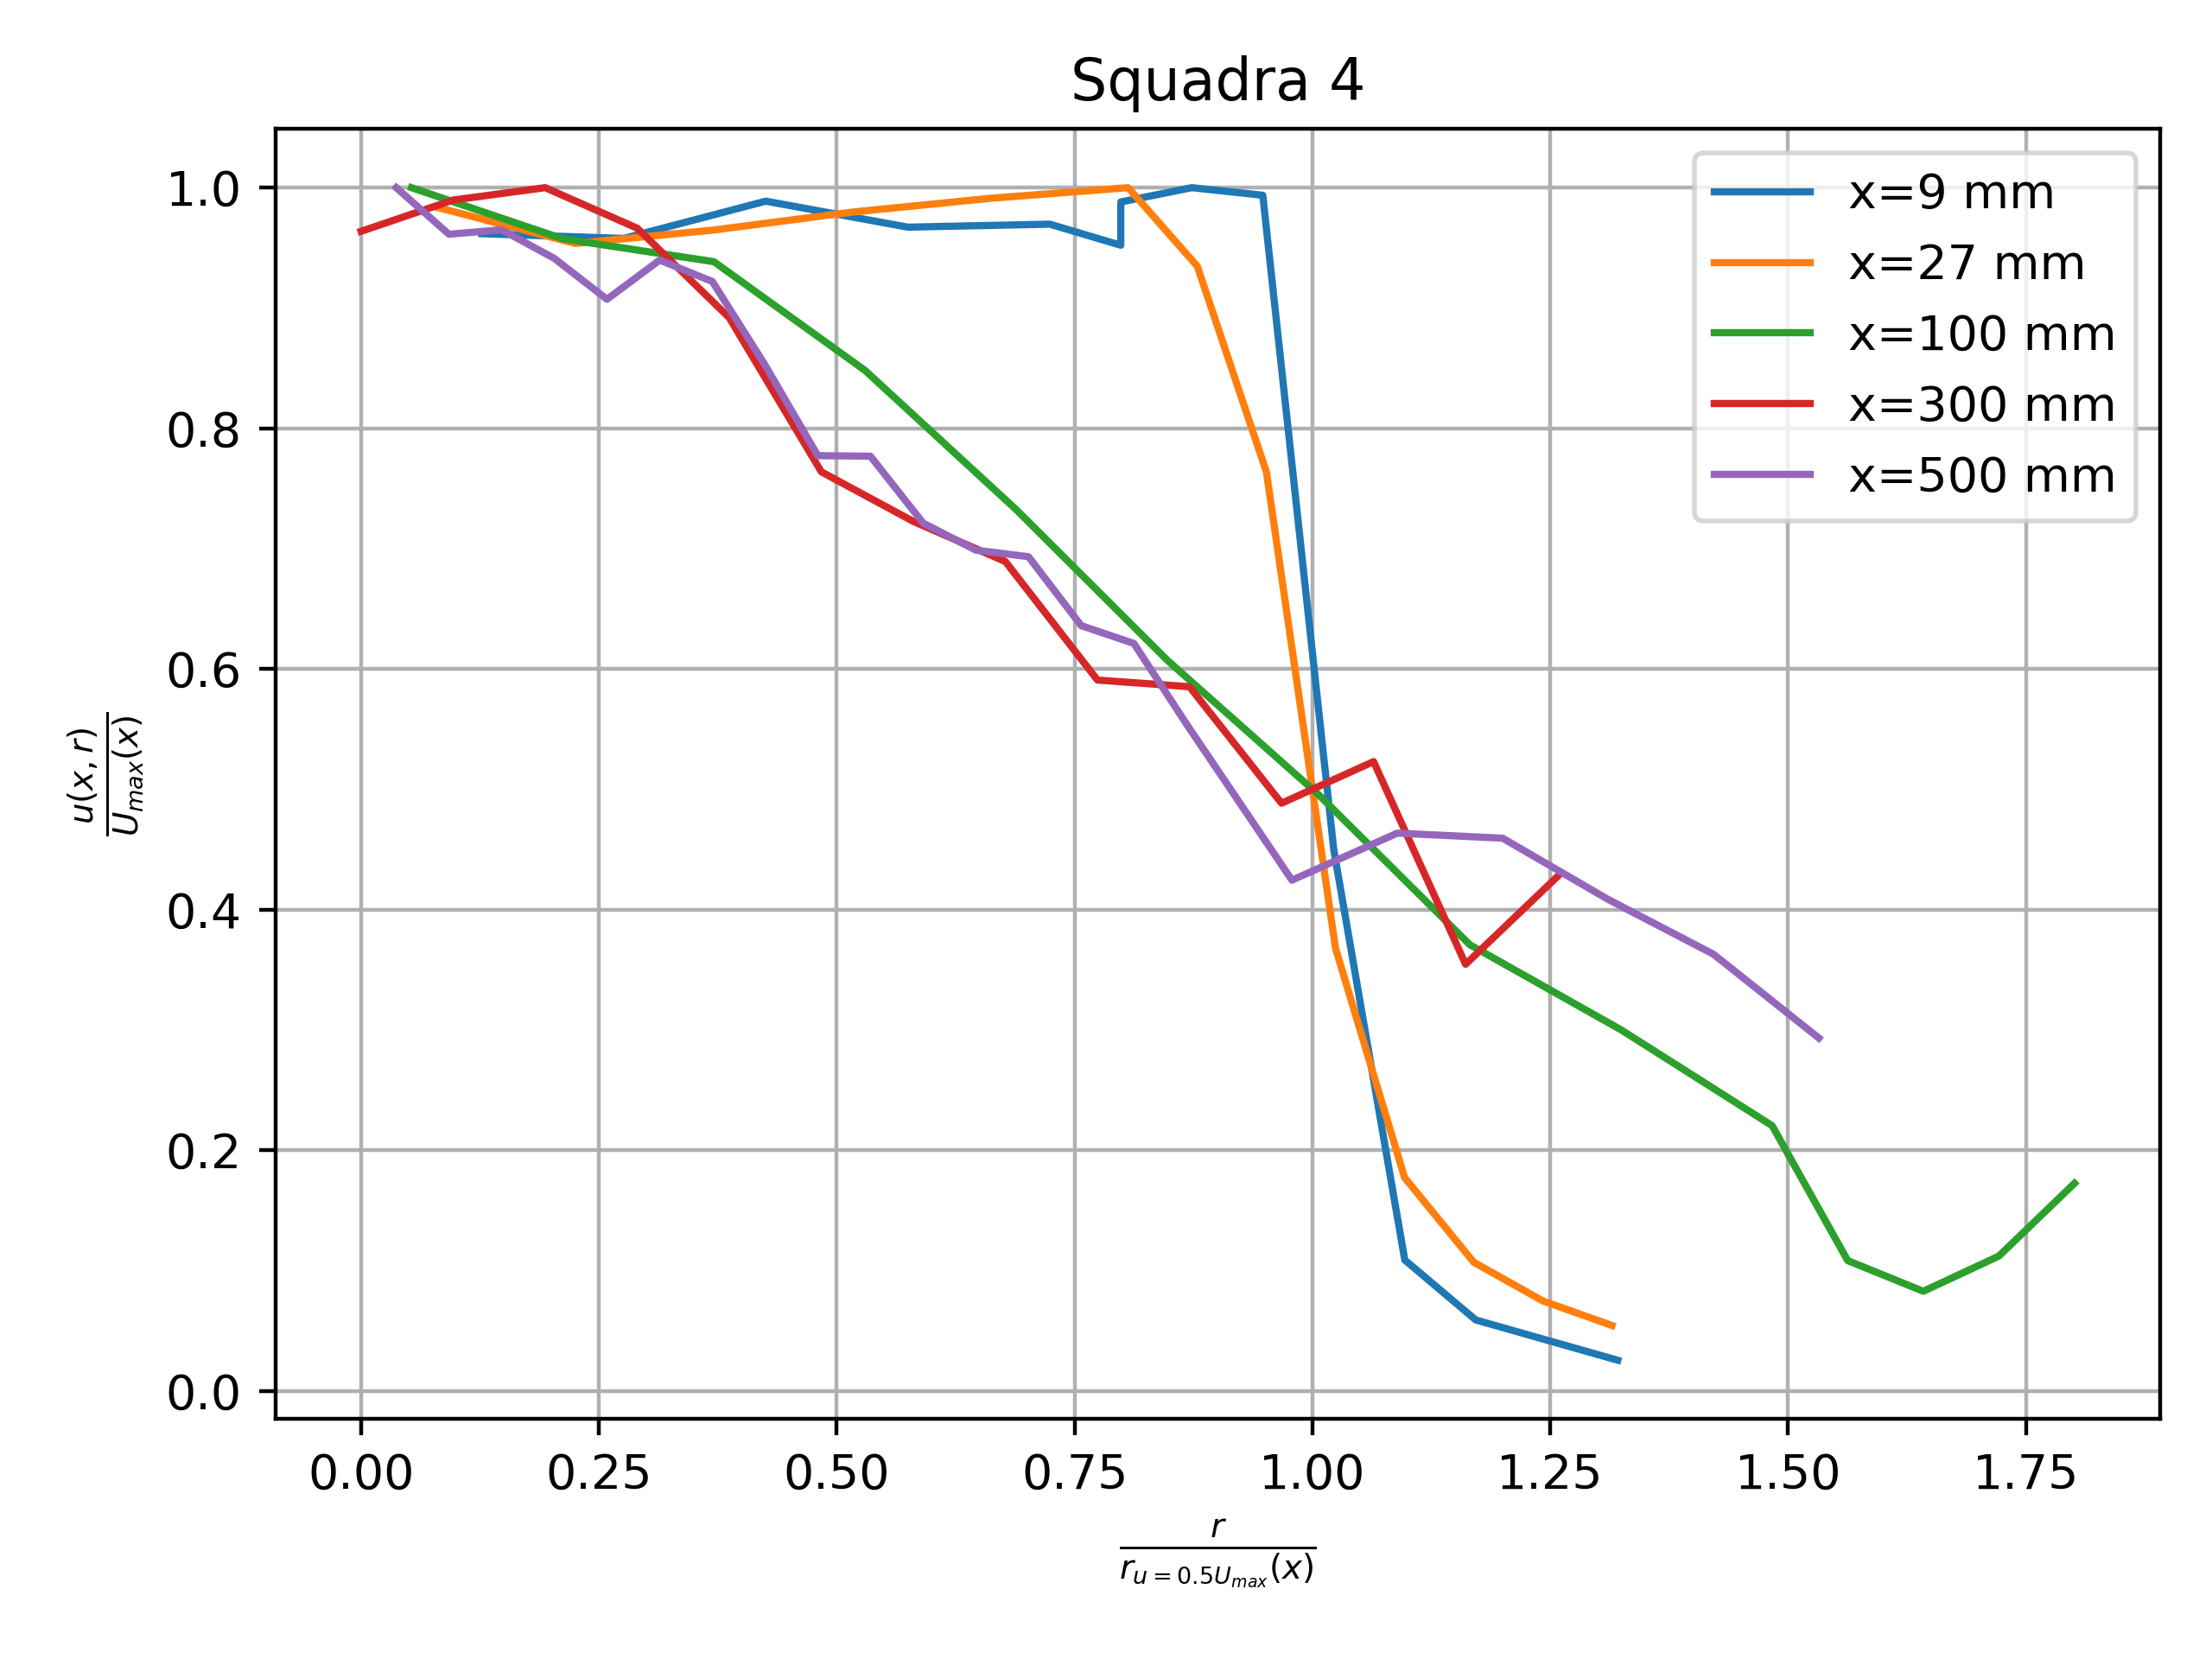
\includegraphics[width=.8\textwidth]{images/3/sq4umax.png}
    \caption{Profili di velocità adimensionali per la terza e per la quarta squadra}
\end{figure}

\noindent Così come accennato in precedenza, dai risultati ottenuti si osserva come nella regione autosimilare i profili di velocità adimensionali tendono a sovrapporsi.
\section{Proprietà del getto}
Sulla base delle misure e dei profili di velocità media, effettuate al variare della distanza $x$ dalla sezione di uscita e del numero di Reynolds (portata del getto), si valutano gli andamenti di altre proprietà del getto una volta evidenziate le regioni caratteristiche nella precedente esercitazione.\\\\
In particolare, si vogliono valutare:
\begin{itemize}
    \item La velocità massima $U_{max}(x)$;
    \item La dimensione trasversale del getto $\Delta(x)$;
    \item La portata in massa $G(x)$;
    \item La quantità di moto $M(x)$;
    \item L'energia $E(x)$.
\end{itemize}
L'analisi dati per la presente attività è condotta con l'ausilio di un codice Python, riportato in appendice \ref{b4}.

\subsection{Velocità massima}
La velocità massima del getto per ogni profilo di velocità misurato risulta essere in prossimità dell'asse del getto. Si può quindi diagrammare l'andamento della velocità massima $U_{max}(x)$ in funzione della distanza assiale $x$.\\\\
Si evidenzia il noto risultato teorico per la velocità massima nella regione self-similare:
\begin{equation*}
    \frac{U_{max}(x)}{U_0} = \frac{k}{(x/D)^m}
\end{equation*}
dove $k$ ed $m$ sono costanti da determinare sperimentalmente.\\\\
Rimaneggiando tale relazione, si ottiene:
\begin{equation*}
    \log \frac{U_{max}(x)}{U_0} = -m \log\frac{x}{D_j} + \log k
\end{equation*}
Imponendo le seguenti sostituzioni:
\begin{equation*}
    y = \log \frac{U_{max}(x)}{U_0} \qquad x = \log\frac{x}{D_j} \qquad q = \log k
\end{equation*}
si evidenzia l'equazione di una retta:
\begin{equation*}
    y = -mx + q
\end{equation*}
Con una semplice interpolazione lineare dei dati nella regione autosimilare è dunque possibile ricavare i valori di $m$ e $k$ per le quattro squadre, si ottiene:
\begin{equation*}
    \begin{split}
        \text{Squadra 1: } m = 1.346 &\quad k = 8.377\\
        \text{Squadra 2: } m = 1.268 &\quad k = 8.368\\
        \text{Squadra 3: } m = 1.037 &\quad k = 7.110\\
        \text{Squadra 4: } m = 1.292 &\quad k = 12.781
    \end{split}
\end{equation*}
Utilizzando i valori di velocità massima per le quattro squadre, si ricava il seguente diagramma:
\begin{figure}[h]
    \centering
    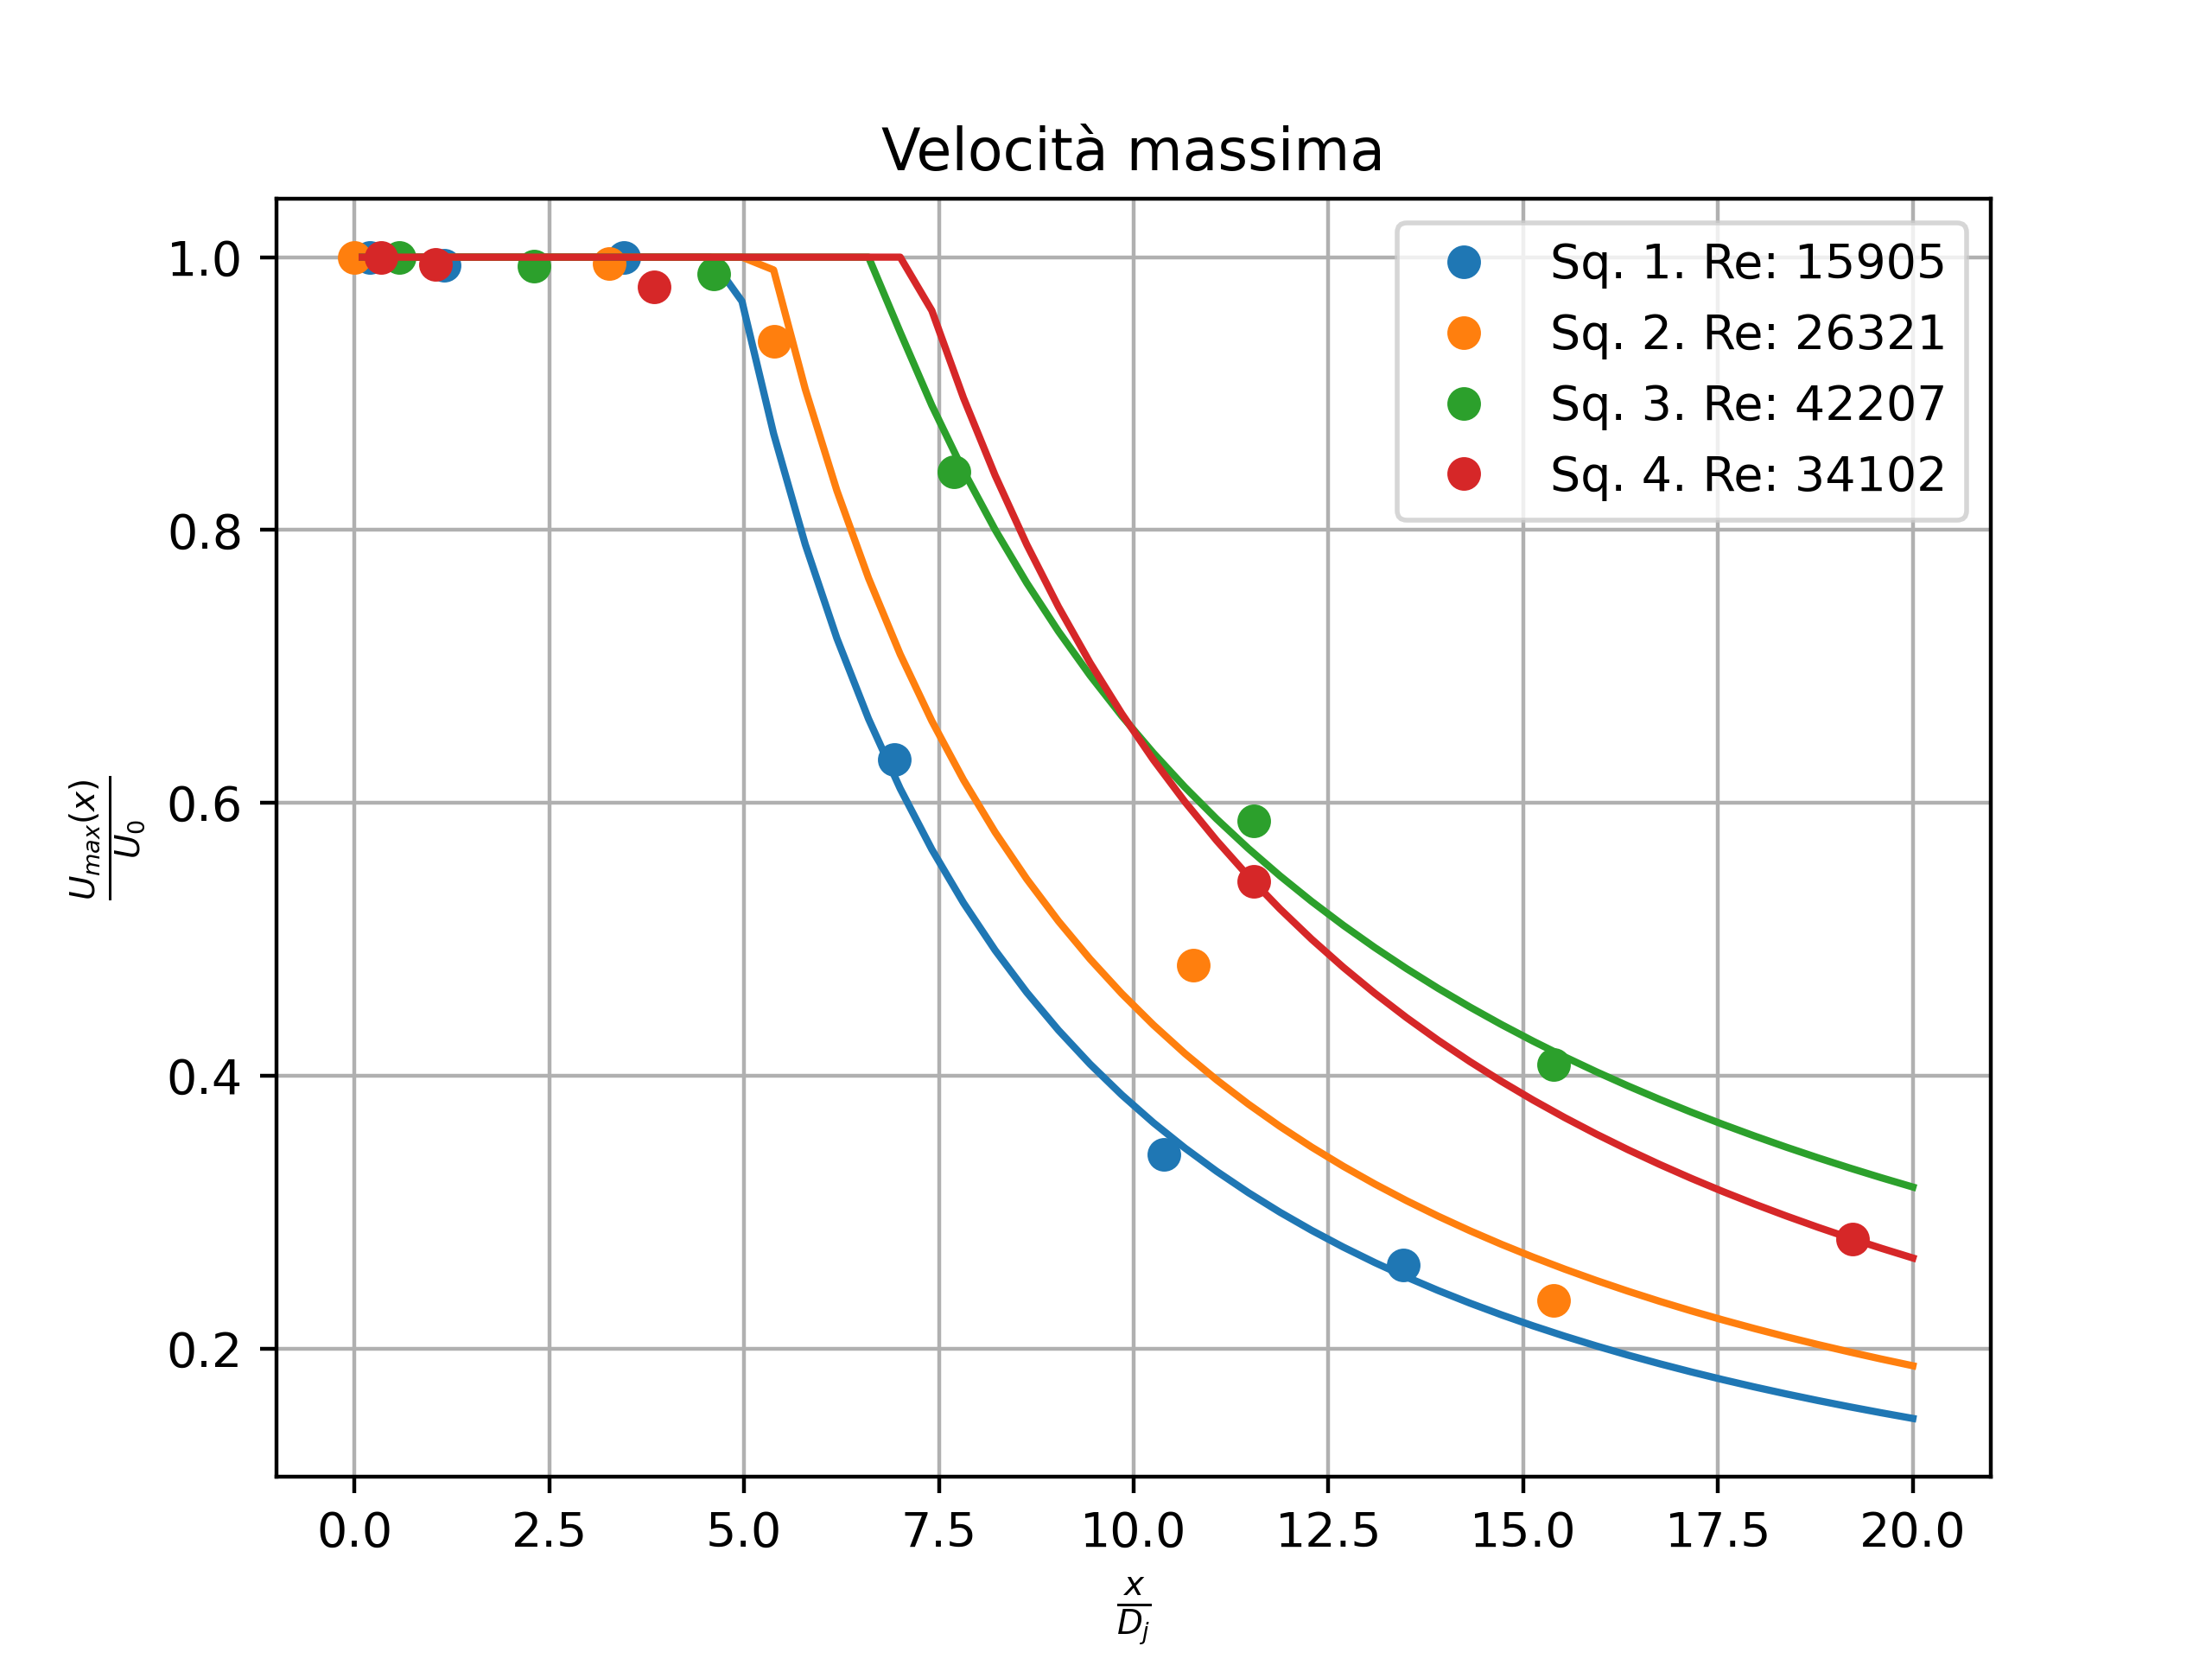
\includegraphics[width=.9\textwidth]{images/4/umax.png}
    \caption{Velocità massima lungo l'asse del getto}
\end{figure}

\noindent Il primo tratto costante evidenzia il cuore potenziale del getto, seguito dall'andamento esponenziale appena ricavato.\\\\
Si nota l'influenza del numero di Reynolds, infatti all'aumentare del numero di Reynolds aumenta la lunghezza assiale del cuore potenziale del getto, mentre nella regione self-similare per i quattro flussi analizzati la velocità massima decresce con un esponente $m$ che sembra non variare significativamente.

\subsection{Dimensione trasversale del getto}
Il getto trascina nel suo moto una quantità sempre crescente di fluido esterno a causa degli effetti viscosi (entrainment), quindi aumenta di spessore lungo l'asse.\\\\
La dimensione trasversale del getto è arbitrariamente definita come il valore di $r$ tale per cui la velocità è pari alla metà della velocità massima locale:
\begin{equation*}
    \Delta (x) = r_{U=0.5U_{max}(x)}
\end{equation*}
Si ottiene il seguente diagramma per le quattro squadre:
\begin{figure}[H]
    \centering
    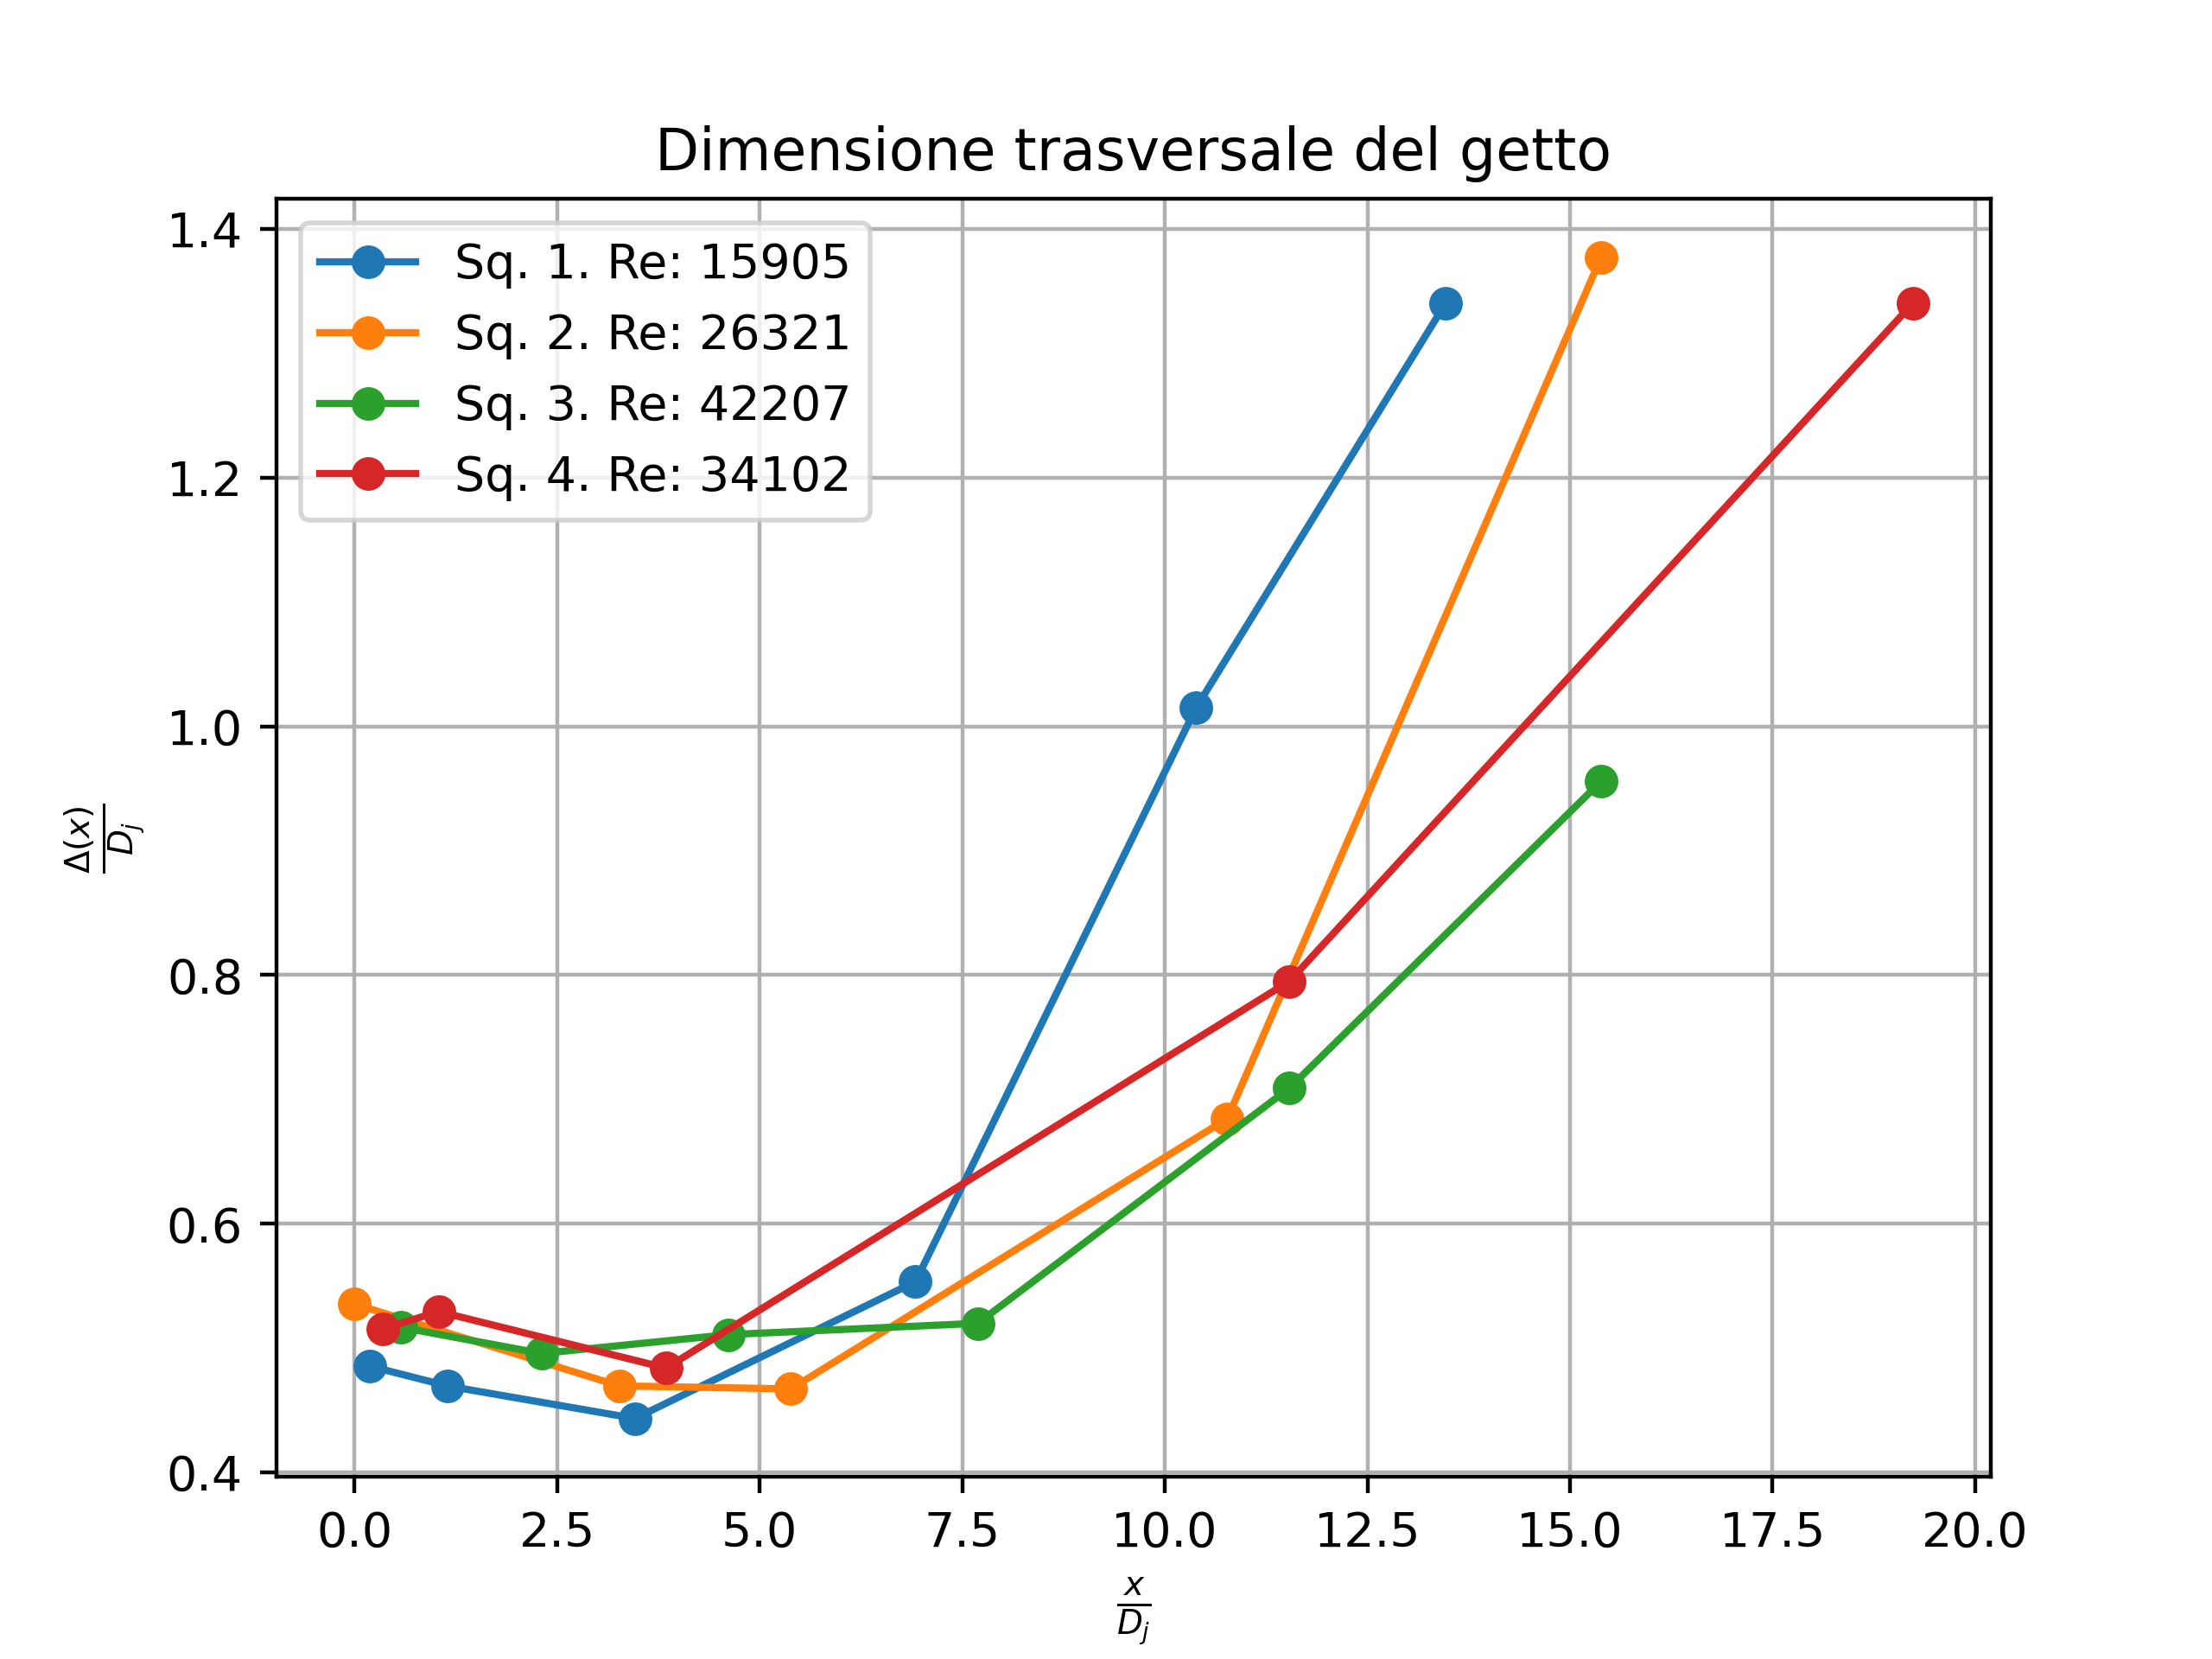
\includegraphics[width=.7\textwidth]{images/4/delta.png}
    \caption{Dimensione trasversale del getto}
\end{figure}
\begin{figure}[H]
    \centering
    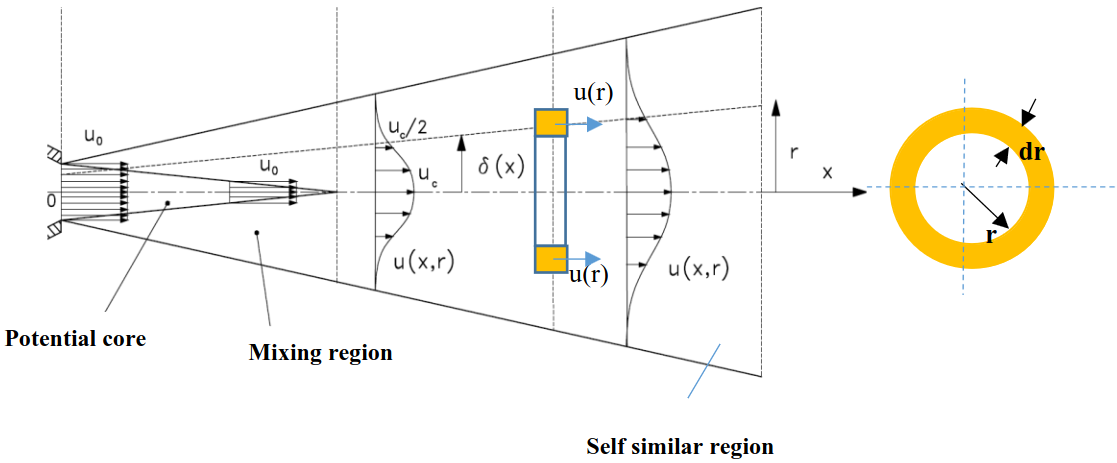
\includegraphics[width=.8\linewidth]{images/4/getto.png}
    \caption{Rappresentazione del getto}
\end{figure}

\subsection{Portata in massa}
A causa del trascinamento (entrainment) operato sul confine esterno del getto è atteso un aumento della portata in massa nella direzione dell'asse.\\\\
La portata elementare è definita come:
\begin{equation*}
    dG = \rho\ u\ dA = \rho\ u\ 2\pi rdr
\end{equation*}
Integrando si ottiene:
\begin{equation*}
    G = 2\pi\rho \int_0^\infty ur dr \quad \left[\frac{kg}{s} \right]
\end{equation*}
La portata in massa in corrispondenza della sezione di uscita è invece:
\begin{equation*}
    G_0 = \rho \left( \frac{\pi D^2}4 \right) U_0
\end{equation*}
Valutando la funzione integranda in modo discreto utilizzando i dati sperimentali, è possibile risolvere l'integrale con l'applicazione della regola dei trapezi.\\\\
Diagrammando l'andamento della portata $G$, normalizzata rispetto alla portata in corrispondenza della sezione di uscita $G_0$, si ottiene il seguente diagramma:
\begin{figure}[h]
    \centering
    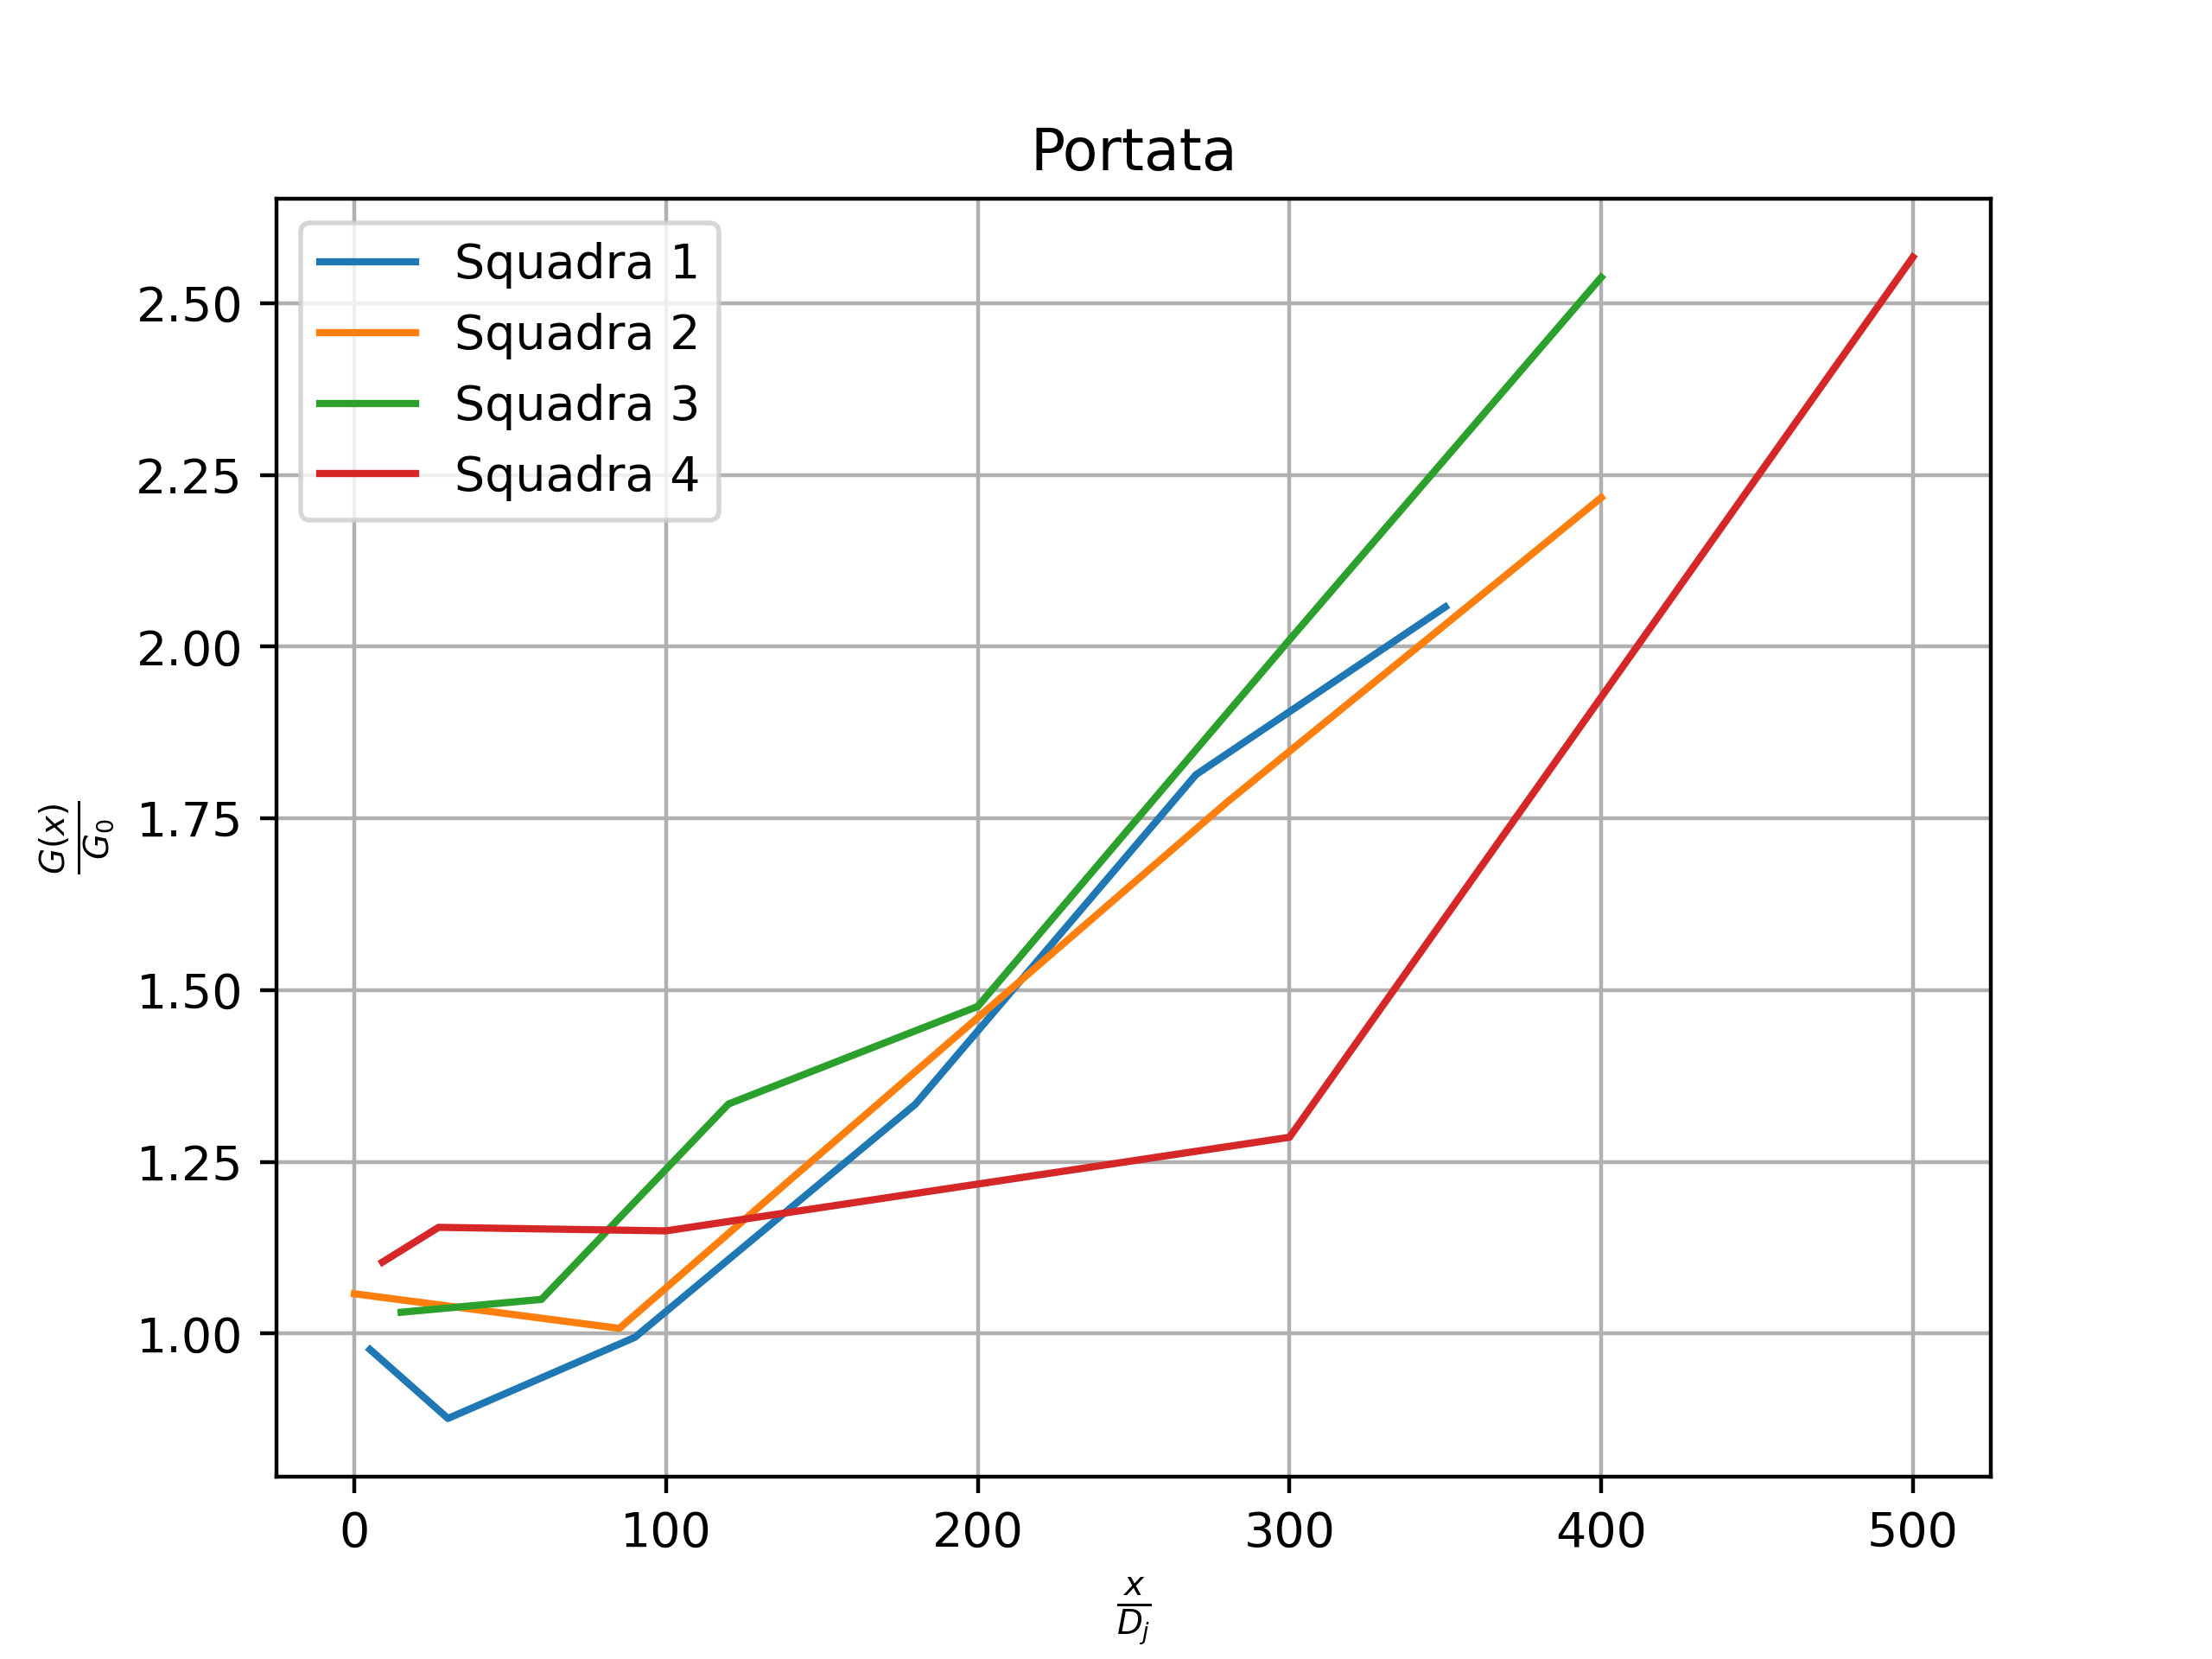
\includegraphics[width=.8\linewidth]{images/4/portata.png}
    \caption{Portata in massa}
\end{figure}

\subsection{Quantità di moto}
Poiché non sono agenti forze esterne sul flusso, è atteso che la quantità di moto lungo l'asse del getto rimanga costante.\\\\
La quantità di moto elementare è definita come:
\begin{equation*}
    dM = dG\ u = 2\pi\rho u^2 rdr
\end{equation*}
Integrando si ottiene:
\begin{equation*}
    M = 2\pi\rho \int_0^\infty u^2r dr \quad \left[\frac{kg\,m}{s^2} \right]
\end{equation*}
La quantità di moto in corrispondenza della sezione di uscita è invece:
\begin{equation*}
    M_0 = \rho \left( \frac{\pi D^2}4 \right) U_0^2
\end{equation*}
Valutando la funzione integranda in modo discreto utilizzando i dati sperimentali, è possibile risolvere l'integrale con l'applicazione della regola dei trapezi.\\\\
Diagrammando l'andamento della quantità di moto $M$, normalizzata rispetto al valore in corrispondenza della sezione di uscita $M_0$, si ottiene il seguente diagramma:
\begin{figure}[h]
    \centering
    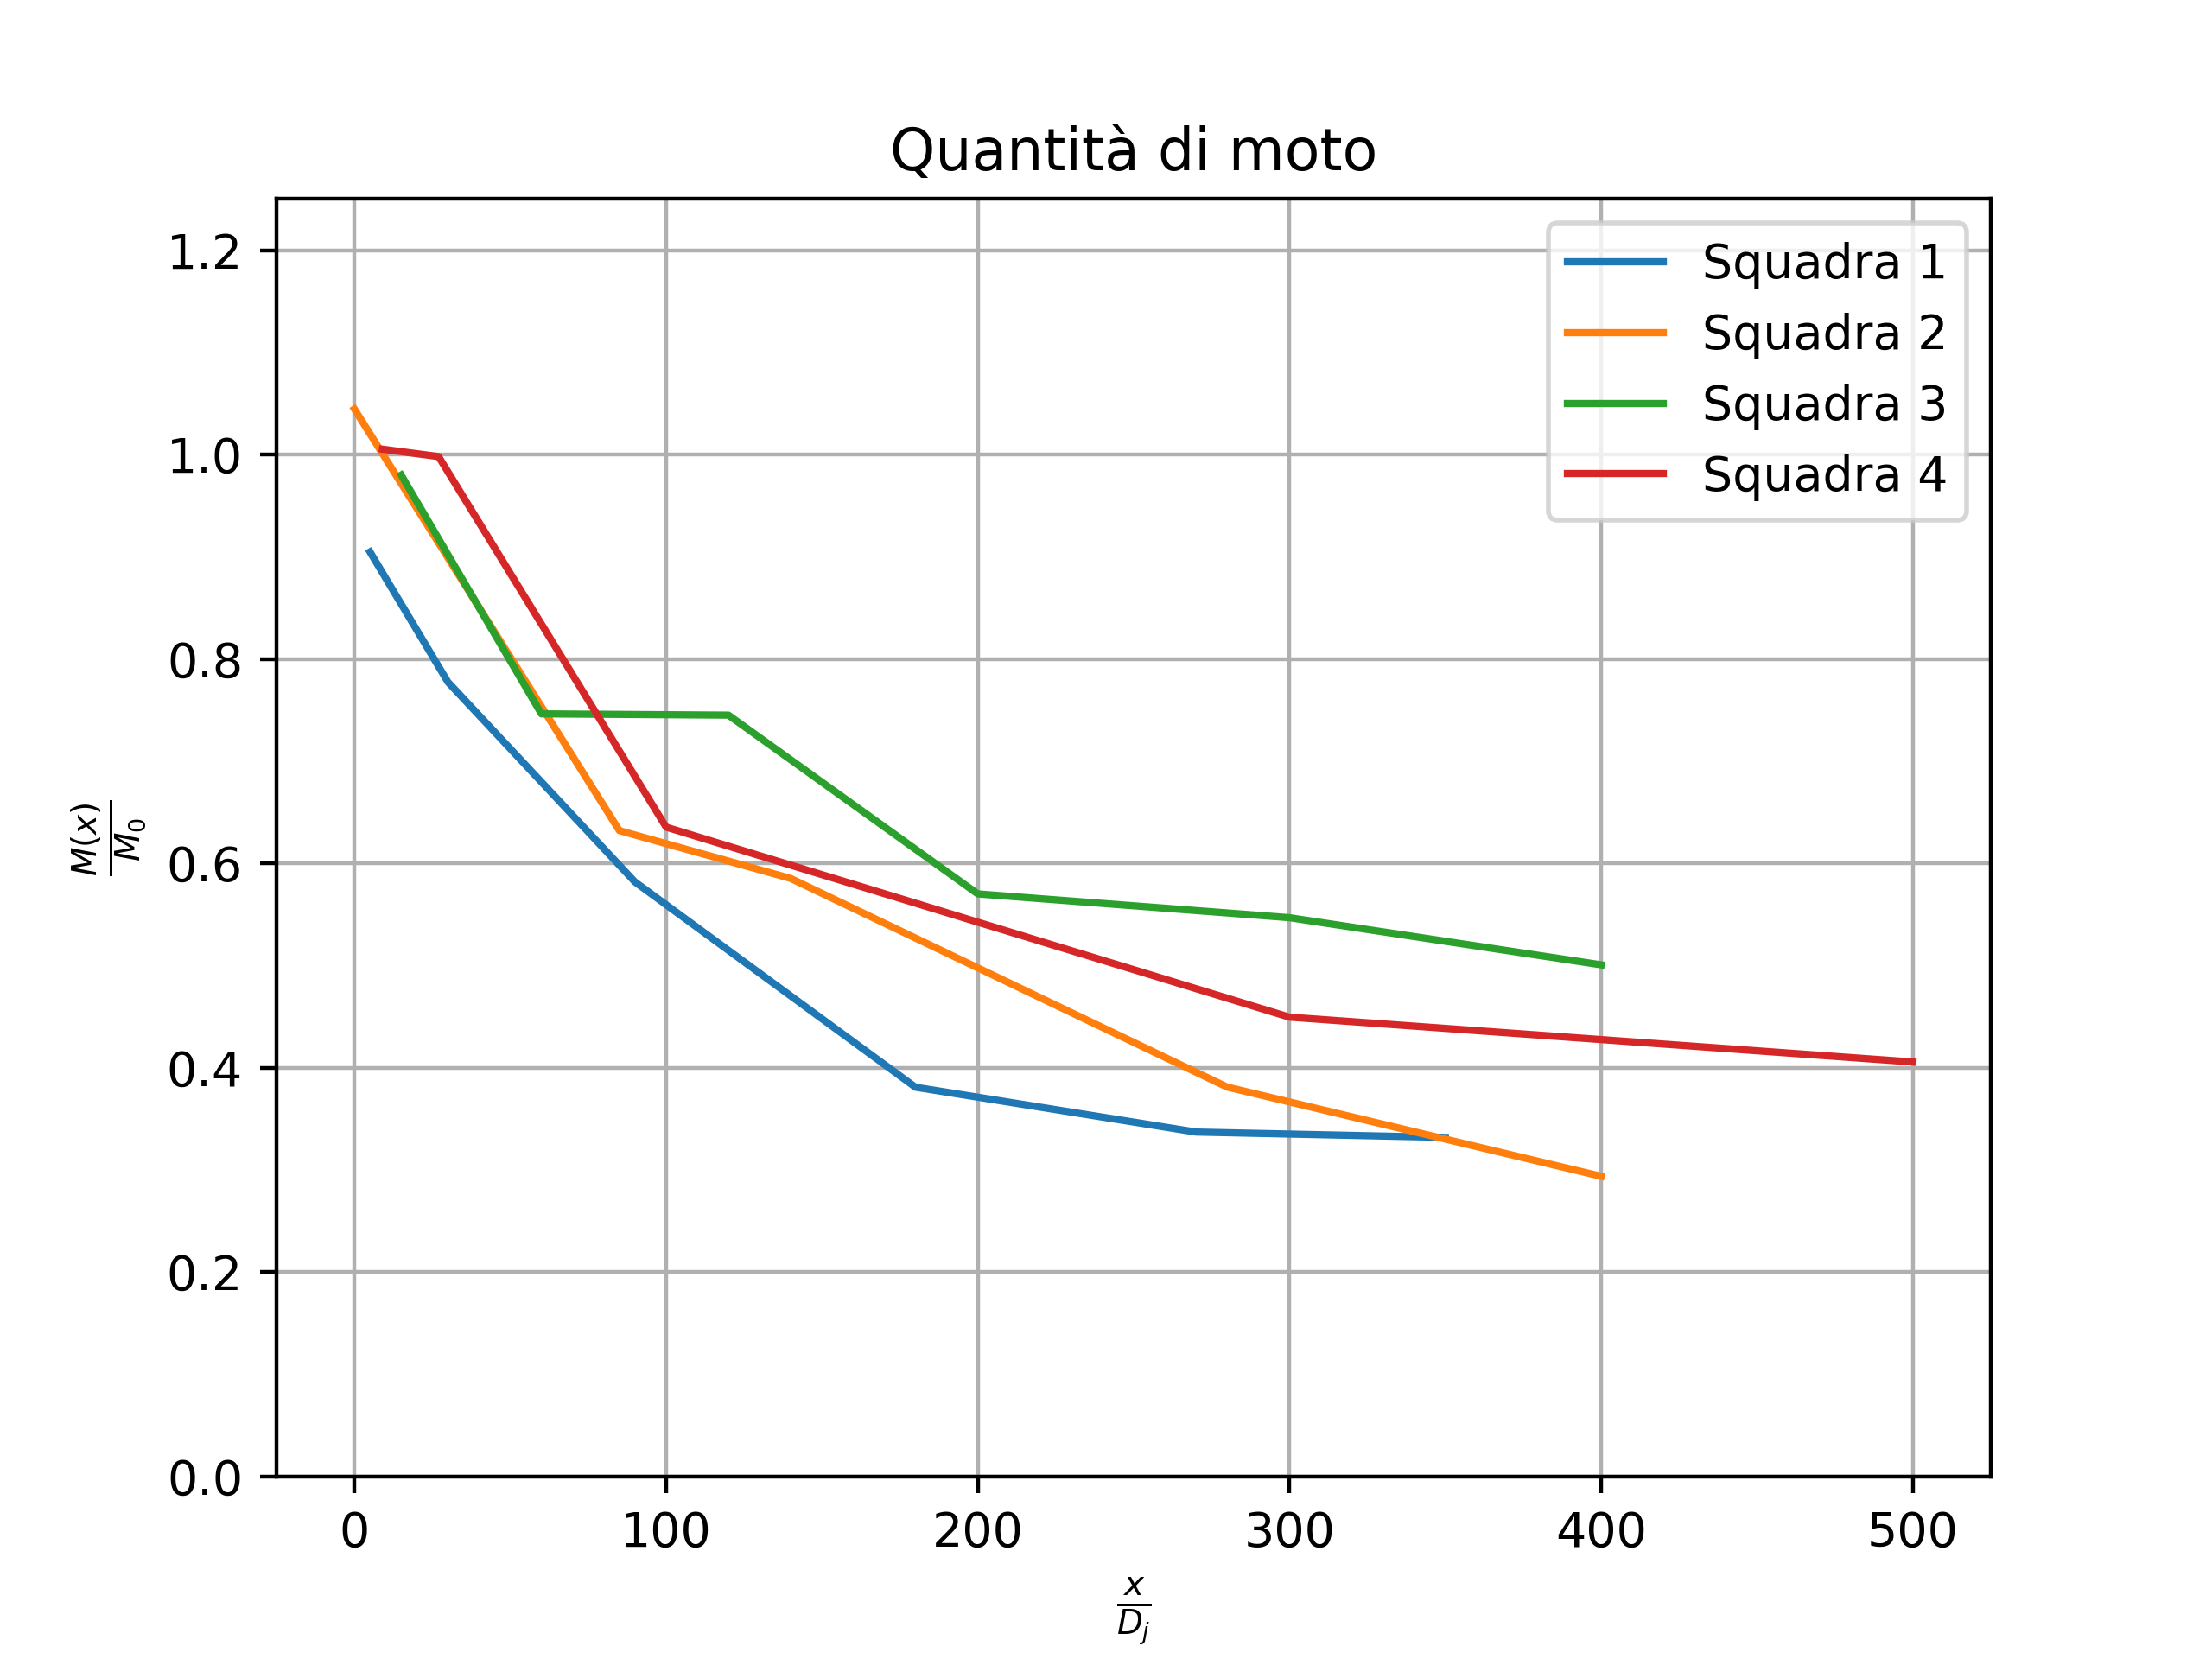
\includegraphics[width=.7\linewidth]{images/4/qdm.png}
    \caption{Quantità di moto}
\end{figure}

\noindent L'andamento decrescente è dovuto al fatto che i dati raccolti non hanno coperto una distanza radiale $r$ infinita, pertanto parte della quantità di moto non è rilevata.

\subsection{Energia}
A causa della dissipazione viscosa, l'energia si prospetta decrescente lungo l'asse del getto.\\\\
Per scrivere l'energia nell'unità di tempo che compete ad ogni sezione basta scrivere l'energia cinetica elementare del moto medio e riferirla all'unità di tempo:
\begin{equation*}
    E = \frac{dE_c}{dt} = \frac12 \frac{dm}{dt} u^2 = \frac12 G u^2 = \frac12 2\pi\rho \int_0^\infty u^3r dr
\end{equation*}
Quindi:
\begin{equation*}
    E = \pi\rho \int_0^\infty u^3r dr \quad \left[W\right]
\end{equation*}
L'energia in corrispondenza della sezione di uscita è invece:
\begin{equation*}
    E_0 = \frac12 \rho \left( \frac{\pi D^2}4 \right) U_0^3
\end{equation*}
Valutando la funzione integranda in modo discreto utilizzando i dati sperimentali, è possibile risolvere l'integrale con l'applicazione della regola dei trapezi.\\\\
Diagrammando l'andamento dell'energia $E$ normalizzata rispetto al valore in corrispondenza della sezione di uscita $E_0$ si ottiene il seguente diagramma:
\begin{figure}[h]
    \centering
    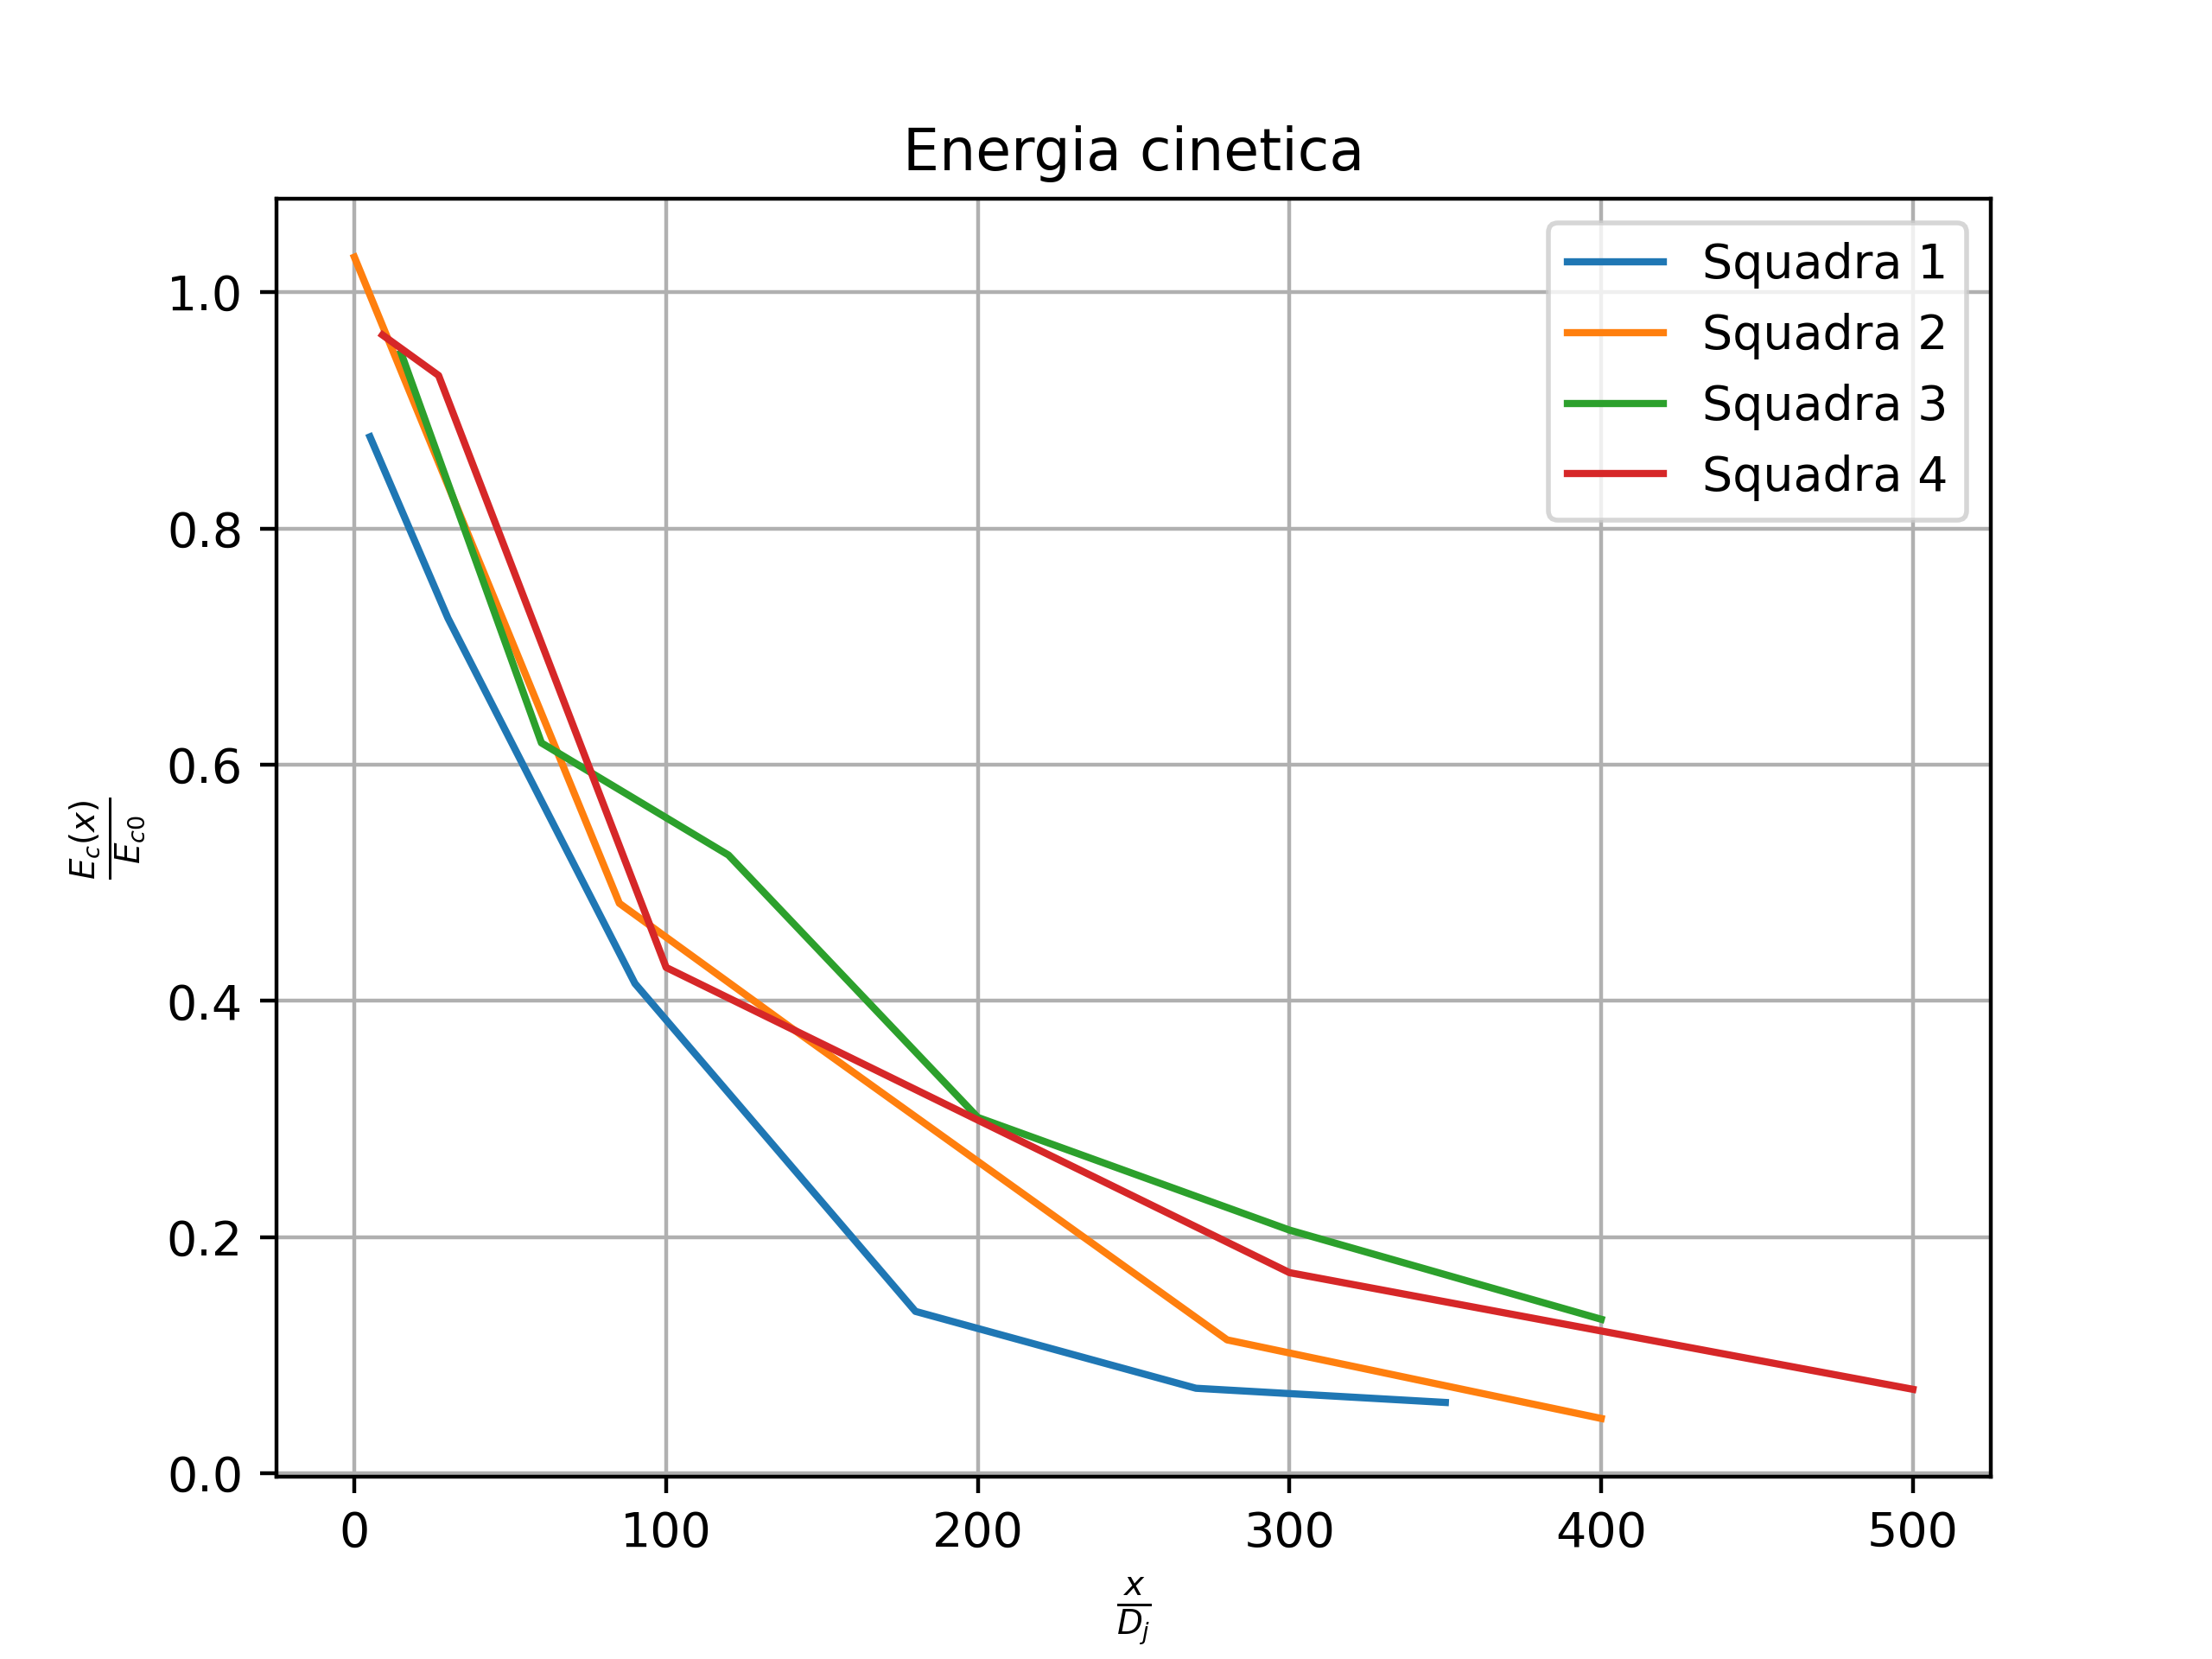
\includegraphics[width=.8\linewidth]{images/4/energia.png}
    \caption{Energia}
\end{figure}
\section{Profilo alare NACA 0015}
Nel presente esperimento sono valutate le caratteristiche aerodinamiche del profilo alare NACA 0015 mediante la misura della distribuzione di pressione al variare dell'incidenza e del numero di Reynolds. Sono inoltre determinate le curve del coefficiente di portanza $C_L(\alpha)$ e del coefficiente di momento aerodinamico $C_M(\alpha)$ rispetto all'incidenza $\alpha$ e la posizione del centro di pressione e del fuoco del profilo alare.
\begin{figure}[H]
    \centering
    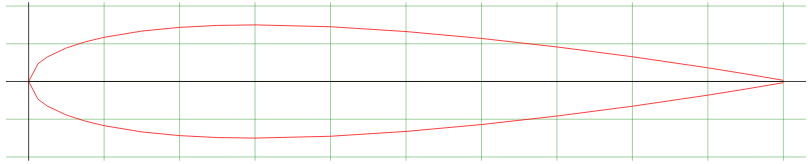
\includegraphics[width=\textwidth]{images/5/naca0015airfoiltools.png}
    \caption{Profilo alare NACA 0015}
\end{figure}

\subsection{Geometria del profilo alare}
I profili alari NACA sono forme geometriche standardizzate sviluppate dal National Advisory Committee for Aeronautics (NACA) degli Stati Uniti d'America. Un profilo alare NACA è definito da un numero, solitamente di quattro o cinque cifre, che ne determina le caratteristiche. In particolare, nei profili alari Naca a quattro cifre:
\begin{itemize}
    \item La prima cifra indica la curvatura massima come percentuale della corda;
    \item La seconda cifra fornisce la distanza del punto di massima curvatura dal bordo d'attacco espressa come percentuale della corda e in multipli di dieci;
    \item Le ultime due cifre descrivono il massimo spessore del profilo alare espresso come percentuale della corda.
\end{itemize}
Ad esempio, il profilo alare NACA 2412 presenta una curvatura massima del 2\%, situata al 40\% della corda partendo dal bordo d'attacco e ha uno spessore massimo del 12\% della corda. Nei profili alari NACA a quattro cifre lo spessore massimo è sempre posizionaot al 30\% della corda, sempre partendo dal bordo d'attacco.\\\\
Il profilo alare NACA 0015, preso in esame, è simmetrico, in quanto le cifre 00 indicano che non vi è una curvatura. Il 15 indica che lo spessore massimo è il 15\% della sua lunghezza.
\newpage
\noindent La formula per generare la forma di un profio alare NACA $00xx$, dove "$xx$" va sostituito con lo spessore massimo espresso come percentuale della corda, è:
\begin{equation*}
    y_t = 5tc\left[ 0.2969\sqrt{\frac{x}{c}} -0.1260\left(\frac{x}{c}\right) -0.3516\left(\frac xc \right)^2 + 0.2843 \left( \frac xc \right)^3 -0.1015 \left( \frac xc \right)^4 \right]
\end{equation*}
Dove:
\begin{itemize}
    \item $c$ è la lunghezza della corda;
    \item $x$ è la posizione lungo la corda da 0 a $c$;
    \item $y_t$ è metà dello spessore ad un dato valore di $x$;
    \item $t$ è lo spessore massimo espresso come frazione della corda, in modo che $100\,t$ sia uguale alle ultime due cifre del codice NACA.
\end{itemize}

\subsection{Descrizione dell'esperimento}
Nella presente attività, il profilo alare NACA 0015, di corda pari a $c=100$ mm, è studiato con l'utilizzo di una galleria del vento. Le forze di pressione esercitate dal fluido sul profilo giaccino sul piano del campo di moto. Le forza aerodinamica generata dal flusso può essere scomposta in due componenti, una parallela ed una normale alla velocità, rispettivamente la resistenza e la portanza. Tali forze risultano applicate in un punto detto centro di pressione.\\\\
Nota la distribuzione di pressione relativa $p-p_\infty$ sulla superficie del profilo $S$, la risultante delle forze aerodinamiche $F$ è data da:
\begin{equation*}
    F = \int_S (p-p_\infty)\vec n dS
\end{equation*}
Considerando un profilo immerso in una corrente uniforme di velocità $V_\infty$, posto ad incidenza $\alpha$, si utilizzano i pedici $+$ e $-$ per indicare le grandezze riferite rispettivamente a dorso e ventre del profilo.\\\\
Considerando un tratto di superficie del dorso di profondità unitaria, si ha:
\begin{equation*}
    dF_+ = (p_+ - p_\infty)(ds_+ \cdot 1)
\end{equation*}
La sua scomposizione lungo le coordinate $x$ e $y$, indicando con $\gamma$ l'angolo che rappresenta la pendenza locale della superficie del profilo, è:
\begin{equation*}
    dF_+|_x = (p_+ - p_\infty)(ds_+)\sin \gamma \quad dF_+|_y = (p_+ - p_\infty)(ds_+)\cos \gamma
\end{equation*}
Analogamente per il ventre:
\begin{equation*}
    dF_-|_x = (p_- - p_\infty)(ds_-)\sin \gamma \quad dF_-|_y = (p_- - p_\infty)(ds_-)\cos \gamma
\end{equation*}
Integrando tali forze elementari, si ricavano le componenti $R_x$ ed $R_y$ della forza aerodinamica risultante $F$:
\begin{equation*}
    R_x = \int_0^c (dF_+|_x + dF_-|_x)dx
\end{equation*}
\begin{equation*}
    R_y = \int_0^c (dF_+|_y + dF_-|_y)dy
\end{equation*}
Dalle due componenti si ricavano la portanza $L$ e la resistenza $D$ che risultano essere le componenti della forza aerodinamica proiettate rispettivamente perpendicolarmente e parallelamente alla velocità $V_\infty$ a monte del profilo:
\begin{equation*}
    L = R_y \cos \alpha + R_x \sin \alpha
\end{equation*}
\begin{equation*}
    D = R_x \cos \alpha + R_y \sin \alpha
\end{equation*}
Per piccoli angoli di incidenza, si può approssimare:
\begin{equation*}
    L\approx R_y = \int_0^c \left[ (p_--p_\infty) - (p_+-p_\infty) \right] dx
\end{equation*}
Definendo il coefficiente di pressione:
\begin{equation*}
    c_p = \frac{p-p_\infty}{\frac12 \rho V_\infty^2}
\end{equation*}
Si può riscrivere l'espressione della portanza come:
\begin{equation*}
    L = \frac12 \rho V^2_\infty \int_0^c (c_{p-}-c_{p+})dx
\end{equation*}
Introducendo il coefficiente portanza, e considerando un flusso bidimensionale, si può adimensionalizzare la portanza rispetto ad una superficie di larghezza pari alla corda $c$ e profondità unitaria:
\begin{equation*}
    c_L = \int_0^1(c_{p-}-c_{p+})d\left( \frac xc \right)
\end{equation*}
Il coefficiente di portanza è quindi valutato come l'area sottesa tra le curve $c_{p-}$ e $c_{p+}$.\\\\
Ulteriore obiettivo dell'attività consiste nel calcolo del coefficiente di momento $c_M$. Per comodità si sposta il punto di applicazione della portanza al bordo di attacco (leading edge) del profilo. Si assume per convenzione un momento positivo cabrante. Il momento elementare agente sull'elemento di superficie di profondità unitaria $ds$, trascurando il contributo dovuto al braccio lungo la direzione $y$, vale:
\begin{equation*}
    dM_{LE} = (dF_+|_y - dF_-|_y) x
\end{equation*}
Integrando si ottiene l'espressione per il momento al bordo di attacco:
\begin{equation*}
    M_{LE} = -\int_0^c \left[ (p_- - p_\infty)- (p_+ - p_\infty) \right] xdx
\end{equation*}
Con considerazioni analoghe alle precedenti si passa in termini adimensionali introducendo il coefficiente di momento:
\begin{equation*}
    c_{M_{LE}} = \frac{M_{LE}}{\frac12 \rho V_\infty^2 c^2} = -\int_0^1 (c_{p-}-c_{p+}) \left( \frac xc \right) d\left( \frac xc \right)
\end{equation*}
A questo punto, si può ricavare il centro di pressione $x_{cp}$. Conoscendo il momento al bordo di attacco e la portanza, si ha:
\begin{equation*}
    M_{LE} = -x_{cp} L
\end{equation*}
Che in termini adimensionali si traduce in:
\begin{equation*}
    c_{M_{LE}} = - \frac{x_{cp}}c c_L
\end{equation*}
Si ottiene quindi la relazione per la posizione del centro di pressione, che sarà funzione dell'incidenza:
\begin{equation*}
    \frac{x_{cp}}c = -\frac{c_{M_{LE}}}{c_L} = f(\alpha)
\end{equation*}
Dal coefficiente di portanza e dal coefficiente di momento al bordo di attacco è possibile stimare la posizione del fuoco, o centro aerodinamico $x_{ac}$, del profilo. Nel centro aerodinamico vale la proprietà focale: il momento aerodinamico rimane costante al variare dell'incidenza.\\\\
Il momento aerodinamico nel fuoco del profilo può essere scritto come:
\begin{equation*}
    M_{ac} = - L (x_{cp}-x{ac}) = -(Lx_{xp}) + Lx_{ac} = M_{LE} + Lx_{ac}
\end{equation*}
Tale relazione, in termini adimensionali, si traduce in:
\begin{equation*}
    c_{M_{ac}} = c_{M_{LE}} + c_L \frac{x_{ac}}c
\end{equation*}
Per il calcolo della posizione del fuoco è sufficiente quindi imporre la condizione focale:
\begin{equation*}
    \frac{\partial c_{M_{ac}}}{\partial \alpha} = 0
\end{equation*}
Avendo cura di sostituire l'espressione per il coefficiente di momento sul bordo di attacco e per il coefficiente di portanza nel tratto lineare delle rispettive curve.\\\\
Per un profilo in campo subsonico, la posizione del centro aerodinamico corrisponde a circa il 25\% della corda, mentre nel caso di campo supersonico il fuoco dei profili alare è posizionato in corrispondenza del 50\% della corda.\\\\
Una volta calcolato il fuoco del profilo è infine possibile ricavare il coefficiente di momento aerodinamico:
\begin{equation*}
    c_{M_{ac}} = c_{M_{LE}} + c_L \frac{x_{ac}}c
\end{equation*}
Per la proprietà focale, questo deve mantenersi costante al variare dell'incidenza.

\subsection{Catena di misura}
Per misurare la distribuzione di pressione sul dorso e sul ventre del profilo alare, questo è studiato in una galleria del vento aperta.
\begin{figure}[H]
    \centering
    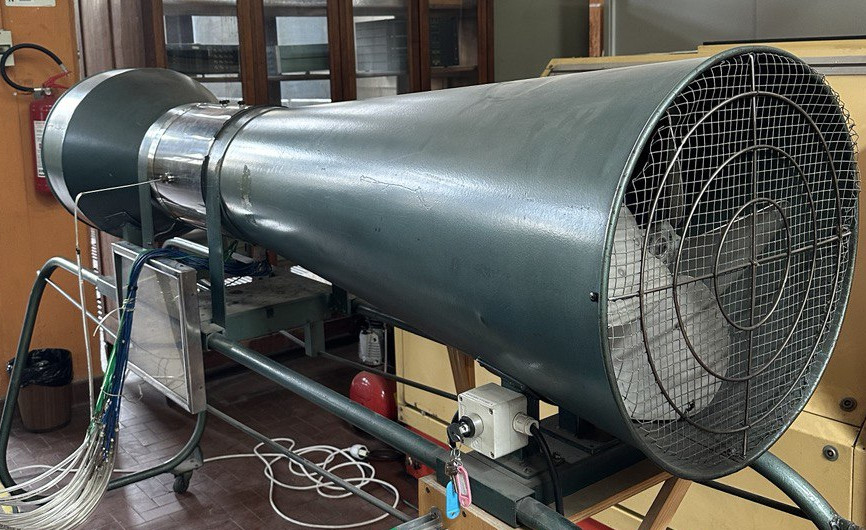
\includegraphics[width=.7\textwidth]{images/5/galleria.jpg}
    \caption{Galleria del vento}
\end{figure}

\noindent Per allineare il flusso e ridurre la turbolenza, all'entrata del convergente della galleria è presente un honeycomb.
\begin{figure}[H]
    \centering
    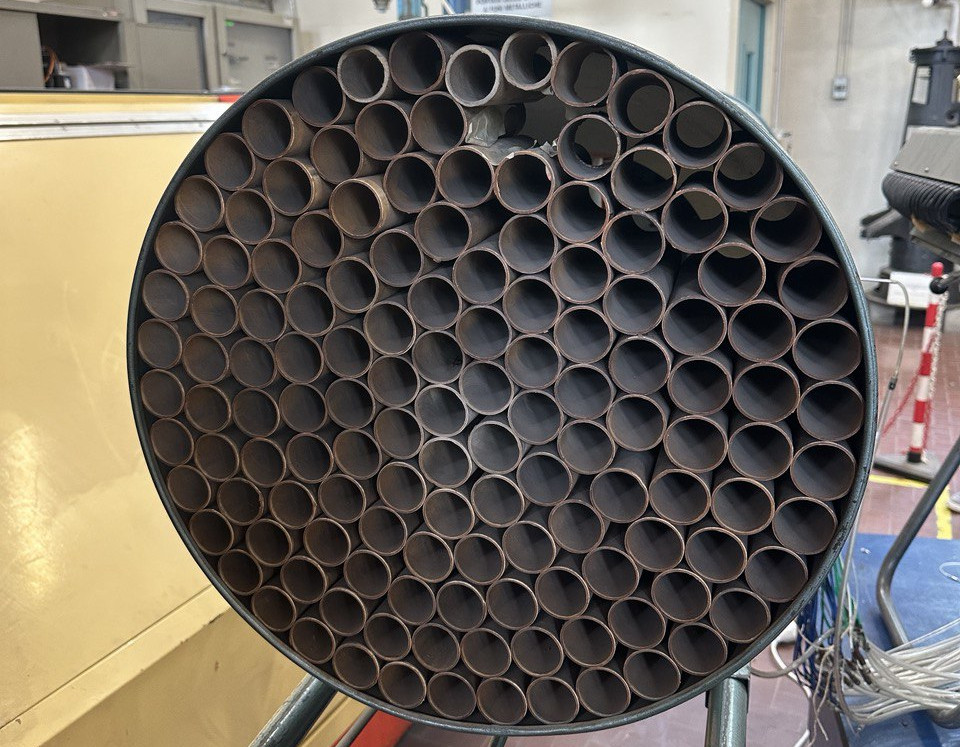
\includegraphics[width=.6\textwidth]{images/5/honeycomb.jpg}
    \caption{Honeycomb}
\end{figure}

\noindent Sul profilo alare sono posizionate 11 prese di pressione, alle seguenti coordinate dal bordo di attacco:
\begin{equation*}
    \left( \frac xc \right) = 0,\ 2.5,\ 5,\ 10,\ 20,\ 30,\ 40,\ 50,\ 60,\ 70,\ 80
\end{equation*}
Queste prese sono presenti solo su una faccia del profilo, questo perché data la geometria simmetrica, il campo di pressione rilevato sul dorso ad un angolo di incidenza positiva è uguale al campo di pressione che si rileva sul ventre allo stesso angolo di incidenza con segno opposto.
\begin{figure}[h]
    \centering
    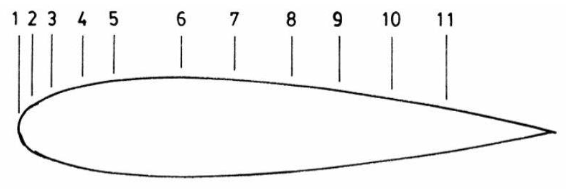
\includegraphics[width=.8\textwidth]{images/5/posizioneprese.png}
    \caption{Posizione delle prese statiche di pressione sul profilo alare}
\end{figure}

\noindent La misurazione della pressione statica localmente sul profilo è basata su una considerazione fondamentale, osservando le equazioni di Navier-Stokes specializzate per lo strato limite bidimensionale.
\begin{equation*}
    \begin{dcases}
        &\frac{\partial u}{\partial x} + \frac{\partial v}{\partial y} = 0\\
        & u\frac{\partial u}{\partial x} + v\frac{\partial u}{\partial y} = -\frac1\rho \frac{\partial P}{\partial x} + \nu\left( \frac{\partial^2 u}{\partial x^2} + \frac{\partial^2 u}{\partial y^2} \right)\\
        & u\frac{\partial v}{\partial x} + v\frac{\partial v}{\partial y} = -\frac1\rho \frac{\partial P}{\partial y} + \nu\left( \frac{\partial^2 v}{\partial x^2} + \frac{\partial^2 v}{\partial y^2} \right)
    \end{dcases}
\end{equation*}
Tenuto conto che nello strato limite tutte le grandezze variano rapidamente con l'ordinata $y$ e lentamente con l'ascissa $x$ e che è sempre verificata la condizione di piccole perturbazioni, la terza equazione si riduce a:
\begin{equation*}
    \frac{\partial P}{\partial y} = 0
\end{equation*}
Cioè la pressione statica nello strato limite lungo la coordinata $y$ rimane costante. Grazie a questa considerazione è possibile considerare la pressione statica misurata a parete uguale alla pressione statica appena fuori dallo strato limite, ottenendo quindi informazioni sul campo di moto attorno al profilo.\\\\
Oltre alle 11 prese di pressione statica sul profilo, sono presenti altre due prese subito a valle del convergente, una per la pressione totale ed una per la pressione statica. Queste 13 prese sono collegate tramite condotti pneumatici ad un multimanometro differenziale.\\\\
In particolare, la presa di pressione statica all'ingresso della camera di prova e la presa di pressione totale della corrente sono connesse con le canne 1 e 2 del multimanometro, le canne 3 e 4 sono libere e quindi rilevano la pressione ambiente mentre le altre 11 canne sono impegnate dai segnali delle prese su una delle due facce del profilo alare.
\begin{figure}[H]
    \centering
    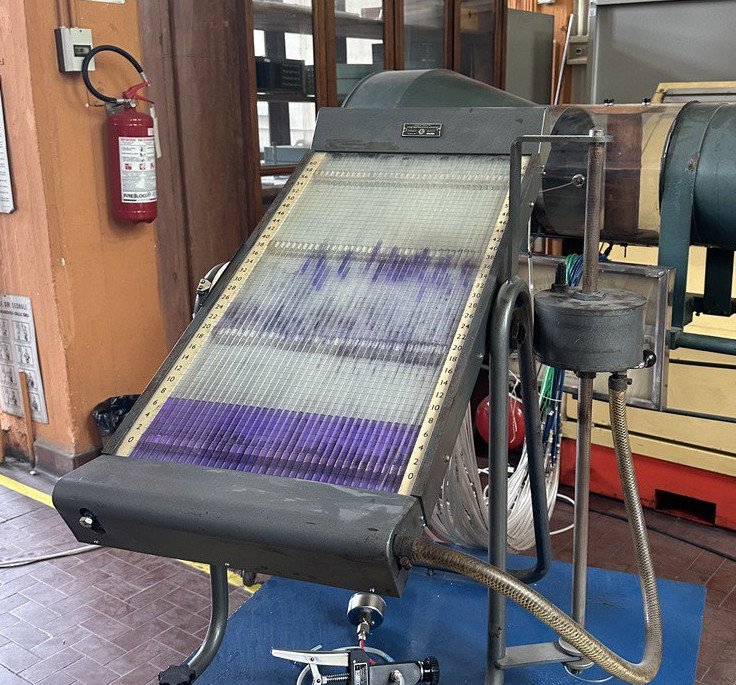
\includegraphics[width=.8\textwidth]{images/5/multimanometro.jpg}
    \caption{Multimanometro}
\end{figure}

\noindent Le canne manometriche sono inclinate con un angolo $\beta=15^\circ$ e riempite con alcool etilico, di densità nota $\rho_{fm} = 0.789$ g/cm$^3$.\\\\
Il peso specifico del fluido manometrico si ottiene come:
\begin{equation*}
    \gamma_{fm} = g_0 \rho_{fm} = 7732\ \text{N/m}^3
\end{equation*}
Inoltre, a partire dai valori di pressione e temperatura ambiente, si ricava la densità dell'aria dalla legge dei gas perfetti e la viscosità dinamica dalla legge di Sutherland:
\begin{equation*}
    \rho = \frac{p_{amb}}{RT_{amb}} \qquad \mu = 1.46\cdot10^{-6} \frac{T_{amb}^{3/2}}{T_{amb}+110}
\end{equation*}
Dalla legge di Stevino, misurando le altezze delle canne manometriche con l'apposita scala graduata in centimetri, si ricavano i valori di pressione:
\begin{equation*}
    (p-p_{ref}) = (h_{ref}-h) \gamma_{fm} \sin \beta
\end{equation*}
Dalla relazione di Bernoulli, si ottiene il valore della velocità indisturbata a monte:
\begin{equation*}
    V_\infty = \sqrt{\frac{2q}\rho} = \sqrt{\frac{2(p_{0\infty}-p_\infty)}{\rho}}
\end{equation*}
Pertanto si può valutare il coefficiente di pressione come:
\begin{equation*}
    c_p = \frac{p-p_{\infty}}{\frac12 \rho V_\infty^2} = \frac{p-p_\infty}{p_{0\infty}-p_\infty} = \frac{h_\infty-h}{h_\infty-h_{0\infty}}
\end{equation*}

\subsection{Procedura sperimentale}
L'esperimento è condotto variando l'angolo d'incidenza del profilo alare ruotandolo sul cinematismo e controllando i gradi di rotazione con un goniometro.\\\\
Ogni squadra ha utilizzato un diverso valore di portata, quindi un diverso numero di Reynolds, costante per tutte le incidenze esaminate.\\\\
Per ogni angolo di incidenza, si avvia la galleria, si attende il termine di eventuali fenomeni transitori e una volta che le canne manometriche si stabilizzano si registrano i rispettivi valori con una fotografia.\\\\
Si prendono prima tutti i dati ad angoli di incidenza positivi, rappresentativi dei profili di pressione sul dorso, poi si prendono le misure utilizzando gli stessi angoli di incidenza ma di segno negativo, rappresentativi dei profili di pressione sul ventre del profilo.\\\\
I dati grezzi ottenuti sono quindi manualmente riportati in una tabella ad esempio in Microsoft Excel. Le tabelle di dati grezzi ottenute per le quattro squadre per la presente attività sono riportate in appendice \ref{a5}.\\\\
Si riportano a seguire alcuni istogrammi rappresentativi delle colonne di fluido manometrico:
\begin{figure}[H]
    \centering
    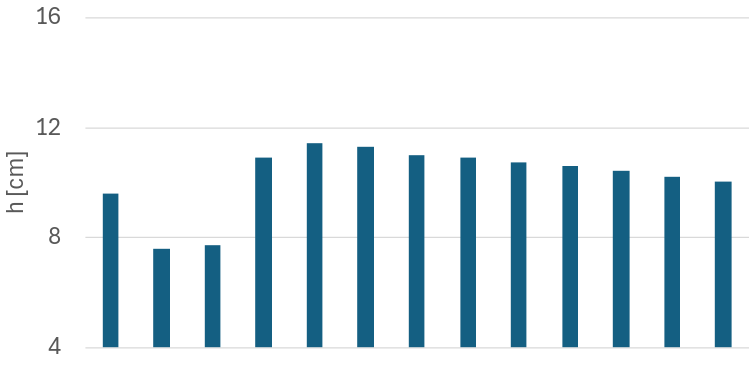
\includegraphics[width=.49\textwidth]{images/5/dsq1a0.png}
    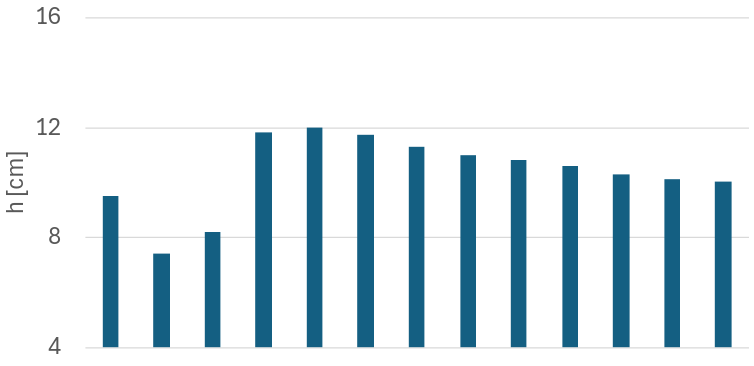
\includegraphics[width=.49\textwidth]{images/5/dsq1a2.png}
    \caption{Istogrammi per la squadra 1 ad incidenza 0 e 2 gradi}
\end{figure}

\begin{figure}[H]
    \centering
    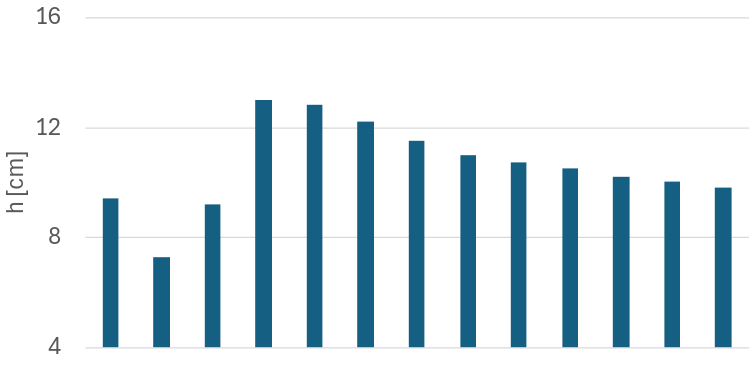
\includegraphics[width=.49\textwidth]{images/5/dsq1a4.png}
    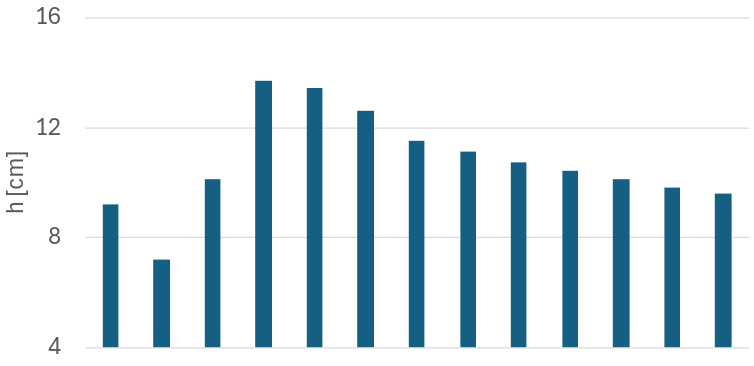
\includegraphics[width=.49\textwidth]{images/5/dsq1a6.png}
    \caption{Istogrammi per la squadra 1 ad incidenza 4 e 6 gradi}
\end{figure}

\begin{figure}[H]
    \centering
    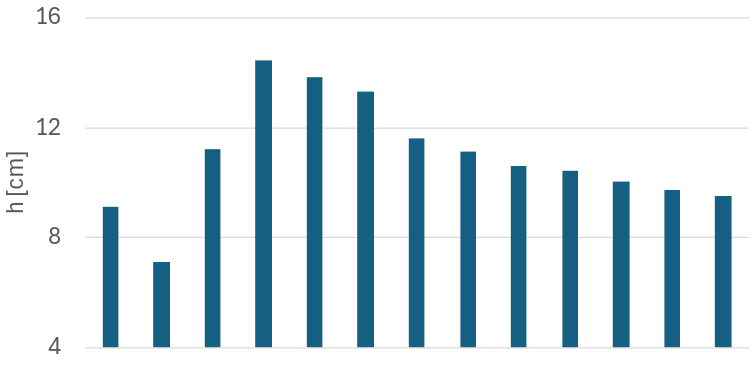
\includegraphics[width=.49\textwidth]{images/5/dsq1a8.png}
    \includegraphics[width=.49\textwidth]{images/5/dsq1a10.png}
    \caption{Istogrammi per la squadra 1 ad incidenza 8 e 10 gradi}
\end{figure}

\begin{figure}[H]
    \centering
    \includegraphics[width=.49\textwidth]{images/5/dsq1a0.png}
    \includegraphics[width=.49\textwidth]{images/5/dsq1a-2.png}
    \caption{Istogrammi per la squadra 1 ad incidenza 0 e -2 gradi}
\end{figure}

\begin{figure}[H]
    \centering
    \includegraphics[width=.49\textwidth]{images/5/dsq1a-4.png}
    \includegraphics[width=.49\textwidth]{images/5/dsq1a-6.png}
    \caption{Istogrammi per la squadra 1 ad incidenza -4 e -6 gradi}
\end{figure}

\begin{figure}[H]
    \centering
    \includegraphics[width=.49\textwidth]{images/5/dsq1a-8.png}
    \includegraphics[width=.49\textwidth]{images/5/dsq1a-10.png}
    \caption{Istogrammi per la squadra 1 ad incidenza -8 e -10 gradi}
\end{figure}

\begin{figure}[H]
    \centering
    \includegraphics[width=.49\textwidth]{images/5/dsq1a14.png}
    \includegraphics[width=.49\textwidth]{images/5/dsq1a-14.png}
    \caption{Istogrammi per la squadra 1 ad incidenza 14 e -14 gradi}
\end{figure}

\begin{figure}[H]
    \centering
    \includegraphics[width=.49\textwidth]{images/5/dsq2a0.png}
    \includegraphics[width=.49\textwidth]{images/5/dsq2a2.png}
    \caption{Istogrammi per la squadra 2 ad incidenza 0 e 2 gradi}
\end{figure}

\begin{figure}[H]
    \centering
    \includegraphics[width=.49\textwidth]{images/5/dsq2a4.png}
    \includegraphics[width=.49\textwidth]{images/5/dsq2a6.png}
    \caption{Istogrammi per la squadra 2 ad incidenza 4 e 6 gradi}
\end{figure}

\begin{figure}[H]
    \centering
    \includegraphics[width=.49\textwidth]{images/5/dsq2a8.png}
    \includegraphics[width=.49\textwidth]{images/5/dsq2a10.png}
    \caption{Istogrammi per la squadra 2 ad incidenza 8 e 10 gradi}
\end{figure}

\begin{figure}[H]
    \centering
    \includegraphics[width=.49\textwidth]{images/5/dsq2a0.png}
    \includegraphics[width=.49\textwidth]{images/5/dsq2a-2.png}
    \caption{Istogrammi per la squadra 2 ad incidenza 0 e -2 gradi}
\end{figure}

\begin{figure}[H]
    \centering
    \includegraphics[width=.49\textwidth]{images/5/dsq2a-4.png}
    \includegraphics[width=.49\textwidth]{images/5/dsq2a-6.png}
    \caption{Istogrammi per la squadra 2 ad incidenza -4 e -6 gradi}
\end{figure}

\begin{figure}[H]
    \centering
    \includegraphics[width=.49\textwidth]{images/5/dsq2a-8.png}
    \includegraphics[width=.49\textwidth]{images/5/dsq2a-10.png}
    \caption{Istogrammi per la squadra 2 ad incidenza -8 e -10 gradi}
\end{figure}

\subsection{Analisi dati}
L'analisi dati per la presente attività è condotta con l'ausilio di un codice Python, riportato in appendice \ref{b5}.\\\\
Come prima operazione si calcola la densità e la viscosità dinamica, a partire dalla pressione e dalla temperatura ambiente, utilizzando la legge dei gas perfetti e la legge di Sutherland:
\begin{equation*}
    \rho = \frac{p_{amb}}{RT_{amb}} \qquad \mu = 1.46\cdot10^{-6} \frac{T_{amb}^{3/2}}{T_{amb}+110}
\end{equation*}
Poi, dalla relazione di Bernoulli, si ricava la velocità a monte per ogni misura:
\begin{equation*}
    V_\infty = \sqrt{\frac{2(h_{\infty}-h) \gamma_{fm} \sin \beta}{\rho}}
\end{equation*}
Quindi a seguire il numero di Reynolds:
\begin{equation*}
    Re = \frac{\rho V_\infty c}{\mu}
\end{equation*}
Si ottengono i seguenti numeri di Reynolds per le quattro squadre:
\begin{equation*}
    Re = 75000,\ 100000,\ 90000,\ 120000
\end{equation*}

\subsubsection{Coefficiente di pressione}
Dai dati sulle altezze delle canne manometriche è immediato ricavare i coefficienti di pressioni valutati ad ogni posizione sul profilo e per ogni incidenza:
\begin{equation*}
    c_p(x,\alpha) = \frac{h_\infty-h}{h_\infty - h_{0\infty}}
\end{equation*}
Per effettuare i seguenti calcoli è stata utilizzato un foglio di calcolo in Microsoft Excel. Dal valore del coefficiente di pressione è inoltre possibile ricavare i profili di velocità:
\begin{equation*}
    \frac{V(x,\alpha)}{V_\infty} = \sqrt{1-c_p}
\end{equation*}
Poiché, per motivi strutturali, non sono presenti prese di pressione statiche fino al bordo di fuga del profilo, bensì solo fino all'80\% della corda, è opportuno valutare il valore di coefficiente di pressione sul bordo di fuga interpolando i dati delle prese di pressione statica precedenti, con l'accortezza di rispettare la condizione di Kutta, tale per cui sul bordo di fuga:
\begin{equation*}
    p_+ = p_-
\end{equation*}
Utilizzando i coefficienti di pressione calcolati ed i coefficienti di pressione al bordo di attacco estrapolati, si ottengono i diagrammi riportati a seguire.
\begin{figure}[H]
    \centering
    \includegraphics[width=.49\textwidth]{images/5/cp1 a=0.png}
    \includegraphics[width=.49\textwidth]{images/5/cp1 a=2.png}
    \includegraphics[width=.49\textwidth]{images/5/cp1 a=4.png}
    \includegraphics[width=.49\textwidth]{images/5/cp1 a=6.png}
    \includegraphics[width=.49\textwidth]{images/5/cp1 a=8.png}
    \includegraphics[width=.49\textwidth]{images/5/cp1 a=10.png}
    \includegraphics[width=.49\textwidth]{images/5/cp1 a=14.png}
    \includegraphics[width=.49\textwidth]{images/5/cp1.png}
\end{figure}
\begin{figure}[H]
    \centering
    \includegraphics[width=.49\textwidth]{images/5/cp2 a=0.png}
    \includegraphics[width=.49\textwidth]{images/5/cp2 a=2.png}
    \includegraphics[width=.49\textwidth]{images/5/cp2 a=4.png}
    \includegraphics[width=.49\textwidth]{images/5/cp2 a=6.png}
    \includegraphics[width=.49\textwidth]{images/5/cp2 a=8.png}
    \includegraphics[width=.49\textwidth]{images/5/cp2 a=10.png}
    \includegraphics[width=.49\textwidth]{images/5/cp2 a=15.png}
    \includegraphics[width=.49\textwidth]{images/5/cp2.png}
\end{figure}
\begin{figure}[H]
    \centering
    \includegraphics[width=.49\textwidth]{images/5/cp3 a=0.png}
    \includegraphics[width=.49\textwidth]{images/5/cp3 a=2.png}
    \includegraphics[width=.49\textwidth]{images/5/cp3 a=4.png}
    \includegraphics[width=.49\textwidth]{images/5/cp3 a=6.png}
    \includegraphics[width=.49\textwidth]{images/5/cp3 a=8.png}
    \includegraphics[width=.49\textwidth]{images/5/cp3 a=10.png}
    \includegraphics[width=.49\textwidth]{images/5/cp3 a=14.png}
    \includegraphics[width=.49\textwidth]{images/5/cp3.png}
\end{figure}
\begin{figure}[H]
    \centering
    \includegraphics[width=.49\textwidth]{images/5/cp4 a=0.png}
    \includegraphics[width=.49\textwidth]{images/5/cp4 a=2.png}
    \includegraphics[width=.49\textwidth]{images/5/cp4 a=4.png}
    \includegraphics[width=.49\textwidth]{images/5/cp4 a=6.png}
    \includegraphics[width=.49\textwidth]{images/5/cp4 a=10.png}
    \includegraphics[width=.49\textwidth]{images/5/cp4 a=12.png}
    \includegraphics[width=.49\textwidth]{images/5/cp4 a=15.png}
    \includegraphics[width=.49\textwidth]{images/5/cp4.png}
\end{figure}

\noindent Si nota come, alla presa di pressione statica posizionata sul bordo di attacco del profilo, si hanno due valori di coefficiente di pressione diversi tra dorso e ventre. Questo non è possibile fisicamente, si attribuisce tale discrepanza all'accuratezza della misura dell'angolo di incidenza sul goniometro nella camera di prova oppure ad un posizionamento della presa di pressione statica non perfettamente coincidente con il bordo di attacco del profilo.\\\\
Risulta inoltre evidente dall'andamento del coefficiente di pressione sul dorso come ad elevate incidenze ($\alpha > 12^\circ$) si verifichi lo stallo, infatti l'area sottesa tra le due curve, rappresentativa della portanza, si riduce drasticamente.\\\\
Questo era in realtà già evidente dalla visualizzazione delle canne manometriche:
\begin{figure}[H]
    \centering
    \includegraphics[width=.49\textwidth]{images/5/dsq1a10.png}
    \includegraphics[width=.49\textwidth]{images/5/dsq1a14.png}
    \caption{Istogrammi per la squadra 1 ad incidenza 10 e 14 gradi}
\end{figure}

\subsubsection{Confronto con teoria del flusso potenziale}
I risultati ottenuti per il coefficiente di pressione ad incidenza nulla confermano i risultati teorici della teoria del flusso potenziale, seppur con delle differenze, dovute alla mancanza della viscosità nella teoria del flusso potenziale.
\begin{figure}[H]
    \centering
    \includegraphics[width=.55\textwidth]{images/5/cpfp.png}
    \caption{Confronto con la teoria del flusso potenziale}
\end{figure}

\newpage
\subsubsection{Coefficiente di portanza}
Nota la distribuzione del coefficiente di pressione è possibile valutare il coefficiente di portanza del profilo $c_L$ al variare dell'incidenza $\alpha$:
\begin{equation*}
    c_L(\alpha) = \frac{L}{\frac12 \rho V_\infty^2 c} = \int_0^1 (c_{p-}-c_{p+})d\left( \frac xc \right)
\end{equation*}  
Poiché sono noti i valori del coefficiente di pressione in punti discreti, tale integrale è approssimato numericamente con l'utilizzo della regola dei trapezi:
\begin{equation*}
    \int_a^b f(x)dx \approx \sum_{k=1}^n \frac{f(x_{k-1}) + f(x_k)}2 \Delta x_k \quad \text{con } \Delta x_k = x_k - x_{k-1}
\end{equation*}
Pertanto si ottiene:
\begin{equation*}
    c_L(\alpha) = \sum_{k=1}^{11} \frac{(c_{p-}-c_{p+})_{k-1}+(c_{p-}-c_{p+})_k}2 \Delta \left( \frac xc \right)_k
\end{equation*}
Valutando il coefficiente di portanza ad ogni incidenza misurata si ottiene il diagramma $c_L$-$\alpha$ per le quattro squadre:
\begin{figure}[H]
    \centering
    \includegraphics[width=.75\textwidth]{images/5/cl.png}
    \caption{Coefficiente di portanza $c_L$ in funzione dell'incidenza $\alpha$}
\end{figure}

\noindent Si riscontra l'effetto dovuto alla variazione del numero di Reynolds, per un Reynolds più basso lo stallo risulta infatti più brusco, mentre per un Reynolds più elevato lo staoo è più morbido ed avviene ad un valore di $c_L$ maggiore.\\\\
Con un'interpolazione lineare dei primi punti del diagramma si può inoltre ricavare il coefficiente angolare di portanza $c_{L\alpha}\approx5.2$.

\subsubsection{Coefficiente di momento rispetto al bordo di attacco}
Analogamente al coefficiente di portanza, nota la distribuzione del coefficiente di pressione è possibile valutare il coefficiente di momento rispetto al bordo di attacco $c_{M_{LE}}$ al variare dell'incidenza $\alpha$:
\begin{equation*}
    c_{M_{LE}}(\alpha) = \frac{M_{LE}}{\frac12 \rho V_\infty^2 c^2} = \int_0^1 (c_{p+}-c_{p-})\left( \frac xc \right) d \left( \frac xc \right)
\end{equation*}
Anche in questo caso si valuta l'integrale numericamente utilizzando la regola dei trapezi:
\begin{equation*}
    \int_a^b f(x)dx \approx \sum_{k=1}^n \frac{f(x_{k-1}) + f(x_k)}2 \Delta x_k \quad \text{con } \Delta x_k = x_k - x_{k-1}
\end{equation*}\\

\noindent Si ottiene quindi il diagramma $c_{M_{LE}}$-$\alpha$ per le quattro squadre:
\begin{figure}[H]
    \centering
    \includegraphics[width=.85\textwidth]{images/5/cmle.png}
    \caption{Coefficiente di momento rispetto al bordo di attacco}
\end{figure}

\noindent Analogamente al coefficiente angolare di portanza, con un'interpolazione lineare dei primi punti del diagramma si ricava il coefficiente angolare del momento rispetto al bordo di attacco $c_{M_{LE}\alpha} \approx -1.3$.

\newpage
\subsubsection{Centro di pressione}
Il centro di pressione di un profilo alare rappresenta il punto in cui la risultante delle forze aerodinamiche (portanza e resistenza) può essere considerata applicata.
\begin{figure}[H]
    \centering
    \includegraphics[width=.7\textwidth]{images/5/xcpimage.png}
\end{figure}

\noindent Il centro di pressione varia la sua posizione con l'incidenza poiché dipende dal coefficiente di portanza e dal coefficiente di momento al bordo d'attacco:
\begin{equation*}
    M_{LE} = -L\cdot x_{cp} \quad \rightarrow \quad \frac{x_{cp}}c = - \frac{c_{M_{LE}}}{c_L} = f(\alpha)
\end{equation*}
Valutando il centro di pressione utilizzando i valori di coefficiente di portanza e momento rispetto al bordo di attacco precedentemente ricavata si ottiene il seguente diagramma per le quattro squadre:
\begin{figure}[H]
    \centering
    \includegraphics[width=.7\textwidth]{images/5/xcp.png}
\end{figure}

\noindent Il centro di pressione risulta mantenersi quasi costante ed in prossimità del fuoco aerodinamico finché il profilo non arriva alla condizione di stallo.\\\\
Non è possibile valutare la posizione del centro di pressione nel caso di incidenza nulla, questo perché il profilo, essendo simmetrico, ad incidenza nulla non genera portanza, quindi la posizione del centro di pressione risulta indefinita.

\subsubsection{Centro aerodinamico}
Nel centro aerodinamico, o fuoco, i profili alari godono della proprietà focale, cioè il coefficiente di momento aerodinamico risulta costante al variare dell'incidenza.\\\\
Si scrive la seguente equazione per il momento aerodinamico:
\begin{equation*}
    M_{ac} = -L(x_{cp} - x_{ac}) = -Lx_{cp} + Lx_{ac} = M_{LE} + Lx_{ac}
\end{equation*}
Si ricava quindi, in termini adimensionali:
\begin{equation*}
    c_{M_{ac}} = c_{M_{LE}} + c_L \frac{x_{ac}}c
\end{equation*}
Per il calcolo della posizione del fuoco si impone la proprietà focale, avendo cura di sostituire l'espressione per il $c_{M_{LE}}=c_{M_{LE}\alpha}\cdot\alpha$ e per il $c_L=c_{L\alpha}\cdot\alpha$ nel tratto lineare delle rispettive curve. Si giunge quindi al seguente risultato:
\begin{equation*}
    \frac{x_{ac}}c = - \frac{c_{M_{LE}\alpha}}{c_{L\alpha}} = \frac{1.3}{5.2} = 0.25
\end{equation*}
Questo risultato è valido per il campo subsonico mentre in campo supersonico il fuoco dei profili alari è posizionato in corrispondenza del 50\% della corda.

\subsubsection{Coefficiente di momento aerodinamico}
Una volta calcolata la posizione del fuoco si può ricavare il coefficiente di momento aerodinamico:
\begin{equation*}
    c_M = c_{M_{LE}} + c_L \frac{x_{ac}}c
\end{equation*}
Si ottiene quindi il seguente diagramma per le quattro squadre, che risulta verificare la proprietà focale del profilo:
\begin{figure}[H]
    \centering
    \includegraphics[width=.65\textwidth]{images/5/cm.png}
    \caption {Coefficiente di momento aerodinamico}
\end{figure}
\section{Studio della scia del profilo alare Naca 0015}
La presente esercitazione si pone come obiettivo lo studio della scia del profilo alare NACA 0015 al variarre dell'incidenza e del numero di Reynolds. In particolare si vuole:
\begin{itemize}
    \item Valutare e diagrammare il coefficiente di resistenza aerodinamica $c_D(\alpha, Re)$;
    \item Valutare e diagrammare la distribuzione della velocità nella scia e della sua dimensione trasversale al variare dell'incidenza e del numero di Reynolds.
\end{itemize}

\subsection{Descrizione dell'esperimento}
La scia contiene informazioni legate ai processi dissipativi di energia cinetica, da tali informazioni è possibile risalire alla forza che il profilo esercita sul flusso.\\\\
Per misurare il coefficiente di resistenza, risulta comodo applicare il teorema della variazione della quantità di moto. Tale teorema stabilisce che definito un volume di controllo arbitrario attorno al corpo, la variazione della quantità di moto $\vec Q$ nell'unità di tempo subita dalla corrente nell'attraversare il volume è pari alla risultante delle forze che agiscono sul volume di controllo.
\begin{equation*}
    \frac{d\vec Q}{dt} = \vec{F}
\end{equation*}
Le forze applicate al volume possono agire attraverso il contorno esterno al volume e/o dall'interno del volume stesso, ovvero attraverso il corpo che applica una sua forza. Nella figura il volume di controllo è rappresentato dalla linea tratteggiata che circonda esternamente il volume e contorna il corpo immerso nel volume.
\begin{figure}[H]
    \centering
    \includegraphics[width=.8\textwidth]{images/6/thqdm.png}
\end{figure}

\noindent Applicando il teorema della quantità di moto nella direzione della velocità a monte $V_\infty$, si ricava dunque la resistenza aerodinamica $D$:
\begin{equation*}
    D = \frac{\Delta Q}{\Delta t}
\end{equation*}
La quantità di moto, per definizione risulta essere $Q=mV=(\rho AL )V$. La derivata della massa nel tempo rappresenta la portata in massa. Pertanto:
\begin{equation*}
    \frac{dm}{dt} = \dot m = \rho A u \quad \Rightarrow \quad D= \dot m \Delta V
\end{equation*}
La forza di resistenza al moto elementare si scrive come:
\begin{equation*}
    dD = d\dot m \Delta V
\end{equation*}
La portata elementare è $d\dot m = \rho u dA$, ma considerando profondità unitaria questa può essere espressa come $d\dot m = \rho u dy$.\\\\
La variazione di velocità lungo una linea di corrente risulta essere:
\begin{equation*}
    \Delta V = V_\infty - u
\end{equation*}
Dove $V_\infty$ rappresenta la velocità a monte e $u$ la velocità a valle, variabile lungo $y$.\\\\
Sostituendo la variazione di velocità nella relazione per la resistenza aerodinamica elementare si ottiene:
\begin{equation*}
    dD = \rho u (V_\infty -u ) dy
\end{equation*}
Si può quindi valutare la resistenza aerodinamica integrando tale relazione:
\begin{equation*}
    D = \int_{-\infty}^\infty dD = \rho \int_{-\infty}^\infty u (V_\infty - u) dy
\end{equation*}
Introducendo il coefficiente di resistenza aerodinamica del profilo alare, rispetto ad una superficie di profondità unitaria ($S = c\cdot1$):
\begin{equation*}
    c_D = \frac{D}{\frac12 \rho V_\infty^2 c}
\end{equation*}
si ricava quindi:
\begin{equation*}
    c_D = \frac 2c \int_{-\infty}^\infty \frac {u}{V_\infty} \left( 1-\frac{u}{V_\infty}\right) dy
\end{equation*}
Per calcolare la distribuzione di velocità normalizzata $u/V_\infty$, che risulta essere funzione di $y$, si scrive l'equazione di Bernoulli:
\begin{equation*}
    \begin{split}
        &\text{A monte } p_{0\infty} - p_\infty = \frac 12 \rho V_\infty^2\\
        &\text{Nella scia } p_{0} - p = \frac 12 \rho u^2
    \end{split}
\end{equation*}
da queste equazioni si ricava:
\begin{equation*}
    \frac{u}{V_\infty} = \sqrt{\frac{p_0 - p}{p_{0\infty} - p_\infty}}
\end{equation*}
Si può quindi riscrivere la relazione per il coefficiente di resistenza come:
\begin{equation*}
    c_D = \frac 2c \int_{-\infty}^{\infty} \left( \sqrt{\frac{p_0 - p}{p_{0\infty} - p_\infty}} - \frac{p_0 - p}{p_{0\infty} - p_\infty} \right) dy
\end{equation*}

\subsection{Catena di misura}
La catena di misura è la stessa descritta nell'esercitazione precedente. Il profilo alare è posizionato in una galleria del vento aperta, ma questa volta anziché rilevare i dati dalle prese di pressione statica sulla superficie del profilo, si misura la pressione totale nella scia, mediante un rake di prese di pressione totale $p_0(y)$.
\begin{figure}[H]
    \centering
    \includegraphics[width=.7\textwidth]{images/6/rake.jpg}
    \caption{Rake di prese di pressione sulla scia}
\end{figure}

\noindent In particolare, il rake comprende 18 prese di pressione totale, distanti tra loro $\Delta y= 2mm$. Queste, assieme alle prese di pressione statica e pressione totale all'entrata della camera di prova, sono connesse ad un multimanometro differenziale, che utilizza come fluido manometrico alcool etilico.

\subsection{Procedura sperimentale}\label{istogrammiscia}
Per ogni incidenza sono misurate le altezze del fluido manometrico $h_i$ oltre alle grandezze $h_{0\infty}$ e $h_\infty$ corrispondenti alle pressioni $p_{0\infty}$ e $p_0$, analogamente all'indagine precedente.\\\\
Ricordando l'espressione ricavata per il coefficiente di resistenza:
\begin{equation*}
    c_D = \frac 2c \int_{-\infty}^{\infty} \left( \sqrt{\frac{p_0 - p}{p_{0\infty} - p_\infty}} - \frac{p_0 - p}{p_{0\infty} - p_\infty} \right) dy
\end{equation*}
Utilizzando la legge di Stevino $\Delta p = \gamma_{fm} \Delta h$ e uguagliando la pressione statica a monte e la pressione statica nella scia $p_{\infty}=p$, si ottiene una relazione che lega il coefficiente di resistenza aerodinamica alle altezze rilevate dalle canne manometriche:
\begin{equation*}
    c_D = \frac 2c \int_{-\infty}^\infty \left( \sqrt{\frac{h_\infty - h_0}{h_\infty - h_{0\infty}}} - \frac{h_\infty - h_0}{h_\infty - h_{0\infty}} \right) dy 
\end{equation*}
Si ottengono quindi i seguenti istogrammi, rappresentativi delle altezze del fluido manometrico nelle varie canne del multimanometro differenziale. La prima e la seconda colonna rappresentano la pressione statica e la pressione totale a monte, mentre le altre 18 colonne rappresentano le 18 prese di pressione totale della scia.
\begin{figure}[H]
    \centering
    \includegraphics[width=.49\textwidth]{images/6/s1a0.png}
    \includegraphics[width=.49\textwidth]{images/6/s1a2.png}
    \caption{Squadra 1 incidenza 0 e 2 gradi}
\end{figure}
\begin{figure}[H]
    \centering
    \includegraphics[width=.49\textwidth]{images/6/s1a4.png}
    \includegraphics[width=.49\textwidth]{images/6/s1a6.png}
    \caption{Squadra 1 incidenza 4 e 6 gradi}
\end{figure}
\begin{figure}[H]
    \centering
    \includegraphics[width=.49\textwidth]{images/6/s1a8.png}
    \includegraphics[width=.49\textwidth]{images/6/s1a10.png}
    \caption{Squadra 1 incidenza 8 e 10 gradi}
\end{figure}
\begin{figure}[H]
    \centering
    \includegraphics[width=.49\textwidth]{images/6/s1a12.png}
    \includegraphics[width=.49\textwidth]{images/6/s2a15.png}
    \caption{Squadra 1 incidenza 12 gradi e squadra 2 incidenza 15 gradi}
\end{figure}
\begin{figure}[H]
    \centering
    \includegraphics[width=.49\textwidth]{images/6/s2a0.png}
    \includegraphics[width=.49\textwidth]{images/6/s2a2.png}
    \caption{Squadra 2 incidenza 0 e 2 gradi}
\end{figure}
\begin{figure}[H]
    \centering
    \includegraphics[width=.49\textwidth]{images/6/s2a4.png}
    \includegraphics[width=.49\textwidth]{images/6/s2a6.png}
    \caption{Squadra 2 incidenza 4 e 6 gradi}
\end{figure}
\begin{figure}[H]
    \centering
    \includegraphics[width=.49\textwidth]{images/6/s2a8.png}
    \includegraphics[width=.49\textwidth]{images/6/s2a10.png}
    \caption{Squadra 2 incidenza 8 e 10 gradi}
\end{figure}
\begin{figure}[H]
    \centering
    \includegraphics[width=.49\textwidth]{images/6/s3a0.png}
    \includegraphics[width=.49\textwidth]{images/6/s3a2.png}
    \caption{Squadra 3 incidenza 0 e 2 gradi}
\end{figure}
\begin{figure}[H]
    \centering
    \includegraphics[width=.49\textwidth]{images/6/s3a4.png}
    \includegraphics[width=.49\textwidth]{images/6/s3a6.png}
    \caption{Squadra 3 incidenza 4 e 6 gradi}
\end{figure}
\begin{figure}[H]
    \centering
    \includegraphics[width=.49\textwidth]{images/6/s3a8.png}
    \includegraphics[width=.49\textwidth]{images/6/s3a10.png}
    \caption{Squadra 3 incidenza 8 e 10 gradi}
\end{figure}
\begin{figure}[H]
    \centering
    \includegraphics[width=.49\textwidth]{images/6/s3a12.png}
    \includegraphics[width=.49\textwidth]{images/6/s3a15.png}
    \caption{Squadra 3 incidenza 12 e 15 gradi}
\end{figure}
\begin{figure}[H]
    \centering
    \includegraphics[width=.49\textwidth]{images/6/s4a0.png}
    \includegraphics[width=.49\textwidth]{images/6/s4a2.png}
    \caption{Squadra 4 incidenza 0 e 2 gradi}
\end{figure}
\begin{figure}[H]
    \centering
    \includegraphics[width=.49\textwidth]{images/6/s4a4.png}
    \includegraphics[width=.49\textwidth]{images/6/s4a6.png}
    \caption{Squadra 4 incidenza 4 e 6 gradi}
\end{figure}
\begin{figure}[H]
    \centering
    \includegraphics[width=.49\textwidth]{images/6/s4a10.png}
    \includegraphics[width=.49\textwidth]{images/6/s4a12.png}
    \caption{Squadra 4 incidenza 10 e 12 gradi}
\end{figure}
\begin{figure}[H]
    \centering
    \includegraphics[width=.49\textwidth]{images/6/s4a15.png}
    \caption{Squadra 4 incidenza 15 gradi}
\end{figure}

\noindent Si osserva immediatamente dai dati grezzi come la posizione della scia si sposti verso il basso con l'aumentare dell'incidenza.

\subsection{Analisi dati}
L'analisi dati per la presente attività è condotta con l'ausilio di un codice Python, riportato in appendice \ref{b6}, e di un semplice foglio di calcolo Excel.\\\\
A partire dai dati grezzi sulle altezze delle canne manometriche, è immediato calcolare le distribuzioni di velocità, utilizzando le equazioni di Stevino e Bernoulli:
\begin{equation*}
    \frac{u(y)}{V_\infty} = \sqrt{\frac{q(y)}{q_\infty}} =  \sqrt{\frac{p_0 - p_\infty}{p_{0\infty} - p_\infty}} = \sqrt{\frac{h_\infty - h_0}{h_{\infty} - h_{0\infty}}} 
\end{equation*}
Si ottengono i seguenti diagrammi per le distribuzioni di velocità per le quattro squadre:
\begin{figure}[H]
    \centering
    \includegraphics[width=.8\textwidth]{images/6/v1.png}
\end{figure}
\begin{figure}[H]
    \centering
    \includegraphics[width=.65\textwidth]{images/6/v2.png}
    \includegraphics[width=.65\textwidth]{images/6/v3.png}
    \includegraphics[width=.65\textwidth]{images/6/v4.png}
\end{figure}

\noindent Come già accennato in precedenza, si nota come la scia si sposta verso il basso ($y$ maggiori) con l'aumentare dell'incidenza $\alpha$, questo è dovuto all'effetto downwash. Inoltre, dalla distribuzione delle velocità, si osserva come all'aumentare dell'incidenza aumenti leggermente anche la dimensione trasversale della scia, finché non si arriva ad un angolo di incidenza nella condizione di stallo, in cui il flusso separa e la curva che caratterizza la distribuzione di velocità relativa a tale angolo si discosta drasticamente dalle altre.
\subsubsection{Dimensione trasversale della scia}
Si può considerare convenzionalmente la dimensione trasversale della scia $\Delta_w(\alpha)$ come il doppio della distanza tra il punto di minima velocità ed il punto dove la velocità raggiunge il 90\% della velocità all'esterno della scia.
\begin{equation*}
    \Delta_w(\alpha) = 2 (y_{u=0.9U_e} - y_{u_{min}})
\end{equation*}
\begin{figure}[H]
    \centering
    \includegraphics[width=.55\textwidth]{images/6/deltawimage.png}
\end{figure}

\noindent Utilizzando i dati ottenuti sulle distribuzioni di velocità, si ottiene il seguente diagramma per le quattro squadre:
\begin{figure}[H]
    \centering
    \includegraphics[width=.75\textwidth]{images/6/dim scia.png}
    \caption{Dimensione della scia al variare dell'incidenza}
\end{figure}

\noindent Si osserva come la dimensione della scia aumenti con l'incidenza, fino a subire un drastico aumento in corrispondenza della condizione di stallo.
\subsubsection{Coefficiente di resistenza aerodinamica}
Dai valori ottenuti sulle distribuzioni di velocità, si ricava il coefficiente di resistenza aerodinamica in funzione dell'incidenza:
\begin{equation*}
    c_D(\alpha) = \frac 2c \int_{-\infty}^\infty \frac{u(y)}{V_\infty}\left(1-\frac{u(y)}{V_\infty}\right)dy
\end{equation*}
Questo integrale è approssimato con la regola dei trapezi:
\begin{equation*}
    \int_a^b f(x)dx \approx \sum_{k=1}^n \frac{f(x_{k-1}) + f(x_k)}2 \Delta x_k \quad \text{con } \Delta x_k = x_k - x_{k-1}
\end{equation*}
Si ottiene quindi il seguente diagramma per le quattro squadre:
\begin{figure}[H]
    \centering
    \includegraphics[width=.8\textwidth]{images/6/cd.png}
    \caption{Coefficiente di resistenza aerodinamica}
\end{figure}

\noindent Si osserva, come atteso dalla teoria, che la resistenza aumenti drasticamente in corrispondenza della condizione di stallo.\\\\
Si nota inoltre l'influenza del numero di Reynolds: le curve con un numero di Reynolds più basso risultano infatti più interne rispetto alle curve caratterizzate da un numero di Reynolds più alto.
\newpage
\subsubsection{Polare aerodinamica}
\noindent Utilizzando i valori del coefficiente di portanza in funzione dell'incidenza ricavati nell'attività precedente, è inoltre possibile diagrammare la polare aerodinamica del profilo, cioè la curva che mette in relazione il coefficiente di resistenza $c_D$ con il coefficiente di portanza $c_L$:
\begin{figure}[H]
    \centering
    \includegraphics[width=.8\textwidth]{images/6/clvcd.png}
    \caption{Polare aerodinamica}
\end{figure}

\noindent Da questa immagine risulta evidente come in corrispondenza della condizione di stallo il coefficiente di portanza si riduce mentre il coefficiente di resistenza aumenta drasticamente.\\\\
Si osserva inoltre l'influenza del numero di Reynolds, le curve con un numero di Reynolds più basso risultano infatti più interne rispetto alle curve caratterizzate da un numero di Reynolds più alto.\\\\
Il numero di Reynolds sul coefficiente di resistenza ha un effetto benefico, con l'aumentare del numero di Reynolds infatti il profilo ritarda lo stallo e riduce leggermente la resistenza poiché lo strato limite turbolento rimane attaccato più a lungo dello strato limite laminare, che tende a separare appena incontra il gradiente di pressione avverso subito dopo il punto di massimo spessore del profilo.

\newpage
\subsection{Confronto con XFOIL}
Per validare i risultati sperimentali ottenuti, si eseguono delle analisi sul profilo alare NACA 0015 utilizzando il software gratuito XFOIL. Per numeri di Reynolds pari a 50000 e 100000, si ottiene la curva $c_D$-$\alpha$ illustrata nel seguente diagramma:
\begin{figure}[H]
    \centering
    \includegraphics[width=.65\textwidth]{images/6/xfoil.png}
    \caption{Coefficiente di resistenza aerodinamica (XFOIL)}
\end{figure}
\noindent Si valuta inoltre la polare aerodinamica:
\begin{figure}[H]
    \centering
    \includegraphics[width=.65\textwidth]{images/6/clvcdxfoil.png}
    \caption{Polare aerodinamica (XFOIL)}
\end{figure}

\noindent Si osserva come i risultati sperimentali corrispondono quasi perfettamente ad i risultati ottenuti utilizzando XFOIL.


\section{Flusso in un condotto piano}
La presente indagine si pone come obiettivo quello di valutare l'andamento del coefficiente di caduta di pressione $\lambda$ al variare del numero di Reynolds in un condotto piano. Pertanto, si procede con la misura della distribuzione di pressione statica lungo il condotto al variare della portata ovvero del numero di Reynolds. Quindi si valuta il gradiente di pressione $dp/dx$ per ogni portata e successivamente si calcola il coefficiente di caduta di pressione per ogni numero di Reynolds.\\\\
I dati sperimentali $\lambda=\lambda(Re)$ vanno confrontati con gli andamenti delle leggi canoniche valide per il flusso in un condotto. Dallo studio dovrà emergere il valore del numero di Reynolds critico per il condotto in esame.
\begin{figure}[H]
    \centering
    \includegraphics[width=\textwidth]{images/7/condotto.jpg}
    \caption{Condotto piano a sezione rettangolare in esame}
\end{figure}

\subsection{Descrizione dell'esperimento}
Per un generico flusso in un condotto piano, all'entrata di tale condotto si generano due strati limite. Dopo una certa distanza dall'entrata, detta lunghezza di imbocco, gli strati limite interferiscono tra loro e generano un profilo di velocità che si mantiene costante lungo il condotto, con la massima velocità in corrispondenza dell'asse. Si parla quindi di flusso completamente sviluppato.
\begin{figure}[h]
    \centering
    \includegraphics[width=\textwidth]{images/7/fullydeveloped.jpg}
\end{figure}

\noindent Poiché i profili di velocità nel condotto sono costanti, allora anche la velocità rimane costante, pertanto si parla di flusso congelato:
\begin{equation*}
    \frac{\partial u}{\partial x} = 0
\end{equation*}
Nel caso di una galleria del vento, il flusso in camera di prova si può considerare da subito già completamente sviluppato. Poiché il flusso risulta quindi congelato, allora le forze d'inerzia sono nulle, quindi la pressione dinamica rimane costante lungo $x$.\\\\
Poiché sulla parete del condotto si sviluppano effetti viscosi, la pressione totale diminuisce e risulta che la pressione statica decade linearmente lungo il condotto. Pertanto il gradiente di pressione $dp/dx$ rappresenta un valore costante e negativo.\\\\
Il coefficiente di caduta di pressione $\lambda$ è un parametro adimensionale che caratterizza il gradiente di pressione in un condotto, è quindi definito come:
\begin{equation*}
    \lambda = \frac{dp/dx}{\frac12 \rho \overline U^2 / D_{idr}}
\end{equation*}
Dove $D_{idr}$ è il diametro idraulico, ovvero il diametro equivalente che una sezione generica avrebbe se fosse circolare. Per una sezione rettangolare, di base $B$ ed altezza $H$, il diametro idraulico si calcola come:
\begin{equation*}
    D_{idr} = \frac{4A}{P} = \frac{4BH}{2(B+H)}
\end{equation*}
Per un generico volume di controllo di lunghezza $\Delta x$ in un condotto piano a sezione rettangolare, tale per cui $B>>H$, si può scrivere il seguente bilancio di forze:
\begin{equation*}
    p(HB) - (p+\Delta p)(HB) - 2\tau_w (B\Delta x) = 0
\end{equation*}
Dove $p$ è la pressione applicata in corrispondenza della superficie del volume di controllo alla coordinata $x_0$ e $p+\Delta p$ è la pressione applicata in corrispondenza della superficie del volume di controllo alla coordinata $x_0+\Delta x$ ($\Delta p$ è quindi un valore negativo). Poiché $B>>H$, si possono trascurare le forze viscose agenti sui due lati più piccoli.\\\\
Dal bilancio di forze si ricavano quindi gli sforzi di attrito a parete $\tau_w$:
\begin{equation*}
    \tau_w = -\frac{\Delta p}{\Delta x} \frac H2 = \left| \frac{\Delta p}{\Delta x} \right| \frac H2
\end{equation*}
Risulta quindi che gli sforzi di attrito a parete in un condotto piano dipendono solo dall'entità del gradiente di pressione e dall'altezza del condotto.

\newpage
\subsection{Catena di misura}
Il condotto a sezione rettangolare in esame ha lunghezza $L=10$ m, spessore $B=0.3$ m e altezza $H=0.07$ m. A monte della camera di prova è presente il convergente ed una camera di tranquillizzazione, per stabilizzare il flusso ed abbattere la turbolenza.
\begin{figure}[H]
    \centering
    \includegraphics[width=.9\textwidth]{images/7/cannuccie.jpg}
    \caption{Honeycomb artigianale per stabilizzare il flusso}
\end{figure}

\noindent Il numero di giri della ventola, e quindi la portata del flusso, è regolato tramite un semplice pannello di controllo.
\begin{figure}[H]
    \centering
    \includegraphics[width=.45\textwidth]{images/7/regolatoreportata.jpg}
    \caption{Pannello di controllo per la regolazione della portata}
\end{figure}

\noindent Lungo il condotto sono presenti 11 prese di pressione statica, posizionate sulla parete superiore in corrispondenza della mezzeria del condotto.\\\\
Le prese di pressione statica sono posizionate alle seguenti coordinate:
\begin{equation*}
    x = [0,\ 0.38,\ 0.76,\ 1.185,\ 1.401,\ 1.785,\ 2.17,\ 2.59,\ 2.82,\ 3.19,\ 3.8]\ \text{m}
\end{equation*}
In aggiunta alle 11 prese di pressione statica, sono presenti due altre prese di pressione, una per la pressione totale ed una per la pressione statica, affinché si possa misurare la pressione dinamica e quindi la velocità del flusso sull'asse del condotto.
\begin{figure}[H]
    \centering
    \includegraphics[width=.55\textwidth]{images/7/prese.jpg}
    \includegraphics[width=.401\textwidth]{images/7/sughero.jpg}
    \caption{Prese di pressione statica e totale nel condotto}
\end{figure}

\noindent Le complessive 13 prese di pressione sono connesse mediante dei condotto pneumatici ad un trasduttore di pressione differenziale piezoresistivo, il DSA 3217.
\begin{figure}[H]
    \centering
    \includegraphics[width=.35\textwidth]{images/7/trasduttore.png}
    \caption{Trasduttore di pressione DSA3217}
\end{figure}

\noindent Questo trasduttore permette di acquisire ben 16 canali di pressione differenti. Nell'indagine in esame sono necessari solo 13 canali, pertanto le ultime 3 prese di pressione sono scollegate. Anche la presa dedicata alla pressione di riferimento è lasciata scollegata, in questo modo la pressione di riferimento coincide con la pressione ambiente.
\newpage
\noindent In particolare, il primo canale corrisponde alla presa di pressione totale, il secondo alla presa di pressione statica in corrispondenza della presa di pressione totale, mentre i canali dal terzo al tredicesimo rilevano le pressioni statiche lungo la direzione $x$ del condotto.
\begin{figure}[H]
    \centering
    \includegraphics[width=.75\textwidth]{images/7/trasd.jpg}
    \caption{Trasduttore di pressione con i canali pneumatici collegati}
\end{figure}

\noindent Il trasduttore invia i dati attraverso un protocollo TCP/IP direttamente in Pascal ad un PC, che utilizza per la ricezione un software di acquisizione dati prioritario.\\\\
Pertanto, la catena di misura per la presente esercitazione è composta da:
\begin{itemize}
    \item Galleria del vento aperta con camera di prova a sezione rettangolare;
    \item Pannello di controllo per la regolazione della portata;
    \item 11 prese di pressione statica lungo il condotto;
    \item Una presa di pressione statica ed una presa di pressione totale per misurare la velocità del flusso sull'asse del condotto;
    \item Il trasduttore di pressione differenziale piezoresistivo DSA 3217;
    \item Il PC per l'elaborazione dati.
\end{itemize}

\newpage
\subsection{Procedura sperimentale}
Coma prima cosa si misurano la pressione e la temperatura ambiente, dalle quali si ricava tramite la legge dei gas perfetti la densità e tramite la legge di Sutherland la viscosità dinamica:
\begin{equation*}
    \rho = \frac{p_{amb}}{RT_{amb}} \qquad \mu = 1.46\cdot10^{-6} \frac{T_{amb}^{3/2}}{T_{amb}+110} 
\end{equation*}
Successivamente si calcola il diametro idraulico del condotto, a partire dalla larghezza $B$ e dall'altezza $H$ del condotto:
\begin{equation*}
    D_{idr} = \frac{4A}{2P} = \frac{4BH}{2(B+H)} = 0.1135\ \text{m}
\end{equation*}
Utilizzando il pannello di controllo per la regolazione del numero di giri della ventola, si varia la portata e quindi il numero di Reynolds. Per ogni numero di Reynolds si acquisiscono i dati relativi alle prese di pressione in uscita dal trasduttore di pressione.\\\\
Ad ogni misura, il trasduttore registra una grande quantità di dati, ad una frequenza di campionamento di 20 Hz per un periodo di 60 secondi.\\\\
I dati grezzi mediati ottenuti per le quattro squadre sono riportati in appendice \ref{a7}.

\subsection{Analisi dati}
L'analisi dati per la presente attività è condotta con l'ausilio di un codice Python, riportato in appendice \ref{b7}.\\\\
Come primo passo si ricava il valore di pressione dinamica $q$ per ogni valore di portata:
\begin{equation*}
    q_{asse} = p_0 - p_s = \frac12 \rho U_{asse}^2
\end{equation*}
Poiché la velocità media nel condotto è circa uguale all'85\% della velocità sull'asse, si può calcolare la pressione dinamica media:
\begin{equation*}
    \overline q = (0.85)^2 q_{asse} 
\end{equation*}
Da cui deriva direttamente il valore di velocità media:
\begin{equation*}
    \overline U = \sqrt{\frac{2\overline q}\rho}
\end{equation*}
Quindi il numero di Reynolds:
\begin{equation*}
    Re = \frac{\rho \overline U D_{idr}}{\mu}
\end{equation*}
Diagrammando i valori di pressione rilevati dalle prese di pressione statica lungo il condotto, si ottiene un andamento linearmente decrescente:
\begin{figure}[H]
    \centering
    \includegraphics[width=.65\textwidth]{images/7/p.png}
    \caption{Esempio di variazione di pressione lungo il condotto}
\end{figure}

\noindent Pertanto, si può pensare di interpolare linearmente i dati ottenuti per ricavare il gradiente di pressione (negativo, perché la pressione diminuisce lungo il condotto). Si ricava quindi un valore di gradiente di pressione $dp/dx$ per ogni numero di Reynolds e si ottiene il seguente diagramma:
\begin{figure}[H]
    \centering
    \includegraphics[width=.7\textwidth]{images/7/dpdx.png}
    \caption{Gradiente di pressione in funzione del numero di Reynolds}
\end{figure}

\noindent Si osserva come l'andamento del gradiente di pressione, per un certo valore di numero di Reynolds, cambia pendenza. Tale punto individua la transizione dal regime laminare al regime turbolento.\\\\
Si calcola infine il coefficiente di caduta di pressione $\lambda$:
\begin{equation*}
    \lambda = \frac{dp/dx}{\overline q/D_{idr}}
\end{equation*}
I risultati ottenuti sono confrontati con le seguenti leggi teoriche-empiriche:
\begin{equation*}
    \begin{split}
        \text{Per } Re < Re_{cr} \quad &\Rightarrow \quad \lambda = \frac{64}{Re} \text{ per sezione circolare;}\\
        \text{Per } Re < Re_{cr} \quad &\Rightarrow \quad \lambda = \frac{96}{Re} \text{ per sezione rettangolare;}\\
        \text{Per } Re_{cr} < Re < 10^5 \quad &\Rightarrow \quad \lambda = \frac{0.32}{Re^{1/4}} \text{ bassa turbolenza;}\\
        \text{Per } 10^5 < Re < 10^8 \quad &\Rightarrow \quad \lambda = \frac{0.12}{Re^{1/6}} \text{ alta turbolenza.}
    \end{split}
\end{equation*}
Nel caso in esame, sono utili solo la seconda e la terza di queste leggi. Si ottiene quindi il seguente diagramma:
\begin{figure}[H]
    \centering
    \includegraphics[width=.92\textwidth]{images/7/lambda.png}
    \caption{Coefficiente di caduta di pressione $\lambda$ in funzione del numero di Reynolds}
\end{figure}

\noindent Tale diagramma è solitamente espresso in scala logaritmica:
\begin{figure}[H]
    \centering
    \includegraphics[width=.92\textwidth]{images/7/lambdaloglog.png}
    \caption{Coefficiente di caduta di pressione $\lambda$ in funzione del numero di Reynolds}
\end{figure}

\noindent Si osserva come i dati sperimentali ottenuti rispecchino affidabilmente le leggi teoriche-empiriche.\\\\
Dai diagrammi $\lambda(Re)$ riportati si può stimare un valore del numero di Reynolds critico, ovvero quel numero di Reynolds in cui avviene la transizione da laminare a turbolento, pari a circa $Re_{cr}\approx6000$. Come atteso, il numero di Reynolds critico per un condotto a sezione rettangolare è maggiore di quello per un condotto a sezione circolare ($Re_{cr,circ}\approx 2300$).
\section{Taratura di una sonda a filo caldo}
La presente esercitazione si pone come obiettivo la taratura di una sonda a filo caldo da strato limite Dantec P15. La finalità è definire l'equazione di taratura nella forma prevista dalla legge di King e nella forma polinomiale.
\begin{figure}[H]
    \centering
    \includegraphics[width=.8\textwidth]{images/8/sondahw.jpg}
    \caption{Sonda a filo caldo da strato limite Dantec P15}
\end{figure}

\subsection{Descrizione dell'esperimento}
L'anemometria è lo studio dei metodi e delle tecniche necessarie per la misura di velocità nei flussi. In particolare, l'anemometria a filo caldo si basa sullo scambio termico convettivo tra un elemento sensibile riscaldato e il flusso che lo investe, del quale si vuole misurare la velocità istantanea. Le sonde a filo caldo hanno una bassissima intrusività ed un'elevata risposta in frequenza (si arriva fino alle centinaia di kHz), queste due caratteristiche rendono la tecnica dell'anemometria a filo caldo adatta a misure di velocità dei flussi turbolenti.\\\\
L'anemometria a filo caldo non è una tecnica assoluta, pertanto la sonda necessita di taratura. Una sonda a filo caldo necessita di taratura anche diverse volte nel corso di una giornata, questo perché la curva di taratura è dipendente dalla temperatura.\\\\
L'elemento sensibile di un anemometro a filo caldo consiste in un filo metallico di diametro estremamente piccolo ($d=5\mu m$), di lunghezza dell'ordine del millimetro, mantenuto caldo per effetto Joule dall'attraversamento di una corrente elettrica.\\\\
Il sensore caldo (hot wire) ad una certa temperatura superiore a quella del fluido viene raffreddato dalla corrente che lo investe provocando una variazione di temperatura del sensore e conseguentemente una variazione della resistenza elettrica del sensore stesso. Ad una variazione di velocità corrisponde quindi una differenza di potenziale ai capi di una diagonale di un ponte di Wheatstone, di cui la sonda fa parte come uno dei quattro rami.\\\\
Si consideri un elemento cilindrico metallico infinitamente lungo, percorso da corrente elettrica ed immerso in un flusso gassoso uniforme. La quantità di calore scambiata tra il filo e la corrente fluida dipende da:
\begin{itemize}
    \item Velocità della corrente $U$;
    \item Differenza di temperatura tra sensore e fluido $T_w-T_f$;
    \item Proprietà del fluido: $\rho$, $\mu$, $k_f$, $c_p$;
    \item Proprietà del filo sensore (coefficienti di resistività $b$);
    \item Dimensioni del sensore: $l$ e $d$;
    \item Direzione della corrente: $\alpha$.
\end{itemize}
Lo scambio termico avviene per effetto di convezione forzata $q_f$, convezione naturale $q_n$, conducibilità dal filo verso i supporti metallici $q_c$ ed irraggiamento verso l'esterno $q_i$. Lo scambio termico dominante è rappresentato dalla convezione forzata.\\\\
Per un filo di lunghezza $l$ e diametro $d$, la quantità di calore $q$ trasferita nell'unità di tempo dal filo caldo alla corrente fluida a temperatura più bassa è data da:
\begin{equation*}
    q = h(\pi d l) (T_w - T_f)
\end{equation*}
Dove $h$ è il coefficiente di scambio termico per convezione forzata.\\\\
In condizioni di equilibrio termico il calore scambiato tra sensore e corrente fluida è bilanciato da quello generato nell'unità di tempo per effetto Joule dalla corrente elettrica che attraversa il filo:
\begin{equation*}
    q_J = R_w I^2
\end{equation*}
Risulta quindi il bilancio di scambio termico:
\begin{equation*}
    I^2R_w = h\pi d l (T_w - T_f)
\end{equation*}
La dipendenza del flusso di calore scambiato dalla velocità è racchiuso nel coefficiente di scambio termico $h$. Ricorrendo all'analisi dimensionale e all'applicazine del teorema di Buckingham, il coefficiente $h$ può essere espresso attraverso il numero di Nusselt:
\begin{equation*}
    Nu = \frac{ h d}{k_f} \quad \rightarrow \quad h = \frac{Nu\, k_f}d
\end{equation*}
Sostituendo l'equazione del numero di Nusselt nel bilancio termico si ottiene:
\begin{equation*}
    R_w I^2 = \pi l k_f (T_w - T_f) Nu
\end{equation*}
L'analisi dimensionale comporta che il numero di Nusselt dipende da:
\begin{equation*}
    Nu = f(Re, Pr, M, Gr, Kn, T_w-T_f, l/d, \alpha)
\end{equation*}
Dove compaiono i vari numeri adimensionali rappresentativi di specifiche fenomenologie: il numero di Reynolds $Re$, il numero di Prandtl $Pr$, il numero di Grashof $Gr$, il numero di Mach $M$, il numero di Knudsen $Kn$... Questa relazione però è molto complessa per usi pratici e si procede pertanto con una semplificazione.\\\\
Il parametro dominante risulta essere il numero di Reynolds nel caso di flussi incomprimibili, in quanto lo scambio termico corrente-cilindro dipende fortemente dalla configurazione del campo di moto nello strato limite del cilindro che cambia profondamente in funzione del numero di Reynolds.\\\\
Considerando la sola convezione forzata ed il filo infinitamente lungo, sono state proposte diverse leggi di scambio termico o di raffreddamento in forma adimensionale. Una di queste è la legge di King:
\begin{equation*}
    Nu = 1 +\sqrt{2\pi Pr Re}
\end{equation*}
È importante notare come secondo questa legge $Nu\propto \sqrt{Re}$, ovvero $h\propto U^{1/2}$.\\\\
Si riconsideri l'equazione di bilancio termico:
\begin{equation*}
    I^2 R_w = \pi l k_f (T_w - T_f) Nu
\end{equation*}
La dipendenza della resistenza del sensore $R_w$ dalla temperatura produce un altro effetto su cui si basa il funzionamento di un anemometro a filo caldo. Tale dipendenza funzionale può essere espressa dalla relazione:
\begin{equation*}
    R_w = R_0 [1 + f(T_w, T_0, b)]
\end{equation*}
Dove $R_0$ è la resistenza alla temperatura di riferimento $T_0$ e che può anche coincidere con la resistenza $R_f$ calcolata alla temperatura del fluido $T_f$. Per le usuali temperature di operazione i termini non lineari si possono trascurare, pertanto si ottiene:
\begin{equation*}
    R_w = R_f[1+b(T_w-T_f)]
\end{equation*}
Il salto di temperatura si esprime quindi come:
\begin{equation*}
    T_w - T_f = \frac{R_w - R_f}{bR_f}
\end{equation*}
Sostituendo nel bilancio termico si ottiene:
\begin{equation*}
    I^2 R_w = \pi l k_f Nu \frac{R_w - R_f}{bR_f}
\end{equation*}
Considerando la relazione di Kramers, secondo cui:
\begin{equation*}
    Nu = 0.42 Pr^{0.2} + 0.57 Pr^{0.33} Re^{0.5}
\end{equation*}
Si ottiene:
\begin{equation*}
    I^2R_w = \frac{\pi l k_f}b \frac{R_w - R_f}{R_f} [0.42 Pr^{0.2} + 0.57 Pr^{0.33} Re^{0.5}]
\end{equation*}
Questa relazione, per l'applicazione anemometrica, è conveniente scriverla nella forma:
\begin{equation*}
    \frac{I^2R_w}{R_w-R_f} = A + B \sqrt{Re}
\end{equation*}
Nel caso reale, dove è presente una lunghezza finita del sensore, la relazione assume la stessa scrittura ma le costanti $A$ e $B$ vanno determinate sperimentalmente.\\\\
Per un dato fluido e un dato sensore in generale si opera con una relazione semplificata del tipo:
\begin{equation*}
    \frac{E^2}{R_w^2}\frac{R_w}{R_w-R_f} = A + B U^n
\end{equation*}
Sono stati sviluppati due diversi sistemi anemometrici:
\begin{itemize}
    \item Corrente costante $I_w=cost$;
    \item Temperatura costante $T_w=cost$.
\end{itemize}
Per un sistema a temperatura costante, se anche la temperatura del fluido rimane costante, ne risulta che $R_w$ è costante. Pertanto, si ottiene un legame diretto tra $E^2$ e $U^n$ attraverso le costanti $A$ e $B$:
\begin{equation*}
    E^2 = A + B U^n
\end{equation*}
Questa relazione prende il nome di Legge di King.

\subsection{Catena di misura}
Per la presente attività, la taratura viene effettuata in situ, la sonda a filo caldo da strato limite è quindi posizionata nella camera di prova di una galleria del vento aperta. Per la misura della velocità della corrente si utilizza un tubo di Pitot accoppiato con il trasduttore di pressione differenziale Setra 239 C già tarato. Il sistema anemometrico è Dantec Dynamics.\\\\
La catena di misura è quindi composta da:
\begin{itemize}
    \item Galleria del vento aperta;
    \item Sonda a filo caldo da strato limite Dantec P15;
    \item Ponte di Wheatsone e circuito di condizionamento;
    \item Tubo di Pitot;
    \item Trasduttore di pressione Setra 239 C;
    \item Sistema di acquisizione dati e PC con LabView.
\end{itemize}

\newpage
\subsection{Procedura sperimentale}
Come primo passo si misurano la pressione e la temperatura ambiente, dalle quali si ricava la densità utilizzando la legge dei gas perfetti e la viscosità dinamica utilizzando la legge di Sutherland:
\begin{equation*}
    \rho = \frac{p_{amb}}{RT_{amb}} \qquad \mu = 1.46\cdot10^{-6} \frac{T_{amb}^{3/2}}{T_{amb}+110} 
\end{equation*}
Successivamente è necessario bilanciare il ponte di Wheatstone della sonda. La tensione di bilanciamento deve essere tale da avere una differenza di potenziale nulla ai capi della sonda a filo caldo.\\\\
Per ogni velocità $U$ del flusso in galleria del vento, una volta esauriti eventuali fenomeni transitori, sono effettuate due letture: una per il segnale di tensione in uscita dalla sonda filo caldo $E_{HW}$ ed un'altra relativa al segnale di tensione in uscita dal trasduttore di pressione collegato al tubo di Pitot $E_t$.\\\\
La sonda a filo caldo lavora a temperatura costante ed è posta perpendicolarmente alla corrente, si parla quindi di taratura in velocità (angoli $\alpha$ e $\beta$ nulli).\\\\
I dati grezzi misurati con la procedura appena descritta sono riportati nelle tabelle in appendice \ref{a8}.

\subsection{Analisi dati}
L'analisi dati per la presente attività è condotta con l'ausilio di un codice Python, riportato in appendice \ref{b8}.\\\\
Come prima operazione è necessario misurare la tensione di offset del trasduttore di pressione Setra 239 C. Tale tensione per la presente indagine risulta essere pari a $E_{0t}=0.036$ V.\\\\
Utilizzando la costante di taratura del trasduttore di pressione precedentemente ricavata:
\begin{equation*}
    K_t =\ 550 \text{Pa/m}
\end{equation*}
Si misura la pressione dinamica e quindi la velocità del flusso rilevata dal tubo di Pitot:
\begin{equation*}
    U_{pitot} = \sqrt{\frac{2K_t(E_{t}-E_{0t})}\rho}
\end{equation*}
Diagrammando la tensione in uscita della sonda a filo caldo in funzione della velocità del flusso per le quattro squadre si ottiene il seguente diagramma:
\begin{figure}[H]
    \centering
    \includegraphics[width=.8\textwidth]{images/8/rawdata.png}
    \caption{Dati di taratura $E_{HW}=f(U_{Pitot})$}
\end{figure}

\noindent Si vogliono ora ricavare i coefficienti $A$, $B$ e $n$ della legge di King:
\begin{equation*}
    E^2 = A + BU^n
\end{equation*}
Per quanto riguarda il coefficiente $A$, si nota immediatamente che quando la velocità del flusso è nulla ($U=0$), tale coefficiente coincide con la tensione di offset al quadrato:
\begin{equation*}
    A = E_0^2
\end{equation*}
Si può scrivere quindi:
\begin{equation*}
    E^2 - E_0^2 = BU^n
\end{equation*}
Rimaneggiando tale relazione utilizzando i logaritmi si ottiene l'equazione di una retta:
\begin{equation*}
    \ln(E^2-E_0^2) = \ln B + n \ln U \quad \rightarrow \quad y = c + kx
\end{equation*}
Pertanto, interpolando linearmente i dati, si ricavano i valori delle costanti $B$ ed $n$. Per le quattro squadre, questi valori sono:\\\\
\textbf{Legge di King}
\begin{equation*}
    \begin{split}
        \text{Squadra 1}\quad& A = 2.036 \quad B = 0.638 \quad n = 0.536\\
        \text{Squadra 2}\quad& A = 2.019 \quad B = 0.587 \quad n = 0.572\\
        \text{Squadra 3}\quad& A = 2.033 \quad B = 0.639 \quad n = 0.532\\
        \text{Squadra 4}\quad& A = 2.025 \quad B = 0.628 \quad n = 0.535
    \end{split}
\end{equation*}
Una volta ottenuta la legge di King, si può ricavare il valore di velocità relativa ad un certo valore di tensione della sonda a filo caldo $E$ mediante la seguente relazione:
\begin{equation*}
    U_{K} = \left( \frac{E^2 - A}{B} \right)^{1/n}
\end{equation*}
Per quanto riguarda le equazioni polinomiali, queste si scrivono, per una generica legge di grado $n$, come:
\begin{equation*}
    U_{n} = a_0 + a_1 E + a_2 E^2 + ... + a_n E^n
\end{equation*}
Pertanto, mediante una semplice interpolazione polinomiale dei dati sperimentali, è possibile ricavare gli $n+1$ coefficienti $a_i$. In particolare, si ricavano tali coefficienti per le leggi polinomiali di terzo, quarto e quinto grado:\\\\

\textbf{Legge polinomiale di terzo grado}
\begin{table}[H]
    \centering
    \begin{tabular}{|c|c|c|c|c|}
    \hline
              & $a_0$    & $a_1$    & $a_2$     & $a_3$   \\ \hline
    Squadra 1 & -59.9903 & 129.2135 & -94.6522  & 23.5231 \\ \hline
    Squadra 2 & -89.0844 & 179.5354 & -123.3823 & 28.9793 \\ \hline
    Squadra 3 & -61.6043 & 134.0607 & -98.7698  & 24.5912 \\ \hline
    Squadra 4 & -80.2433 & 162.0433 & -112.2028 & 26.6750 \\ \hline
    \end{tabular}
\end{table}

\textbf{Legge polinomiale di quarto grado}
\begin{table}[H]
    \centering
    \begin{tabular}{|c|c|c|c|c|c|}
    \hline
              & $a_0$     & $a_1$    & $a_2$     & $a_3$    & $a_4$    \\ \hline
    Squadra 1 & -87.2494  & 190.9173 & -146.6365 & 42.8496  & -2.6763  \\ \hline
    Squadra 2 & -332.8080 & 731.1313 & -588.0082 & 201.6790 & -23.9084 \\ \hline
    Squadra 3 & -126.9414 & 281.1389 & -221.9210 & 70.0656  & -6.2504  \\ \hline
    Squadra 4 & -397.9412 & 872.7634 & -703.5834 & 243.7801 & -29.6903 \\ \hline
    \end{tabular}
\end{table}

\textbf{Legge polinomiale di quinto grado}
\begin{table}[H]
    \centering
    \begin{tabular}{|c|c|c|c|c|c|c|}
    \hline
              & $a_0$    & $a_1$   & $a_2$    & $a_3$   & $a_4$    & $a_5$  \\ \hline
    Squadra 1 & -1631.30 & 4522.25 & -4979.79 & 2725.06 & -743.13  & 81.36  \\ \hline
    Squadra 2 & -1240.07 & 3289.56 & -3457.69 & 1802.33 & -467.96  & 49.03  \\ \hline
    Squadra 3 & -1736.09 & 4776.18 & -5215.03 & 2827.52 & -763.50  & 82.74  \\ \hline
    Squadra 4 & -3110.52 & 8338.70 & -8877.45 & 4695.51 & -1236.28 & 130.24 \\ \hline
    \end{tabular}
\end{table}

\newpage
\noindent Diagrammando l'andamento della legge di King e delle tre leggi polinomiali ottenute, assieme ai valori sperimentali, si ottengono i seguenti diagrammi per le quattro squadre:
\begin{figure}[H]
    \centering
    \includegraphics[width=.8\textwidth]{images/8/sq1.png}
    \caption{Squadra 1}
\end{figure}
\begin{figure}[H]
    \centering
    \includegraphics[width=.8\textwidth]{images/8/sq2.png}
    \caption{Squadra 2}
\end{figure}
\begin{figure}[H]
    \centering
    \includegraphics[width=.8\textwidth]{images/8/sq3.png}
    \caption{Squadra 3}
\end{figure}
\begin{figure}[H]
    \centering
    \includegraphics[width=.8\textwidth]{images/8/sq4.png}
    \caption{Squadra 4}
\end{figure}

\noindent Dai risultati ottenuti si osserva come le quattro equazioni di taratura per squadra approssimino molto bene i dati sperimentali.

\newpage
\subsection{Confronto tra le equazioni di taratura}
Per confrontare le equazioni di taratura ottenute, si definisce un parametro $\varepsilon$ che stima la bontà dell'equazione nell'approssimare tutti i punti di taratura:
\begin{equation*}
    \varepsilon = \sqrt{\sum_{i=1}^N\left( \frac{U_{cal}-U_{mis}}{U_{cal}} \right)_i^2}
\end{equation*}
Dove $U_{mis}$ rappresenta il valore di velocità misurato dalla sonda di Pitot e dal trasduttore Setra 239 C, mentre $U_{cal}$ rappresenta il valore di velocità calcolato utilizzando una delle equazioni di taratura.\\\\
Si ottengono i seguenti risultati:
\begin{table}[h]
    \centering
    \begin{tabular}{|c|c|c|c|c|}
    \hline
              & Legge di King & Legge Cubica & Quarto grado & Quinto grado \\ \hline
    Squadra 1 & 0.2492        & 0.1142       & 0.1080       & 0.0817       \\ \hline
    Squadra 2 & 0.4789        & 0.1365       & 0.0664       & 0.0739       \\ \hline
    Squadra 3 & 0.4856        & 0.3282       & 0.3015       & 0.2388       \\ \hline
    Squadra 4 & 0.1120        & 0.0465       & 0.0374       & 0.0358       \\ \hline
    \end{tabular}
\end{table}

\noindent Risulta evidente come le leggi polinomiali approssimino meglio i dati sperimentali con l'aumentare del grado del polinomio. La legge di King, nonostante sia più rapida da ottenere e da utilizzare ha comunque un indice $\varepsilon$ confrontabile con le leggi polinomiali, seppur leggermente maggiore.\\\\
È importante sottolineare come il parametro $\varepsilon$ avvantaggi le leggi polinomiali, infatti fuori dal campo di velocità testato le leggi polinomiali potrebbero avere andamenti completamente non correlati alla realtà, mentre la legge di King, data la sua natura fisica, può ritenersi più affidabile. Questo è evidente dal seguente diagramma, relativo ai dati della quarta squadra:
\begin{figure}[H]
    \centering
    \includegraphics[width=.5\textwidth]{images/8/epswrong.png}
\end{figure}

\noindent È quindi importante assicurarsi di effettuare la taratura della sonda sull'intero campo di velocità sul quale questa deve essere utilizzata.
\section{Strato limite su placca piana}\label{c9}
La presente esercitazione si pone come obiettivo la caratterizzazione dello strato limite su placca piana mediante l'utilizzo dell'anemometria a filo caldo. In particolare, si vuole:
\begin{itemize}
    \item Misurare i profili di velocità per diverse ascisse $x$ con assegnata $U_\infty$;
    \item Caratterizzare la struttura dello strato limite:
    \begin{itemize}
        \item diagrammare i profili di velocità $u=u(x,y)$ e della deviazione standard delle fluttuazioni turbolente longitudinali $u_{rms}(x,y)$;
        \item valutare lo spessore geometrico $\delta(x)$, lo spessore di spostamento $\delta^*(x)$, lo spessore di quantità di moto $\theta(x)$ e il parametro di forma $H(x)$;
        \item verificare la condizione dello strato limite: laminare, transizionale o turbolento;
        \item diagrammare i profili di velocità media e fluttuante nella forma adimensionale: $u/U_\infty = f(y/\delta)$ e $u_{rms}/U_\infty = f(y/\delta)$.
    \end{itemize}
\end{itemize}

\subsection{Descrizione dell'esperimento}
A governare il campo di moto è il numero di Reynolds e in relazione al valore assunto localmente ($Re_{x}=U_\infty\cdot x/\nu$) lo strato limite può essere laminare oppure turbolento.
\begin{figure}[H]
    \centering
    \includegraphics[width=.8\textwidth]{images/9/slimage.png}
    \caption{Rappresentazione dello strato limite}
\end{figure}

\noindent Se il numero di Reynolds locale supera il numero di Reynolds critico $Re_{cr}$ allora si ha strato limite turbolento, altrimenti si ha strato limite laminare. Dal numero di Reynolds critico si può quindi individuare la coordinata $x_{tr}$ di transizione:
\begin{equation*}
    Re_{cr}=\frac{U_\infty \cdot x_{tr}}{\nu}=5\cdot10^5
\end{equation*}
Per una placca piana posta ad incidenza nulla in un flusso senza turbolenza il numero di Reynolds critico vale $Re_{cr}\approx5\cdot10^5$. Se invece è presente turbolenza la transizione dello strato limite è anticipata, pertanto il numero di Reynolds critico risulta inferiore.\\\\
Per una data lunghezza $L$ della placca e conoscendo il valore della velocità della corrente a monte è possibile definire il numero di Reynolds globale della placca:
\begin{equation*}
    Re_L = \frac{U_\infty \cdot L}{\nu}
\end{equation*}
Nel caso di strato limite laminare la soluzione delle equazioni porta alla soluzione di Blasius, che definisce il profilo di velocità adimensionale sotto forma di tabella:
\begin{equation*}
    \eta(x,y) \approx \frac{y}{\delta(x)} = y\sqrt{\frac{U_\infty}{\nu x}} \qquad f^\prime = \frac{u}{V_\infty}
\end{equation*}
Per lo strato limite laminare sono valide le seguenti relazioni empiriche:
\begin{equation*}
    \delta(x) = \frac{5x}{\sqrt{Re_x}} \qquad \delta^*(x) = \frac{1.73x}{\sqrt{Re_x}} \qquad \theta(x) = \frac{0.664x}{\sqrt{Re_x}} \qquad H(x) = \frac{\delta^*}{\theta}
\end{equation*}
\begin{equation*}
    \tau_w(x) = 0.332 \sqrt{\frac{\rho \mu U_\infty^3}x} \qquad c_f(x) = \frac{0.664}{\sqrt{Re_x}} \qquad c_D = \frac{1.328}{\sqrt{Re_L}}
\end{equation*}
Nel caso di strato limite turbolento è presente una struttura multi-strato costituita principalmente da due regioni: inner layer ed outer layer.\\\\
L'inner layer, che copre una frazione pari al 10\%-20\% dello spessore dello strato limite $\delta$, a sua volta è costituito da tre substrati: il sottostrato viscoso, il buffer layer e la regione logaritmica.
\begin{figure}[H]
    \centering
    \includegraphics[width=.55\textwidth]{images/9/sltimage.png}
    \caption{Rappresentazione del profilo di velocità in uno strato limite turbolento}
\end{figure}

\noindent Per lo strato limite turbolento si definisce la velocità di attrito:
\begin{equation*}
    u_\tau = \sqrt{\frac{\tau_w}{\rho}}
\end{equation*}
E la lunghezza di attrito:
\begin{equation*}
    l_\tau = \frac{\nu}{u_\tau}
\end{equation*}
Se la velocità $u(y)$ si adimensionalizza rispetto alla velocità di attrito $u_\tau$ e la distanza da parete $y$ rispetto alla lunghezza di attrito $l_\tau$, la distribuzione di velocità si può presentare nella forma adimensionale più appropriata per lo studio dello strato limte turbolento, ovvero si esprime $u^+ = f(y^+)$. Le nuove variabili sono quindi definite come:
\begin{equation*}
    y^+ = \frac{y}{l_\tau} \qquad u^+ = \frac{u}{u_\tau}
\end{equation*}
Trattandosi di strato limite turbolento la velocità è da intendersi come velocità media nel tempo. Per il sottostrato viscoso e la regione logaritmica dell'inner layer sono definite opportune leggi di distribuzione della velocità $u^+=f(y^+)$:
\begin{itemize}
    \item Sottostrato viscoso: $0 \le y^+ \le 5$
    \begin{equation*}
        u^+ = y^+
    \end{equation*}
    \item Regione logaritmica: $30 \le y^+ \le 500$
    \begin{equation*}
        u^+ = \frac{1}{k}log(y^+) + B
    \end{equation*}
    con $k = 0.41$ (costante di Von Karman) e $B = 5.2$ (costante di Coles).
\end{itemize}

\noindent L'estremo superiore (500) della regione logaritmica in generale dipende dal numero di Reynolds e dal gradiente di pressione.
\begin{figure}[H]
    \centering
    \includegraphics[width=.55\textwidth]{images/9/slinnerimage.png}
    \caption{Rappresentazione del profilo di velocità nell'inner layer}
\end{figure}

\noindent Per lo strato limite turbolento incomprimibile valgono le seguenti relazioni empiriche:\\\\
\textbf{Bassa turbolenza ($5\cdot10^5<Re<10^7$)}
\begin{equation*}
    \delta(x) = \frac{0.370x}{Re_x^{1/5}} \qquad q^*(x) = \frac{0.04625 x}{Re_x^{1/5}} \qquad \theta(x) = \frac{0.0360 x}{Re_x^{1/5}} \qquad H=\frac{\delta^*(x)}{\theta(x)}
\end{equation*}
\begin{equation*}
    \tau_w(x) = \frac{0.0288 \rho U^2}{Re_x^{1/5}} \qquad c_f = \frac{0.0576}{Re_x^{1/5}} \qquad \overline \tau_w = \frac{0.036\rho U^2}{Re_L^{1/5}} \qquad c_D = \frac{0.074}{Re_L^{1/5}}
\end{equation*}
\textbf{Alta turbolenza ($Re>10^7$)}
\begin{equation*}
    \delta(x) = \frac{0.232x}{Re_x^{1/7}} \qquad q^*(x) = \frac{0.0193 x}{Re_x^{1/5}} \qquad \theta(x) = \frac{0.0164 x}{Re_x^{1/5}} \qquad H=\frac{\delta^*(x)}{\theta(x)}
\end{equation*}
\begin{equation*}
    \tau_w(x) = \frac{0.0115 \rho U^2}{Re_x^{1/7}} \qquad c_f = \frac{0.0230}{Re_x^{1/7}} \qquad \overline \tau_w = \frac{0.0134\rho U^2}{Re_L^{1/7}} \qquad c_D = \frac{0.0295}{Re_L^{1/7}}
\end{equation*}

\subsection{Catena di misura}
La galleria del vento è del tipo a circuito aperto-aspirato con camera di prova circolare e chiusa.\\\\
All'interno della camera di prova è posta una placca piana, a contatto con le pareti della galleria in modo da rendere il flusso il più bidimensionale possibile.\\\\
La sonda a filo caldo è posizionata verticalmente in prossimità della placca piana mediante un movimentatore elettromeccanico passo-passo, in grado di spostare verticalmente la sonda di un millimetro per ogni 200 passi.\\\\
Il sistema sonda-movimentatore passo-passo, è posizionato lungo la mezzeria della galleria placca piana, ad una distanza $x$ misurata approssimativamente dal bordo di attacco.\\\\
Nella catena di misura è inoltre presente un tubo di Pitot necessario per regolare la velocità del flusso nella galleria del vento ed un sistema di acquisizione dati.
\begin{figure}[H]
    \centering
    \includegraphics[width=.8\textwidth]{images/9/sonda.jpg}
    \caption{Sonda a filo caldo posizionata sulla placca piana}
\end{figure}

\begin{figure}[H]
    \centering
    \includegraphics[width=\textwidth]{images/9/passopasso.jpg}
    \caption{Motore passo-passo e slitta per il posizionamento della sonda}
\end{figure}
\begin{figure}[H]
    \centering
    \includegraphics[width=\textwidth]{images/9/anem1.jpg}
    \caption{Anemometro}
\end{figure}

\newpage
\subsection{Procedura sperimentale}
Come prima operazione si calcola la densità e la viscosità dinamica, a partire dalla pressione e dalla temperatura ambiente, utilizzando la legge dei gas perfetti e la legge di Sutherland:
\begin{equation*}
    \rho = \frac{p_{amb}}{RT_{amb}} \qquad \mu = 1.46\cdot10^{-6} \frac{T_{amb}^{3/2}}{T_{amb}+110}
\end{equation*}
Ogni esperimento viene effettuato ad una determinata distanza $x$, misurata in modo approssimativo dal bordo d'attacco della placca piana. La galleria del vento è inoltre impostata ad una velocità costante $U_\infty$, misurata dal tubo di Pitot. Si eseguono misure su due configurazioni $(x,U_\infty)$ per ognuna delle quattro squadre, per un totale di otto configurazioni:\\
Squadra 1: ($x = 0.55$ m, $U_\infty= 8.7$ m/s), ($x = 0.9$ m, $U_\infty= 8.7$ m/s)\\
Squadra 2: ($x = 0.50$ m, $U_\infty= 10.9$ m/s), ($x = 0.9$ m, $U_\infty= 10.9$ m/s)\\
Squadra 3: ($x = 0.9$ m, $U_\infty= 11$ m/s), ($x = 0.9$ m, $U_\infty= 3.6$ m/s)\\
Squadra 4: ($x = 0.7$ m, $U_\infty= 3.1$ m/s), ($x = 0.7$ m, $U_\infty= 10.8$ m/s)\\\\
Prima di azionare la galleria del vento, è bene misurare la tensione di offset $E_0$ della sonda a filo caldo, in modo da poter ricavare la costante $A$ della legge di King per ognuna delle configurazioni:
\begin{equation*}
    E^2 = A + BU^n \qquad A = E_0^2
\end{equation*}
Come costanti $B$ ed $n$ si utilizzano quelle ricavate durante l'attivita precedente.\\\\
La prima posizione della sonda è ad approssimativamente mezzo millimetro di distanza $y$ dalla placca piana. In questa posizione si acquisiscono i dati di tensione in uscita dall'anemometro ad una determinata frequenza di campionamento $f_s=200$ Hz per un periodo $T=30$ s.\\\\
La sonda non può avvicinarsi troppo alla placca, perché in caso di contatto, questa potrebbe rompersi. Inoltre, poiché il supporto che tiene la sonda non è infinitamente rigido, il flusso d'aria della galleria ne induce delle vibrazioni, che fanno oscillare la sonda a filo caldo. Se la sonda è troppo vicina alla placca, le oscillazioni possono indurre un contatto e quindi portare al danneggiamento della sonda.\\\\
Una volta acquisiti i primi dati, mediante il sistema di azionamento del motore passo-passo, si aumenta con precisione la distanza della sonda a filo caldo dalla placca piana $y$ e si acquisiscono nuovamente i dati.\\\\
Per ogni configurazione si ottengono quindi $N = f_s\cdot T$ dati campionati ad ogni distanza $y$ considerata.\\\\
Infine, per eseguire un'analisi in frequenza, si esegue una misura ad un'elevata frequenza di campionamento ($f_s=30$ kHz, per la quarta squadra $f_s=20$ kHz) per un periodo di un minuto (55 secondi per la squadra 4).

\subsection{Analisi dati}
L'analisi dati per la presente attività è condotta con l'ausilio di un codice Python, riportato in appendice \ref{b9}.\\\\
Ad ogni valore di tensione in uscita dall'anemometro rilevato, si associa un valore di velocità mediante l'utilizzo della legge di King:
\begin{equation*}
    U_i = \left( \frac{E_i^2-A}B \right)^{1/n}
\end{equation*}
Per ogni stazione di acquisizione, si calcola il valore medio $u(y)$ e la deviazione standard $u_{rms}(y)$ della velocità:
\begin{equation*}
    u(y) = \frac{1}{N}\sum_{i=1}^{N} U_i \qquad u_{rms}(y) = \sqrt{\frac{1}{N}\sum_{i=1}^{N}{\left(U_i - u(y)\right)^2}}
\end{equation*}
A questo punto è già possibile tracciare dei diagrammi dimensionali dei profili di velocità e di deviazione standard:
\begin{figure}[H]
    \centering
    \includegraphics[width=.49\textwidth]{images/9/sq1p1.png}
    \includegraphics[width=.49\textwidth]{images/9/sq1p1rms.png}
    \includegraphics[width=.49\textwidth]{images/9/sq3p1.png}
    \includegraphics[width=.49\textwidth]{images/9/sq3p1rms.png}
    \caption{Esempi di profili di velocità e deviazione standard}
\end{figure}

\noindent Per stimare il valore di velocità a monte $U_\infty$, poiché per una placca piana la velocità a monte corrisponde alla velocità all'esterno dello strato limite $U_e$, si utilizzano i dati a disposizione della velocità $u(y)$, in particolare, si stima la velocità esterna dello strato limite $U_e$ come il massimo valore assunto da $u$ lungo $y$.\\\\
Mediante un'interpolazione lineare, è inoltre possibile stimare lo spessore geometrico dello strato limite $\delta(x)$, definito come la distanza da parete in cui la velocità assume il valore di $u=0.99U_e$.\\\\
Conoscendo la velocità esterna allo strato limite $U_e$ e lo spessore geometrico $\delta(x)$ è possibile diagrammare i profili di velocità in forma adimensionale $u/U_\infty=f(y/\delta)$:
\begin{figure}[H]
    \centering
    \includegraphics[width=.48\textwidth]{images/9/sq1p1_adim.png}
    \includegraphics[width=.48\textwidth]{images/9/sq1p1_rms_adim.png}
    \includegraphics[width=.48\textwidth]{images/9/sq3p1_adim.png}
    \includegraphics[width=.48\textwidth]{images/9/sq3p1_rms_adim.png}
    \caption{Esempi di profili di velocità e deviazione standard in forma adimensionale}
\end{figure}

\noindent Successivamente, si ricavano lo spessore di spostamento $\delta^*(x)$, lo spessore di quantità di moto $\theta(x)$ e il parametro di forma $H(x)$:
\begin{equation*}
    \delta^* = \int_0^\infty \left(1-\frac{u}{U_e}\right)dy \qquad \theta = \int_0^\infty \frac{u}{U_e}\left(1-\frac{u}{U_e}\right)dy \qquad H = \frac{\delta^*}{\theta}
\end{equation*}
Poiché si dispone di dati discreti, per gli integrali si utilizza la regola dei trapezi:
\begin{equation*}
    \int_a^b f(x)dx \approx \sum_{k=1}^n \frac{f(x_{k-1}) + f(x_k)}2 \Delta x_k \quad \text{con } \Delta x_k = x_k - x_{k-1}
\end{equation*}
Per metodo più immmediato per determinare se lo strato limite analizzato è laminare, transizionale o turbolento, è il calcolod del numero di Reynolds locale $Re_x$, relativo alla coordinata $x$, se questo è maggiore del numero di Reynolds critico ($Re_{cr}\approx500000$) allora lo strato limite è laminare, altrimenti è turbolento:
\begin{equation*}
    Re_x = \frac{U_\infty x}\nu
\end{equation*}
Per le otto configurazioni, si ottengono i seguenti risultati:\\\\
\textbf{Squadra 1}\\
$-$ Profilo 1: $Re_x=316408\ \rightarrow\ $ strato limite laminare;\\
$-$ Profilo 2: $Re_x=521112\ \rightarrow\ $ strato limite turbolento;\\\\
\textbf{Squadra 2}\\
$-$ Profilo 1: $Re_x=358159\ \rightarrow\ $ strato limite laminare;\\
$-$ Profilo 2: $Re_x=649986\ \rightarrow\ $ strato limite turbolento;\\\\
\textbf{Squadra 3}\\
$-$ Profilo 1: $Re_x=656506\ \rightarrow\ $ strato limite turbolento;\\
$-$ Profilo 2: $Re_x=214079\ \rightarrow\ $ strato limite laminare;\\\\
\textbf{Squadra 4}\\
$-$ Profilo 1: $Re_x=143967\ \rightarrow\ $ strato limite laminare;\\
$-$ Profilo 2: $Re_x=498714\ \rightarrow\ $ strato limite transizionale;\\\\
Un altro parametro utile a determinare il regime dello strato limite è il parametro di forma $H(x)$. Questo infatti assume un valore $H\approx2.59$ (soluzione di Blasius) nel caso di strato limite laminare, mentre assume un valore attorno a $H\approx1.3$ nel caso di strato limite turbolento.\\\\
Si ottengono i seguenti risultati per le grandezze caratteristiche dello strato limite per le otto configurazioni: 
\begin{table}[H]
    \centering
    \begin{tabular}{|c|c|c|c|c|c|}
    \hline
    Configurazione             & $Re_x$ & $\delta_{99}$ & $\delta^*$ & $\theta$ & $H$  \\ \hline
    Squadra 1 Profilo 1 & 316408 & 7.10 mm     & 1.26 mm    & 0.83 mm  & 1.52 \\ \hline
    Squadra 1 Profilo 2 & 521112 & 21.19 mm    & 2.07 mm    & 1.72 mm  & 1.20 \\ \hline
    Squadra 2 Profilo 1 & 358159 & 6.53 mm     & 1.53 mm    & 0.79 mm  & 1.92 \\ \hline
    Squadra 2 Profilo 2 & 649986 & 21.17 mm    & 2.45 mm    & 1.81 mm  & 1.35 \\ \hline
    Squadra 3 Profilo 1 & 656506 & 18.68 mm    & 2.31 mm    & 1.72 mm  & 1.35 \\ \hline
    Squadra 3 Profilo 2 & 214079 & 15.81 mm    & 3.93 mm    & 1.96 mm  & 2.01 \\ \hline
    Squadra 4 Profilo 1 & 143967 & 17.17 mm    & 5.11 mm    & 2.06 mm  & 2.48 \\ \hline
    Squadra 4 Profilo 2 & 498714 & 13.50 mm    & 1.96 mm    & 1.32 mm  & 1.48 \\ \hline
    \end{tabular}
\end{table}

\noindent Si evince che il parametro di forma in alcune configurazioni non rispetta la considerazione teorica precedentemente espressa. Questo è dovuto al fatto che in alcune configurazioni lo strato limite è transizionale, e presenta pertanto turbolenza intermittente. Si osserva inoltre come lo spessore geometrico $\delta_{99}$ dello strato limite sia fortemente influenzato dalla distanza $x$ dal bordo di attacco della placca piana (lo spessore dello strato limite aumenta lungo la placca piana).\\\\
\noindent È opportuno confrontare i risultati ottenuti con le soluzioni empiriche:
\begin{table}[H]
    \centering
    \begin{tabular}{|c|c|c|c|c|c|}
    \hline
    Configurazione             & $Re_x$ & $\delta_{99,emp}$ & $\delta^*_{emp}$ & $\theta_{emp}$ & $H_{emp}$ \\ \hline
    Squadra 1 Profilo 1 & 316408 & 4.89 mm           & 1.69 mm          & 0.65 mm        & 2.61      \\ \hline
    Squadra 1 Profilo 2 & 521112 & 23.94 mm          & 2.99 mm          & 2.33 mm        & 1.28      \\ \hline
    Squadra 2 Profilo 1 & 358159 & 4.18 mm           & 1.45 mm          & 0.55 mm        & 2.61      \\ \hline
    Squadra 2 Profilo 2 & 649986 & 22.90 mm          & 2.86 mm          & 2.23 mm        & 1.28      \\ \hline
    Squadra 3 Profilo 1 & 656506 & 22.86 mm          & 2.86 mm          & 2.22 mm        & 1.28      \\ \hline
    Squadra 3 Profilo 2 & 214079 & 9.73 mm           & 3.37 mm          & 1.29 mm        & 2.61      \\ \hline
    Squadra 4 Profilo 1 & 143967 & 9.22 mm           & 3.19 mm          & 1.22 mm        & 2.61      \\ \hline
    Squadra 4 Profilo 2 & 498714 & 18.78 mm          & 2.35 mm          & 1.83 mm        & 1.28      \\ \hline
    \end{tabular}
\end{table}

\noindent Come già accennato, i dati risultanti delle formulazioni empiriche per alcune configurazioni si discostano dai risultati sperimentali per via del regime transizionale dello strato limite.

\subsubsection{Strato limite laminare}
Nel caso di strato limite laminare la soluzione delle equazioni porta alla soluzione esatta di Blasius, che definisce il profilo di velocità in forma adimensionale:
\begin{equation*}
    \eta(x,y) = y\sqrt{\frac{U_\infty}{\nu x}} \qquad \phi = \frac{u}{U_\infty}
\end{equation*}
È opportuno confrontare la teoria di Blasius con i risultati sperimentali ottenuti. Si ottengono quindi i seguenti diagrammi:
\begin{figure}[H]
    \centering
    \includegraphics[width=.49\textwidth]{images/9/sq1p1_blasius.png}
    \includegraphics[width=.49\textwidth]{images/9/sq2p1_blasius.png}
    \caption{Confronto con la soluzione di Blasius, squadre 1 e 2}
\end{figure}

\begin{figure}[H]
    \centering
    \includegraphics[width=.49\textwidth]{images/9/sq3p2_blasius.png}
    \includegraphics[width=.49\textwidth]{images/9/sq4p1_blasius.png}
    \caption{Confronto con la soluzione di Blasius, squadre 3 e 4}
\end{figure}

\noindent Si osserva come la soluzione di Blasius approssimi bene i valori dei dati sperimentali, seppur non perfettamente. La discrepanza è dovuta al fatto che nonostante il numero di Reynolds locale $Re_x$ sia inferiore al numero di Reynolds critico $Re_{cr}$, lo strato limite non sia completamente laminare bensì transizionale, e presenti quindi fenomeni di turbolenza intermittente.\\\\
L'andamento spurio che si evidenzia nei dati sperimentali per la seconda squadra è dovuto ad un'interferenza con il sostegno della sonda a filo caldo durante l'acquisizione dei dati.

\subsubsection{Strato limite turbolento}
Nel caso di strato limite turbolento, è opportuno considerare le variabili interne dello strato limite $u^+$ e $y^+$, dove:
\begin{equation*}
    y^+ = \frac{y u_\tau}{\nu} \qquad u^+ = \frac{u}{u_\tau} \qquad u_\tau = \sqrt{\frac{\tau_w}{\rho}} = U_e \sqrt{\frac{c_f}2}
\end{equation*}
Per ricavare il coefficiente di sforzo di attrito a parete $c_f$ si utilizza il metodo di Clauser, che ricorre alla legge logaritmica di parete:
\begin{equation*}
    \frac{u}{u_\tau} = \frac 1k \ln \frac{y u_\tau}{\nu} + C
\end{equation*}
Se si moltiplica e divide per la velocità esterna $U_e$, si ottiene:
\begin{equation*}
    \frac{u}{U_e} = \frac{u_\tau}{U_e}\left[ \frac 1k \ln\left( \frac{yU_e}{\nu}\frac{u_\tau}{U_e} \right) +C\right] = \sqrt{\frac{c_f}2}\left[ \frac 1k \ln\left( \frac{yU_e}{\nu}\sqrt{\frac{c_f}2} \right) +C\right]
\end{equation*}
Il metodo prevede di diagrammare i dati in forma semilogaritmica. In ascisse si riporta $yU_e/\nu$ con asse logaritmico e in ordinate si riporta la velocità adimensionale $u/U_e$ con asse lineare. Si tracciano quindi delle curve parametriche corrispondenti ai profili di velocità al variare del coefficiente di sforzo di attrito a parete $c_f$.
\newpage
\noindent In questo modo si costruisce la mappa di Clauser:
\begin{figure}[H]
    \centering
    \includegraphics[width=.8\textwidth]{images/9/sq1p2clauser.png}
    \caption{Mappa di Clauser per il profilo turbolento della prima squadra}
\end{figure}

\begin{figure}[H]
    \centering
    \includegraphics[width=.8\textwidth]{images/9/sq2p2clauser.png}
    \caption{Mappa di Clauser per il profilo turbolento della seconda squadra}
\end{figure}

\begin{figure}[H]
    \centering
    \includegraphics[width=.8\textwidth]{images/9/sq3p1clauser.png}
    \caption{Mappa di Clauser per il profilo turbolento della terza squadra}
\end{figure}

\begin{figure}[H]
    \centering
    \includegraphics[width=.8\textwidth]{images/9/sq4p2clauser.png}
    \caption{Mappa di Clauser per il profilo turbolento della quarta squadra}
\end{figure}

\newpage
\noindent Dalle mappe di Clauser ottenute è possibile ricavare il coefficiente di sforzo di attrito a parete $c_f$, quindi lo sforzo di attrito a parete $\tau_w$ e la velocità di attrito $u_\tau$, secondo le relazioni:
\begin{equation*}
    \tau_ w = \frac12 \rho U_e^2 c_f \qquad u_\tau = \sqrt{\frac{\tau_w}\rho}=U_e\sqrt{\frac{c_f}2}
\end{equation*}
Per le quattro squadre si ottiene:\\
Squadra 1: $c_f = 0.00474\ \rightarrow\ \tau_w = 0.22\,N/m^2$\\
Squadra 2: $c_f = 0.00447\ \rightarrow\ \tau_w = 0.32\,N/m^2$\\
Squadra 3: $c_f = 0.00454\ \rightarrow\ \tau_w = 0.33\,N/m^2$\\
Squadra 4: $c_f = 0.00453\ \rightarrow\ \tau_w = 0.31\,N/m^2$\\\\
I risultati sperimentali rispettano le leggi empiriche precedentemente enunciate.\\\\
Una volta ricavata la velocità di attrito, è possibile calcolare le grandezze interne dello strato limite turbolento $u^+$ e $y^+$.\\\\
Si ottengono quindi i seguenti diagrammi per le quattro squadre, dove si evidenzia un asintoto orizzontale per:
\begin{equation*}
    u^+_{asint} = \sqrt{\frac{2}{c_f}} = \frac{U_e}{u_\tau}
\end{equation*}
\begin{figure}[H]
    \centering
    \includegraphics[width=.85\textwidth]{images/9/sq1p2+.png}
    \caption{Diagramma $u^+=f(y^+)$ per la prima squadra}
\end{figure}

\begin{figure}[H]
    \centering
    \includegraphics[width=.85\textwidth]{images/9/sq2p2+.png}
    \caption{Diagramma $u^+=f(y^+)$ per la seconda squadra}
\end{figure}

\begin{figure}[H]
    \centering
    \includegraphics[width=.85\textwidth]{images/9/sq3p1+.png}
    \caption{Diagramma $u^+=f(y^+)$ per la terza squadra}
\end{figure}

\begin{figure}[H]
    \centering
    \includegraphics[width=.8\textwidth]{images/9/sq4p2+.png}
    \caption{Diagramma $u^+=f(y^+)$ per la quarta squadra}
\end{figure}

\noindent Si diagrammano inoltre le fluttuazioni adimensionali $u^+_{rms}$ in funzione della coordinata interna $y^+$:
\begin{figure}[H]
    \centering
    \includegraphics[width=.8\textwidth]{images/9/sq1p2+_rms.png}
    \caption{Fluttuazioni adimensionali $u^+_{rms}=f(y^+)$ per la prima squadra}
\end{figure}

\begin{figure}[H]
    \centering
    \includegraphics[width=.85\textwidth]{images/9/sq2p2+_rms.png}
    \caption{Fluttuazioni adimensionali $u^+_{rms}=f(y^+)$ per la seconda squadra}
\end{figure}

\begin{figure}[H]
    \centering
    \includegraphics[width=.85\textwidth]{images/9/sq3p1+_rms.png}
    \caption{Fluttuazioni adimensionali $u^+_{rms}=f(y^+)$ per la terza squadra}
\end{figure}

\begin{figure}[H]
    \centering
    \includegraphics[width=.85\textwidth]{images/9/sq4p2+_rms.png}
    \caption{Fluttuazioni adimensionali $u^+_{rms}=f(y^+)$ per la quarta squadra}
\end{figure}

\noindent Il massimo delle fluttuazioni adimensionali $u^+_{rms}$ si rileva per una coordinata interna $y^+\approx20$, quindi, come previsto dalla teoria, nel buffer layer. Si osserva inoltre dai dati sperimentali che la sonda a filo caldo non ha raggiunto il sottostrato viscoso.

\subsection{Spettro di potenza}
Diagrammando la velocità misurata in funzione del tempo in uno strato limite turbolento, si ottiene:
\begin{figure}[H]
    \centering
    \includegraphics[width=.49\textwidth]{images/9/sq2timeseries.png}
    \includegraphics[width=.49\textwidth]{images/9/sq3timeseries.png}
    \caption{Velocità misurata in funzione del tempo $u(t)$ (squadre 2 e 3)}
\end{figure}

\noindent L'analisi nel dominio del tempo permette di esaminare aspetti locali o istantanei in un flusso turbolento, ma non permette di catturare la distribuzione energetica tra diverse scale spaziali e temporali, né di identificare chiaramente le frequenze dominanti e le interazioni complesse all'interno del flusso.\\\\
Un'analisi nel dominio delle frequenze, invece, offre una prospettiva più completa delle caratteristiche spettrali e dinamiche del flusso.\\\\
Per eseguire un'analisi in frequenza, ogni squadra ha effettuato una misura ad un'elevata frequenza di campionamento (fs = 30 kHz, per la quarta squadra fs = 20 kHz) per un periodo $T$ di un minuto (55 secondi per la squadra 4).\\\\
Dai segnali di tensione in uscita $E_i$ rilevati dalla sonda a filo caldo si ricavano i valori di velocità $U_i$ utilizzando la legge di King:
\begin{equation*}
    U_i = \left( \frac{E_i^2-A}B \right)^{1/n}
\end{equation*}
Si prosegue utilizzando il metodo di Welch, una tecnica per stimare la densità spettrale di potenza (PSD) di un segnale. Il metodo di Welch suddivide il segnale originale in segmenti sovrapposti, applica una finestra a ciascun segmento, calcola la trasformata di Fourier e stima la PSD per ciascuna finestra ed infine fa una media per ottenere la stima finale della PSD con una varianza ridotta.\\\\
Il segnale in questione, relativo agli $N$ valori della velocità misurata $U[i]$, è quindi suddiviso in $K$ segmenti sovrapposti di lunghezza $L$, con una sovrapposizione di $D$ campioni. Il numero di segmenti è dato da:
\begin{equation*}
    K = \frac{N-D}{L-D}
\end{equation*}
Per ogni indice $k$, dove $k=0,1,...,K-1$, si considera il segmento:
\begin{equation*}
    U_k[i] = \left\{U[i+k(L-D)]\right\} \text{ per } i=0,1,...,L-1
\end{equation*}
Su ogni segmento si applica una finestra $w[i]$ di lunghezza $L$, ottenendo quindi il segnale finestrato:
\begin{equation*}
    U_k^w[i] = U_k[i]w[i]
\end{equation*}
Applicare una finestra significa moltiplicare ogni segmento del segnale con una funzione finestra, questo processo è importante per ridurre effetti indesiderati dovuti alla discontinuità ai bordi dei segmenti. In particolare, nel caso in esame è applicata una finestra di Hanning (Hann), caratterizzata da una forma coseno che riduce dolcemente i valori verso zero ai bordi:
\begin{equation*}
    w[n] = 0.5\left(1-\cos\left( \frac{2\pi n}{N-1} \right)\right)
\end{equation*}
Per ogni segmento finestrato $U_k^w[i]$, si calcola la trasformata di Fourier discreta (DFT):
\begin{equation*}
    \hat U_k^w[f] = \sum_{i=0}^{L-1} U_k^w[i]e^{-j2\pi fi/L}
\end{equation*}
Dove $f=0,1,...,L-1$ sono gli indici di frequenza.\\\\
Successivamente, si stima la PSD per ciascun segmento $k$:
\begin{equation*}
    P_k[f] = \frac 1L \left| \hat U_k^w[f] \right|^2
\end{equation*}
La stima finale della PSD è ottenuta mediando le stime di PSD di ciascun segmento:
\begin{equation*}
    P[f] = \frac 1K \sum_{k=0}^{K-1} P_k[f]
\end{equation*}
Considerando un numero di punti per segmento pari a $L=N/100$ ed un numero di punti in sovrapposizione pari a $D=L/2$, si ottengono i seguenti diagrammi per le quattro squadre:
\begin{figure}[H]
    \centering
    \includegraphics[width=.85\textwidth]{images/9/sq1timeserieswelchcl.png}
    \caption{Densità spettrale di potenza per la prima squadra ($L=N/100$)}
\end{figure}

\begin{figure}[H]
    \centering
    \includegraphics[width=.8\textwidth]{images/9/sq2timeserieswelchcl.png}
    \caption{Densità spettrale di potenza per la seconda squadra ($L=N/100$)}
\end{figure}

\begin{figure}[H]
    \centering
    \includegraphics[width=.8\textwidth]{images/9/sq3timeserieswelchcl.png}
    \caption{Densità spettrale di potenza per la terza squadra ($L=N/100$)}
\end{figure}

\begin{figure}[H]
    \centering
    \includegraphics[width=.7\textwidth]{images/9/sq4timeserieswelchcl.png}
    \caption{Densità spettrale di potenza per la quarta squadra ($L=N/100$)}
\end{figure}

\noindent Questi diagrammi mostrano in modo molto evidente e chiaro la distribuzione energetica dello strato limite turbolento in funzione delle frequenze, tuttavia, dato il basso numero di punti per segmento, alcune frequenze caratteristiche potrebbero non essere evidenti per motivazioni di tipo numerico. Aumentando il numero di punti per segmento a $L=N/4.5$, si ottengono i seguenti diagrammi:

\begin{figure}[H]
    \centering
    \includegraphics[width=.7\textwidth]{images/9/sq1timeserieswelch.png}
    \caption{Densità spettrale di potenza per la prima squadra ($L=N/4.5$)}
\end{figure}

\begin{figure}[H]
    \centering
    \includegraphics[width=.8\textwidth]{images/9/sq2timeserieswelch.png}
    \caption{Densità spettrale di potenza per la seconda squadra ($L=N/4.5$)}
\end{figure}

\begin{figure}[H]
    \centering
    \includegraphics[width=.8\textwidth]{images/9/sq3timeserieswelch.png}
    \caption{Densità spettrale di potenza per la terza squadra ($L=N/4.5$)}
\end{figure}

\begin{figure}[H]
    \centering
    \includegraphics[width=\textwidth]{images/9/sq4timeserieswelch.png}
    \caption{Densità spettrale di potenza per la quarta squadra ($L=N/4.5$)}
\end{figure}

\noindent In questi ultimi diagrammi si evidenziano dei picchi nella densità spettrale di potenza corrispondenti a delle frequenze ($f\approx30$ Hz) caratteristiche del sistema. Questi picchi di energia possono essere dovuti a fenomeni di sfilamento vorticoso dei supporti della sonda a filo caldo o del tubo di Pitot all'ingresso della camera di prova.\\\\
I picchi di energia che invece si osservano a valori di frequenza più alti sono probabilmente dovuti a fenomeni numerici spuri o ad interferenze di tipo elettromagnetico.
\section{Vortex shedding di un cilindro}
La presente esercitazione si pone come obiettivo lo studio della scia del cilindro al variare del numero di Reynolds mediante anemometria a filo caldo. In particolare, si vuole:
\begin{itemize}
    \item Valutare la frequenza di vortex shedding a valle di un cilindro bidimensionale al variare della velocità della corrente e diagrammare l'andamento $f_s(U_\infty)$;
    \item Valutare la frequenza adimensionale (numero di Strouhal) e diagrammare i risultati sul piano Reynolds-Strouhal;
    \item Riportare sullo stesso piano le leggi empiriche della letteratura.
\end{itemize}

\subsection{Descrizione dell'esperimento}
Il vortex shedding è un fenomeno fluidodinamico che consiste in un distacco periodico e alternato di macrostrutture vorticose organizzate (vortici di scia) di dimensioni prossime a quelle del corpo. Il campo di moto è detto scia di Von Karman e si genera solamente quando il flusso che investe il corpo ha determinate caratteristiche.\\\\
L'emissione di vortici nella scia del cilindro si avvia a partire da un numero di Reynolds $Re>40$ e si presenta inizialmente come sfilamento periodico di vortici in modo alternato tra la parte superiore e inferiore del cilindro.
\begin{figure}[h]
    \centering
    \includegraphics[width=\textwidth]{images/10/vortices.png}
    \caption{Scia di Von Karman}
\end{figure}

\noindent Il vortex shedding è una fenomenologia non stazionaria che si genera non solo attorno al cilindro ma anche a valle di altri corpi tozzi bidimensionali e tridimensionali. Per esempio, nella scia degli autoveicoli è presente la traccia dello sfilamento di vortici che si originano prevalentemente dalla parte posteriore del corpo. Anche nel caso di profili alari bidimensionali a elevata incidenza il fenomeno del vortex shedding si genera in modo molto evidente.\\\\
Il fenomeno è regolato da due parametri adimensionali: il numero di Reynolds ed il numero di Strouhal:
\begin{equation*}
    Re = \frac{U_\infty d}{\nu} \qquad St = \frac{f_s d}{U_\infty}
\end{equation*}
Alcune leggi empiriche che legano il numero di Strouhal al numero di Reynolds sono le seguenti:
\begin{equation*}
    \begin{dcases}
        St = 0.212\left(1-\frac{21.2}{Re}\right) \quad &\text{Per } 50<Re\le150\\
        St = 0.212\left(1-\frac{17}{Re}\right) \quad &\text{Per } 150<Re\le300\\
        St = 0.212\left(1-\frac{12.7}{Re}\right) \quad &\text{Per } 300<Re\le2000
    \end{dcases}
\end{equation*}

\subsection{Catena di misura}
Per lo studio è stata utilizzata una sonda a filo caldo posizionata in prossimità della mezzeria di un filo di acciaio armonico del diametro $d=1$ mm teso da parete a parete della camera di prova di una galleria del vento aperta.
\begin{figure}[H]
    \centering
    \includegraphics[width=.7\textwidth]{images/10/filo.jpg}
    \caption{Filo di acciaio armonico con sonda a filo caldo opportunamente posizionata}
\end{figure}

\noindent Per misurare la velocità del flusso in galleria del vento, si utilizza un tubo di Pitot collegato al trasduttore di pressione Setra 239 C.\\\\
La catena di misura è quindi composta da:
\begin{itemize}
    \item Galleria del vento aperta;
    \item Filo di acciaio (cilindro) di diametro 1 mm;
    \item Tubo di Pitot;
    \item Trasduttore di pressione Setra 239 C;
    \item Sonda a filo caldo Dantec P15;
    \item Sistema di acquisizione dati e PC con LabView.
\end{itemize}

\subsection{Procedimento sperimentale}
Come primo passo si misurano la pressione e la temperatura ambiente, dalle quali si ricava la densità utilizzando la legge dei gas perfetti e la viscosità dinamica utilizzando la legge di Sutherland:
\begin{equation*}
    \rho = \frac{p_{amb}}{RT_{amb}} \qquad \mu = 1.46\cdot10^{-6} \frac{T_{amb}^{3/2}}{T_{amb}+110} 
\end{equation*}
Successivamente è necessario bilanciare il ponte di Wheatstone della sonda. A galleria spenta, la tensione di bilanciamento deve essere tale da avere una differennza di potenziale nulla ai capi della sonda a filo caldo.\\\\
Per ogni velocità $U$ del flusso in galleria del vento, una volta esauriti eventuali fenomeni transitori, sono effettuate due letture: una relativa al segnale di tensione in uscita dal trasduttore di pressione collegato al tubo di Pitot $E_t$, necessario per calcolare la velocità del flusso, ed un'altra relativa alla frequenza di shedding misurata dalla sonda a filo caldo.\\\\
Per misurare la frequenza di shedding, occorre campionare con una certa frequenza di campionamento $f_{samp}$ il segnale di tensione in uscita dalla sonda a filo caldo per un periodo di tempo $T$. Una volta ottenuto il segnale $E_{HW}(t)$ nel periodo di tempo $T$, si ricava lo spettro di potenza mediante il metodo di Welch. Questa operazione è automatizzata dal software di acquisizione ed elaborazione dati LabView. Dal diagramma dello spettro di potenza è possibile ricavare la frequenza di shedding $f_s$, questa si presenta come la più piccola frequenza relativa ad un evidente picco nello spettro di potenza.\\\\
Bisogna fare attenzione ad utilizzare una frequenza di campionamento adeguata, infatti, secondo il teorema di Nyquist, la massima risoluzione nel dominio delle frequenze è pari alla metà della frequenza di campionamento, pertanto la frequenza di campionamento deve essere almeno il doppio della frequenza di shedding, altrimenti questa non potrà essere rilevata.
\begin{figure}[H]
    \centering
    \includegraphics[width=.7\textwidth]{images/10/nyquist.png}
    \caption{Segnale analogico, segnale analogico campionato e campioni da quantizzare}
\end{figure}

\noindent I dati grezzi misurati con la procedura appena descritta sono riportati nelle tabelle in appendice \ref{a10}.

\subsection{Analisi dati}
L'analisi dati per la presente attività è condotta con l'ausilio di un codice Python, riportato in appendice \ref{b10}.\\\\
Come prima operazione è necessario misurare la tensione di offset del trasduttore di pressione Setra 239 C. Tale tensione per la presente indagine risulta essere pari a circa $E_{0t}=0.04$ V.\\\\
Utilizzando la costante di taratura del trasduttore di pressione precedentemente ricavata:
\begin{equation*}
    K_t =\ 550 \text{Pa/m}
\end{equation*}
Si misura la pressione dinamica e quindi la velocità del flusso rilevata dal tubo di Pitot:
\begin{equation*}
    U_{\infty} = \sqrt{\frac{2K_t(E_{t}-E_{0t})}\rho}
\end{equation*}
Si può quindi diagrammare l'andamento della frequenza di shedding in funzione della velocità a monte. Da come si vede nei seguenti diagrammi per le quattro squadre, questi diagrammi rappresentano una disposizione rettilinea dei dati sperimentali:
\begin{figure}[H]
    \centering
    \includegraphics[width=.9\textwidth]{images/10/sq1.png}
    \caption{Diagramma $f_s(U_\infty)$ per la squadra 1}
\end{figure}
\begin{figure}[H]
    \centering
    \includegraphics[width=.85\textwidth]{images/10/sq2.png}
    \caption{Diagramma $f_s(U_\infty)$ per la squadra 2}
\end{figure}
\begin{figure}[H]
    \centering
    \includegraphics[width=.85\textwidth]{images/10/sq3.png}
    \caption{Diagramma $f_s(U_\infty)$ per la squadra 3}
\end{figure}
\begin{figure}[H]
    \centering
    \includegraphics[width=.9\textwidth]{images/10/sq4.png}
    \caption{Diagramma $f_s(U_\infty)$ per la squadra 4}
\end{figure}

\noindent Alcuni dei punti sperimentali, in particolare per le squadre 2, 3 e 4, risultano essere sfasati rispetto all'andamento rettilineo. Questo potrebbe essere dovuto al teorema di Nyquist, tali frequenze di shedding non sono quindi state correttamente rilevate per via di una frequenza di campionamento troppo bassa.\\\\
Per passare ai parametri adimensionali, si calcolano il numero di Reynolds ed il numero di Strouhal:
\begin{equation*}
    Re = \frac{U_\infty d}{\nu} \qquad St = \frac{f_s d}{U_\infty}
\end{equation*}
Ricordando inoltre le leggi empiriche:
\begin{equation*}
    \begin{dcases}
        St = 0.212\left(1-\frac{21.2}{Re}\right) \quad &\text{Per } 50<Re\le150\\
        St = 0.212\left(1-\frac{17}{Re}\right) \quad &\text{Per } 150<Re\le300\\
        St = 0.212\left(1-\frac{12.7}{Re}\right) \quad &\text{Per } 300<Re\le2000
    \end{dcases}
\end{equation*}
Si ricavano i seguenti diagrammi per le quattro squadre:
\begin{figure}[H]
    \centering
    \includegraphics[width=.85\textwidth]{images/10/sq1adim.png}
    \caption{Diagramma $St(Re)$ per la squadra 1}
\end{figure}
\begin{figure}[H]
    \centering
    \includegraphics[width=.85\textwidth]{images/10/sq2adim.png}
    \caption{Diagramma $St(Re)$ per la squadra 2}
\end{figure}
\begin{figure}[H]
    \centering
    \includegraphics[width=.85\textwidth]{images/10/sq3adim.png}
    \caption{Diagramma $St(Re)$ per la squadra 3}
\end{figure}
\begin{figure}[H]
    \centering
    \includegraphics[width=.85\textwidth]{images/10/sq4adim.png}
    \caption{Diagramma $St(Re)$ per la squadra 4}
\end{figure}

\newpage
\noindent Si osserva che per tutte e quattro le squadre i diagrammi Reynolds-Strouhal confermano le leggi empiriche, si può pertanto pensare di raggruppare tutti i dati in un unico diagramma:
\begin{figure}[H]
    \centering
    \includegraphics[width=.8\textwidth]{images/10/adim.png}
    \caption{Diagramma $St(Re)$ per le quattro squadre}
\end{figure}

\subsection{Calcolo della frequenza di sfilamento}
Nel presente paragrafo si cerca di determinare la frequenza di shedding $f_s$ dato un profilo di velocità in funzione del tempo $U(t)$ misurato dalla sonda a filo caldo con una frequenza di campionamento di $f_{samp}=10000$ Hz ed un periodo di $T=2$ secondi.
\begin{figure}[H]
    \centering
    \includegraphics[width=.55\textwidth]{images/10/timeseries.png}
\end{figure}

\noindent È subito possibile ricavare la velocità media e la deviazione standard:
\begin{equation*}
    \overline U = 1.65\ \text{m/s} \qquad u_{rms} = 0.061\ \text{m/s}
\end{equation*}
Nonostante il profilo di velocità sembri avere un andamento casuale, in realtà permette di estrarre, tramite il metodo di Welch, il contenuto energetico associato ad ogni frequenza, e quindi determinare la frequenza di sfilamento $f_s$.\\\\
Applicando il metodo di Welch, si ottiene il seguente diagramma:
\begin{figure}[H]
    \centering
    \includegraphics[width=.9\textwidth]{images/10/welch.png}
    \caption{Spettro di potenza}
\end{figure}

\noindent Dal quale, identificando il primo picco di energia, è possibile ricavare il valore della frequenza di sfilamento (nel caso in esame, il picco corrisponde al massimo dell'energia per ogni frequenza). Si ottiene quindi una frequenza di sfilamento:
\begin{equation*}
    f_s = 344.24\ \text{Hz}
\end{equation*}
I picchi successivi presenti nel diagramma sono posizionati a frequenze multiple della frequenza di sfilamento.

\newpage
\subsection{Analisi di convergenza}
Considerando il profilo di velocità precedentemente analizzato, è utile indagare il numero di punti necessario per la convergenza statistica della velocità media e dei vari momenti statistici.\\\\
Per fare ciò, si traccia un diagramma che ha come ascisse il numero di punti $n$ da considerare e come ordinate il valore della velocità media $\overline U$ che si ottiene considerando i primi $n$ punti:
\begin{figure}[H]
    \centering
    \includegraphics[width=.48\textwidth]{images/10/conv2.png}
    \includegraphics[width=.48\textwidth]{images/10/conv1.png}
    \caption{Analisi di convergenza della velocità media}
\end{figure}

\begin{figure}[H]
    \centering
    \includegraphics[width=.48\textwidth]{images/10/conv4.png}
    \includegraphics[width=.48\textwidth]{images/10/conv3.png}
    \caption{Analisi di convergenza della deviazione standard}
\end{figure}
\section{PIV: studio della scia di corpi tozzi}
Lo scopo della presente attività è il calcolo dei campi di velocità nella scia di corpi tozzi mediante la tecnica Time Resolved Particle Image Velocimetry (TR-PIV) utilizzando uno smartphone ed una lama di luce di bassa potenza.

\subsection{Descrizione dell'esperimento}
La Particle Image Velocimetry (PIV) è una tecnica ottica non invasiva che consente di valutare campi istantanei di velocità caratterizzati da un elevato numero di vettori velocità.\\\\
Nella sua continua evoluzione, la metodologia PIV ha dato luogo a forme sempre più sofisticate e complete ai fini della determinazione del campo del vettore velocità istantaneo:
\begin{equation*}
    \vec V (t, x, y)
\end{equation*}
La valutazione della velocità in ogni punto del campo discende direttamente dalla definizione di velocità:
\begin{equation*}
    V = \frac{\Delta s}{\Delta t}
\end{equation*}
La tecnica richiede l'immissione di particelle nel campo che consentono la valutazione della velocità della corrente attraverso il calcolo dello spostamento $\Delta s$. L'intervallo di tempo $\Delta t$ è invece impostato sul sistema dall'operatore.\\\\
La tecnica PIV è caratterizzata da una elevata risoluzione spaziale dovuta alle caratteristiche della telecamera utilizzata. Infatti, in relazione alle dimensioni del campo fisico ripreso il numero di vettori calcolati per unità di superficie dell'immagine ripresa risulta essere molto elevato e tale da rendere la misura tendente al puntiforme. Questo consente di descrivere il campo di moto dettagliatamente nello spazio evidenziando accuratamente le regioni caratterizzate da elevati gradienti di velocità.\\\\
La configurazione Time Resolved Particle Image Velocimetry (TR-PIV) associa l'elevata risoluzione spaziale ad una buona risoluzione temporale che consente di campionare le immagini fino a diverse migliaia di fotogrammi al secondo. Rispetto alla risposta in frequenza della tecnica anemometrica a filo caldo e a quella dell'anemometria LDA quella della tecnica PIV è molto più bassa.\\\\
La sorgente laser emette un raggio luminoso, coerente e monocromatico, che viene fatto espandere attraverso un sistema di lenti generando un piano di luce di spessore molto piccolo.\\\\
La tecnica prevede l'inseminazione della corrente da esaminare mediante particelle iniettate a monte o direttamente nel campo di moto attraverso un sistema di inseminazione. Le particelle, attraversando il piano di luce, sono illuminate e riflettono rendendosi visibili alla telecamera, che ne riprende la loro posizione. L'inseminazione deve essere caratterizzata da una densità di particelle elevata, come regola empirica ogni "area di interrogazione" deve contenere come ordine di grandezza dieci particelle.\\\\
La telecamera deve essere posizionata perpendicolarmente al piano illuminato e deve acquisire le immagini PIV, sulle quali sono riportate le tracce delle particelle illuminate. Le immagini sono costituite da un numero di righe di pixel $M$ e da un numero di colonne di pixel $N$, che individuano il numero totale di pixel. Si definisce quindi risoluzione il prodotto tra $N$ e $M$.\\\\
Da un punto di vista matematico, l'immagine è definita da una funzione che descrive l'intensità del livello di grigio nel piano $x$-$y$ dell'immagine ripresa:
\begin{equation*}
    I = f(x,y)
\end{equation*}
Il livello di grigio è indicato in modo discreto, ad ogni pixel viene quindi assegnato un valore numerico compreso tra 0 e $2^n$, dove $n$ è il numero di bit.\\\\
Ogni immagine PIV viene suddivisa in aree di interrogazione $A_N$ tipicamente quadrate e di dimensioni uguali tra loro. In ogni area di interrogazione ricade un certo numero di particelle, per ogni area viene quindi calcolato lo spostamento delle particelle contenute. L'area di interrogazione deve essere sufficientemente piccola in modo tale da poter ritenere il flusso uniforme, non deve essere troppo grande in quanto si rischia di perdere la descrizione dettagliata del campo. Più l'area è grande e meno verificata sarà la condizione di flusso uniforme.\\\\
Contemporaneamente, l'area di interrogazione deve contenerre un numero minimo di particelle (dell'ordine di dieci) affinché sia possibile valutare uno spostamento statistico affidabile attraverso gli algoritmi di calcolo.\\\\
L'analisi delle immagini per la determinazione degli spostamenti delle particelle può essere effettuata in due diversi domini:
\begin{itemize}
    \item Nel dominio dello spazio mediante la valutazione della funzione di autocorrelazione per immagini multi-esposte (poco utilizzata) e della funzione di cross-correlazione nel caso di immagini singolarmente esposte, questa nel continuo è definita come:
    \begin{equation*}
        R_{j,j+1}(r_1,r_2) = \iint_{A_N} F_j(x,y)F_{j+1}(x+r_1,y+r_2)dxdy
    \end{equation*}
    Nel discreto, la funzione di cross-correlazione si calcola come:
    \begin{equation*}
        R_{j,j+1}(r_1,r_2) = \sum_{h=1}^{\Delta h}\sum_{k=1}^{\Delta k} F_j(h,k) F_{j+1}(h+r_1, k+r_2)\Delta h \Delta k
    \end{equation*}
    \item Nel dominio delle frequenze mediante la valutazione della Fast Fourier Transform (FFT) di due immagini successive. È il procedimento operativo che si segue perché risulta del tutto equivalente al procedimento di analisi mediante cross-correlazione ma risulta essere molto più veloce.
\end{itemize}

\noindent La FFT è un algoritmo per calcolare la Trasformata di Fourier Discreta (DFT) in modo efficiente. La DFT di una sequenza $f(x)$ è definita come:
\begin{equation*}
    \mathcal F(k) = \sum_{n=0}^{N-1} f(n) e^{-i 2 \pi k n / N}
\end{equation*}
La cross-correlazione può essere calcolata utilizzando la FFT tramite il teorema di convoluzione:
\begin{equation*}
C(x, y) = \mathcal{F}^{-1} \{ \mathcal{F}[A(x, y)] \cdot \mathcal{F}[B(x, y)]^* \}
\end{equation*}
dove $\mathcal{F}$ denota la trasformata di Fourier e $\mathcal{F}^{-1}$ l'antitrasformata, mentre con l'apice "$^*$" si denota il complesso coniugato.\\\\
Mediante questi algoritmi numerici, la cross-correlazione di ciascuna area di interrogazione tra due immagini successive permette di determinare lo spostamento delle particelle e quindi il campo di velocità del fluido.

\subsection{Catena di misura}
L'esperimento viene condotto in un canale idrodinamico a pelo libero, il cui flusso è messo in moto da un'elica spingente azionata da un motore brushless. I corpi analizzati (cilindro o placca piana) sono posizionati nella camera di prova del canale in condizione di bassi regimi di numero di Reynolds. La bassa velocità del flusso permette di utilizzare la telecamera di uno smartphone.
\begin{figure}[H]
    \centering
    \includegraphics[height=.46\textwidth]{images/11/piv1.jpg}
    \includegraphics[height=.46\textwidth]{images/11/piv2.jpg}
    \caption{Canale idrodinamico}
\end{figure}

\noindent Nel caso del cilindro, il flusso che si sviluppa non risulta essere quello canonico 2D per via della sua dimensione finita che appoggia sulla parete inferiore della camera di prova. Inoltre, il piano di misura è a un diametro di distanza dal fondo, dove si sviluppa il vortice a ferro di cavallo (horseshoe vortex) e sono presenti effetti tridimensionali dovuti all'induzione del vortice. Per questi motivi i casi da studiare differiscono dai flussi canonici bidimensionali, pertanto, l'andamento Reynolds-Strouhal potrebbe discostarsi da quello studiato per il cilindro 2D utilizzando l'anemometria a filo caldo.\\\\
I corpi analizzati sono un cilindro (diametro $d=10$ mm) ed una placca piana rettangolare (lunghezza $L=24$ mm).
\begin{figure}[H]
    \centering
    \includegraphics[width=.5\textwidth]{images/11/rapprcorpi.png}
    \caption{Sezione dei corpi tozzi in esame}
\end{figure}

\noindent Per le misure si utilizza un sistema PIV "low cost", costituito dalla telecamera di uno smartphone la cui risoluzione è di 1920$\times$1080 pixel e frequenza di acquisizione delle immagini $f_{samp}$ pari a 60 fotogrammi al secondo, che corrisponde ad un intervallo temporale $\Delta t = 16.7$ ms.
\begin{figure}[H]
    \centering
    \includegraphics[width=.8\textwidth]{images/11/rapprcatena.png}
    \caption{Rappresentazione del setup sperimentale}
\end{figure}

\noindent Le particelle impiegate sono costituite da carbonato di silice ($\rho_p$=1.1 g/cm$^3$, $d_p$=2$\mu$m).\\\\
La sorgente laser ha una potenza di 30 mW e genera un fascio di luce continuo con lunghezza d'onda di 532 nm (colore verde). Una lente cilindrica, montata direttamente nella testa della sorgente laser, diverge il fascio laser lungo una sola direzione creando la lama di luce (laser sheet).\\\\
In questa configurazione viene a mancare il sincronismo tra telecamera e lama di luce, poiché l'emissione della sorgente laser è continua.
\begin{figure}[H]
    \centering
    \includegraphics[width=.7\textwidth]{images/11/catenastrumenti.png}
    \caption{Sorgente laser, smartphone, particelle di poliammide}
\end{figure}

\noindent Le immagini ottenute hanno un fattore di scala $Sc$ [mm/pixel] da determinare, che deve essere usato per la calibrazione geometrica, cioè per trasformare lo spostamento misurato in pixel sulle immagini PIV acquisite in millimetri di spostamento al vero.

\subsection{Procedura sperimentale}
Per acquisire le immagini PIV, prima si mette in moto il fluido, già inseminato con le particelle di carbonato di silice, nel canale idrodinamico mediante il motore brushless che aziona un'elica spingente, facendo attenzione a non incorrere in fenomeni di cavitazione.\\\\
Successivamente si accende la sorgente laser, da cui si genera la lama di luce che attraversa il condotto nella camera di prova illuminando le particelle.\\\\
Poi si posiziona il corpo (cilindro o placca piana) a monte della camera di prova e mediante uno smartphone (che deve essere opportunamente posizionato e stabile) si registra un video di circa 10 secondi ad una risoluzione di 1920$\times$1080 a 60 fotogrammi al secondo.\\\\
Per analizzare le immagini si utilizza PIVlab, un tool box di Matlab che offre un'interfaccia grafica intuitiva per calcolare la distribuzione della velocità nei vari fotogrammi.
\begin{figure}[H]
    \centering
    \includegraphics[width=.4\textwidth]{images/11/pivlabui.png}
    \caption{Interfaccia di avvio di PIVlab}
\end{figure}

\noindent PIVlab permette di importare le immagini, pre-processarle per migliorare il contrasto tra particelle e sfondo (se necessario) e applicare la calibrazione geometrica.
\begin{figure}[H]
    \centering
    \includegraphics[width=\textwidth]{images/11/pivlabcg.png}
    \caption{Calibrazione geometrica in PIVlab (cilindro 2022)}
\end{figure}

\noindent Applicando la calibrazione geometrica si ricava lo scaling factor:
\begin{equation*}
    Sc = \frac{10\text{ mm}}{97.6596\text{ px}} = 0.1024\ \frac{\text{mm}}{\text{px}}
\end{equation*}
Poiché la frequenza di acquisizione dei fotogrammi è pari a 60 Hz ($\Delta t = 16.67$ ms), si può stimare il valore di velocità equivalente allo spostamento di un pixel in due fotogrammi successivi:
\begin{equation*}
    1\   \frac{\text{px}}{\text{frame}} = \frac{0.1024 \text{ mm}}{16.67 \text{ ms}} = 0.0061\ \frac{\text{m}}{\text{s}}
\end{equation*}
Ovviamente il valore dello scaling factor $Sc$ varia a seconda del caso in esame.\\\\
Il toolbox PIVlab comprende gli algoritmi numerici della PIV con cui si può valutare il generico campo di velocità istantaneo per ogni coppia di immagini PIV acquisite. I campi di velocità calcolati da PIVlab vengono infine esportati come file \texttt{.mat}, da fornire in input a Matlab per effettuare l'analisi dati.

\newpage
\subsection{Analisi dati}
L'analisi dati per la presente attività è condotta con l'ausilio di alcuni codici in Matlab, riportati in appendice \ref{b11}.\\\\
I file \texttt{.mat} esportati da PIVlab contengono i campi di velocità per ciascun fotogramma dei video analizzati. Utilizzando un codice Matlab, è possibile generare delle animazioni che mostrano il campo di velocità, con una scala di colori per rappresentare l'intensità e delle frecce per indicare la direzione del flusso.\\\\
\begin{figure}[H]
    \centering
    \includegraphics[height=.52\textwidth]{images/11/f300_22b.png}
    \includegraphics[height=.5\textwidth]{images/11/f300_220.png}
    \caption{Campo istantaneo di velocità (cilindro e placca 2022)}
\end{figure}

\noindent Il campo di velocità non è calcolato in tutti i pixel del video, bensì solo in una regione di interesse (ROI). Si può pensare di sovrapporre il campo di velocità ottenuto da PIVlab ai fotogrammi dei video utilizzati:
\begin{figure}[H]
    \centering
    \includegraphics[width=\textwidth]{images/11/overlapped.png}
    \includegraphics[width=\textwidth]{images/11/overlap_220.png}
    \caption{Campi istantanei di velocità sovrapposti ai fotogrammi dei video}
\end{figure}

\noindent Si osserva come il flusso aumenta di velocità, ciò è dovuto alla geometria convergente del canale idrodinamico. Si osserva inoltre molto chiaramente lo sfilamento vorticoso.\\\\
Mediando i campi di velocità di tutti i fotogrammi, si ottiene il seguente diagramma:
\begin{figure}[H]
    \centering
    \includegraphics[width=.92\textwidth]{images/11/mean.png}
    \caption{Campo medio di velocità (cilindro 2022)}
\end{figure}

\noindent Si può pensare di mediare solo le componenti longitudinali $u$ e trasversali $v$ al condotto:
\begin{figure}[H]
    \centering
    \includegraphics[width=.92\textwidth]{images/11/Umean.png}
    \caption{Componente longitudinale della velocità media $u$ (cilindro 2022)}
\end{figure}

\begin{figure}[H]
    \centering
    \includegraphics[width=.8\textwidth]{images/11/vmean.png}
    \caption{Componente trasversale della velocità media $v$ (cilindro 2022)}
\end{figure}

% DISCUTERE EVOLUZIONE DELLA VELOCITA' IN UN PUNTO FISSO (CIL 22, PLA 22)
\noindent Per studiare il vortex shedding si può tracciare un diagramma della velocità in un punto fisso nello spazio, in corrispondenza dei vortici che si generano. Si ottengono quindi i seguenti risultati:
\begin{figure}[H]
    \centering
    \includegraphics[width=.46\textwidth]{images/11/timeseries22.png}
    \includegraphics[width=.46\textwidth]{images/11/timeseries23.png}
    \includegraphics[width=.46\textwidth]{images/11/timeseries220.png}
    \caption{Velocità in un punto (cilindro 2022, cilindro 2023, placca 2022)}
\end{figure}

\noindent Dai diagrammi nel dominio del tempo si evince la presenza di una frequenza dominante, che caratterizza lo sfilamento vorticoso. Una rappresentazione più efficace può essere fatta sfruttando lo spettro di potenza.\\\\
Questa volta, però, il metodo di Welch non è una soluzione efficiente, in quanto il numero di frame acquisiti (600) è troppo basso per ottenere una stima accurata dello spettro di potenza utilizzando questo approccio. La frequenza di campionamento delle immagini (pari a $f_{samp}=60$ Hz) comporta, secondo il teorema di Nyquist, una massima frequenza rilevabile di 30 Hz. Tuttavia, dato che il segnale non presenta rumore significativo, è più efficiente utilizzare direttamente la FFT (Fast Fourier Transform):
\begin{equation*}
    \hat u(f) = \Delta t_{samp} \sum_{i=1}^{N_{frames}} u_i e^{-j2\pi f_i \Delta t_{samp}}
\end{equation*}
La FFT fornisce una rappresentazione spettrale accurata senza la necessità di segmentazione e sovrapposizione dei dati come nel metodo di Welch, risultando in un'analisi più semplice e diretta delle frequenze presenti.\\\\
Applicando la FFT ai segnali, si ottiene:
\begin{figure}[H]
    \centering
    \includegraphics[width=.49\textwidth]{images/11/FFT22.png}
    \includegraphics[width=.49\textwidth]{images/11/FFT23.png}
    \includegraphics[width=.49\textwidth]{images/11/FFT220.png}
    \caption{Trasformata di Fourier (cilindro 2022, cilindro 2023, placca 2022)}
\end{figure}

\noindent Per ricavare lo spettro di potenza dai risultati della FFT, si calcola il modulo al quadrato e si normalizza rispetto al numero di fotogrammi $N_{frames}$:
\begin{equation*}
    P(f) = \left| \frac{\hat u(f)}{N_{frames}} \right|^2
\end{equation*}
\begin{figure}[H]
    \centering
    \includegraphics[width=.49\textwidth]{images/11/PSD22.png}
    \includegraphics[width=.49\textwidth]{images/11/PSD23.png}
    \includegraphics[width=.55\textwidth]{images/11/PSD220.png}
    \caption{Spettro di potenza (cilindro 2022, cilindro 2023, placca 2022)}
\end{figure}

\noindent Dallo spettro di potenza si ricava la frequenza di shedding $f_s$, inoltre, si può stimare la velocità a monte del flusso $U_\infty$ da un punto non influenzato dai vortici. Si ottiene:
\begin{table}[H]
    \centering
    \begin{tabular}{|c|c|c|}
    \hline
    Caso          & $f_s$   & $U_\infty$ \\ \hline
    Cilindro 2022 & 2.60 Hz & 0.121 m/s  \\ \hline
    Cilindro 2023 & 2.10 Hz & 0.114 m/s  \\ \hline
    Placca 2022   & 0.90 Hz & 0.090 m/s  \\ \hline
    \end{tabular}
\end{table}

\noindent Dal valore di velocità a monte si ricava il numero di Reynolds:
\begin{equation*}
    Re = \frac{U_\infty D}{\nu_{H_2O} }
\end{equation*}
dove $D$ rappresenta una lunghezza caratteristica del corpo esaminato (diametro per il cilindro o lunghezza per la placca piana), mentre $\nu_{H_2O}$ è la viscosità cinematica dell'acqua ($\nu_{H_2O}\approx 9.31\cdot10^{-7}$ m$^2$/s). Con la frequenza di shedding $f_s$ si ricava invece il numero di Strouhal:
\begin{equation*}
    St = \frac{f_s D}{U_\infty}
\end{equation*}
Si ottengono i seguenti risultati:
\begin{table}[H]
    \centering
    \begin{tabular}{|c|c|c|c|c|}
    \hline
    Caso          & $f_s$   & $U_\infty$ & Reynolds & Strouhal \\ \hline
    Cilindro 2022 & 2.60 Hz & 0.121 m/s  & 1296     & 0.215    \\ \hline
    Cilindro 2023 & 2.10 Hz & 0.114 m/s  & 1225     & 0.185    \\ \hline
    Placca 2022   & 0.90 Hz & 0.090 m/s  & 2331     & 0.239    \\ \hline
    \end{tabular}
\end{table}

\noindent Nel caso del cilindro, si possono confrontare i risultati ottenuti con il diagramma Reynolds-Strouhal dell'attività precedente:
\begin{figure}[H]
    \centering
    \includegraphics[width=.75\textwidth]{images/11/Re-St.png}
    \caption{Diagramma Reynolds-Strouhal}
\end{figure}

\noindent Il flusso che si sviluppa non risulta essere quello canonico 2D per via della sua dimensione finita che appoggia sulla parete inferiore della camera di prova. Inoltre, il piano di misura è a un diametro di distanza dal fondo, dove si sviluppa il vortice a ferro di cavallo (horseshoe vortex) e sono presenti effetti tridimensionali dovuti all'induzione del vortice. Per questi motivi i casi da studiare differiscono dai flussi canonici bidimensionali, pertanto, l'andamento Reynolds-Strouhal si discosta leggermente da quello studiato per il cilindro 2D utilizzando l'anemometria a filo caldo.
\newpage
\noindent Si procede al calcolo delle fluttuazioni di velocità sottraendo in ogni punto la velocità media temporale:
\begin{equation*}
    u^\prime(t) = u(t) - \overline u \qquad v^\prime(t) = v(t) - \overline v  
\end{equation*}
Dalle fluttuazioni si può ricavare la varianza:
\begin{equation*}
    \text{var}(\vec V) = \overline{{V^\prime}^2} = \frac 1{N_{frames}} \sum ({u^\prime}^2 + {v^\prime}^2)
\end{equation*}
Per il teorema di Paresval, la varianza risulta pari a:
\begin{equation*}
    \overline{{V^\prime}^2} = \int_{\frac{f_{samp}}2}^{\frac{f_{samp}}2} P(f) df
\end{equation*}
Dal campo di fluttuazioni di velocità si possono inoltre ricavare gli sforzi di Reynolds:
\begin{equation*}
    \tau_{Re} = -\rho \overline{u^\prime v^\prime}
\end{equation*}
Si ottiene quindi il seguente diagramma:
\begin{figure}[H]
    \centering
    \includegraphics[width=\textwidth]{images/11/tauRe.png}
    \caption{Sforzi di Reynolds (cilindro 2022)}
\end{figure}
\appendix
\section{Dati grezzi} 
Nella presente appendice sono riportati dati grezzi e tabelle relativi alle varie esperienze di laboratorio.

\subsection{Taratura di un trasduttore di pressione}\label{a1}
\textbf{Dati trasduttore SETRA mod 239 C}\\
Full scale = $0\pm0.2$ psi\\
Full scale output: $0\pm2.5$ V\\
Accuratezza = 0.14\% FS\\\\
\textbf{Dati manometro di Betz}\\
FS = (-50+2500) Pa\\
Accuratezza = 0.04\% FS\\

\begin{table}[h]
\centering
\begin{tabular}{|c|c|c|}
\hline
Lettura Betz {[}Pa{]} & Tensione Trasduttore {[}V{]} & RMS Tensione Trasduttore {[}V{]} \\ \hline
0                     & -0.002374                    & 0.002435                         \\ \hline
45                    & 0.078723                     & 0.000564                         \\ \hline
46.5                  & 0.078659                     & 0.000572                         \\ \hline
40                    & 0.06809                      & 0.000579                         \\ \hline
47                    & 0.070829                     & 0.000605                         \\ \hline
48                    & 0.072446                     & 0.000529                         \\ \hline
53                    & 0.089289                     & 0.000559                         \\ \hline
53                    & 0.092833                     & 0.000668                         \\ \hline
53                    & 0.110601                     & 0.000611                         \\ \hline
68                    & 0.113529                     & 0.00057                          \\ \hline
70                    & 0.116004                     & 0.000596                         \\ \hline
74                    & 0.12195                      & 0.000496                         \\ \hline
90                    & 0.156243                     & 0.000607                         \\ \hline
92                    & 0.161957                     & 0.000617                         \\ \hline
100                   & 0.173833                     & 0.000599                         \\ \hline
101                   & 0.175274                     & 0.00058                          \\ \hline
156                   & 0.275271                     & 0.000668                         \\ \hline
170                   & 0.298112                     & 0.000658                         \\ \hline
198                   & 0.359783                     & 0.000722                         \\ \hline
314                   & 0.574221                     & 0.001332                         \\ \hline
-314                  & -0.578934                    & 0.000591                         \\ \hline
-320                  & -0.581869                    & 0.000625                         \\ \hline
-302                  & -0.517521                    & 0.000595                         \\ \hline
\end{tabular}
\caption{Dati grezzi squadra 1}
\end{table}
\newpage
\begin{table}[ht]
\centering
\begin{tabular}{|c|c|c|}
\hline
Lettura Betz {[}Pa{]} & Tensione Trasduttore {[}V{]} & RMS Tensione Trasduttore {[}V{]} \\ \hline
0              & 0.002859                     & 0.000524                         \\ \hline
0              & -0.000857                    & 0.000570                         \\ \hline
72             & 0.147229                     & 0.000688                         \\ \hline
155            & 0.301423                     & 0.000667                         \\ \hline
-190           & -0.351584                    & 0.000861                         \\ \hline
-225           & -0.424361                    & 0.000828                         \\ \hline
-272           & -0.515662                    & 0.001050                         \\ \hline
-272           & -0.487171                    & 0.007546                         \\ \hline
-272           & -0.337020                    & 0.040423                         \\ \hline
\end{tabular}
\caption{Dati grezzi squadra 2}
\end{table}
\begin{table}[h]
\centering
\begin{tabular}{|c|c|c|}
\hline
Lettura Betz {[}Pa{]} & Tensione Trasduttore {[}V{]} & RMS Tensione Trasduttore {[}V{]} \\ \hline
0                     & 0.00142                      & 0.00012                          \\ \hline
-249                  & -0.45264                     & 0.01116                          \\ \hline
-297                  & -0.52854                     & 0.00626                          \\ \hline
-101                  & -0.18176                     & 0.00215                          \\ \hline
-150                  & -0.25803                     & 0.00503                          \\ \hline
-114                  & -0.18860                     & 0.01064                          \\ \hline
-60                   & -0.13060                     & 0.00275                          \\ \hline
58                    & 0.09729                      & 0.00400                          \\ \hline
111                   & 0.20035                      & 0.00056                          \\ \hline
89                    & 0.16883                      & -0.00665                         \\ \hline
261                   & 0.50130                      & 0.00618                          \\ \hline
318                   & 0.57455                      & -0.00212                         \\ \hline
\end{tabular}
\caption{Dati grezzi squadra 3}
\end{table}

\noindent Per i dati acquisiti relativi al transitorio si rimanda alla figura \ref{fig:t1}.

\newpage

\subsection{Risposta direzionale di un tubo di Pitot}\label{a2}
\noindent Dati ambiente squadra 1: T = 23.3 °C, p = 102300 Pa\\
\noindent Dati ambiente squadra 2: T = 24.2 °C, p = 99400 Pa\\
\noindent Dati ambiente squadra 3: T = 24.9 °C, p = 99400 Pa\\
\noindent Dati ambiente squadra 4: T = 23.9 °C, p = 101200 Pa\\\\
Per i dati acquisiti relativi al transitorio si rimanda alla figura \ref{fig:t2}.\\\\
Per ragioni di ordine sono riportati a seguire i dati grezzi solo per la prima squadra.

\begin{table}[h]
\centering
\begin{tabular}{|c|c|c|}
\hline
Angolo Pitot & Tensione Trasduttore {[}V{]} & RMS Tensione Trasduttore {[}V{]} \\ \hline
0            & 0.001761                     & 0.000565                         \\ \hline
0            & 0.008013                     & 0.000670                         \\ \hline
5            & 0.007941                     & 0.000711                         \\ \hline
10           & 0.005223                     & 0.000758                         \\ \hline
15           & -0.002582                    & 0.000723                         \\ \hline
20           & -0.010871                    & 0.000762                         \\ \hline
22           & -0.014861                    & 0.000762                         \\ \hline
25           & -0.020789                    & 0.000687                         \\ \hline
30           & -0.031296                    & 0.000750                         \\ \hline
0            & 0.007719                     & 0.000641                         \\ \hline
-5           & 0.005877                     & 0.000719                         \\ \hline
-10          & -0.002447                    & 0.000723                         \\ \hline
-15          & -0.012092                    & 0.000720                         \\ \hline
-20          & -0.025445                    & 0.000760                         \\ \hline
-22          & -0.031002                    & 0.000815                         \\ \hline
-25          & -0.039784                    & 0.000730                         \\ \hline
-30          & -0.053221                    & 0.000776                         \\ \hline
-45          & -0.111959                    & 0.001672                         \\ \hline
-45          & 0.271739                     & 0.009178                         \\ \hline
-45          & 0.271290                     & 0.000694                         \\ \hline
-45          & 0.015681                     & 0.057058                         \\ \hline
-45          & 0.069658                     & 0.104580                         \\ \hline
\end{tabular}
\caption{Pressione statica squadra 1}
\end{table}

\newpage
\begin{table}[ht]
\centering
\begin{tabular}{|c|c|c|}
\hline
Angolo Pitot & Tensione Trasduttore {[}V{]} & RMS Tensione Trasduttore {[}V{]} \\ \hline
0            & -0.000722                    & 0.000615                         \\ \hline
0            & 0.765250                     & 0.000605                         \\ \hline
5            & 0.756606                     & 0.000593                         \\ \hline
10           & 0.745353                     & 0.000591                         \\ \hline
15           & 0.727384                     & 0.000606                         \\ \hline
20           & 0.696507                     & 0.000562                         \\ \hline
22           & 0.676877                     & 0.000582                         \\ \hline
25           & 0.643519                     & 0.000645                         \\ \hline
30           & 0.571289                     & 0.000540                         \\ \hline
0            & 0.746834                     & 0.000675                         \\ \hline
-5           & 0.740676                     & 0.000612                         \\ \hline
-10          & 0.717963                     & 0.000544                         \\ \hline
-15          & 0.673984                     & 0.000669                         \\ \hline
-20          & 0.615041                     & 0.000526                         \\ \hline
-22          & 0.584122                     & 0.000553                         \\ \hline
-25          & 0.532754                     & 0.000548                         \\ \hline
-30          & 0.438078                     & 0.000529                         \\ \hline
\end{tabular}
\caption{Pressione totale squadra 1}
\end{table}
\begin{table}[h!]
\centering
\begin{tabular}{|c|c|c|}
\hline
Angolo Pitot & Tensione Trasduttore {[}V{]} & RMS Tensione Trasduttore {[}V{]} \\ \hline
0            & -0.001664                    & 0.000517                         \\ \hline
0            & -0.001621                    & 0.000522                         \\ \hline
0            & 0.791864                     & 0.001296                         \\ \hline
0            & 0.782648                     & 0.001076                         \\ \hline
5            & 0.779063                     & 0.000935                         \\ \hline
10           & 0.784375                     & 0.000919                         \\ \hline
15           & 0.795934                     & 0.001014                         \\ \hline
20           & 0.788560                     & 0.001053                         \\ \hline
22           & 0.781618                     & 0.001042                         \\ \hline
25           & 0.761773                     & 0.001062                         \\ \hline
30           & 0.717442                     & 0.001074                         \\ \hline
0            & 0.781777                     & 0.000912                         \\ \hline
-5           & 0.784496                     & 0.001007                         \\ \hline
-10          & 0.784704                     & 0.001194                         \\ \hline
-15          & 0.772724                     & 0.001027                         \\ \hline
-20          & 0.747924                     & 0.001169                         \\ \hline
-22          & 0.735650                     & 0.001099                         \\ \hline
\end{tabular}
\caption{Pressione dinamica squadra 1}
\end{table}

\newpage

\subsection{Struttura del getto}\label{a3}
Pressione ambiente: 99400 Pa\\
Temperatura ambiente: 21.9 °C\\
Diametro del getto $D_j=26$ mm\\\\
Per ragioni di ordine sono riportati a seguire solo alcuni dei dati grezzi, relativi alla prima squadra.

\noindent \\Tensione di offset $E_0 = (8.28\pm2.79)\cdot10^{-4}$ V

\begin{table}[h]
\centering
\begin{tabular}{|c|c|c|}
\hline
r {[}mm{]} & Tensione Trasduttore {[}V{]} & RMS Tensione Trasduttore {[}V{]} \\ \hline
2          & 0.094648                     & 0.018485                         \\ \hline
4          & 0.094748                     & 0.018409                         \\ \hline
6          & 0.094506                     & 0.018331                         \\ \hline
8          & 0.094141                     & 0.018475                         \\ \hline
10         & 0.094326                     & 0.017981                         \\ \hline
12         & 0.094874                     & 0.018446                         \\ \hline
14         & 0.005026                     & 0.005027                         \\ \hline
15         & 0.000927                     & 0.000345                         \\ \hline
13         & 0.005224                     & 0.005246                         \\ \hline
12         & 0.092434                     & 0.018447                         \\ \hline
0          & 0.097543                     & 0.017992                         \\ \hline
\end{tabular}
\caption{Dati per $x=5$ mm, squadra 1}
\end{table}

\begin{table}[h]
\centering
\begin{tabular}{|c|c|c|}
\hline
r {[}mm{]} & Tensione Trasduttore {[}V{]} & RMS Tensione Trasduttore {[}V{]} \\ \hline
0          & 0.090531                     & 0.018076                         \\ \hline
2          & 0.090689                     & 0.017957                         \\ \hline
4          & 0.091124                     & 0.017904                         \\ \hline
6          & 0.091121                     & 0.017750                         \\ \hline
8          & 0.094286                     & 0.018050                         \\ \hline
10         & 0.096443                     & 0.018094                         \\ \hline
12         & 0.031557                     & 0.017177                         \\ \hline
13         & 0.006601                     & 0.006557                         \\ \hline
14         & 0.001830                     & 0.001488                         \\ \hline
11         & 0.074230                     & 0.018281                         \\ \hline
0          & 0.087529                     & 0.017593                         \\ \hline
\end{tabular}
\caption{Dati per $x=30$ mm, squadra 1}
\end{table}
\clearpage
\begin{table}[ht!]
\centering
\begin{tabular}{|c|c|c|}
\hline
           & x=90 mm                     &                                  \\ \hline
r {[}mm{]} & Tensione Trasduttore {[}V{]} & RMS Tensione Trasduttore {[}V{]} \\ \hline
0          & 0.091277                     & 0.017823                         \\ \hline
2          & 0.091640                     & 0.017639                         \\ \hline
4          & 0.085930                     & 0.017623                         \\ \hline
6          & 0.077916                     & 0.017844                         \\ \hline
8          & 0.058419                     & 0.018001                         \\ \hline
10         & 0.038750                     & 0.017696                         \\ \hline
12         & 0.021400                     & 0.015627                         \\ \hline
14         & 0.010753                     & 0.009837                         \\ \hline
16         & 0.006621                     & 0.006761                         \\ \hline
18         & 0.003976                     & 0.004198                         \\ \hline
19         & 0.003467                     & 0.003685                         \\ \hline
20         & 0.002218                     & 0.002109                         \\ \hline
-2         & 0.097319                     & 0.017634                         \\ \hline
-4         & 0.095333                     & 0.017786                         \\ \hline
-6         & 0.089615                     & 0.018192                         \\ \hline
-8         & 0.076300                     & 0.017933                         \\ \hline
-8         & 0.078664                     & 0.018242                         \\ \hline
0          & 0.097486                     & 0.017668                         \\ \hline
\end{tabular}
\vspace{0.5cm}
\centering
\begin{tabular}{|c|c|c|}
\hline
           & x=180 mm                     &                                  \\ \hline
r {[}mm{]} & Tensione Trasduttore {[}V{]} & RMS Tensione Trasduttore {[}V{]} \\ \hline
0          & 0.038337                     & 0.018046                         \\ \hline
2          & 0.039456                     & 0.017888                         \\ \hline
4          & 0.033146                     & 0.017435                         \\ \hline
6          & 0.028863                     & 0.017151                         \\ \hline
8          & 0.021351                     & 0.015499                         \\ \hline
10         & 0.016014                     & 0.013244                         \\ \hline
12         & 0.013112                     & 0.011785                         \\ \hline
14         & 0.011342                     & 0.010564                         \\ \hline
16         & 0.007331                     & 0.007686                         \\ \hline
18         & 0.005800                     & 0.006229                         \\ \hline
20         & 0.004936                     & 0.005207                         \\ \hline
24         & 0.003447                     & 0.003800                         \\ \hline
28         & 0.002595                     & 0.002811                         \\ \hline
32         & 0.001757                     & 0.001434                         \\ \hline
-2         & 0.033507                     & 0.017704                         \\ \hline
-4         & 0.028426                     & 0.016514                         \\ \hline
-6         & 0.023982                     & 0.016072                         \\ \hline
-8         & 0.018363                     & 0.014430                         \\ \hline
0          & 0.037583                     & 0.017901                         \\ \hline
\end{tabular}
\end{table}

\subsection{Proprietà del getto}\label{a4}
I dati grezzi utilizzati per la presente esercitazione sono gli stessi della precedente.

\subsection{Profilo alare Naca 0015}\label{a5}
\begin{table}[h]
\centering
\begin{tabular}{|c|c|c|c|c|c|c|c|c|c|c|c|c|c|}
\hline
$\alpha$ & $h_\infty$ & $h_{0\infty}$ & h1   & h2   & h3   & h4   & h5   & h6   & h7   & h8   & h9   & h10  & h11  \\ \hline
0        & 9.6        & 7.6           & 7.7  & 10.9 & 11.4 & 11.3 & 11   & 10.9 & 10.7 & 10.6 & 10.4 & 10.2 & 10   \\ \hline
2        & 9.5        & 7.4           & 8.2  & 11.8 & 12   & 11.7 & 11.3 & 11   & 10.8 & 10.6 & 10.3 & 10.1 & 10   \\ \hline
4        & 9.4        & 7.3           & 9.2  & 13   & 12.8 & 12.2 & 11.5 & 11   & 10.7 & 10.5 & 10.2 & 10   & 9.8  \\ \hline
6        & 9.2        & 7.2           & 10.1 & 13.7 & 13.4 & 12.6 & 11.5 & 11.1 & 10.7 & 10.4 & 10.1 & 9.8  & 9.6  \\ \hline
8        & 9.1        & 7.1           & 11.2 & 14.4 & 13.8 & 13.3 & 11.6 & 11.1 & 10.6 & 10.4 & 10   & 9.7  & 9.5  \\ \hline
10       & 9          & 7             & 12.1 & 14.7 & 14.3 & 13.9 & 11.6 & 11   & 10.5 & 10.2 & 9.9  & 9.6  & 9.4  \\ \hline
14       & 8.5        & 6.6           & 9.2  & 10.2 & 10.3 & 10.4 & 10.2 & 10.1 & 10.1 & 10.1 & 10   & 10   & 10   \\ \hline
-2       & 9.6        & 7.7           & 7.7  & 9.6  & 10.2 & 10.5 & 10.6 & 10.5 & 10.4 & 10.3 & 10.2 & 10.1 & 10   \\ \hline
-4       & 9.6        & 7.8           & 8    & 8.8  & 9.4  & 9.9  & 10.1 & 10.2 & 10.2 & 10.2 & 10.1 & 10   & 9.9  \\ \hline
-6       & 9.6        & 7.9           & 8.3  & 8.6  & 9.2  & 9.6  & 10   & 10.1 & 10.1 & 10.1 & 10   & 9.9  & 9.9  \\ \hline
-8       & 9.6        & 8             & 8.9  & 8.2  & 8.8  & 9.4  & 9.8  & 9.9  & 10   & 10   & 10   & 9.9  & 9.9  \\ \hline
-10      & 9.6        & 8             & 9.7  & 8.1  & 8.5  & 9.1  & 9.5  & 9.7  & 9.8  & 9.9  & 9.8  & 9.8  & 9.8  \\ \hline
-14      & 9.5        & 7.9           & 9.5  & 8    & 8.4  & 8.8  & 9.4  & 9.6  & 9.7  & 9.8  & 9.9  & 10   & 10.1 \\ \hline
\end{tabular}
\caption{Dati grezzi squadra 1 in centimetri}
\end{table}

\begin{table}[h]
\centering
\begin{tabular}{|c|c|c|c|c|c|c|c|c|c|c|c|c|c|}
\hline
$\alpha$ & $h_\infty$ & $h_{0\infty}$ & h1   & h2   & h3   & h4   & h5   & h6   & h7   & h8   & h9   & h10  & h11  \\ \hline
0        & 10.4       & 7             & 7    & 12   & 12.9 & 13   & 12.7 & 12.6 & 12.2 & 12   & 11.8 & 11.6 & 11.2 \\ \hline
2        & 10.2       & 6.6           & 8.2  & 14.5 & 14.8 & 14.2 & 13.4 & 13   & 12.5 & 12.2 & 11.7 & 11.4 & 11   \\ \hline
4        & 10         & 6.4           & 8.6  & 16.2 & 16   & 15   & 13.8 & 13.1 & 12.4 & 12   & 11.6 & 10.8 & 10.8 \\ \hline
6        & 9.8        & 6.2           & 10.8 & 17.3 & 16.8 & 15.5 & 13.8 & 13.1 & 12.4 & 12   & 11.4 & 11   & 10.6 \\ \hline
8        & 9.5        & 6             & 13.1 & 19   & 18   & 16.8 & 14   & 13.2 & 12.3 & 11.8 & 11.2 & 10.7 & 10.3 \\ \hline
10       & 9.2        & 5.8           & 15.2 & 20   & 19.2 & 17.2 & 14.2 & 13.1 & 12.2 & 11.5 & 11   & 10.4 & 10   \\ \hline
15       & 8.3        & 5             & 9.8  & 11.3 & 11.6 & 11.7 & 11.4 & 11.3 & 11.2 & 11.3 & 11.2 & 11   & 11.1 \\ \hline
-2       & 10.6       & 7             & 7    & 11   & 12   & 12.3 & 12.4 & 12.3 & 12   & 11.9 & 11.7 & 11.4 & 11.3 \\ \hline
-4       & 10.6       & 7.2           & 7.2  & 9.8  & 11   & 11.6 & 12   & 12   & 11.8 & 11.8 & 11.5 & 11.3 & 11.2 \\ \hline
-6       & 10.6       & 7.3           & 7.8  & 8.8  & 10   & 10.8 & 11.4 & 11.6 & 11.6 & 11.5 & 11.4 & 11   & 11   \\ \hline
-8       & 10.5       & 7.4           & 9.2  & 8.2  & 9    & 10   & 10.8 & 11   & 11.1 & 11.2 & 11.1 & 11   & 11   \\ \hline
-10      & 10.5       & 7.4           & 10.8 & 7.7  & 8.5  & 9.4  & 10.4 & 10.8 & 10.9 & 11   & 11   & 11   & 11   \\ \hline
-15      & 10         & 7.2           & 9.8  & 7.3  & 7.9  & 8.8  & 9.7  & 10.1 & 10.4 & 10.3 & 10.8 & 10.8 & 11.2 \\ \hline
\end{tabular}
\caption{Dati grezzi squadra 2 in centimetri}
\end{table}

\begin{table}[H]
\centering
\begin{tabular}{|c|c|c|c|c|c|c|c|c|c|c|c|c|c|}
\hline
$\alpha$ & $h_\infty$ & $h_{0\infty}$ & h1   & h2   & h3   & h4   & h5   & h6   & h7   & h8   & h9   & h10  & h11  \\ \hline
0        & 8.8        & 6             & 6    & 10.1 & 10.7 & 10.8 & 10.6 & 10.4 & 10.2 & 10   & 9.8  & 9.6  & 9.4  \\ \hline
2        & 8.7        & 6             & 6.6  & 11.3 & 11.7 & 11.4 & 11   & 10.6 & 10.4 & 10.2 & 9.8  & 9.5  & 9.3  \\ \hline
4        & 8.5        & 5.7           & 8    & 13.2 & 13.1 & 12.3 & 11.4 & 10.9 & 10.4 & 10.1 & 9.8  & 9.3  & 9.2  \\ \hline
6        & 8          & 5.2           & 9    & 13.9 & 13.5 & 12.5 & 11   & 10.5 & 10   & 9.6  & 9.2  & 8.9  & 8.6  \\ \hline
8        & 7.7        & 5             & 10.5 & 15.1 & 14.3 & 13.4 & 11.2 & 10.6 & 9.8  & 9.4  & 9    & 8.6  & 8.4  \\ \hline
10       & 8.8        & 6             & 13.3 & 16.8 & 16.4 & 15.2 & 12.4 & 11.6 & 11   & 10.5 & 10   & 9.6  & 9.4  \\ \hline
14       & 8.3        & 5.7           & 9.5  & 10.8 & 11   & 11.2 & 10.9 & 10.8 & 10.7 & 10.7 & 10.6 & 10.5 & 10.4 \\ \hline
-2       & 10         & 7.3           & 7.3  & 9.8  & 10.6 & 11   & 11.2 & 11.2 & 11.1 & 11   & 10.8 & 10.6 & 10.5 \\ \hline
-4       & 10.1       & 7.5           & 7.6  & 9.2  & 10.1 & 10.6 & 11   & 11   & 10.9 & 10.8 & 10.6 & 10.5 & 10.4 \\ \hline
-6       & 10.2       & 7.6           & 8.1  & 8.6  & 9.5  & 10.2 & 10.6 & 10.7 & 10.7 & 10.7 & 10.6 & 10.5 & 10.4 \\ \hline
-8       & 10         & 7.6           & 9.3  & 8    & 8.8  & 9.5  & 10.2 & 10.4 & 10.5 & 10.6 & 10.5 & 10.4 & 10.4 \\ \hline
-10      & 10         & 7.7           & 10   & 7.8  & 8.4  & 9.2  & 9.8  & 10.2 & 10.3 & 10.4 & 10.4 & 10.4 & 10.4 \\ \hline
-14      & 9.8        & 7.6           & 9.6  & 7.7  & 8.2  & 8.9  & 9.6  & 9.9  & 10.1 & 10.3 & 10.4 & 10.5 & 10.6 \\ \hline
\end{tabular}
\caption{Dati grezzi squadra 3 in centimetri}
\end{table}

\begin{table}[H]
\centering
\begin{tabular}{|c|c|c|c|c|c|c|c|c|c|c|c|c|c|}
\hline
$\alpha$ & $h_\infty$ & $h_{0\infty}$ & h1   & h2   & h3   & h4   & h5   & h6   & h7   & h8   & h9   & h10  & h11  \\ \hline
0        & 12.5       & 7.2           & 7.4  & 16   & 16.7 & 16.6 & 16   & 15.6 & 15.1 & 14.8 & 14.3 & 13.6 & 13.2 \\ \hline
2        & 12.4       & 7             & 8    & 17   & 17.8 & 17.4 & 16.4 & 16   & 15.4 & 14.8 & 14.2 & 13.7 & 13.2 \\ \hline
4        & 11.8       & 6.4           & 11.9 & 21.6 & 21.2 & 19.4 & 17.3 & 16.4 & 15.4 & 14.6 & 14   & 13.2 & 12.8 \\ \hline
6        & 11.6       & 6.2           & 13.6 & 23   & 22.2 & 20.2 & 17.4 & 16.4 & 15.2 & 14.5 & 13.7 & 13   & 12.4 \\ \hline
10       & 11.1       & 5.8           & 18.1 & 26.4 & 24.9 & 22.2 & 18.2 & 16.6 & 15.2 & 14.2 & 13.4 & 12.4 & 11.9 \\ \hline
12       & 10.7       & 5.6           & 21.6 & 27.3 & 27   & 20.9 & 18   & 16.2 & 14.8 & 13.8 & 12.8 & 12.1 & 11.6 \\ \hline
15       & 9.2        & 4.6           & 11.2 & 13.3 & 13.6 & 13.7 & 13.4 & 13.3 & 13.2 & 13.2 & 13.2 & 13.1 & 13   \\ \hline
-2       & 12.6       & 7.5           & 7.5  & 12.8 & 14.2 & 14.8 & 15   & 14.8 & 14.6 & 14.3 & 14   & 13.7 & 13.4 \\ \hline
-4       & 12.8       & 7.6           & 7.6  & 11.6 & 13.4 & 14.2 & 14.7 & 14.8 & 14.5 & 14.4 & 14   & 13.4 & 13.4 \\ \hline
-6       & 12.8       & 8             & 9    & 9.8  & 11.4 & 12.6 & 13.6 & 13.7 & 13.7 & 13.6 & 13.6 & 13.2 & 13   \\ \hline
-10      & 12.8       & 8.1           & 12.4 & 8.4  & 9.7  & 11.1 & 12.4 & 12.9 & 13   & 13.2 & 13.2 & 13   & 13   \\ \hline
-12      & 12.6       & 8.2           & 14.8 & 8.2  & 9.2  & 10.4 & 12   & 12.6 & 12.8 & 13   & 13   & 12.9 & 13.1 \\ \hline
-15      & 12.6       & 8.2           & 18.7 & 8.2  & 8.6  & 9.8  & 10.2 & 12   & 12.4 & 12.6 & 12.8 & 13   & 13.1 \\ \hline
\end{tabular}
\caption{Dati grezzi squadra 4 in centimetri}
\end{table}

\noindent Squadra 1: $p_{amb}=100700$ Pa, $T_{amb}=292.95$ K\\
Squadra 2: $p_{amb}=100500$ Pa, $T_{amb}=289.95$ K\\
Squadra 3: $p_{amb}=100400$ Pa, $T_{amb}=292.05$ K\\
Squadra 4: $p_{amb}=100700$ Pa, $T_{amb}=292.15$ K

\subsection{Studio della scia del profilo alare Naca 0015}\label{a6}
Pressione e temperatura ambiente per la presente esercitazione sono analoghe alla precedente. Per i dati grezzi si rimanda agli istogrammi del capitolo \ref{istogrammiscia}.

\subsection{Flusso in un condotto piano}\label{a7}
Squadra 1: $p_{amb}=100800$ Pa, $T_{amb}=293.35$ K\\
Squadra 2: $p_{amb}=100700$ Pa, $T_{amb}=295.15$ K\\
Squadra 3: $p_{amb}=100600$ Pa, $T_{amb}=295.25$ K\\
Squadra 4: $p_{amb}=100300$ Pa, $T_{amb}=294.35$ K

\begin{table}[H]
    \centering
    \begin{tabular}{|c|c|c|c|c|c|c|c|c|c|c|c|c|c|}
    \hline
    n   & $p_0$ & $p$   & $p_1$ & $p_2$ & $p_3$ & $p_4$ & $p_5$ & $p_6$ & $p_7$ & $p_8$ & $p_9$ & $p_{10}$ & $p_{11}$ \\ \hline
    90  & 0.07    & -0.11 & 0.18  & 0.21  & 0.14  & 0.09  & 0.01  & 0.07  & 0.06  & -0.07 & 0.13  & 0.05     & 0.11     \\ \hline
    100 & 0.15    & -0.08 & 0.20  & 0.26  & 0.18  & 0.12  & 0.04  & 0.10  & 0.08  & -0.05 & 0.14  & 0.08     & 0.14     \\ \hline
    105 & 0.13    & -0.05 & 0.16  & 0.29  & 0.08  & 0.06  & -0.06 & 0.03  & 0.15  & -0.14 & 0.14  & 0.09     & 0.13     \\ \hline
    110 & 0.24    & -0.08 & 0.25  & 0.29  & 0.20  & 0.13  & 0.01  & 0.13  & 0.09  & -0.04 & 0.15  & 0.08     & 0.16     \\ \hline
    120 & 0.25    & -0.04 & 0.22  & 0.26  & 0.14  & 0.09  & 0.00  & 0.06  & 0.19  & -0.11 & 0.14  & 0.11     & 0.16     \\ \hline
    125 & 0.41    & -0.04 & 0.32  & 0.33  & 0.24  & 0.19  & 0.03  & 0.17  & 0.12  & -0.02 & 0.18  & 0.11     & 0.18     \\ \hline
    150 & 0.58    & 0.04  & 0.58  & 0.56  & 0.41  & 0.39  & 0.19  & 0.34  & 0.28  & 0.11  & 0.31  & 0.24     & 0.28     \\ \hline
    175 & 0.80    & 0.11  & 0.81  & 0.80  & 0.55  & 0.57  & 0.37  & 0.42  & 0.52  & 0.19  & 0.42  & 0.33     & 0.29     \\ \hline
    200 & 1.32    & 0.21  & 1.35  & 1.16  & 0.94  & 0.87  & 0.68  & 0.72  & 0.67  & 0.39  & 0.58  & 0.47     & 0.39     \\ \hline
    250 & 2.82    & 0.41  & 2.59  & 2.21  & 1.88  & 1.69  & 1.46  & 1.39  & 1.29  & 0.89  & 1.03  & 0.86     & 0.64     \\ \hline
    300 & 5.03    & 0.74  & 4.19  & 3.48  & 3.07  & 2.62  & 2.34  & 2.26  & 2.07  & 1.51  & 1.57  & 1.32     & 0.90     \\ \hline
    350 & 8.00    & 0.97  & 6.29  & 5.05  & 4.50  & 3.87  & 3.52  & 3.35  & 3.08  & 2.28  & 2.25  & 1.92     & 1.21     \\ \hline
    \end{tabular}
    \caption{Dati grezzi squadra 1}
\end{table}

\begin{table}[H]
    \centering
    \begin{tabular}{|c|c|c|c|c|c|c|c|c|c|c|c|c|c|}
    \hline
    n   & $p_0$ & $p_s$ & $p_1$ & $p_2$ & $p_3$ & $p_4$ & $p_5$ & $p_6$ & $p_7$ & $p_8$ & $p_9$ & $p_{10}$ & $p_{11}$ \\ \hline
    85  & 0.00  & -0.07 & 0.09  & 0.01  & 0.03  & 2.92  & -0.02 & 0.04  & 0.04  & 0.00  & -0.11 & 0.05     & -0.04    \\ \hline
    90  & 0.02  & -0.09 & 0.14  & 0.05  & 0.09  & 2.97  & 0.00  & 0.07  & 0.07  & 0.03  & -0.10 & 0.09     & -0.01    \\ \hline
    98  & 0.09  & -0.10 & 0.11  & 0.09  & 0.11  & 2.96  & 0.00  & 0.07  & 0.07  & 0.03  & -0.10 & 0.08     & -0.02    \\ \hline
    105 & 0.15  & -0.06 & 0.10  & 0.14  & 0.15  & 2.93  & 0.03  & 0.11  & 0.09  & 0.04  & -0.09 & 0.09     & -0.01    \\ \hline
    115 & 0.25  & -0.03 & 0.15  & 0.18  & 0.18  & 2.93  & 0.06  & 0.16  & 0.11  & 0.06  & -0.06 & 0.11     & 0.00     \\ \hline
    116 & 0.19  & -0.03 & 0.12  & 0.18  & 0.06  & 2.91  & -0.02 & 0.08  & 0.10  & 0.06  & -0.08 & 0.11     & -0.02    \\ \hline
    135 & 0.40  & 0.02  & 0.29  & 0.30  & 0.18  & 3.03  & 0.07  & 0.14  & 0.17  & 0.10  & -0.04 & 0.17     & 0.01     \\ \hline
    155 & 0.57  & 0.10  & 0.52  & 0.46  & 0.36  & 3.22  & 0.23  & 0.30  & 0.31  & 0.23  & 0.09  & 0.27     & 0.09     \\ \hline
    200 & 1.33  & 0.20  & 1.23  & 0.99  & 0.90  & 3.68  & 0.70  & 0.73  & 0.67  & 0.50  & 0.35  & 0.49     & 0.22     \\ \hline
    250 & 2.81  & 0.36  & 2.47  & 2.00  & 1.83  & 4.48  & 1.46  & 1.42  & 1.28  & 0.99  & 0.78  & 0.88     & 0.44     \\ \hline
    300 & 5.03  & 0.66  & 4.10  & 3.30  & 3.03  & 5.47  & 2.42  & 2.30  & 2.07  & 1.61  & 1.32  & 1.34     & 0.70     \\ \hline
    350 & 8.00  & 0.96  & 6.13  & 4.93  & 4.54  & 6.65  & 3.62  & 3.40  & 3.05  & 2.37  & 2.01  & 1.94     & 1.04     \\ \hline
    \end{tabular}
    \caption{Dati grezzi squadra 2}
\end{table}

\begin{table}[H]
    \centering
    \begin{tabular}{|c|c|c|c|c|c|c|c|c|c|c|c|c|c|}
    \hline
    n   & $p_0$ & $p_s$ & $p_1$ & $p_2$ & $p_3$ & $p_4$ & $p_5$ & $p_6$ & $p_7$ & $p_8$ & $p_9$ & $p_{10}$ & $p_{11}$ \\ \hline
    87  & 0.06  & -0.02  & 0.08  & 0.09  & 0.03  & 0.09  & 0.08  & 0.08  & 0.07  & 0.09  & -0.01 & 0.02     & -0.03    \\ \hline
    110 & 0.20  & 0.01   & 0.11  & 0.16  & 0.09  & 0.10  & 0.14  & 0.12  & 0.12  & 0.11  & -0.03 & 0.00     & -0.05    \\ \hline
    130 & 0.42  & 0.03   & 0.22  & 0.25  & 0.18  & 0.13  & 0.21  & 0.19  & 0.17  & 0.17  & 0.00  & 0.03     & -0.04    \\ \hline
    131 & 0.41  & 0.04   & 0.22  & 0.23  & 0.18  & 0.12  & 0.19  & 0.20  & 0.16  & 0.16  & -0.02 & 0.03     & -0.06    \\ \hline
    150 & 0.58  & 0.08   & 0.41  & 0.34  & 0.31  & 0.25  & 0.28  & 0.32  & 0.29  & 0.26  & 0.07  & 0.14     & 0.01     \\ \hline
    180 & 0.99  & 0.16   & 0.85  & 0.68  & 0.63  & 0.57  & 0.53  & 0.59  & 0.51  & 0.45  & 0.24  & 0.29     & 0.10     \\ \hline
    220 & 1.86  & 0.26   & 1.59  & 1.31  & 1.17  & 1.06  & 1.00  & 0.99  & 0.86  & 0.76  & 0.51  & 0.50     & 0.24     \\ \hline
    250 & 2.81  & 0.38   & 2.37  & 1.93  & 1.71  & 1.55  & 1.47  & 1.38  & 1.20  & 1.06  & 0.80  & 0.74     & 0.40     \\ \hline
    287 & 4.34  & 0.54   & 3.53  & 2.83  & 2.53  & 2.25  & 2.15  & 1.98  & 1.75  & 1.51  & 1.20  & 1.09     & 0.58     \\ \hline
    310 & 5.53  & 0.70   & 4.38  & 3.53  & 3.19  & 2.80  & 2.67  & 2.43  & 2.17  & 1.85  & 1.49  & 1.35     & 0.73     \\ \hline
    360 & 8.75  & 1.03   & 6.54  & 5.27  & 4.79  & 4.08  & 3.93  & 3.59  & 3.20  & 2.64  & 2.21  & 1.98     & 1.10     \\ \hline
    \end{tabular}
    \caption{Dati grezzi squadra 3}
\end{table}

\begin{table}[H]
    \centering
    \begin{tabular}{|c|c|c|c|c|c|c|c|c|c|c|c|c|c|}
    \hline
    n   & $p_0$ & $p_s$ & $p_1$ & $p_2$ & $p_3$ & $p_4$ & $p_5$ & $p_6$ & $p_7$ & $p_8$ & $p_9$ & $p_{10}$ & $p_{11}$ \\ \hline
    81  & 0.16  & 0.04  & 0.13  & 0.08  & 0.06  & 0.01  & -0.09 & 0.10  & -0.12 & 0.16  & 0.08  & 0.04     & -0.01    \\ \hline
    100 & 0.20  & 0.11  & 0.26  & 0.15  & 0.05  & 0.09  & 0.00  & 0.04  & -0.07 & 0.11  & 0.15  & 0.00     & 0.05     \\ \hline
    125 & 0.36  & 0.13  & 0.40  & 0.19  & 0.16  & 0.18  & 0.07  & 0.14  & 0.01  & 0.16  & 0.20  & 0.05     & 0.09     \\ \hline
    200 & 1.50  & 0.31  & 1.35  & 1.06  & 0.98  & 0.87  & 0.75  & 0.77  & 0.58  & 0.62  & 0.60  & 0.44     & 0.27     \\ \hline
    250 & 2.93  & 0.54  & 2.63  & 2.12  & 1.92  & 1.62  & 1.51  & 1.50  & 1.19  & 1.15  & 1.01  & 0.85     & 0.48     \\ \hline
    310 & 5.85  & 0.91  & 4.64  & 3.69  & 3.31  & 2.82  & 2.62  & 2.55  & 2.09  & 1.90  & 1.66  & 1.42     & 0.81     \\ \hline
    330 & 6.55  & 0.99  & 5.36  & 4.21  & 3.75  & 3.25  & 3.03  & 2.86  & 2.44  & 2.10  & 1.91  & 1.59     & 0.91     \\ \hline
    350 & 8.03  & 1.16  & 6.50  & 5.07  & 4.58  & 3.97  & 3.69  & 3.44  & 2.92  & 2.48  & 2.28  & 1.88     & 1.03     \\ \hline
    \end{tabular}
    \caption{Dati grezzi squadra 4}
\end{table}

\newpage\subsection{Taratura di una sonda a filo caldo}\label{a8}
Squadra 1: $p_{amb}=735$ mmHg, $T_{amb}=294.15$ K\\
Squadra 2: $p_{amb}=735$ mmHg, $T_{amb}=293.95$ K\\
Squadra 3: $p_{amb}=735$ mmHg, $T_{amb}=294.95$ K\\
Squadra 4: $p_{amb}=734$ mmHg, $T_{amb}=293.95$ K

\begin{table}[H]
    \centering
    \begin{tabular}{|c|c|}
    \hline
    E setra {[}V{]} & E HW {[}V{]} \\ \hline
    0.03600         & 1.42700      \\ \hline
    0.03700         & 1.61500      \\ \hline
    0.03800         & 1.66900      \\ \hline
    0.03900         & 1.71100      \\ \hline
    0.04200         & 1.75400      \\ \hline
    0.04600         & 1.79400      \\ \hline
    0.04800         & 1.81500      \\ \hline
    0.05300         & 1.84700      \\ \hline
    0.05900         & 1.88100      \\ \hline
    0.06900         & 1.91700      \\ \hline
    0.08500         & 1.96100      \\ \hline
    0.10400         & 2.00000      \\ \hline
    0.12900         & 2.03900      \\ \hline
    0.15100         & 2.06800      \\ \hline
    0.15300         & 2.06900      \\ \hline
    0.18100         & 2.09800      \\ \hline
    0.18100         & 2.10000      \\ \hline
    0.20200         & 2.11600      \\ \hline
    0.21900         & 2.13200      \\ \hline
    0.26200         & 2.16100      \\ \hline
    \end{tabular}
    \hspace{1cm}
    \centering
    \begin{tabular}{|c|c|}
    \hline
    E setra {[}V{]} & E HW {[}V{]} \\ \hline
    0.03700         & 1.42100      \\ \hline
    0.03800         & 1.58400      \\ \hline
    0.03900         & 1.63100      \\ \hline
    0.04000         & 1.67900      \\ \hline
    0.04100         & 1.69900      \\ \hline
    0.04200         & 1.72400      \\ \hline
    0.04400         & 1.75400      \\ \hline
    0.04500         & 1.76200      \\ \hline
    0.04600         & 1.77900      \\ \hline
    0.04900         & 1.80600      \\ \hline
    0.05100         & 1.82100      \\ \hline
    0.05300         & 1.83400      \\ \hline
    0.05800         & 1.85800      \\ \hline
    0.06100         & 1.87600      \\ \hline
    0.07200         & 1.91400      \\ \hline
    0.08700         & 1.95500      \\ \hline
    0.10600         & 1.99400      \\ \hline
    0.11800         & 2.01000      \\ \hline
    0.13600         & 2.03800      \\ \hline
    0.14600         & 2.05000      \\ \hline
    0.16200         & 2.06900      \\ \hline
    0.17100         & 2.07700      \\ \hline
    0.20700         & 2.11200      \\ \hline
    0.22300         & 2.12400      \\ \hline
    0.27700         & 2.16000      \\ \hline
    0.27900         & 2.16100      \\ \hline
    \end{tabular}
    \caption{Dati grezzi squadra 1 e 2}
\end{table}

\begin{table}[H]
    \centering
    \begin{tabular}{|c|c|}
    \hline
    E setra {[}V{]} & E HW {[}V{]} \\ \hline
    0.03700         & 1.42600      \\ \hline
    0.03800         & 1.59800      \\ \hline
    0.03800         & 1.63500      \\ \hline
    0.03900         & 1.68600      \\ \hline
    0.03900         & 1.68600      \\ \hline
    0.04200         & 1.73400      \\ \hline
    0.04500         & 1.77500      \\ \hline
    0.04900         & 1.81500      \\ \hline
    0.05700         & 1.86500      \\ \hline
    0.07000         & 1.91600      \\ \hline
    0.08700         & 1.96000      \\ \hline
    0.09800         & 1.98300      \\ \hline
    0.10200         & 1.99000      \\ \hline
    0.11100         & 2.00700      \\ \hline
    0.11700         & 2.01400      \\ \hline
    0.11800         & 2.01700      \\ \hline
    0.12600         & 2.02900      \\ \hline
    0.16900         & 2.08000      \\ \hline
    0.18200         & 2.09200      \\ \hline
    0.21800         & 2.12300      \\ \hline
    0.21800         & 2.12300      \\ \hline
    0.23700         & 2.13600      \\ \hline
    0.34000         & 2.19700      \\ \hline
    \end{tabular}
    \hspace{1cm}
    \centering
    \begin{tabular}{|c|c|}
    \hline
    E setra {[}V{]} & E HW {[}V{]} \\ \hline
    0.03600         & 1.42300      \\ \hline
    0.04400         & 1.75100      \\ \hline
    0.04700         & 1.78600      \\ \hline
    0.04800         & 1.79300      \\ \hline
    0.04800         & 1.79600      \\ \hline
    0.04900         & 1.80100      \\ \hline
    0.04900         & 1.80300      \\ \hline
    0.05100         & 1.81600      \\ \hline
    0.05200         & 1.82400      \\ \hline
    0.05500         & 1.83900      \\ \hline
    0.05500         & 1.84600      \\ \hline
    0.05700         & 1.85500      \\ \hline
    0.06000         & 1.86700      \\ \hline
    0.06200         & 1.87800      \\ \hline
    0.06500         & 1.88900      \\ \hline
    0.06900         & 1.90300      \\ \hline
    0.07300         & 1.91400      \\ \hline
    0.07700         & 1.92500      \\ \hline
    0.08300         & 1.94300      \\ \hline
    0.08800         & 1.95500      \\ \hline
    0.09600         & 1.97000      \\ \hline
    0.10300         & 1.98400      \\ \hline
    0.11600         & 2.00900      \\ \hline
    0.13500         & 2.03600      \\ \hline
    0.16000         & 2.06600      \\ \hline
    0.18300         & 2.09000      \\ \hline
    0.21100         & 2.11200      \\ \hline
    0.21100         & 2.11400      \\ \hline
    0.23700         & 2.13300      \\ \hline
    0.25700         & 2.14900      \\ \hline
    \end{tabular}
    \caption{Dati grezzi squadra 3 e 4}
\end{table}

\subsection{Strato limite su placca piana}\label{a9}
Dimensioni della placca: $L=1.425$ m, $B=0.5$ m.\\\\
Motore passo-passo per lo spostamento della sonda (1 mm = 100 passi)\\\\
Per motivi di ordine, data la vastità di dati grezzi relativi alla presente attività, questi non sono riportati. Si rimanda quindi ai diagrammi presenti nel capitolo \ref{c9}.

\newpage\subsection{Vortex shedding di un cilindro}\label{a10}
Squadra 1: $p_{amb}=740$ mmHg, $T_{amb}=19^\circ$ C\\
Squadra 2: $p_{amb}=738$ mmHg, $T_{amb}=24^\circ$ C\\
Squadra 3: $p_{amb}=737$ mmHg, $T_{amb}=24^\circ$ C\\
Squadra 4: $p_{amb}=755$ mmHg, $T_{amb}=23^\circ$ C

\begin{table}[H]
    \centering
    \begin{tabular}{|c|c|}
    \hline
    E\_setra {[}V{]} & f {[}Hz{]} \\ \hline
    0.040511         & 0          \\ \hline
    0.042451         & 231        \\ \hline
    0.04411          & 341        \\ \hline
    0.044961         & 394        \\ \hline
    0.050233         & 593.5      \\ \hline
    0.057303         & 812.5      \\ \hline
    0.068422         & 1034.5     \\ \hline
    0.080227         & 1225       \\ \hline
    0.09376          & 1450       \\ \hline
    0.169917         & 2305       \\ \hline
    \end{tabular}
    \hspace{1cm}
    \centering
    \begin{tabular}{|c|c|}
    \hline
    E\_setra {[}V{]} & f {[}Hz{]} \\ \hline
    0.037991         & 0          \\ \hline
    0.038206         & 0          \\ \hline
    0.039176         & 136        \\ \hline
    0.038625         & 78         \\ \hline
    0.039576         & 142        \\ \hline
    0.040359         & 232        \\ \hline
    0.042071         & 347        \\ \hline
    0.044958         & 470        \\ \hline
    0.055905         & 828        \\ \hline
    0.048809         & 608        \\ \hline
    0.052406         & 724        \\ \hline
    0.067639         & 1044       \\ \hline
    0.0756           & 1196       \\ \hline
    0.195043         & 1450       \\ \hline
    \end{tabular}
    \\
    \centering
    \begin{tabular}{|c|c|}
    \hline
    E\_setra {[}V{]} & f {[}Hz{]}  \\ \hline
    0.040295         & 0           \\ \hline
    0.042883         & 260         \\ \hline
    0.040858         & 0           \\ \hline
    0.041003         & 108         \\ \hline
    0.041561         & 152         \\ \hline
    0.042756         & 249         \\ \hline
    0.042714         & 245         \\ \hline
    0.048063         & 478         \\ \hline
    0.059863         & 828.020701  \\ \hline
    0.065817         & 967.024176  \\ \hline
    0.076719         & 1196.029901 \\ \hline
    0.094479         & 1499.037476 \\ \hline
    0.13711          & 1024.025601 \\ \hline
    0.044555         & 347.008675  \\ \hline
    0.04234          & 198.00495   \\ \hline
    0.076066         & 1128        \\ \hline
    0.089694         & 1396        \\ \hline
    0.129753         & 1864        \\ \hline
    \end{tabular}
    \hspace{1cm}
    \centering
    \begin{tabular}{|c|c|}
    \hline
    E\_setra {[}V{]} & f {[}Hz{]} \\ \hline
    0.037696         & 0          \\ \hline
    0.038149         & 0          \\ \hline
    0.038889         & 117        \\ \hline
    0.039793         & 173        \\ \hline
    0.04124          & 296        \\ \hline
    0.043377         & 407        \\ \hline
    0.045636         & 492        \\ \hline
    0.0484           & 585        \\ \hline
    0.055517         & 816        \\ \hline
    0.059571         & 904        \\ \hline
    0.076034         & 1150       \\ \hline
    0.085259         & 1317       \\ \hline
    0.105442         & 1628       \\ \hline
    0.130639         & 1900       \\ \hline
    0.230641         & 2218       \\ \hline
    0.039309         & 0          \\ \hline
    0.039209         & 0          \\ \hline
    0.04             & 126        \\ \hline
    \end{tabular}
    \caption{Dati grezzi squadre 1, 2, 3 e 4}
\end{table}

\section{Codici Python}
Nella presente appendice sono riportati i codici Python sviluppati per l'analisi dati delle varie esperienze di laboratorio.

\subsection{Taratura di un trasduttore di pressione}\label{b1}
\begin{lstlisting}
from numpy import *
from matplotlib.pyplot import *


def main():
    p1, E1, rms1 = load_data("Squadra1.txt", ",")
    p2, E2, rms2 = load_data("Squadra2.txt", "\t")
    p3, E3, rms3 = load_data("Squadra3.txt", None)
    E1 -= E1[0]
    E2 -= E2[1]
    E3 -= E3[0]
    E = [E1, E2, E3]
    p = [p1, p2, p3]
    rms = [rms1, rms2, rms3]

    Kt = []
    for i in range(3):
        c = polyfit(E[:][i], p[:][i], 1)
        Kt.append(c[0])
 
    fsamp = 2000
    i0 = 2480
    t0 = i0 / fsamp
    datat = load_trans()
    transitorio = datat[i0:]

    t = linspace(t0, 120 - 1/fsamp, len(datat) - i0)
    e0 = average(datat[:i0-1000]) * ones(i0)
    c = polyfit(t, log(-transitorio), 1)
    b = c[0]
    A = exp(c[1])
    tau = -1/b
    y = -A*exp(-t/tau)
    t = concatenate((linspace(0, t0, i0), t))

    print(f"Costante Kt squadra 1: {Kt[0]:.2f} Pa/V")
    print(f"Costante Kt squadra 2: {Kt[1]:.2f} Pa/V")
    print(f"Costante Kt squadra 3: {Kt[2]:.2f} Pa/V")
    print(f"Tempo caratteristico tau = {tau:.2f} s")

    figure(1)
    scatter(p1, E1)
    scatter(p2, E2)
    scatter(p3, E3)
    errorbar(p1, E1, yerr=rms[0], fmt="o")
    errorbar(p2, E2, yerr=rms[1], fmt="o")
    errorbar(p3, E3, yerr=abs(rms[2]), fmt="o")
    xlabel(r"p$_{Betz}$ [Pa]")
    ylabel("E [V]")
    grid()
    legend(("Squadra 1", "Squadra 2", "Squadra 3"))
    savefig("images/kt", dpi=400)
    close()

    figure(2)
    plot(t, datat, label="Dati sperimentali")
    plot(t, concatenate((e0, y)), label="Curva interpolante")
    xlabel("t [s]")
    ylabel("E [V]")
    grid()
    legend()
    savefig("images/transitorio", dpi=400)
    close()


def load_data(file, sep):
    with open(file, 'r') as f:
        p = []
        E = []
        rms = []
        next(f)
        for line in f:
            values = [float(x) for x in line.strip().split(sep)]
            p.append(values[0])
            E.append(values[1])
            rms.append(values[2])
        p = array(p)
        E = array(E)
        rms = array(rms)
        return p, E, rms


def load_trans():
    with open("Transitorio.txt", 'r') as f:
        E = []
        next(f)
        next(f)
        for line in f:
            E.append(float(line.strip()))
        E = array(E)
        return E
    

if __name__ == "__main__":
    main()
\end{lstlisting}

\subsection{Risposta direzionale di un tubo di Pitot}\label{b2}
\begin{lstlisting}
from numpy import *
from matplotlib.pyplot import *


def main():
    T0 = array([23.3, 24.2, 24.9, 23.9]) + 273.15
    p0 = array([102300, 99400, 99400, 101200])
    rho = p0 / T0 / 287
    mu = 1.45e-6 * T0**1.5 / (110+T0)
    D = 0.003
    Kt = 550

    ps, ptot, q = load_files()

    qv = []
    qv.append(Kt*(q[0][2, 1]-q[0][0, 1]))
    qv.append(Kt*(q[1][1, 1]-q[1][0, 1]))
    qv.append(Kt*(q[2][3, 1]-q[2][0, 1]))
    qv.append(Kt*(q[3][1, 1]-q[3][0, 1]))
    qv = array(qv)

    V = sqrt(2 * qv / rho)
    Re = rho * V * D / mu

    eps, eptot, eq = [], [], []
    for i in range(4):
        eps.append((ps[i][:, 1] - ps[i][1, 1])/qv[i])
        eptot.append((ptot[i][:, 1] - ptot[i][1, 1])/qv[i])
        eq.append((q[i][:, 1] - q[i][0, 1] - qv[i])/qv[i])

    figure(1)
    for i in range(4):
        scatter(ps[i][:, 0], eps[i], label=f"Sq {i+1}, Re: {Re[i]:.0f}")
    grid()
    title("Static Pressure")
    xlabel(r"$\alpha$ [deg]")
    ylabel(r"$\varepsilon$ [Pa/V]")
    legend()
    tight_layout()
    savefig("images/p", dpi=400)
    close()

    figure(2)
    for i in range(4):
        scatter(ptot[i][:, 0], eptot[i], label=f"Sq {i+1}, Re: {Re[i]:.0f}")
    grid()
    title("Total Pressure")
    xlabel(r"$\alpha$ [deg]")
    ylabel(r"$\varepsilon$ [Pa/V]")
    legend()
    tight_layout()
    savefig("images/ptot", dpi=400)
    close()

    figure(3)
    for i in range(4):
        scatter(q[i][:, 0], eq[i], label=f"Sq {i+1}, Re: {Re[i]:.0f}")
    grid()
    title("Dynamic Pressure")
    xlabel(r"$\alpha$ [deg]")
    ylabel(r"$\varepsilon$ [Pa/V]")
    legend()
    tight_layout()
    savefig("images/q", dpi=400)
    close()

    qt1 = load_trans("Squadra 1/transitorioq.txt")-q[0][0, 1]

    i0, i0f = 1500, 3000
    e0 = average(qt1[:i0-300]) * ones(i0)
    ef = average(qt1[i0f+300:]) * ones(len(qt1)-i0f)
    t = linspace(i0/500, i0f/500, i0f-i0)
    transitorio = qt1[i0:i0f]
    c = polyfit(t, log((transitorio)), 1)
    b = c[0]
    A = exp(c[1])
    tau = -1/b
    y = A*exp(-t/tau)
    y = concatenate((e0, y, ef))
    t = linspace(0, 120-1/500, len(qt1))
    plot(t, qt1, label="Dati sperimentali")
    plot(t, y, label="Curva interpolante")
    xlabel("t [s]")
    ylabel("E [V]")
    grid()
    tight_layout()
    legend()
    savefig("images/transitorio", dpi=400)
    close()

    print(f"Tempo caratteristico: {tau*1000:.2f} ms")


def load_files():
    ps, ptot, q = [], [], []
    ps.append(load_data("Squadra 1/ps.txt"))
    ptot.append(load_data("Squadra 1/ptot.txt"))
    q.append(load_data("Squadra 1/q.txt"))
    ps.append(load_data("Squadra 2/ps.txt"))
    ptot.append(load_data("Squadra 2/ptot.txt"))
    q.append(load_data("Squadra 2/q.txt"))
    ps.append(load_data("Squadra 3/ps.txt"))
    ptot.append(load_data("Squadra 3/ptot.txt"))
    q.append(load_data("Squadra 3/q.txt"))
    ps.append(load_data("Squadra 4/ps.txt"))
    ptot.append(load_data("Squadra 4/ptot.txt"))
    q.append(load_data("Squadra 4/q.txt"))
    return ps, ptot, q


def load_data(file):
    with open(file, 'r') as f:
        a = []
        E = []
        rms = []
        next(f)
        for line in f:
            values = [float(x) for x in line.strip().split()]
            a.append(values[0])
            E.append(values[1])
            rms.append(values[2])
        a = array(a)
        E = array(E)
        rms = array(rms)
        return column_stack((a, E, rms))


def load_trans(file):
    with open(file, 'r') as f:
        E = []
        for line in f:
            E.append(float(line.strip().split()[2]))
        E = array(E)
        return E
    

if __name__ == "__main__":
    main()
\end{lstlisting}

\subsection{Struttura del getto}\label{b3}
\begin{lstlisting}
from numpy import *
from matplotlib.pyplot import *
from glob import glob
from mpl_toolkits.mplot3d import Axes3D
from scipy.interpolate import interp1d


def main():
    Dj = 0.026
    Kt = 550
    p = 99400
    T = 21.9 + 273.15
    rho = p / T / 287
    mu = 1.46E-6 * T**1.5 / (T + 110)

    for sq in range(4):
        file_paths = glob(f"Sq{sq+1}/x*.txt")
        r, E, Erms, x = [], [], [], []
        for file_path in file_paths:
            if file_path == f"Sq{sq+1}/x0E0.txt":
                E0 = loadtxt(file_path)[1]
            else:
                x.append(float(file_path.split('x')[1].split('.t')[0]))
                r_i, E_i, Erms_i = genfromtxt(file_path, skip_header=1).T
                r.append(r_i)
                E.append(E_i)
                Erms.append(Erms_i)
        x, r, E, Erms = zip(*sorted(zip(x, r, E, Erms)))
        x = array(x)
        r, E, Erms = list(r), list(E), list(Erms)
        for i in range(len(E)):
            E[i] -= E0

        if sq == 3: # Effetti spuri squadra 4
            for i in range(len(r)):
                r[i] -= 10/300 * x[i]

        for i in range(len(x)):
            r[i], E[i], Erms[i] = zip(*sorted(zip(r[i], E[i], Erms[i])))
            r[i], E[i], Erms[i] = array(r[i]), array(E[i]), array(Erms[i])
            E[i] = concatenate((E[i][r[i]>0][::-1], E[i][r[i]>=0]))
            Erms[i] = concatenate((Erms[i][r[i]>0][::-1], Erms[i][r[i]>=0]))
            r[i] = concatenate((-r[i][r[i]>0][::-1], r[i][r[i]>=0]))

        U0 = sqrt(2 * max(E[0]) * Kt / rho)
        for i in range(len(x)):
            U = sign(2 * E[i] * Kt / rho)*sqrt(abs(2 * E[i] * Kt / rho))
            Umax = max(U)
            interp_func = interp1d(U[r[i]>0], r[i][r[i]>0], fill_value="extrapolate")
            ru = interp_func(Umax/2)

            figure(0)
            plot(r[i], U, label=f"x={x[i]:.0f} mm")
            figure(1)
            plot(r[i]/Dj/1000, U/U0, label=f"x={x[i]:.0f} mm")
            figure(2)
            plot(r[i][r[i]>=0]/ru, U[r[i]>=0]/Umax, label=f"x={x[i]:.0f} mm")

        figure(0)
        title(f"Squadra {sq+1}")
        xlabel("r [mm]")
        ylabel("u(x,r) [m/s]")
        grid()
        legend()
        tight_layout()
        savefig(f"images/sq{sq+1}", dpi=400)
        close()

        figure(1)
        title(f"Squadra {sq+1}")
        xlabel(r"$\frac{r}{D_j}$")
        ylabel(r"$\frac{u(x,r)}{U_0}$")
        grid()
        legend()
        tight_layout()
        savefig(f"images/sq{sq+1}u0", dpi=400)
        close()

        figure(2)
        title(f"Squadra {sq+1}")
        xlabel(r"$\frac{r}{r_{u=0.5U_{max}}(x)}$")
        ylabel(r"$\frac{u(x,r)}{U_{max}(x)}$")
        grid()
        legend()
        tight_layout()
        savefig(f"images/sq{sq+1}umax", dpi=400)
        close()

        fig = figure(3)
        ax = fig.add_subplot(111, projection='3d')
        for i in range(len(x)):
            _z = sign(2 * E[i] * Kt / rho)*sqrt(abs(2 * E[i] * Kt / rho))
            _z = concatenate((_z[r[i]>=0][::-1], _z[r[i]>=0]))
            _x = concatenate((-r[i][r[i]>=0][::-1], r[i][r[i]>=0]))
            _y = x[i]*ones_like(_x)
            ax.plot(_x, _y, _z)

        ax.set_xlabel('r [mm]')
        ax.set_ylabel('x [mm]')
        ax.set_zlabel('u [m/s]')
        tight_layout()
        savefig(f"images/sq{sq+1}3d", dpi=600)
        close()

        Re = rho * U0 * Dj / mu
        print(f"Reynolds squadra {sq+1}: {Re:.0f}")

        close('all')


if __name__ == "__main__":
    main()
\end{lstlisting}

\subsection{Proprietà del getto}\label{b4}
\begin{lstlisting}
from numpy import *
from matplotlib.pyplot import *
from glob import glob
from scipy.interpolate import interp1d


def main():
    Dj = 0.026
    Dp = 0.003
    Kt = 550
    p = 99400
    T = 21.9 + 273.15
    rho = p / T / 287
    mu = 1.46E-6 * T**1.5 / (T + 110)

    pts = [3, 3, 3, 2]

    for sq in range(4):
        file_paths = glob(f"Sq{sq+1}/x*.txt")
        r, E, Erms, x = [], [], [], []
        for file_path in file_paths:
            if file_path == f"Sq{sq+1}/x0E0.txt":
                E0 = loadtxt(f"Sq{sq+1}/x0E0.txt")[1]
            else:
                x.append(float(file_path.split('x')[1].split('.t')[0]))
                r_i, E_i, Erms_i = genfromtxt(file_path, skip_header=1).T
                r.append(r_i)
                E.append(E_i)
                Erms.append(Erms_i)
        x, r, E, Erms = zip(*sorted(zip(x, r, E, Erms)))
        x = array(x)
        r, E, Erms = list(r), list(E), list(Erms)
        for E_i in E:
            E_i -= E0

        if sq == 3: # Effetti spuri squadra 4
            for i in range(len(r)):
                r[i] -= 10/300 * x[i]

        for i in range(len(x)):
            r[i], E[i], Erms[i] = zip(*sorted(zip(r[i], E[i], Erms[i])))
            r[i], E[i], Erms[i] = array(r[i]), array(E[i]), array(Erms[i])

        Umax, delta = [], []
        G, M, Ec = [], [], []
        U0 = sqrt(2 * max(E[0]) * Kt / rho)
        for i in range(len(x)):
            U = sign(2 * E[i] * Kt / rho)*sqrt(abs(2 * E[i] * Kt / rho))
            Umax.append(max(U))
            interp_func = interp1d(U[r[i]>0], r[i][r[i]>0], fill_value="extrapolate")
            delta.append(interp_func(max(U)/2))
            G.append(trapz(2*pi*rho*U[r[i]>=0]*r[i][r[i]>=0]/1000, r[i][r[i]>=0]/1000))
            M.append(trapz(2*pi*rho*(U[r[i]>=0]**2)*r[i][r[i]>=0]/1000, r[i][r[i]>=0]/1000))
            Ec.append(trapz(pi*rho*(U[r[i]>=0]**3)*r[i][r[i]>=0]/1000, r[i][r[i]>=0]/1000))
        delta = array(delta)

        y_ = log(Umax[-pts[sq]:]/U0)
        x_ = log(x[-pts[sq]:]/Dj/1000)
        c = polyfit(x_, y_, 1)
        m = -c[0]
        k = exp(c[1])
        xx = linspace(.1, 20)
        f = k/(xx**m)
        for i in range(len(f)):
            if f[i] > 1:
                f[i] = 1

        G0 = rho * (pi*Dj**2/4) * U0
        M0 = rho * (pi*Dj**2/4) * U0**2
        Ec0 = 0.5 * rho * (pi*Dj**2/4) * U0**3
        
        Re = rho * U0 * Dj / mu
        print(f"Squadra {sq+1} Re: {Re:.0f} m: {m:.3f} k: {k:.3f}")

        figure(0)
        d, = plot(array(x)/Dj/1000, Umax/U0, "o", label=f"Sq. {sq+1}. Re: {Re:.0f}")
        plot(xx, f, color=d.get_color())
        figure(1)
        plot(array(x)/Dj/1000, delta/Dj/1000, "-o", label=f"Sq. {sq+1}. Re: {Re:.0f}")
        figure(2)
        plot(x, array(G)/G0, label=f"Squadra {sq+1}")
        figure(3)
        plot(x, array(M)/M0, label=f"Squadra {sq+1}")
        figure(4)
        plot(x, array(Ec)/Ec0, label=f"Squadra {sq+1}")

    figure(0)
    title("Velocita' massima")
    xlabel(r"$\frac{x}{D_j}$")
    ylabel(r"$\frac{U_{max}(x)}{U_0}$")
    grid()
    legend()
    savefig("images/umax", dpi=400)

    figure(1)
    title("Dimensione trasversale del getto")
    xlabel(r"$\frac{x}{D_j}$")
    ylabel(r"$\frac{\Delta(x)}{D_j}$")
    grid()
    legend()
    savefig("images/delta", dpi=400)

    figure(2)
    title("Portata")
    xlabel(r"$\frac{x}{D_j}$")
    ylabel(r"$\frac{G(x)}{G_0}$")
    grid()
    legend()
    savefig("images/portata", dpi=400)

    figure(3)
    title("Quantita' di moto")
    xlabel(r"$\frac{x}{D_j}$")
    ylabel(r"$\frac{M(x)}{M_0}$")
    grid()
    axis([-25, 525, 0, 1.25])
    legend()
    savefig("images/qdm", dpi=400)

    figure(4)
    title("Energia cinetica")
    xlabel(r"$\frac{x}{D_j}$")
    ylabel(r"$\frac{E_c(x)}{E_{c0}}$")
    grid()
    legend()
    savefig("images/energia", dpi=400)

    close("all")


if __name__ == "__main__":
    main()
\end{lstlisting}

\subsection{Profilo alare Naca 0015}\label{b5}
\begin{lstlisting}
import csv
from numpy import *
from matplotlib.pyplot import *


def main():
    x, cpd, cpv = import_data()
    a, CL, CMLE, CM, xcp = ([[], [], [], []] for _ in range(5))
    CLa, CMLEa, xac = (zeros(4) for _ in range(3))
    for sq in range(4):
        for k in range(7):
            a[sq].append(cpd[sq][k+1][0])
            CL[sq].append(trapz(array(cpv[sq][k+1][1:])-array(cpd[sq][k+1][1:]), x))
            CMLE[sq].append(trapz(x*(array(cpd[sq][k+1][1:])-array(cpv[sq][k+1][1:])), x))
        xcp[sq] = -array(CMLE[sq][1:])/array(CL[sq][1:])
        CLa[sq] = polyfit(radians(a[sq][:5]), CL[sq][:5], 1)[0]
        CMLEa[sq] = polyfit(radians(a[sq][:3]), CMLE[sq][:3], 1)[0]
        xac[sq] = - CMLEa[sq]/CLa[sq]
        CM[sq] = array(CMLE[sq]) + array(CL[sq]) * 0.25

    save_cp_plots(x, cpd, cpv)
    save_cl_plots(a, CL)
    save_cmle_plots(a, CMLE)
    save_xcp_plots(a, xcp)
    save_cm_plot(a, CM)
    save_cpfp_plot(x, cpd)
    print(f"Posizione relativa del fuoco: {sum(xac)/len(xac):.4f}")

    
def save_cpfp_plot(x, cpd):
    fp = loadtxt(open("cpcsv/Data(fp).csv", "rb"), delimiter=",", skiprows=1)
    xfp = fp[:,0]
    cpfp = fp[:,2]
    title(f"Confronto con teoria del flusso potenziale")
    plot(xfp, cpfp, '-o')
    plot(x, cpd[0][1][1:], '-o')
    xlabel("x/c")
    ylabel("$c_p$")
    gca().invert_yaxis()
    grid()
    legend(["Teoria del flusso potenziale", "Risultati sperimentali"])
    savefig(f'images/cpfp')


def save_cm_plot(a, CM):
    for sq in range(4):
        plot(a[sq], CM[sq],'-o')
    ylim([-0.35, 0.35])
    title(f"Coefficiente di momento aerodinamico")
    xlabel("alpha [deg]")
    ylabel("$C_{M}$")
    grid()
    legend(["Squadra 1", "Squadra 2", "Squadra 3", "Squadra 4"])
    savefig(f'images/cm')
    close()


def save_xcp_plots(a, xcp):
    for sq in range(4):
        plot(a[sq][1:], xcp[sq], '-o')
        title(f"Squadra {sq+1}, Centro di pressione")
        xlabel("alpha [deg]")
        ylabel("$x_{cp}/c$")
        grid()
        savefig(f'images/xcp{sq+1}')
        close()
    for sq in range(4):
        plot(a[sq][1:], xcp[sq], '-o') 
    title(f"Centro di pressione")
    xlabel("alpha [deg]")
    ylabel("$x_{cp}/c$")
    grid()
    legend(["Squadra 1", "Squadra 2", "Squadra 3", "Squadra 4"])
    savefig(f'images/xcp')
    close()


def save_cmle_plots(a, CMLE):
    for sq in range(4):
        plot(a[sq], CMLE[sq], '-o')
        title(f"Squadra {sq+1}, Coefficiente di momento al bordo di attacco")
        xlabel("alpha [deg]")
        ylabel("$c_{M_{LE}}$")
        grid()
        savefig(f'images/cmle{sq+1}')
        close()
    
    for sq in range(4):
        plot(a[sq], CMLE[sq], '-o')
    title(f"Coefficiente di momento al bordo di attacco")
    xlabel("alpha [deg]")
    ylabel("$c_{M_{LE}}$")
    grid()
    legend(["Squadra 1", "Squadra 2", "Squadra 3", "Squadra 4"])
    savefig(f'images/cmle')
    close()


def save_cl_plots(a, CL):
    for sq in range(4):
        plot(a[sq], CL[sq], '-o')
        title(f"Squadra {sq+1}, Coefficiente di portanza")
        xlabel("alpha [deg]")
        ylabel("$c_L$")
        grid()
        savefig(f'images/cl{sq+1}')
        close()
    
    for sq in range(4):
        plot(a[sq], CL[sq], '-o')
    title(f"Coefficiente di portanza")
    xlabel("alpha [deg]")
    ylabel("$c_L$")
    grid()
    legend(["Squadra 1", "Squadra 2", "Squadra 3", "Squadra 4"])
    savefig(f'images/cl')
    close()


def save_cp_plots(x, cpd, cpv):
    for sq in range(4):
        for i in range(1, len(cpd[sq])):
            title(f"Squadra {sq+1}, alpha={cpd[sq][i][0]:.0f} deg")
            plot(x, cpd[sq][i][1:], '-o')
            plot(x, cpv[sq][i][1:], '-o')
            xlabel("x/c")
            ylabel("$c_p$")
            legend(["dorso", "ventre"])
            gca().invert_yaxis()
            grid()
            savefig(f'images/cp{sq+1} a={cpd[sq][i][0]:.0f}')
            close()

    for sq in range(4):
        for i in range(1, len(cpd[sq])):
            plot(x, cpd[sq][i][1:], '-o', label=f"alpha={cpd[sq][i][0]}deg", color="bgrcmyk"[i-1])
            plot(x, cpv[sq][i][1:], '-o', color="bgrcmyk"[i-1])
        title(f"Coefficiente di pressione, Squadra {sq+1}")
        xlabel("x/c")
        ylabel("$c_p$")
        legend()
        gca().invert_yaxis()
        grid()
        savefig(f'images/cp{sq+1}')
        close()


def import_data():
    x = array([0, 2.5, 5, 10, 20, 30, 40, 50, 60, 70, 80, 100])/100
    cpd, cpv = [[], [], [], []], [[], [], [], []]
    for sq in range(4):
        with open(f'cpcsv/Data(cpd{sq+1}).csv', newline='') as f:
            reader = csv.reader(f)
            for row in reader:
                cpd[sq].append(row)
            for row in range(1,len(cpd[sq])):
                for i in range(13):
                    cpd[sq][row][i] = float(cpd[sq][row][i])
        with open(f'cpcsv/Data(cpv{sq+1}).csv', newline='') as f:
            reader = csv.reader(f)
            for row in reader:
                cpv[sq].append(row)
            for row in range(1,len(cpv[sq])):
                for i in range(13):
                    cpv[sq][row][i] = float(cpv[sq][row][i])
    return x, cpd, cpv
    

if __name__ == "__main__":
    main()
\end{lstlisting}

\subsection{Studio della scia del profilo alare Naca 0015}\label{b6}
\begin{lstlisting}
    from numpy import *
    from matplotlib.pyplot import *
    from scipy.interpolate import interp1d
    
    
    def main():
        c = 0.1
        Re = [75000, 100000, 90000, 120000]
    
        data50 = loadtxt("xfoil50k.txt")
        alpha50 = data50[:,0]
        CDx50 = data50[:,2]
        CLx50 = data50[:,1]
        plot(alpha50, CDx50, label="XFOIL Re=50000", linewidth=1)
    
        data100 = loadtxt("xfoil100k.txt")
        alpha100 = data100[:,0]
        CDx100 = data100[:,2]
        CLx100 = data100[:,1]
        plot(alpha100,CDx100, label="XFOIL Re=100000", linewidth=1)
        title("Coefficiente di resistenza (XFOIL)")
        ylabel("$c_D$")
        xlabel(r"$\alpha$ [$^\circ$]")
        legend()
        grid()
        axis([-15.5, 15.5, 0.014, 0.12])
        savefig("xfoil", dpi=400)
        close()
        
        CDD = []
    
        for sq in range(4):
            a, y, uOvV = import_data(sq)
    
            CD = zeros(len(a))
            for i in range(len(a)):
                CD[i] = 2/c * trapz(uOvV[i,:] * (1-uOvV[i,:]), y)
            CDD.append(CD)
            plot(concatenate((-a[::-1], a)), concatenate((CD[::-1], CD)), '-o', linewidth=1, markersize=3, label=f"Sq. {sq+1}, Re: {Re[sq]}")
        grid()
        axis([-15.5, 15.5, 0.014, 0.12])
        title("Coefficiente di resistenza")
        ylabel("$c_D$")
        xlabel(r"$\alpha$ [$^\circ$]")
        legend()
        savefig("cd", dpi=400)
        close()
    
        for sq in range(4):
            Deltaw = []
            a, y, uOvV = import_data(sq)
            for alpha in range(len(a)):
                figure(0)
                plot(y, uOvV[alpha, :], label=r"$\alpha$"+f"={int(a[alpha])}"+r"$^\circ$")
                ymin = y[argmin(uOvV[alpha, :])]
                y90 = interp1d(uOvV[alpha, :], y, fill_value="extrapolate")(0.9*max(uOvV[alpha, :]))
                Deltaw.append(abs(2 * (y90 - ymin)))
            legend()
            title(f"Squadra {sq+1}")
            xlabel("$y$ [m]")
            ylabel(r"$\frac{u}{V_\infty}$")
            grid()
            savefig(f"v{sq+1}")
            close()
    
            figure(1)
            plot(a, Deltaw, label=f"Squadra {sq+1}")
        title("Dimensione trasversale della scia")
        xlabel(r"$\alpha$ [$^\circ$]")
        ylabel(r"$\Delta_w(\alpha)$ [m]")
        legend()
        grid()
        savefig(f"dim scia", dpi=400)
        close()
    
    
        CL = []
        CL.append([0.0, 0.21337719276250003, 0.39920634915000003, 0.5718014705999999, 0.6973437499999999, 0.8406250000000001, 0.6942023024999999])
        CL.append([0.0, 0.2541666667875, 0.38419117663749996, 0.5542929292000001, 0.7519700460625001, 0.9096536999874999, 0.749770021375])
        CL.append([0.0, 0.2407407410375, 0.457314560575, 0.6075206043, 0.7551504628000001, 0.8209433232375001, 0.764903846275])
        CL.append([0.0, 0.1705337691125, 0.4198005699124999, 0.5916666666125001, 0.8583450423625, 0.9174688057000001, 0.9184906124625001])
    
        for i in range(4):
            CL[i] = array(CL[i])
            x = concatenate((CDD[i][:6], [CDD[i][-1]]))
            plot(concatenate((x[::-1], x)), concatenate((-CL[i][::-1], CL[i])), label=f"Sq. {i+1}, Re: {Re[i]}")
        grid()
        title("Polare aerodinamica")
        legend()
        xlabel("$c_D$")
        ylabel("$c_L$")
        axis([0.015, 0.12, -1.2, 1.2])
        savefig("clvcd", dpi=400)
        close()
    
        plot(CDx50, CLx50, label="XFOIL Re=50000")
        plot(CDx100, CLx100, label="XFOIL Re=100000")
        grid()
        title("Polare aerodinamica")
        legend()
        xlabel("$c_D$")
        ylabel("$c_L$")
        axis([0.015, 0.12, -1.2, 1.2])
        savefig("clvcdxfoil", dpi=400)
        close()
    
    
    def import_data(sq):
        raw = loadtxt(open(f"csv/Data(sq{sq+1}).csv", "rb"), delimiter=",")
        alpha = raw[:,0]
        uOvV = raw[:,1:]
        y = linspace(0, 0.034, 18)
        return alpha, y, uOvV
    
    
    if __name__ == "__main__":
        main()
\end{lstlisting}

\subsection{Flusso in un condotto piano}\label{b7}
\begin{lstlisting}
from numpy import *
from matplotlib.pyplot import *
from glob import glob


def main():
    H, B = 0.07, 0.3
    D = 4*B*H/(2*(B+H))
    x = [0, 0.38, 0.76, 1.185, 1.401, 1.785, 2.17, 2.59, 2.82, 3.19, 3.8]
    pamb = array([101800, 101700, 101600, 101300])
    T = array([20.2, 22, 22.1, 21.2]) + 273.15
    rho = pamb / 287 / T
    mu = 1.46E-6 * T**1.5 / (T + 110)

    for sq in range(4):
        file_paths = glob(f"sq{sq+1}/n*.dsa")
        n, ptot, ps, p = [], [], [], []
        for file_path in file_paths:
            n.append(float(file_path.split("n")[1].split("_")[0]))
            data = genfromtxt(file_path, skip_header=5).T
            ptot.append(average(data[1]))
            ps.append(average(data[2]))
            p.append(array([average(data[i]) for i in range(3,14)]))
        n, ptot, ps, p = zip(*sorted(zip(n, ptot, ps, p)))
        n, ptot, ps, p = array(n), list(ptot), list(ps), list(p)

        if sq == 1:
            for i in range(len(n)):
                p[i][3] = (p[i][2] + p[i][4])/2

        q = array([ptot[i] - ps[i] for i in range(len(ptot))])*0.7225
        u = sqrt(2*q/rho[sq])
        Re = rho[sq] * u * D / mu[sq]
        dpdx = array([polyfit(x, p[i], 1)[0] for i in range(len(n))])
        lambd = -dpdx * D / q

        figure(0)
        plot(Re, dpdx, "o", label=f"Squadra {sq+1}")

        figure(1)
        plot(Re, lambd, "o", label=f"Squadra {sq+1}")

        figure(2)
        loglog(Re, lambd, "o", label=f"Squadra {sq+1}")

    figure(0)
    xlabel("Reynolds")
    ylabel(r"$\frac{dp}{dx}$ [Pa/m]")
    legend()
    grid()
    tight_layout()
    savefig("images/dpdx", dpi=400)
    close()

    lam = lambda _Re: array([96/Re for Re in _Re])
    turb = lambda _Re: array([0.32/Re**0.25 for Re in _Re])

    figure(1)
    Re_range = linspace(1600, 6000, 100)
    plot(Re_range, lam(Re_range), label="Legge laminare")
    Re_range = linspace(6000, 25000, 100)
    plot(Re_range, turb(Re_range), label="Legge turbolenta")
    xlabel("Reynolds")
    ylabel(r"$\lambda$")
    legend()
    tight_layout()
    grid(which='both')
    savefig("images/lambda", dpi=400)
    close()

    figure(2)
    Re_range = linspace(2000, 6000, 100)
    loglog(Re_range, lam(Re_range), label="Legge laminare")
    Re_range = linspace(6000, 50000, 100)
    loglog(Re_range, turb(Re_range), label="Legge turbolenta")
    xlabel("Reynolds")
    ylabel(r"$\lambda$")
    legend()
    tight_layout()
    grid(which='both')
    savefig("images/lambdaloglog", dpi=400)
    close()

    figure(3)
    plot(x, p[5], "o")
    grid()
    title(f"Squadra 4, Re={Re[5]:.0f}")
    xlabel("x [m]")
    ylabel(r"$\Delta p$ [Pa]")
    savefig("images/p", dpi=400)
    close()

    close("all")


if __name__ == "__main__":
    main()
\end{lstlisting}

\subsection{Taratura di una sonda a filo caldo}\label{b8}
\begin{lstlisting}
from numpy import *
from matplotlib.pyplot import *


def main():
    raw, Et, U, E, x, y, A, B, n, Uk, U2, U3, U4, U5  = ([[], [], [], []] for _ in range(14))
    a2, b2, c2 = ([[], [], [], []] for _ in range(3))
    a3, b3, c3, d3 = ([[], [], [], []] for _ in range(4))
    a4, b4, c4, d4, e4 = ([[], [], [], []] for _ in range(5))
    a5, b5, c5, d5, e5, f5 = ([[], [], [], []] for _ in range(6))
    epsk, eps2, eps3, eps4, eps5 = ([[], [], [], []] for _ in range(5))
    E0t, E0 = zeros(4), zeros(4)

    K = 550
    p = array([735, 735, 735, 734])/760*101325
    T = array([21, 20.8, 21.8, 20.8]) + 273.15
    rho = p/287/T

    for sq in range(4):
        # Plot dati grezzi
        raw[sq] = loadtxt(open(f"Misure/DatiCalibrazione_Sq_{sq+1}.txt", "rb"), skiprows=1)
        Et[sq] = raw[sq][:, 0]
        E[sq] = raw[sq][:, 1]
        E0t[sq] = Et[sq][0]
        E0[sq] = E[sq][0]
        Et[sq] -= E0t[sq]
        U[sq] = sqrt(2 / rho[sq] * K * Et[sq])
        figure(4)
        plot(U[sq], E[sq], '-o', label=f"Squadra {sq + 1}")
        grid(True)
        legend()
        figure(sq)
        plot(U[sq], E[sq], 'o')
        grid()
        title(f"Squadra {sq+1}")

        # Legge di King
        y[sq] = log10(E[sq][1:]**2 - E0[sq]**2)
        x[sq] = log10(U[sq][1:])
        A[sq] = E0[sq]**2
        n[sq], B[sq] = polyfit(x[sq], y[sq], 1)
        B[sq] = 10**B[sq]
        # print(A[sq], B[sq], n[sq])

        # Plot legge di King
        Uk[sq] = lambda E: ((E**2 - A[sq])/B[sq])**(1/n[sq])
        figure(sq)
        plot(Uk[sq](linspace(E[sq][0], E[sq][-1])), linspace(E[sq][0], E[sq][-1]), label=f"King")

        # Legge polinomiale quadratica
        c2[sq], b2[sq], a2[sq] = polyfit(E[sq], U[sq], 2)
        U2[sq] = lambda E: a2[sq] + b2[sq] * E + c2[sq] * E**2
        figure(sq)
        plot(U2[sq](linspace(E[sq][0], E[sq][-1])), linspace(E[sq][0], E[sq][-1]), label=f"Quadratica")

        # Legge polinomiale cubica
        d3[sq], c3[sq], b3[sq], a3[sq] = polyfit(E[sq], U[sq], 3)
        U3[sq] = lambda E: a3[sq] + b3[sq] * E + c3[sq] * E**2 + d3[sq] * E**3
        figure(sq)
        plot(U3[sq](linspace(E[sq][0], E[sq][-1])), linspace(E[sq][0], E[sq][-1]), label=f"Cubica")

        # Legge polinomiale di quarto grado
        e4[sq], d4[sq], c4[sq], b4[sq], a4[sq] = polyfit(E[sq], U[sq], 4)
        U4[sq] = lambda E: a4[sq] + b4[sq] * E + c4[sq] * E**2 + d4[sq] * E**3 + e4[sq] * E**4
        figure(sq)
        plot(U4[sq](linspace(E[sq][0], E[sq][-1])), linspace(E[sq][0], E[sq][-1]), label=f"Quarto grado")

        # Legge polinomiale di quinto grado
        f5[sq], e5[sq], d5[sq], c5[sq], b5[sq], a5[sq] = polyfit(E[sq], U[sq], 5)
        U5[sq] = lambda E: a5[sq] + b5[sq] * E + c5[sq] * E**2 + d5[sq] * E**3 + e5[sq] * E**4 + f5[sq] * E**5
        figure(sq)
        plot(U5[sq](linspace(E[sq][0], E[sq][-1])), linspace(E[sq][0], E[sq][-1]), label=f"Quinto grado")

        # Save figures
        legend()
        xlabel("$U_{pitot}$")
        ylabel("$E_{HW}$")
        savefig(f'images/sq{sq+1}')

        # Stimatori
        epsk[sq] = sqrt(sum(((Uk[sq](E[sq][1:])-U[sq][1:])/Uk[sq](E[sq][1:]))**2))
        eps2[sq] = sqrt(sum(((U2[sq](E[sq][1:])-U[sq][1:])/U2[sq](E[sq][1:]))**2))
        eps3[sq] = sqrt(sum(((U3[sq](E[sq][1:])-U[sq][1:])/U3[sq](E[sq][1:]))**2))
        eps4[sq] = sqrt(sum(((U4[sq](E[sq][1:])-U[sq][1:])/U4[sq](E[sq][1:]))**2))
        eps5[sq] = sqrt(sum(((U5[sq](E[sq][1:])-U[sq][1:])/U5[sq](E[sq][1:]))**2))
        print(epsk[sq], eps2[sq], eps3[sq], eps4[sq], eps5[sq])

    print(average(A), average(B), average(n))

    figure(4)
    xlabel(r"$U_{pitot}$")
    ylabel(r"$E_{HW}$")
    savefig(f"images/rawdata")


if __name__ == "__main__":
    main()
\end{lstlisting}

\subsection{Strato limite su placca piana}\label{b9}
\begin{lstlisting}
from glob import glob
from pandas import *
from numpy import *
from matplotlib.pyplot import *
from scipy.optimize import *
from scipy.interpolate import interp1d
from scipy.signal import welch


def main():
    A, B, n = 2.02849375, 0.6230599504639609, 0.5441415727388867
    L, Height = 1.45, 0.5
    blasius = loadtxt("Blasius.csv", delimiter=",")
    eta_b, phi_b = blasius[:,0], blasius[:,1]
    rho = 101100 / 287 / 293
    mu = 1.46E-6 * 293**1.5 / (293 + 110)
    nu = mu / rho
    X = array([[0.55, 0.9],[0.5, 0.9],[0.9, 0.9],[0.7, 0.7]])
    FS = [30000, 30000, 30000, 20000]

    for sq in range(1,5):
        for profilo in range(1,3):
            file_paths = glob(f'Misure/Dati_Sq{sq}/Profilo{profilo}/*.csv')
            E_i, y = [], []
            for file_path in file_paths:
                y.append(float(file_path.split('_')[2].split('.csv')[0]))
                E_i.append(read_csv(file_path, header=None))
            y = array(y)
            if sq == 1:
                y += 0.5
            E = hstack(E_i)
            sorted_indices = argsort(y)
            E = E[:, sorted_indices]
            y = y[sorted_indices]
            cf = None

            # Calcolo delle velocita'
            # A = average(E[:,0])**2
            U = sign(E**2-A)*abs(((E**2-A)/B))**(1/n)
            u = array([average(U[:,i]) for i in range(U.shape[1])])
            u_rms = array([std(U[:,i]) for i in range(U.shape[1])])

            # Plot grandezze dimensionali
            figure()
            plot(u, y)
            title(f"Squadra {sq} Profilo {profilo}")
            xlabel("u [m/s]")
            ylabel("y [mm]")
            grid()
            savefig(f'images/sq{sq}p{profilo}', dpi=400)
            close()

            # Calcolo proprieta' dello strato limite
            Ue = max(u)
            delta99 = interp1d(u, y, fill_value="extrapolate")(0.99*Ue)
            deltastar = trapz(1-u/Ue, y)
            theta = trapz(u/Ue*(1-u/Ue), y)
            H = deltastar / theta

            # Plot grandezze adimensionali
            figure()
            plot(u/Ue, y/delta99)
            title(f"Squadra {sq} Profilo {profilo}")
            xlabel(r"$\frac{u}{U_e}$")
            ylabel(r"$\frac{y}{\delta_{99}}$")
            grid()
            savefig(f'images/sq{sq}p{profilo}_adim', dpi=400)
            close()

            # Plot RMS adimensionali
            figure()
            plot(u_rms/Ue, y/delta99)
            title(f"Squadra {sq} Profilo {profilo}")
            xlabel(r"$\frac{u_{rms}}{U_e}$")
            ylabel(r"$\frac{y}{\delta_{99}}$")
            grid()
            savefig(f'images/sq{sq}p{profilo}_rms_adim', dpi=400)
            close()

            # Calcolo del numero di Reynolds
            x = X[sq-1,profilo-1]
            Rex = Ue*x/nu

            if Rex < 500000:
                # Confronto con Blasius in caso laminare
                eta = y/1000/sqrt(nu*x/Ue)
                phi = u/Ue

                figure()
                plot(phi, eta, label="Valori sperimentali")
                plot(phi_b, eta_b, label="Blasius")
                title(f"Squadra {sq} Profilo {profilo}")
                xlabel(r"$\phi$")
                ylabel(r"$\eta$")
                legend()
                grid()
                savefig(f'images/sq{sq}p{profilo}_blasius', dpi=400)
                close()

            if Rex > 250000: 
                # Metodo di Clauser
                x_clauser = (y/1000 * Ue / nu)[1:]
                y_clauser = (u / Ue)[1:]
                clauser = lambda x, cf: sqrt(cf/2)*(log(x * sqrt(cf/2))/0.41 + 5.2)
                cf = fmin(lambda cf: sum(abs(clauser(x_clauser, cf) - y_clauser)), 0.001, disp=0)[0]
                tau_w = rho * Ue**2 * cf / 2

                figure()
                for i in range(8):
                    semilogx(logspace(2, 5), clauser(logspace(2, 5), 0.0005 + i*0.0005), 'c')
                semilogx(x_clauser, y_clauser, 'o')
                title(f"Squadra {sq} Profilo {profilo}")
                xlabel(r"$\frac{y\ U_e}{\nu}$")
                ylabel(r"$\frac{u}{U_e}$")
                grid()
                savefig(f'images/sq{sq}p{profilo}clauser', dpi=400)
                close()

                # Confronto con Van Driest in caso turbolento
                u_tau = sqrt(tau_w / rho)
                y_plus = y/1000 * u_tau / nu
                u_plus = u / u_tau
                u_rms_plus = u_rms / u_tau

                y_vd_visc = linspace(0, 5, 6)
                u_vd_visc = y_vd_visc
                y_vd_log = linspace(30, y_plus[-1])
                u_vd_log = log(y_vd_log)/0.41 + 5.2
                y_vd = concatenate((y_vd_visc, y_vd_log))
                u_vd = concatenate((u_vd_visc, u_vd_log))

                # Plot grandezze turbolente
                figure()
                plot(u_plus, y_plus, label="Dati sperimentali")
                plot(u_vd, y_vd, label="Van Driest")
                title(f"Squadra {sq} Profilo {profilo}")
                xlabel("$u^+$")
                ylabel("$y^+$")
                legend()
                grid()
                savefig(f'images/sq{sq}p{profilo}+', dpi=400)
                close()

                # Plot RMS turbolenti
                figure()
                plot(u_rms_plus, y_plus)
                title(f"Squadra {sq} Profilo {profilo}")
                xlabel("$u^+_{rms}$")
                ylabel("$y^+$")
                grid()
                savefig(f'images/sq{sq}p{profilo}+_rms', dpi=400)
                close()

            # Stampa risultati
            print(f"Squadra {sq}, Profilo {profilo}")
            print(f"Reynolds: {Rex:.0f}")
            print(f"Ue \t= {Ue:.2f} m/s")
            print(f"x \t= {x} m")
            if cf is not None:
                print(f"cf \t= {cf:.5f}")
                print(f"tau_w \t= {tau_w:.2f} N/m2")
            print(f"delta99 \t= {delta99:.2f} mm")
            print(f"delta* \t= {deltastar:.2f} mm")
            print(f"theta \t= {theta:.2f} mm")
            print(f"H \t= {H:.2f}\n")

            # Analisi temporale
            E = loadtxt(glob(f'Misure/Dati_Sq{sq}/timeseries*.csv')[0])
            U = sign(E**2-A)*abs(((E**2-A)/B))**(1/n)
            fs = FS[sq-1]
            Nx = len(U)
            T = Nx / fs
            t = linspace(0, T - 1/fs, Nx)

            # Plot velocita' nel tempo
            figure()
            plot(t, U, linewidth=0.012)
            title(f"Squadra {sq}")
            xlabel("t [s]")
            ylabel("u [m/s]")
            grid()
            savefig(f'images/sq{sq}timeseries', dpi=400)
            close()
            
            # Parametri per lo spettro di potenza
            nsc = int(floor(Nx / 4.5))
            nov = int(floor(nsc / 2))
            nff = max(256, 2**int(ceil(log2(nsc))))
            f, Pxx = welch(U - average(U), fs, 'hann', nsc, nov, nff)

            # Plot spettro di potenza
            figure()
            loglog(f, Pxx, linewidth=0.5)
            title(f"Squadra {sq}")
            xlabel("f [Hz]")
            ylabel("Densita' spettrale di potenza")
            grid()
            savefig(f'images/sq{sq}timeserieswelch', dpi=400)
            close()


if __name__ == "__main__":
    main()
\end{lstlisting}

\subsection{Vortex shedding di un cilindro}\label{b10}
\begin{lstlisting}
import pandas as pd
from numpy import *
from matplotlib.pyplot import *
from scipy.signal import welch


def main():
    E0, E, f = import_data()
    p = array([740, 738, 737, 755]) / 760 * 101325
    T = array([19, 24, 24, 23]) + 273.15
    rho = p / T / 287
    mu = 1.46E-6 * T**1.5 / (T + 110)
    D = 1E-3

    for sq in range(4):
        E[sq] -= E0[sq]
        U = sqrt(2 * E[sq] * 540 / rho[sq])

        Re = rho[sq] * U * D / mu[sq]
        St = f[sq] * D / U

        figure()
        plot(U, f[sq], "o")
        title(f"Squadra {sq+1}")
        xlabel(r"$U_\infty$ [m/s]")
        ylabel(r"$f_{shedding}$ [Hz]")
        grid()
        savefig(f'images/sq{sq+1}', dpi=400)
        close()

        figure()
        plot(Re, St, "o", label="Dati sperimentali")
        plot(linspace(50, max(Re) + 10), St_t(linspace(50, max(Re) + 10)), label="Leggi empiriche")
        title(f"Squadra {sq+1}")
        xlabel("Reynolds")
        ylabel("Strouhal")
        legend()
        grid()
        savefig(f'images/sq{sq+1}adim', dpi=400)
        close()

        figure(0)
        plot(Re, St, "o", label=f"Squadra {sq+1}")

    plot(linspace(50, 1000), St_t(linspace(50, 1000)), label="Leggi empiriche")
    xlabel("Reynolds")
    ylabel("Strouhal")
    legend()
    grid()
    savefig(f'images/adim', dpi=400)
    close()

    U = []
    f_samp = 10000
    with open("timeseries.txt", 'r') as f:
        for line in f:
            try:
                U.append(float(line.strip().split()[2]))
            except:
                pass
    U = array(U)
    t = linspace(0, (len(U)-1)/f_samp, len(U))

    Uavg = average(U)
    Urms = std(U)
    print(f"Velocita' media: {Uavg:.2f} m/s. rms: {Urms:.3f} m/s")

    nsc = int(floor(len(U) / 4.5))
    nov = int(floor(nsc / 2))
    nff = max(256, 2**int(ceil(log2(nsc))))
    f, Pxx = welch(U - Uavg, f_samp, 'hann', nsc, nov, nff)

    plot(t, U, linewidth=0.2)
    xlabel("t [s]")
    ylabel("U [m/s]")
    grid()
    savefig(f'images/timeseries', dpi=400)
    close()

    loglog(f, Pxx, linewidth=0.5)
    xlabel("f [Hz]")
    ylabel("Densita' spettrale di potenza")
    grid()
    savefig(f'images/welch', dpi=400)
    close()

    print(f"Frequenza di sfilamento: {f[argmax(Pxx)]:.2f} Hz")
    

def St_t(_Re):
    St = []
    for Re in _Re:
        if Re == 50:
            St.append(0)
        elif 50 < Re <= 150:
            St.append(0.212 * (1-21.2/Re))
        elif 150 < Re <= 300:
            St.append(0.212 * (1-17/Re))
        elif 300 < Re <= 2000:
            St.append(0.212 * (1-12.7/Re))
    return St


def import_data():
    file_path = "Misure.xlsx"
    excel_file = pd.ExcelFile((file_path))
    sheet_names = excel_file.sheet_names
    dfs = [pd.read_excel(file_path, sheet_name=sheet) for sheet in sheet_names]
    s, E0, E, f = [], [], [], []
    for sq in range(4):
        s.append(dfs[sq].values.tolist())
        E0.append(s[sq][0][0])
        E.append(array([s[sq][x][0] for x in range(1, len(s[sq]))]))
        f.append(array([s[sq][x][1] for x in range(1, len(s[sq]))]))
    return E0, E, f


if __name__ == "__main__":
    main()
\end{lstlisting}

\subsection{PIV: studio della scia di corpi tozzi}\label{b11}
Per l'analisi dati della presente esercitazione sono stati utilizzati i seguenti codici in Matlab:
\begin{lstlisting}[style=Matlab-editor, basicstyle=\ttfamily\footnotesize]
close all
clear
clc

filename = "PIV/2022/cilindro_22_600.mat";
disp("Loading data...")
load(filename)
frames = length(u_original);
fps = 60;
frameWidth = 1080;

%%
screenSize = get(0, 'ScreenSize');
screenWidth = screenSize(3);
screenHeight = screenSize(4);

M(frames) = struct('cdata',[],'colormap',[]);

x_original = x;
y_original = y;

x_min = min(cellfun(@(x) min(x(:)), x_original));
x_max = max(cellfun(@(x) max(x(:)), x_original));
y_min = min(cellfun(@(y) min(y(:)), y_original));
y_max = max(cellfun(@(y) max(y(:)), y_original));

u_max = max(cellfun(@(u) max(abs(u(:))), u_original));
v_max = max(cellfun(@(v) max(abs(v(:))), v_original));
V_max = sqrt(u_max^2 + v_max^2);

h = figure("Visible", "off");
box on
xlabel("x [m]")
ylabel("y [m]")
frameHeight = frameWidth*(y_max-y_min)/(x_max-x_min);
left = (screenWidth - frameWidth) / 2;
bottom = (screenHeight - frameHeight) / 2;
set(h, "Position", [left, bottom, frameWidth, frameHeight]);

for frame=1:frames
    u = u_original{frame};
    v = v_original{frame};
    xf = x{frame};
    yf = y{frame};
    Vmag = sqrt(u.^2+v.^2);
    
    imagesc(xf(1,:),yf(:,1),Vmag,'Interpolation','bilinear');
    hold on
    clim([0 V_max*0.7])
    axis([x_min x_max y_min y_max]);
    colormap(jet)
    clb=colorbar;
    title(clb,'V [m/s]')
    set(streamslice(xf,yf,u,v,0.3),'Color','k')
    quiver(xf,yf,u/40,v/30, "off", 'Color','k')
    hold off

    drawnow
    M(frame) = getframe;
    disp("Frame " + frame + " completed")
end
disp("Saving progress...")
save(filename)

%%
close all
h = figure();
box on
xlabel("x [m]")
ylabel("y [m]")
clim([0 V_max*0.7])
axis([x_min x_max y_min y_max]);
colormap(jet)
clb=colorbar;
title(clb,'V [m/s]')
set(h, "Position", [left, bottom, frameWidth, frameHeight]);
disp("Playing animation...")
movie(M, 10, fps);
\end{lstlisting}

\begin{lstlisting}[style=Matlab-editor, basicstyle=\ttfamily\footnotesize]
close all
clear

anno = 222;

disp("Loading data...")
if anno == 22
    filename = "PIV/2022/cilindro_22_600.mat";
    ix = 14;
    iy = 17;
    ix_inf = 16; 
    iy_inf = 17; 
elseif anno == 23
    filename = "PIV/2023/cilindro_23_600.mat";
    ix = 20; 
    iy = 11; 
    ix_inf = 26;
    iy_inf = 5;
elseif anno == 222
    filename = "cilindro22.mat";
    ix = 14;
    iy = 17;
    ix_inf = 16; 
    iy_inf = 17; 
else
    filename = "PIV/2022/placca_22_600.mat";
    ix = 14;
    iy = 17;
    ix_inf = 3; 
    iy_inf = 3; 
end
load(filename)
frames = length(u_original);
%%
u = zeros(frames, 1);
u_inf = zeros(frames, 1);

for frame=1:frames
    u_inf(frame) = sqrt(u_original{frame}(iy_inf, ix_inf)^2 + v_original{frame}(iy_inf, ix_inf)^2);
    u(frame) = sqrt(v_original{frame}(iy, ix)^2 + u_original{frame}(iy, ix)^2);
end

k = figure();
plot(linspace(0, frames/fps, frames), u)
xlabel("t [s]")
ylabel("u [m/s]")
grid minor
print(k, sprintf('images/timeseries%d.png', anno), '-dpng', '-r300');

Fs = fps;
Nx = length(u);
f = (0:floor(Nx/2)) * (Fs/Nx);

q = figure();
U = fft(u - mean(u));
hold on
loglog(f, abs(real(U(1:floor(Nx/2)+1))));
loglog(f, abs(imag(U(1:floor(Nx/2)+1))));
legend("Parte reale", "Parte immaginaria")
xlabel('f [Hz]')
ylabel('Fast Fourier Transform [m/s]')
grid on
print(q, sprintf('images/FFT%d.png', anno), '-dpng', '-r300');

j = figure();
Pxx = (1/(Fs*Nx)) * abs(U).^2;
Pxx = Pxx(1:floor(Nx/2)+1);
loglog(f, Pxx);
xlabel('f [Hz]')
ylabel('Power Spectral Density (PSD) [J/kg]')
grid on
print(j, sprintf('images/PSD%d.png', anno), '-dpng', '-r300');

[pxxmax, ind] = max(Pxx);
disp("Frequenza di shedding: " + f(ind) + " Hz")

U_inf = mean(abs(u_inf(isfinite(u_inf))));
disp("Velocità a monte: " + U_inf)

if anno == 220
    D = 0.024;
else
    D = 0.01;
end
nu_w = 0.000931 / 1000;
Re = U_inf * D / nu_w;
St = f(ind) * D / U_inf;

disp("Numero di Reynolds: " + Re)
disp("Numero di Strouhal: " + St)

%%
h = figure();
box on
xlabel("x [m]")
ylabel("y [m]")
clim([0 V_max*0.7])
axis([x_min x_max y_min y_max]);
colormap(jet)
clb=colorbar;
title(clb,'V [m/s]')
set(h, "Position", [left, bottom, frameWidth, frameHeight]);
disp("Playing animation...")
movie(M, 10, fps);

%%
close all
clear
clc

load("exported.mat")
load("exportedemp.mat")
L10emp(end,1) = 1400; 
z = figure();
hold on
plot(L10emp(:,1), L10emp(:,2))
plot(L10(:,1), L10(:,2), ".", 'MarkerSize', 15)
plot([1224 1296], [0.185 0.215], "k.", 'MarkerSize', 20)
legend("Relazioni empiriche", "Risultati E10", "Risultati PIV", 'Location', 'southeast')
xlabel("Reynolds")
ylabel("Strouhal")
grid on
print(z, "images/Re-St.png", '-dpng', '-r300');

%% Campo istantaneo
frame = 326;
u = u_original{frame};
v = v_original{frame};
xf = x{frame};
yf = y{frame};
Vmag = sqrt(u.^2+v.^2);

hh = figure();
set(hh, "Position", [left, bottom, frameWidth, frameHeight]);
imagesc(xf(1,:),yf(:,1),Vmag,'Interpolation','bilinear');
hold on
% clim([0 max(Vmag)])
axis([x_min x_max y_min y_max]);
colormap(jet)
clb=colorbar;
title(clb,'V [m/s]')
quiver(xf,yf,u, v, 'Color','k')
print(hh, sprintf('images/f300_22b.png', anno), '-dpng', '-r300');

%% Campo Medio
close all
clear
clc

load("cilindro22.mat")

[nr, nc] = size(u_original{1});

uavg = zeros(nr, nc);
vavg = zeros(nr, nc);

for frame = 1:frames
    uavg = uavg + u_original{frame};
    vavg = vavg + v_original{frame};
end

uavg = uavg/frames;
vavg = vavg/frames;
Vmag = sqrt(uavg.^2+vavg.^2);

fig = figure();
set(fig, "Position", [left, bottom, frameWidth, frameHeight]);
imagesc(xf(1,:),yf(:,1),Vmag,'Interpolation','bilinear');
hold on
axis([x_min x_max y_min y_max]);
colormap(jet)
clb=colorbar;
title(clb,'v [m/s]')
quiver(xf,yf,u, v, 'Color','k')
print(fig, "images/vmean.png", '-dpng', '-r300');

%% Fluttuazioni
close all
clear
clc

load("cilindro22.mat")
%%
[nr, nc] = size(u_original{1});

uavg = zeros(nr, nc);
vavg = zeros(nr, nc);

for frame = 1:frames
    uavg = uavg + u_original{frame};
    vavg = vavg + v_original{frame};
end

uavg = uavg/frames;
vavg = vavg/frames;

u_flutt = u_original;
v_flutt = v_original;
for frame = 1:frames
    u_flutt{frame} = u_original{frame} - uavg;
    v_flutt{frame} = v_original{frame} - vavg;
end

ix = 14;
iy = 17;

var = 0;
for frame = 1:frames
    var = var + u_flutt{frame}(iy, ix)^2 + v_flutt{frame}(iy, ix)^2;
end
var = var/frames;
disp(var)

PARSIVAL = trapz(linspace(0,30,300), Pxx);
disp(PARSIVAL) 

rho = 1000;
tauRe = u_original;
TAURE = zeros(nr, nc);
for frame = 1:frames
    tauRe{frame} = -rho .* u_flutt{frame} .* v_flutt{frame};
    TAURE = TAURE + tauRe{frame};
end
TAURE = TAURE/frames;

fig = figure();
set(fig, "Position", [left, bottom, frameWidth, frameHeight]);
imagesc(xf(1,:),yf(:,1),TAURE,'Interpolation','bilinear');
hold on
axis([x_min x_max y_min y_max]);
colormap(jet)
clb=colorbar;
title(clb,'\tau_{Re} [N/m^2]')
print(fig, "images/tauRe.png", '-dpng', '-r300');

\end{lstlisting}


\end{document}